\documentclass[twoside]{book}

% Packages required by doxygen
\usepackage{fixltx2e}
\usepackage{calc}
\usepackage{doxygen}
\usepackage[export]{adjustbox} % also loads graphicx
\usepackage{graphicx}
\usepackage[utf8]{inputenc}
\usepackage{makeidx}
\usepackage{multicol}
\usepackage{multirow}
\PassOptionsToPackage{warn}{textcomp}
\usepackage{textcomp}
\usepackage[nointegrals]{wasysym}
\usepackage[table]{xcolor}

% Font selection
\usepackage[T1]{fontenc}
\usepackage[scaled=.90]{helvet}
\usepackage{courier}
\usepackage{amssymb}
\usepackage{sectsty}
\renewcommand{\familydefault}{\sfdefault}
\allsectionsfont{%
  \fontseries{bc}\selectfont%
  \color{darkgray}%
}
\renewcommand{\DoxyLabelFont}{%
  \fontseries{bc}\selectfont%
  \color{darkgray}%
}
\newcommand{\+}{\discretionary{\mbox{\scriptsize$\hookleftarrow$}}{}{}}

% Page & text layout
\usepackage{geometry}
\geometry{%
  a4paper,%
  top=2.5cm,%
  bottom=2.5cm,%
  left=2.5cm,%
  right=2.5cm%
}
\tolerance=750
\hfuzz=15pt
\hbadness=750
\setlength{\emergencystretch}{15pt}
\setlength{\parindent}{0cm}
\setlength{\parskip}{3ex plus 2ex minus 2ex}
\makeatletter
\renewcommand{\paragraph}{%
  \@startsection{paragraph}{4}{0ex}{-1.0ex}{1.0ex}{%
    \normalfont\normalsize\bfseries\SS@parafont%
  }%
}
\renewcommand{\subparagraph}{%
  \@startsection{subparagraph}{5}{0ex}{-1.0ex}{1.0ex}{%
    \normalfont\normalsize\bfseries\SS@subparafont%
  }%
}
\makeatother

% Headers & footers
\usepackage{fancyhdr}
\pagestyle{fancyplain}
\fancyhead[LE]{\fancyplain{}{\bfseries\thepage}}
\fancyhead[CE]{\fancyplain{}{}}
\fancyhead[RE]{\fancyplain{}{\bfseries\leftmark}}
\fancyhead[LO]{\fancyplain{}{\bfseries\rightmark}}
\fancyhead[CO]{\fancyplain{}{}}
\fancyhead[RO]{\fancyplain{}{\bfseries\thepage}}
\fancyfoot[LE]{\fancyplain{}{}}
\fancyfoot[CE]{\fancyplain{}{}}
\fancyfoot[RE]{\fancyplain{}{\bfseries\scriptsize Generated by Doxygen }}
\fancyfoot[LO]{\fancyplain{}{\bfseries\scriptsize Generated by Doxygen }}
\fancyfoot[CO]{\fancyplain{}{}}
\fancyfoot[RO]{\fancyplain{}{}}
\renewcommand{\footrulewidth}{0.4pt}
\renewcommand{\chaptermark}[1]{%
  \markboth{#1}{}%
}
\renewcommand{\sectionmark}[1]{%
  \markright{\thesection\ #1}%
}

% Indices & bibliography
\usepackage{natbib}
\usepackage[titles]{tocloft}
\setcounter{tocdepth}{3}
\setcounter{secnumdepth}{5}
\makeindex

% Hyperlinks (required, but should be loaded last)
\usepackage{ifpdf}
\ifpdf
  \usepackage[pdftex,pagebackref=true]{hyperref}
\else
  \usepackage[ps2pdf,pagebackref=true]{hyperref}
\fi
\hypersetup{%
  colorlinks=true,%
  linkcolor=blue,%
  citecolor=blue,%
  unicode%
}

% Custom commands
\newcommand{\clearemptydoublepage}{%
  \newpage{\pagestyle{empty}\cleardoublepage}%
}

\usepackage{caption}
\captionsetup{labelsep=space,justification=centering,font={bf},singlelinecheck=off,skip=4pt,position=top}

%===== C O N T E N T S =====

\begin{document}

% Titlepage & ToC
\hypersetup{pageanchor=false,
             bookmarksnumbered=true,
             pdfencoding=unicode
            }
\pagenumbering{alph}
\begin{titlepage}
\vspace*{7cm}
\begin{center}%
{\Large My Project }\\
\vspace*{1cm}
{\large Generated by Doxygen 1.8.12}\\
\end{center}
\end{titlepage}
\clearemptydoublepage
\pagenumbering{roman}
\tableofcontents
\clearemptydoublepage
\pagenumbering{arabic}
\hypersetup{pageanchor=true}

%--- Begin generated contents ---
\chapter{Deprecated List}
\label{deprecated}
\hypertarget{deprecated}{}

\begin{DoxyRefList}
\item[\label{deprecated__deprecated000002}%
\hypertarget{deprecated__deprecated000002}{}%
Member \hyperlink{class_ti_xml_handle_ae9b22d71bf5f69ee5fda28f5ad21f19c}{Ti\+Xml\+Handle\+:\+:Element} () const]use To\+Element. Return the handle as a \hyperlink{class_ti_xml_element}{Ti\+Xml\+Element}. This may return null.  
\item[\label{deprecated__deprecated000001}%
\hypertarget{deprecated__deprecated000001}{}%
Member \hyperlink{class_ti_xml_handle_aec0e3ea58ff98a45cd13507a02e2ca1e}{Ti\+Xml\+Handle\+:\+:Node} () const]use To\+Node. Return the handle as a \hyperlink{class_ti_xml_node}{Ti\+Xml\+Node}. This may return null.  
\item[\label{deprecated__deprecated000003}%
\hypertarget{deprecated__deprecated000003}{}%
Member \hyperlink{class_ti_xml_handle_ad3b502c72059421e4dfcc7bda3c392fe}{Ti\+Xml\+Handle\+:\+:Text} () const]use \hyperlink{class_ti_xml_handle_abde286bce1d5db0d20ec30e573278cdf}{To\+Text()} Return the handle as a \hyperlink{class_ti_xml_text}{Ti\+Xml\+Text}. This may return null.  
\item[\label{deprecated__deprecated000004}%
\hypertarget{deprecated__deprecated000004}{}%
Member \hyperlink{class_ti_xml_handle_a12b32f098c7daa5facbc04e9618262c5}{Ti\+Xml\+Handle\+:\+:Unknown} () const]use \hyperlink{class_ti_xml_handle_a450ec91dac1ded02d72eb918d062ad31}{To\+Unknown()} Return the handle as a \hyperlink{class_ti_xml_unknown}{Ti\+Xml\+Unknown}. This may return null. 
\end{DoxyRefList}
\chapter{Hierarchical Index}
\section{Class Hierarchy}
This inheritance list is sorted roughly, but not completely, alphabetically\+:\begin{DoxyCompactList}
\item \contentsline{section}{Airfoil\+Coefficients}{\pageref{struct_airfoil_coefficients}}{}
\item \contentsline{section}{Config\+:\+:Application\+Params}{\pageref{struct_config_1_1_application_params}}{}
\item \contentsline{section}{Aviation\+Profile\+Parameters}{\pageref{struct_aviation_profile_parameters}}{}
\item \contentsline{section}{Binary\+Airfoil\+Coefficients}{\pageref{struct_binary_airfoil_coefficients}}{}
\item \contentsline{section}{Component}{\pageref{struct_component}}{}
\item \contentsline{section}{Config}{\pageref{class_config}}{}
\item \contentsline{section}{Configuration\+Reader}{\pageref{class_configuration_reader}}{}
\item exception\begin{DoxyCompactList}
\item \contentsline{section}{Exception\+Handler}{\pageref{struct_exception_handler}}{}
\end{DoxyCompactList}
\item \contentsline{section}{Config\+:\+:Optimizer\+Params\+:\+:Fitness}{\pageref{struct_config_1_1_optimizer_params_1_1_fitness}}{}
\item \contentsline{section}{Fitness\+Model}{\pageref{class_fitness_model}}{}
\item \contentsline{section}{Config\+:\+:Optimizer\+Params\+:\+:Genetic\+Optimizer\+Params}{\pageref{struct_config_1_1_optimizer_params_1_1_genetic_optimizer_params}}{}
\item \contentsline{section}{Genome}{\pageref{class_genome}}{}
\item \contentsline{section}{Genome\+Scrambler}{\pageref{class_genome_scrambler}}{}
\begin{DoxyCompactList}
\item \contentsline{section}{Dud\+Scrambler}{\pageref{class_dud_scrambler}}{}
\item \contentsline{section}{Single\+Crossover\+Multi\+Mutation\+Scrambler}{\pageref{class_single_crossover_multi_mutation_scrambler}}{}
\end{DoxyCompactList}
\item \contentsline{section}{Geometry}{\pageref{class_geometry}}{}
\item \contentsline{section}{Log\+Writer}{\pageref{class_log_writer}}{}
\item \contentsline{section}{Main\+Window\+Objects}{\pageref{struct_main_window_objects}}{}
\item \contentsline{section}{Config\+:\+:Optimizer\+Params}{\pageref{struct_config_1_1_optimizer_params}}{}
\item \contentsline{section}{Plot}{\pageref{struct_plot}}{}
\item \contentsline{section}{Point}{\pageref{class_point}}{}
\item \contentsline{section}{Sim\+Results\+:\+:Polar\+Point}{\pageref{struct_sim_results_1_1_polar_point}}{}
\item Q\+Object\begin{DoxyCompactList}
\item \contentsline{section}{Airfoil\+Optimizer}{\pageref{class_airfoil_optimizer}}{}
\begin{DoxyCompactList}
\item \contentsline{section}{Dud\+Optimizer}{\pageref{class_dud_optimizer}}{}
\item \contentsline{section}{Genetic\+Optimizer}{\pageref{class_genetic_optimizer}}{}
\end{DoxyCompactList}
\item \contentsline{section}{Model}{\pageref{class_model}}{}
\item \contentsline{section}{Plot\+Dialog}{\pageref{class_plot_dialog}}{}
\item \contentsline{section}{Q\+Simulation\+Proxy}{\pageref{class_q_simulation_proxy}}{}
\item \contentsline{section}{Scheduler\+Worker}{\pageref{class_scheduler_worker}}{}
\item \contentsline{section}{Settings\+Dialog}{\pageref{class_settings_dialog}}{}
\item \contentsline{section}{Simulation\+Scheduler}{\pageref{class_simulation_scheduler}}{}
\item \contentsline{section}{View}{\pageref{class_view}}{}
\end{DoxyCompactList}
\item \contentsline{section}{Sim\+Results\+:\+:Result\+Entry}{\pageref{struct_sim_results_1_1_result_entry}}{}
\item \contentsline{section}{Settings\+Objects}{\pageref{struct_settings_objects}}{}
\item \contentsline{section}{Sim\+Results}{\pageref{class_sim_results}}{}
\item \contentsline{section}{Simulation\+Handler}{\pageref{class_simulation_handler}}{}
\item \contentsline{section}{Config\+:\+:Simulation\+Params}{\pageref{struct_config_1_1_simulation_params}}{}
\item \contentsline{section}{Simulation\+Proxy}{\pageref{class_simulation_proxy}}{}
\begin{DoxyCompactList}
\item \contentsline{section}{Q\+Simulation\+Proxy}{\pageref{class_q_simulation_proxy}}{}
\end{DoxyCompactList}
\item \contentsline{section}{Task}{\pageref{struct_task}}{}
\item \contentsline{section}{Time\+Manager}{\pageref{class_time_manager}}{}
\item \contentsline{section}{Ti\+Xml\+Attribute\+Set}{\pageref{class_ti_xml_attribute_set}}{}
\item \contentsline{section}{Ti\+Xml\+Base}{\pageref{class_ti_xml_base}}{}
\begin{DoxyCompactList}
\item \contentsline{section}{Ti\+Xml\+Attribute}{\pageref{class_ti_xml_attribute}}{}
\item \contentsline{section}{Ti\+Xml\+Node}{\pageref{class_ti_xml_node}}{}
\begin{DoxyCompactList}
\item \contentsline{section}{Ti\+Xml\+Comment}{\pageref{class_ti_xml_comment}}{}
\item \contentsline{section}{Ti\+Xml\+Declaration}{\pageref{class_ti_xml_declaration}}{}
\item \contentsline{section}{Ti\+Xml\+Document}{\pageref{class_ti_xml_document}}{}
\item \contentsline{section}{Ti\+Xml\+Element}{\pageref{class_ti_xml_element}}{}
\item \contentsline{section}{Ti\+Xml\+Text}{\pageref{class_ti_xml_text}}{}
\item \contentsline{section}{Ti\+Xml\+Unknown}{\pageref{class_ti_xml_unknown}}{}
\end{DoxyCompactList}
\end{DoxyCompactList}
\item \contentsline{section}{Ti\+Xml\+Cursor}{\pageref{struct_ti_xml_cursor}}{}
\item \contentsline{section}{Ti\+Xml\+Handle}{\pageref{class_ti_xml_handle}}{}
\item \contentsline{section}{Ti\+Xml\+Parsing\+Data}{\pageref{class_ti_xml_parsing_data}}{}
\item \contentsline{section}{Ti\+Xml\+String}{\pageref{class_ti_xml_string}}{}
\begin{DoxyCompactList}
\item \contentsline{section}{Ti\+Xml\+Out\+Stream}{\pageref{class_ti_xml_out_stream}}{}
\end{DoxyCompactList}
\item \contentsline{section}{Ti\+Xml\+Visitor}{\pageref{class_ti_xml_visitor}}{}
\begin{DoxyCompactList}
\item \contentsline{section}{Ti\+Xml\+Printer}{\pageref{class_ti_xml_printer}}{}
\end{DoxyCompactList}
\end{DoxyCompactList}

\chapter{Class Index}
\section{Class List}
Here are the classes, structs, unions and interfaces with brief descriptions\+:\begin{DoxyCompactList}
\item\contentsline{section}{\hyperlink{struct_airfoil_coefficients}{Airfoil\+Coefficients} }{\pageref{struct_airfoil_coefficients}}{}
\item\contentsline{section}{\hyperlink{class_airfoil_optimizer}{Airfoil\+Optimizer} \\*Abstract Airfoil optimizer object for managing Optimization and communication with model }{\pageref{class_airfoil_optimizer}}{}
\item\contentsline{section}{\hyperlink{struct_config_1_1_application_params}{Config\+::\+Application\+Params} }{\pageref{struct_config_1_1_application_params}}{}
\item\contentsline{section}{\hyperlink{struct_aviation_profile_parameters}{Aviation\+Profile\+Parameters} \\*Struct consists airfoil basic parameters }{\pageref{struct_aviation_profile_parameters}}{}
\item\contentsline{section}{\hyperlink{struct_binary_airfoil_coefficients}{Binary\+Airfoil\+Coefficients} }{\pageref{struct_binary_airfoil_coefficients}}{}
\item\contentsline{section}{\hyperlink{struct_component}{Component} }{\pageref{struct_component}}{}
\item\contentsline{section}{\hyperlink{class_config}{Config} \\*Class containing application parameters }{\pageref{class_config}}{}
\item\contentsline{section}{\hyperlink{class_configuration_reader}{Configuration\+Reader} \\*Class containing methods to generate and load parameters from xml file }{\pageref{class_configuration_reader}}{}
\item\contentsline{section}{\hyperlink{class_dud_optimizer}{Dud\+Optimizer} \\*Dud Airfoil optimizer object for testing interfaces }{\pageref{class_dud_optimizer}}{}
\item\contentsline{section}{\hyperlink{class_dud_scrambler}{Dud\+Scrambler} \\*Test class for Genetic\+Scrambler objects }{\pageref{class_dud_scrambler}}{}
\item\contentsline{section}{\hyperlink{struct_exception_handler}{Exception\+Handler} \\*Exception Handler }{\pageref{struct_exception_handler}}{}
\item\contentsline{section}{\hyperlink{struct_config_1_1_optimizer_params_1_1_fitness}{Config\+::\+Optimizer\+Params\+::\+Fitness} }{\pageref{struct_config_1_1_optimizer_params_1_1_fitness}}{}
\item\contentsline{section}{\hyperlink{class_fitness_model}{Fitness\+Model} \\*Class maintain fitness function for genetic algorithm }{\pageref{class_fitness_model}}{}
\item\contentsline{section}{\hyperlink{class_genetic_optimizer}{Genetic\+Optimizer} \\*Class contains implementation of the genetic algorithm }{\pageref{class_genetic_optimizer}}{}
\item\contentsline{section}{\hyperlink{struct_config_1_1_optimizer_params_1_1_genetic_optimizer_params}{Config\+::\+Optimizer\+Params\+::\+Genetic\+Optimizer\+Params} }{\pageref{struct_config_1_1_optimizer_params_1_1_genetic_optimizer_params}}{}
\item\contentsline{section}{\hyperlink{class_genome}{Genome} \\*Class contains implementation of the genome }{\pageref{class_genome}}{}
\item\contentsline{section}{\hyperlink{class_genome_scrambler}{Genome\+Scrambler} \\*Abstraction class for Genetic\+Scrambler objects }{\pageref{class_genome_scrambler}}{}
\item\contentsline{section}{\hyperlink{class_geometry}{Geometry} \\*Class providing necessary attributes for geometry calculation }{\pageref{class_geometry}}{}
\item\contentsline{section}{\hyperlink{class_log_writer}{Log\+Writer} \\*Class containing methods add information about current state of application }{\pageref{class_log_writer}}{}
\item\contentsline{section}{\hyperlink{struct_main_window_objects}{Main\+Window\+Objects} }{\pageref{struct_main_window_objects}}{}
\item\contentsline{section}{\hyperlink{class_model}{Model} \\*Class manage G\+UI and genethic algorithm }{\pageref{class_model}}{}
\item\contentsline{section}{\hyperlink{struct_config_1_1_optimizer_params}{Config\+::\+Optimizer\+Params} }{\pageref{struct_config_1_1_optimizer_params}}{}
\item\contentsline{section}{\hyperlink{struct_plot}{Plot} }{\pageref{struct_plot}}{}
\item\contentsline{section}{\hyperlink{class_plot_dialog}{Plot\+Dialog} \\*Class provides drawing chart in external dialog }{\pageref{class_plot_dialog}}{}
\item\contentsline{section}{\hyperlink{class_point}{Point} }{\pageref{class_point}}{}
\item\contentsline{section}{\hyperlink{struct_sim_results_1_1_polar_point}{Sim\+Results\+::\+Polar\+Point} }{\pageref{struct_sim_results_1_1_polar_point}}{}
\item\contentsline{section}{\hyperlink{class_q_simulation_proxy}{Q\+Simulation\+Proxy} }{\pageref{class_q_simulation_proxy}}{}
\item\contentsline{section}{\hyperlink{struct_sim_results_1_1_result_entry}{Sim\+Results\+::\+Result\+Entry} \\*Class containing simulation results from xfoil Structure for storing simulation results from xfoil panel optimizer }{\pageref{struct_sim_results_1_1_result_entry}}{}
\item\contentsline{section}{\hyperlink{class_scheduler_worker}{Scheduler\+Worker} \\*Class controlling execution of multiple handlers to be deployed in a dedicated thread }{\pageref{class_scheduler_worker}}{}
\item\contentsline{section}{\hyperlink{class_settings_dialog}{Settings\+Dialog} \\*Class manage genethic algorithm parameters obtain from user }{\pageref{class_settings_dialog}}{}
\item\contentsline{section}{\hyperlink{struct_settings_objects}{Settings\+Objects} }{\pageref{struct_settings_objects}}{}
\item\contentsline{section}{\hyperlink{class_sim_results}{Sim\+Results} }{\pageref{class_sim_results}}{}
\item\contentsline{section}{\hyperlink{class_simulation_handler}{Simulation\+Handler} \\*Class controlling execution single simulation tool using proxy interface }{\pageref{class_simulation_handler}}{}
\item\contentsline{section}{\hyperlink{struct_config_1_1_simulation_params}{Config\+::\+Simulation\+Params} }{\pageref{struct_config_1_1_simulation_params}}{}
\item\contentsline{section}{\hyperlink{class_simulation_proxy}{Simulation\+Proxy} \\*IO stream interface abstraction }{\pageref{class_simulation_proxy}}{}
\item\contentsline{section}{\hyperlink{class_simulation_scheduler}{Simulation\+Scheduler} \\*Class controlling execution of external simulation tools }{\pageref{class_simulation_scheduler}}{}
\item\contentsline{section}{\hyperlink{class_single_crossover_multi_mutation_scrambler}{Single\+Crossover\+Multi\+Mutation\+Scrambler} \\*Single\+Crossover Multipoint Mutation Genetic\+Scrambler object }{\pageref{class_single_crossover_multi_mutation_scrambler}}{}
\item\contentsline{section}{\hyperlink{struct_task}{Task} \\*Object encapsulating single task for \hyperlink{class_scheduler_worker}{Scheduler\+Worker} }{\pageref{struct_task}}{}
\item\contentsline{section}{\hyperlink{class_time_manager}{Time\+Manager} \\*Class containing methods to measure time }{\pageref{class_time_manager}}{}
\item\contentsline{section}{\hyperlink{class_ti_xml_attribute}{Ti\+Xml\+Attribute} }{\pageref{class_ti_xml_attribute}}{}
\item\contentsline{section}{\hyperlink{class_ti_xml_attribute_set}{Ti\+Xml\+Attribute\+Set} }{\pageref{class_ti_xml_attribute_set}}{}
\item\contentsline{section}{\hyperlink{class_ti_xml_base}{Ti\+Xml\+Base} }{\pageref{class_ti_xml_base}}{}
\item\contentsline{section}{\hyperlink{class_ti_xml_comment}{Ti\+Xml\+Comment} }{\pageref{class_ti_xml_comment}}{}
\item\contentsline{section}{\hyperlink{struct_ti_xml_cursor}{Ti\+Xml\+Cursor} }{\pageref{struct_ti_xml_cursor}}{}
\item\contentsline{section}{\hyperlink{class_ti_xml_declaration}{Ti\+Xml\+Declaration} }{\pageref{class_ti_xml_declaration}}{}
\item\contentsline{section}{\hyperlink{class_ti_xml_document}{Ti\+Xml\+Document} }{\pageref{class_ti_xml_document}}{}
\item\contentsline{section}{\hyperlink{class_ti_xml_element}{Ti\+Xml\+Element} }{\pageref{class_ti_xml_element}}{}
\item\contentsline{section}{\hyperlink{class_ti_xml_handle}{Ti\+Xml\+Handle} }{\pageref{class_ti_xml_handle}}{}
\item\contentsline{section}{\hyperlink{class_ti_xml_node}{Ti\+Xml\+Node} }{\pageref{class_ti_xml_node}}{}
\item\contentsline{section}{\hyperlink{class_ti_xml_out_stream}{Ti\+Xml\+Out\+Stream} }{\pageref{class_ti_xml_out_stream}}{}
\item\contentsline{section}{\hyperlink{class_ti_xml_parsing_data}{Ti\+Xml\+Parsing\+Data} }{\pageref{class_ti_xml_parsing_data}}{}
\item\contentsline{section}{\hyperlink{class_ti_xml_printer}{Ti\+Xml\+Printer} }{\pageref{class_ti_xml_printer}}{}
\item\contentsline{section}{\hyperlink{class_ti_xml_string}{Ti\+Xml\+String} }{\pageref{class_ti_xml_string}}{}
\item\contentsline{section}{\hyperlink{class_ti_xml_text}{Ti\+Xml\+Text} }{\pageref{class_ti_xml_text}}{}
\item\contentsline{section}{\hyperlink{class_ti_xml_unknown}{Ti\+Xml\+Unknown} }{\pageref{class_ti_xml_unknown}}{}
\item\contentsline{section}{\hyperlink{class_ti_xml_visitor}{Ti\+Xml\+Visitor} }{\pageref{class_ti_xml_visitor}}{}
\item\contentsline{section}{\hyperlink{class_view}{View} \\*Class controlling user interface }{\pageref{class_view}}{}
\end{DoxyCompactList}

\chapter{File Index}
\section{File List}
Here is a list of all documented files with brief descriptions\+:\begin{DoxyCompactList}
\item\contentsline{section}{gui/\hyperlink{gui__objects_8h}{gui\+\_\+objects.\+h} \\*This header file contains all required objects represents user interface }{\pageref{gui__objects_8h}}{}
\item\contentsline{section}{gui/\hyperlink{plot__dialog_8h}{plot\+\_\+dialog.\+h} \\*This header file contains all required functions to draw progress plot of genethic algorithm }{\pageref{plot__dialog_8h}}{}
\item\contentsline{section}{gui/\hyperlink{settings__dialog_8h}{settings\+\_\+dialog.\+h} \\*This header file consists settings dialog class }{\pageref{settings__dialog_8h}}{}
\item\contentsline{section}{gui/\hyperlink{view_8h}{view.\+h} \\*\hyperlink{class_view}{View} class maintains user interface }{\pageref{view_8h}}{}
\item\contentsline{section}{model/\hyperlink{model_8h}{model.\+h} \\*The class is responsible for management of an application\textquotesingle{}s back-\/end }{\pageref{model_8h}}{}
\item\contentsline{section}{model/\hyperlink{profile__parameters_8h}{profile\+\_\+parameters.\+h} \\*This header file contains structure represenets airfoil parameters }{\pageref{profile__parameters_8h}}{}
\item\contentsline{section}{optimizer/\hyperlink{airfoil__optimizer_8h}{airfoil\+\_\+optimizer.\+h} \\*Interface class for various optimizers }{\pageref{airfoil__optimizer_8h}}{}
\item\contentsline{section}{optimizer/\hyperlink{geometry_8h}{geometry.\+h} \\*File consists representation of airfoil geometry }{\pageref{geometry_8h}}{}
\item\contentsline{section}{optimizer/\hyperlink{geometry__structures_8h}{geometry\+\_\+structures.\+h} \\*This header file contains all required structures to represent geometry\textquotesingle{}s coefficients }{\pageref{geometry__structures_8h}}{}
\item\contentsline{section}{optimizer/\hyperlink{simulation__results_8h}{simulation\+\_\+results.\+h} \\*Class containing simulation results from xfoil }{\pageref{simulation__results_8h}}{}
\item\contentsline{section}{optimizer/genetic/\hyperlink{fitness_8h}{fitness.\+h} \\*This header file contains function to calculate fitness od specific genome }{\pageref{fitness_8h}}{}
\item\contentsline{section}{optimizer/genetic/\hyperlink{genetic_8h}{genetic.\+h} \\*File consists header for genetic algorithm }{\pageref{genetic_8h}}{}
\item\contentsline{section}{optimizer/genetic/\hyperlink{genome_8h}{genome.\+h} \\*Class providing basic 2D airfoil geometry representation }{\pageref{genome_8h}}{}
\item\contentsline{section}{optimizer/genetic/\hyperlink{genome__scrambler_8h}{genome\+\_\+scrambler.\+h} \\*File providing methods to genome mutation and crossover }{\pageref{genome__scrambler_8h}}{}
\item\contentsline{section}{utility/\hyperlink{config_8h}{config.\+h} \\*Class containing parameters for the whole application }{\pageref{config_8h}}{}
\item\contentsline{section}{utility/\hyperlink{configuration__reader_8h}{configuration\+\_\+reader.\+h} \\*Class containing methods to generate and load parameters from xml file }{\pageref{configuration__reader_8h}}{}
\item\contentsline{section}{utility/\hyperlink{log__writer_8h}{log\+\_\+writer.\+h} \\*File conists logger class. Logger is implemented as singleton }{\pageref{log__writer_8h}}{}
\item\contentsline{section}{utility/\hyperlink{time__manager_8h}{time\+\_\+manager.\+h} \\*Header file consists necessary methods to measure current time in application }{\pageref{time__manager_8h}}{}
\item\contentsline{section}{utility/\hyperlink{utility_8h}{utility.\+h} \\*This header file consists exception handler. Moreover it provides utility namespace to make basic operation on files and directories }{\pageref{utility_8h}}{}
\item\contentsline{section}{utility/tiny\+\_\+xml/{\bfseries tinystr.\+h} }{\pageref{tinystr_8h}}{}
\item\contentsline{section}{utility/tiny\+\_\+xml/{\bfseries tinyxml.\+h} }{\pageref{tinyxml_8h}}{}
\item\contentsline{section}{xfoil/\hyperlink{qsimulation_8h}{qsimulation.\+h} \\*QT based implementation for handling process command inputs }{\pageref{qsimulation_8h}}{}
\item\contentsline{section}{xfoil/\hyperlink{simulation_8h}{simulation.\+h} \\*This header file contains tools to maintain communication with external program -\/ X\+F\+O\+IL }{\pageref{simulation_8h}}{}
\item\contentsline{section}{xfoil/\hyperlink{simulation__proxy_8h}{simulation\+\_\+proxy.\+h} \\*IO stream interface abstraction }{\pageref{simulation__proxy_8h}}{}
\end{DoxyCompactList}

\chapter{Class Documentation}
\hypertarget{struct_airfoil_coefficients}{}\section{Airfoil\+Coefficients Struct Reference}
\label{struct_airfoil_coefficients}\index{Airfoil\+Coefficients@{Airfoil\+Coefficients}}


{\ttfamily \#include $<$geometry\+\_\+structures.\+h$>$}

\subsection*{Public Member Functions}
\begin{DoxyCompactItemize}
\item 
\hypertarget{struct_airfoil_coefficients_a36d875f89ad1d4b3404dfd6ff68c4660}{}\label{struct_airfoil_coefficients_a36d875f89ad1d4b3404dfd6ff68c4660} 
\hyperlink{struct_airfoil_coefficients}{Airfoil\+Coefficients} \& {\bfseries operator=} (const \hyperlink{struct_airfoil_coefficients}{Airfoil\+Coefficients} \&data)
\end{DoxyCompactItemize}
\subsection*{Public Attributes}
\begin{DoxyCompactItemize}
\item 
double \hyperlink{struct_airfoil_coefficients_a206b443b0e4e9ab91ec2d4f6570f687d}{p\+\_\+u}
\item 
double \hyperlink{struct_airfoil_coefficients_a1b195a3d499c8c050ccb05faeba65c9f}{p\+\_\+l}
\item 
double \hyperlink{struct_airfoil_coefficients_a7987ccdf3ca120dc8b96004cea2808c4}{a\+\_\+u}
\item 
double \hyperlink{struct_airfoil_coefficients_a9b8421053a97ec5dcf0bc1cc6dd7e2a1}{a\+\_\+l}
\item 
double \hyperlink{struct_airfoil_coefficients_aaa3ac1f49bc08223607d6ac4864baaae}{b\+\_\+u}
\item 
double \hyperlink{struct_airfoil_coefficients_ab6c29fe2ddce0a9b700d2a312791995a}{b\+\_\+l}
\item 
double \hyperlink{struct_airfoil_coefficients_a5d7aa2c02b9adfe9adcc86d2034f647f}{q\+\_\+u}
\item 
double \hyperlink{struct_airfoil_coefficients_aed33b0307a2bfcee3531fa2b240de679}{q\+\_\+l}
\item 
double \hyperlink{struct_airfoil_coefficients_a89bcbee889a35e1a184014b750195b37}{c\+\_\+u}
\item 
double \hyperlink{struct_airfoil_coefficients_aadd3f8683942976ea04c91b2afef18ad}{c\+\_\+l}
\item 
double \hyperlink{struct_airfoil_coefficients_ac294ea7a2fc38be4f61680e0e30290a1}{d\+\_\+u}
\item 
double \hyperlink{struct_airfoil_coefficients_abc1b88aeefdc2659a2585532a426279f}{d\+\_\+l}
\end{DoxyCompactItemize}


\subsection{Detailed Description}
Param become larger\+: Overall shape becomeshigher Param become smaller\+: Overall shape becomes lower 

\subsection{Member Data Documentation}
\hypertarget{struct_airfoil_coefficients_a9b8421053a97ec5dcf0bc1cc6dd7e2a1}{}\label{struct_airfoil_coefficients_a9b8421053a97ec5dcf0bc1cc6dd7e2a1} 
\index{Airfoil\+Coefficients@{Airfoil\+Coefficients}!a\+\_\+l@{a\+\_\+l}}
\index{a\+\_\+l@{a\+\_\+l}!Airfoil\+Coefficients@{Airfoil\+Coefficients}}
\subsubsection{\texorpdfstring{a\+\_\+l}{a\_l}}
{\footnotesize\ttfamily Airfoil\+Coefficients\+::a\+\_\+l}

Param become larger\+: Back part becomes lower significantly; Forepart part becomes lower slightly Param become smaller\+: Back part becomes higher significantly; Forepart becomes higher slightly \hypertarget{struct_airfoil_coefficients_a7987ccdf3ca120dc8b96004cea2808c4}{}\label{struct_airfoil_coefficients_a7987ccdf3ca120dc8b96004cea2808c4} 
\index{Airfoil\+Coefficients@{Airfoil\+Coefficients}!a\+\_\+u@{a\+\_\+u}}
\index{a\+\_\+u@{a\+\_\+u}!Airfoil\+Coefficients@{Airfoil\+Coefficients}}
\subsubsection{\texorpdfstring{a\+\_\+u}{a\_u}}
{\footnotesize\ttfamily Airfoil\+Coefficients\+::a\+\_\+u}

Param become larger\+: Forepart becomes lower significantly; Back part becomes lower slightly Param become smaller\+: Forepart becomes higher significantly; Back part becomes higher slightly \hypertarget{struct_airfoil_coefficients_ab6c29fe2ddce0a9b700d2a312791995a}{}\label{struct_airfoil_coefficients_ab6c29fe2ddce0a9b700d2a312791995a} 
\index{Airfoil\+Coefficients@{Airfoil\+Coefficients}!b\+\_\+l@{b\+\_\+l}}
\index{b\+\_\+l@{b\+\_\+l}!Airfoil\+Coefficients@{Airfoil\+Coefficients}}
\subsubsection{\texorpdfstring{b\+\_\+l}{b\_l}}
{\footnotesize\ttfamily Airfoil\+Coefficients\+::b\+\_\+l}

Param become larger\+: Overall shape becomes thicker Param become smaller\+: Overall shape becomes thinner \hypertarget{struct_airfoil_coefficients_aaa3ac1f49bc08223607d6ac4864baaae}{}\label{struct_airfoil_coefficients_aaa3ac1f49bc08223607d6ac4864baaae} 
\index{Airfoil\+Coefficients@{Airfoil\+Coefficients}!b\+\_\+u@{b\+\_\+u}}
\index{b\+\_\+u@{b\+\_\+u}!Airfoil\+Coefficients@{Airfoil\+Coefficients}}
\subsubsection{\texorpdfstring{b\+\_\+u}{b\_u}}
{\footnotesize\ttfamily Airfoil\+Coefficients\+::b\+\_\+u}

Param become larger\+: Back part becomes lower significantly; Forepart part becomes lower slightly Param become smaller\+: Back part becomes higher significantly; Forepart becomes higher slightly \hypertarget{struct_airfoil_coefficients_aadd3f8683942976ea04c91b2afef18ad}{}\label{struct_airfoil_coefficients_aadd3f8683942976ea04c91b2afef18ad} 
\index{Airfoil\+Coefficients@{Airfoil\+Coefficients}!c\+\_\+l@{c\+\_\+l}}
\index{c\+\_\+l@{c\+\_\+l}!Airfoil\+Coefficients@{Airfoil\+Coefficients}}
\subsubsection{\texorpdfstring{c\+\_\+l}{c\_l}}
{\footnotesize\ttfamily Airfoil\+Coefficients\+::c\+\_\+l}

Param become larger\+: Back part becomes thinner significantly; Forepart becomes thinner slightly Param become smaller\+: Back part becomes thicker significantly; Forepart becomes thicker slightly \hypertarget{struct_airfoil_coefficients_a89bcbee889a35e1a184014b750195b37}{}\label{struct_airfoil_coefficients_a89bcbee889a35e1a184014b750195b37} 
\index{Airfoil\+Coefficients@{Airfoil\+Coefficients}!c\+\_\+u@{c\+\_\+u}}
\index{c\+\_\+u@{c\+\_\+u}!Airfoil\+Coefficients@{Airfoil\+Coefficients}}
\subsubsection{\texorpdfstring{c\+\_\+u}{c\_u}}
{\footnotesize\ttfamily Airfoil\+Coefficients\+::c\+\_\+u}

Param become larger\+: Forepart becomes thinner significantly; Back part becomes thinner slightly Param become smaller\+: Forepart becomes thicker significantly; Back part becomes thicker slightly \hypertarget{struct_airfoil_coefficients_abc1b88aeefdc2659a2585532a426279f}{}\label{struct_airfoil_coefficients_abc1b88aeefdc2659a2585532a426279f} 
\index{Airfoil\+Coefficients@{Airfoil\+Coefficients}!d\+\_\+l@{d\+\_\+l}}
\index{d\+\_\+l@{d\+\_\+l}!Airfoil\+Coefficients@{Airfoil\+Coefficients}}
\subsubsection{\texorpdfstring{d\+\_\+l}{d\_l}}
{\footnotesize\ttfamily Airfoil\+Coefficients\+::d\+\_\+l}

\begin{DoxyAuthor}{Author}
Jakub Polaczek \& Hubert Buczyński 
\end{DoxyAuthor}
\begin{DoxyDate}{Date}
05/06/2017 
\end{DoxyDate}
\hypertarget{struct_airfoil_coefficients_ac294ea7a2fc38be4f61680e0e30290a1}{}\label{struct_airfoil_coefficients_ac294ea7a2fc38be4f61680e0e30290a1} 
\index{Airfoil\+Coefficients@{Airfoil\+Coefficients}!d\+\_\+u@{d\+\_\+u}}
\index{d\+\_\+u@{d\+\_\+u}!Airfoil\+Coefficients@{Airfoil\+Coefficients}}
\subsubsection{\texorpdfstring{d\+\_\+u}{d\_u}}
{\footnotesize\ttfamily Airfoil\+Coefficients\+::d\+\_\+u}

Param become larger\+: Back part becomes thinner significantly; Forepart becomes thinner slightly Param become smaller\+: Back part becomes thicker significantly; Forepart becomes thicker slightly \hypertarget{struct_airfoil_coefficients_a1b195a3d499c8c050ccb05faeba65c9f}{}\label{struct_airfoil_coefficients_a1b195a3d499c8c050ccb05faeba65c9f} 
\index{Airfoil\+Coefficients@{Airfoil\+Coefficients}!p\+\_\+l@{p\+\_\+l}}
\index{p\+\_\+l@{p\+\_\+l}!Airfoil\+Coefficients@{Airfoil\+Coefficients}}
\subsubsection{\texorpdfstring{p\+\_\+l}{p\_l}}
{\footnotesize\ttfamily Airfoil\+Coefficients\+::p\+\_\+l}

Param become larger\+: Forepart becomes lower significantly; Back part becomes lower slightly Param become smaller\+: Forepart becomes higher significantly; Back part becomes higher slightly \hypertarget{struct_airfoil_coefficients_a206b443b0e4e9ab91ec2d4f6570f687d}{}\label{struct_airfoil_coefficients_a206b443b0e4e9ab91ec2d4f6570f687d} 
\index{Airfoil\+Coefficients@{Airfoil\+Coefficients}!p\+\_\+u@{p\+\_\+u}}
\index{p\+\_\+u@{p\+\_\+u}!Airfoil\+Coefficients@{Airfoil\+Coefficients}}
\subsubsection{\texorpdfstring{p\+\_\+u}{p\_u}}
{\footnotesize\ttfamily Airfoil\+Coefficients\+::p\+\_\+u}

Parameters of medial-\/camber line function

Param become larger\+: Overall shape becomeshigher Param become smaller\+: Overall shape becomes lower \hypertarget{struct_airfoil_coefficients_aed33b0307a2bfcee3531fa2b240de679}{}\label{struct_airfoil_coefficients_aed33b0307a2bfcee3531fa2b240de679} 
\index{Airfoil\+Coefficients@{Airfoil\+Coefficients}!q\+\_\+l@{q\+\_\+l}}
\index{q\+\_\+l@{q\+\_\+l}!Airfoil\+Coefficients@{Airfoil\+Coefficients}}
\subsubsection{\texorpdfstring{q\+\_\+l}{q\_l}}
{\footnotesize\ttfamily Airfoil\+Coefficients\+::q\+\_\+l}

Param become larger\+: Forepart becomes thinner significantly; Back part becomes thinner slightly Param become smaller\+: Forepart becomes thicker significantly; Back part becomes thicker slightly \hypertarget{struct_airfoil_coefficients_a5d7aa2c02b9adfe9adcc86d2034f647f}{}\label{struct_airfoil_coefficients_a5d7aa2c02b9adfe9adcc86d2034f647f} 
\index{Airfoil\+Coefficients@{Airfoil\+Coefficients}!q\+\_\+u@{q\+\_\+u}}
\index{q\+\_\+u@{q\+\_\+u}!Airfoil\+Coefficients@{Airfoil\+Coefficients}}
\subsubsection{\texorpdfstring{q\+\_\+u}{q\_u}}
{\footnotesize\ttfamily Airfoil\+Coefficients\+::q\+\_\+u}

Parameters of thickness function

Param become larger\+: Overall shape becomes thicker Param become smaller\+: Overall shape becomes thinner 

The documentation for this struct was generated from the following file\+:\begin{DoxyCompactItemize}
\item 
optimizer/\hyperlink{geometry__structures_8h}{geometry\+\_\+structures.\+h}\end{DoxyCompactItemize}

\hypertarget{class_airfoil_optimizer}{}\section{Airfoil\+Optimizer Class Reference}
\label{class_airfoil_optimizer}\index{Airfoil\+Optimizer@{Airfoil\+Optimizer}}


Abstract Airfoil optimizer object for managing Optimization and communication with model.  




{\ttfamily \#include $<$airfoil\+\_\+optimizer.\+h$>$}

Inheritance diagram for Airfoil\+Optimizer\+:\begin{figure}[H]
\begin{center}
\leavevmode
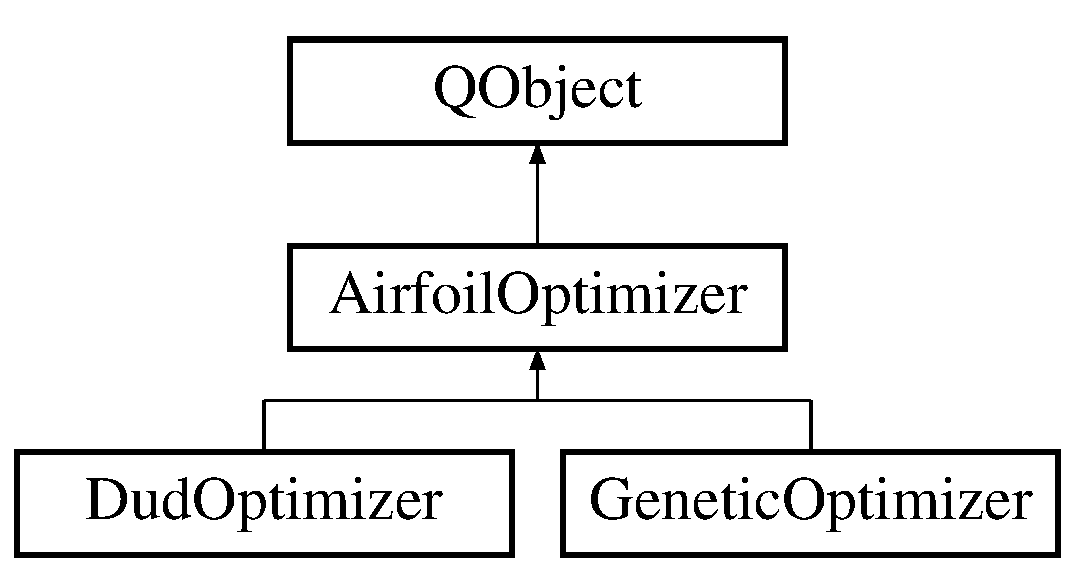
\includegraphics[height=3.000000cm]{class_airfoil_optimizer}
\end{center}
\end{figure}
\subsection*{Signals}
\begin{DoxyCompactItemize}
\item 
\mbox{\Hypertarget{class_airfoil_optimizer_ab9c9cba16c69c178be6344c7d57794aa}\label{class_airfoil_optimizer_ab9c9cba16c69c178be6344c7d57794aa}} 
void {\bfseries optimization\+Finished} ()
\end{DoxyCompactItemize}
\subsection*{Public Member Functions}
\begin{DoxyCompactItemize}
\item 
\mbox{\Hypertarget{class_airfoil_optimizer_a6547cf20afd5820b7ce961e5777d02a6}\label{class_airfoil_optimizer_a6547cf20afd5820b7ce961e5777d02a6}} 
virtual void {\bfseries initialize} (\hyperlink{class_geometry}{Geometry} \&geom)=0
\item 
\mbox{\Hypertarget{class_airfoil_optimizer_abe159aa3cef40f5b25ecca8fab1353d1}\label{class_airfoil_optimizer_abe159aa3cef40f5b25ecca8fab1353d1}} 
virtual void {\bfseries optimize\+Step} ()=0
\item 
\mbox{\Hypertarget{class_airfoil_optimizer_af97435c1a0351b2ed9597a5c522e7c7f}\label{class_airfoil_optimizer_af97435c1a0351b2ed9597a5c522e7c7f}} 
virtual \hyperlink{class_geometry}{Geometry} const {\bfseries get\+Top\+Geometry} ()=0
\item 
\mbox{\Hypertarget{class_airfoil_optimizer_a5180dad58c1256ca4909e497f1c2b516}\label{class_airfoil_optimizer_a5180dad58c1256ca4909e497f1c2b516}} 
virtual double const {\bfseries get\+Progress} ()=0
\end{DoxyCompactItemize}


\subsection{Detailed Description}
Abstract Airfoil optimizer object for managing Optimization and communication with model. 

Allows for multiple optimizer implementations 

The documentation for this class was generated from the following file\+:\begin{DoxyCompactItemize}
\item 
optimizer/\hyperlink{airfoil__optimizer_8h}{airfoil\+\_\+optimizer.\+h}\end{DoxyCompactItemize}

\hypertarget{struct_config_1_1_application_params}{}\section{Config\+:\+:Application\+Params Struct Reference}
\label{struct_config_1_1_application_params}\index{Config\+::\+Application\+Params@{Config\+::\+Application\+Params}}


The documentation for this struct was generated from the following file\+:\begin{DoxyCompactItemize}
\item 
utility/\hyperlink{config_8h}{config.\+h}\end{DoxyCompactItemize}

\hypertarget{struct_aviation_profile_parameters}{}\section{Aviation\+Profile\+Parameters Struct Reference}
\label{struct_aviation_profile_parameters}\index{Aviation\+Profile\+Parameters@{Aviation\+Profile\+Parameters}}


Struct consists airfoil basic parameters.  




{\ttfamily \#include $<$profile\+\_\+parameters.\+h$>$}

\subsection*{Public Attributes}
\begin{DoxyCompactItemize}
\item 
\mbox{\Hypertarget{struct_aviation_profile_parameters_a193e4e8fe42f26ed6352fdf7cb438f7c}\label{struct_aviation_profile_parameters_a193e4e8fe42f26ed6352fdf7cb438f7c}} 
double {\bfseries alfa} = -\/1
\item 
\mbox{\Hypertarget{struct_aviation_profile_parameters_a5aa0cd7099bde735f7fe27020ec9c508}\label{struct_aviation_profile_parameters_a5aa0cd7099bde735f7fe27020ec9c508}} 
double {\bfseries cl\+Max} = -\/1
\item 
\mbox{\Hypertarget{struct_aviation_profile_parameters_a8fa1990f36d8bc9be69a5e993bbf1516}\label{struct_aviation_profile_parameters_a8fa1990f36d8bc9be69a5e993bbf1516}} 
double {\bfseries cd\+Min} = -\/1
\end{DoxyCompactItemize}


\subsection{Detailed Description}
Struct consists airfoil basic parameters. 

The documentation for this struct was generated from the following file\+:\begin{DoxyCompactItemize}
\item 
model/\hyperlink{profile__parameters_8h}{profile\+\_\+parameters.\+h}\end{DoxyCompactItemize}

\hypertarget{struct_binary_airfoil_coefficients}{}\section{Binary\+Airfoil\+Coefficients Struct Reference}
\label{struct_binary_airfoil_coefficients}\index{Binary\+Airfoil\+Coefficients@{Binary\+Airfoil\+Coefficients}}


{\ttfamily \#include $<$geometry\+\_\+structures.\+h$>$}

\subsection*{Public Member Functions}
\begin{DoxyCompactItemize}
\item 
\mbox{\Hypertarget{struct_binary_airfoil_coefficients_a1a7fcb4d52f90f94d0fca535897a5428}\label{struct_binary_airfoil_coefficients_a1a7fcb4d52f90f94d0fca535897a5428}} 
\hyperlink{struct_binary_airfoil_coefficients}{Binary\+Airfoil\+Coefficients} \& {\bfseries operator=} (const \hyperlink{struct_binary_airfoil_coefficients}{Binary\+Airfoil\+Coefficients} \&data)
\end{DoxyCompactItemize}
\subsection*{Public Attributes}
\begin{DoxyCompactItemize}
\item 
byte \hyperlink{struct_binary_airfoil_coefficients_adc5da813d292a991f0e038348ff26ae1}{p\+\_\+u}
\item 
byte \hyperlink{struct_binary_airfoil_coefficients_a9474385e776695d50b75914ff62bd37a}{p\+\_\+l}
\item 
byte \hyperlink{struct_binary_airfoil_coefficients_a2fd01b5ce7c9bef55ba5e30bd19c062a}{a\+\_\+u}
\item 
byte \hyperlink{struct_binary_airfoil_coefficients_a49511b7e8398b06d8d880c7576ab5311}{a\+\_\+l}
\item 
byte \hyperlink{struct_binary_airfoil_coefficients_adadc9038b8731917b4dbcabd776b6627}{b\+\_\+u}
\item 
byte \hyperlink{struct_binary_airfoil_coefficients_a3d553603f76f7b5ddc6febc3a70db3f3}{b\+\_\+l}
\item 
byte \hyperlink{struct_binary_airfoil_coefficients_a6ed8c98c3817a396756b2a16a0d4791b}{q\+\_\+u}
\item 
byte \hyperlink{struct_binary_airfoil_coefficients_af015cf807e794441f030791862b22adb}{q\+\_\+l}
\item 
byte \hyperlink{struct_binary_airfoil_coefficients_a9de0fabddae28b4d649a256c19137eb4}{c\+\_\+u}
\item 
byte \hyperlink{struct_binary_airfoil_coefficients_a0c5c811277770502ff707312b5289601}{c\+\_\+l}
\item 
byte \hyperlink{struct_binary_airfoil_coefficients_a9640283446988bbdb012e94aaf2a41a3}{d\+\_\+u}
\item 
byte \hyperlink{struct_binary_airfoil_coefficients_a8b911d241a95f63e79813747ba2c25e6}{d\+\_\+l}
\end{DoxyCompactItemize}


\subsection{Detailed Description}
Param become larger\+: Overall shape becomeshigher Param become smaller\+: Overall shape becomes lower 

\subsection{Member Data Documentation}
\mbox{\Hypertarget{struct_binary_airfoil_coefficients_a49511b7e8398b06d8d880c7576ab5311}\label{struct_binary_airfoil_coefficients_a49511b7e8398b06d8d880c7576ab5311}} 
\index{Binary\+Airfoil\+Coefficients@{Binary\+Airfoil\+Coefficients}!a\+\_\+l@{a\+\_\+l}}
\index{a\+\_\+l@{a\+\_\+l}!Binary\+Airfoil\+Coefficients@{Binary\+Airfoil\+Coefficients}}
\subsubsection{\texorpdfstring{a\+\_\+l}{a\_l}}
{\footnotesize\ttfamily Binary\+Airfoil\+Coefficients\+::a\+\_\+l}

Param become larger\+: Back part becomes lower significantly; Forepart part becomes lower slightly Param become smaller\+: Back part becomes higher significantly; Forepart becomes higher slightly \mbox{\Hypertarget{struct_binary_airfoil_coefficients_a2fd01b5ce7c9bef55ba5e30bd19c062a}\label{struct_binary_airfoil_coefficients_a2fd01b5ce7c9bef55ba5e30bd19c062a}} 
\index{Binary\+Airfoil\+Coefficients@{Binary\+Airfoil\+Coefficients}!a\+\_\+u@{a\+\_\+u}}
\index{a\+\_\+u@{a\+\_\+u}!Binary\+Airfoil\+Coefficients@{Binary\+Airfoil\+Coefficients}}
\subsubsection{\texorpdfstring{a\+\_\+u}{a\_u}}
{\footnotesize\ttfamily Binary\+Airfoil\+Coefficients\+::a\+\_\+u}

Param become larger\+: Forepart becomes lower significantly; Back part becomes lower slightly Param become smaller\+: Forepart becomes higher significantly; Back part becomes higher slightly \mbox{\Hypertarget{struct_binary_airfoil_coefficients_a3d553603f76f7b5ddc6febc3a70db3f3}\label{struct_binary_airfoil_coefficients_a3d553603f76f7b5ddc6febc3a70db3f3}} 
\index{Binary\+Airfoil\+Coefficients@{Binary\+Airfoil\+Coefficients}!b\+\_\+l@{b\+\_\+l}}
\index{b\+\_\+l@{b\+\_\+l}!Binary\+Airfoil\+Coefficients@{Binary\+Airfoil\+Coefficients}}
\subsubsection{\texorpdfstring{b\+\_\+l}{b\_l}}
{\footnotesize\ttfamily Binary\+Airfoil\+Coefficients\+::b\+\_\+l}

Param become larger\+: Overall shape becomes thicker Param become smaller\+: Overall shape becomes thinner \mbox{\Hypertarget{struct_binary_airfoil_coefficients_adadc9038b8731917b4dbcabd776b6627}\label{struct_binary_airfoil_coefficients_adadc9038b8731917b4dbcabd776b6627}} 
\index{Binary\+Airfoil\+Coefficients@{Binary\+Airfoil\+Coefficients}!b\+\_\+u@{b\+\_\+u}}
\index{b\+\_\+u@{b\+\_\+u}!Binary\+Airfoil\+Coefficients@{Binary\+Airfoil\+Coefficients}}
\subsubsection{\texorpdfstring{b\+\_\+u}{b\_u}}
{\footnotesize\ttfamily Binary\+Airfoil\+Coefficients\+::b\+\_\+u}

Param become larger\+: Back part becomes lower significantly; Forepart part becomes lower slightly Param become smaller\+: Back part becomes higher significantly; Forepart becomes higher slightly \mbox{\Hypertarget{struct_binary_airfoil_coefficients_a0c5c811277770502ff707312b5289601}\label{struct_binary_airfoil_coefficients_a0c5c811277770502ff707312b5289601}} 
\index{Binary\+Airfoil\+Coefficients@{Binary\+Airfoil\+Coefficients}!c\+\_\+l@{c\+\_\+l}}
\index{c\+\_\+l@{c\+\_\+l}!Binary\+Airfoil\+Coefficients@{Binary\+Airfoil\+Coefficients}}
\subsubsection{\texorpdfstring{c\+\_\+l}{c\_l}}
{\footnotesize\ttfamily Binary\+Airfoil\+Coefficients\+::c\+\_\+l}

Param become larger\+: Back part becomes thinner significantly; Forepart becomes thinner slightly Param become smaller\+: Back part becomes thicker significantly; Forepart becomes thicker slightly \mbox{\Hypertarget{struct_binary_airfoil_coefficients_a9de0fabddae28b4d649a256c19137eb4}\label{struct_binary_airfoil_coefficients_a9de0fabddae28b4d649a256c19137eb4}} 
\index{Binary\+Airfoil\+Coefficients@{Binary\+Airfoil\+Coefficients}!c\+\_\+u@{c\+\_\+u}}
\index{c\+\_\+u@{c\+\_\+u}!Binary\+Airfoil\+Coefficients@{Binary\+Airfoil\+Coefficients}}
\subsubsection{\texorpdfstring{c\+\_\+u}{c\_u}}
{\footnotesize\ttfamily Binary\+Airfoil\+Coefficients\+::c\+\_\+u}

Param become larger\+: Forepart becomes thinner significantly; Back part becomes thinner slightly Param become smaller\+: Forepart becomes thicker significantly; Back part becomes thicker slightly \mbox{\Hypertarget{struct_binary_airfoil_coefficients_a8b911d241a95f63e79813747ba2c25e6}\label{struct_binary_airfoil_coefficients_a8b911d241a95f63e79813747ba2c25e6}} 
\index{Binary\+Airfoil\+Coefficients@{Binary\+Airfoil\+Coefficients}!d\+\_\+l@{d\+\_\+l}}
\index{d\+\_\+l@{d\+\_\+l}!Binary\+Airfoil\+Coefficients@{Binary\+Airfoil\+Coefficients}}
\subsubsection{\texorpdfstring{d\+\_\+l}{d\_l}}
{\footnotesize\ttfamily Binary\+Airfoil\+Coefficients\+::d\+\_\+l}

\begin{DoxyAuthor}{Author}
Jakub Polaczek \& Hubert Buczyński 
\end{DoxyAuthor}
\begin{DoxyDate}{Date}
05/06/2017 
\end{DoxyDate}
\mbox{\Hypertarget{struct_binary_airfoil_coefficients_a9640283446988bbdb012e94aaf2a41a3}\label{struct_binary_airfoil_coefficients_a9640283446988bbdb012e94aaf2a41a3}} 
\index{Binary\+Airfoil\+Coefficients@{Binary\+Airfoil\+Coefficients}!d\+\_\+u@{d\+\_\+u}}
\index{d\+\_\+u@{d\+\_\+u}!Binary\+Airfoil\+Coefficients@{Binary\+Airfoil\+Coefficients}}
\subsubsection{\texorpdfstring{d\+\_\+u}{d\_u}}
{\footnotesize\ttfamily Binary\+Airfoil\+Coefficients\+::d\+\_\+u}

Param become larger\+: Back part becomes thinner significantly; Forepart becomes thinner slightly Param become smaller\+: Back part becomes thicker significantly; Forepart becomes thicker slightly \mbox{\Hypertarget{struct_binary_airfoil_coefficients_a9474385e776695d50b75914ff62bd37a}\label{struct_binary_airfoil_coefficients_a9474385e776695d50b75914ff62bd37a}} 
\index{Binary\+Airfoil\+Coefficients@{Binary\+Airfoil\+Coefficients}!p\+\_\+l@{p\+\_\+l}}
\index{p\+\_\+l@{p\+\_\+l}!Binary\+Airfoil\+Coefficients@{Binary\+Airfoil\+Coefficients}}
\subsubsection{\texorpdfstring{p\+\_\+l}{p\_l}}
{\footnotesize\ttfamily Binary\+Airfoil\+Coefficients\+::p\+\_\+l}

Param become larger\+: Forepart becomes lower significantly; Back part becomes lower slightly Param become smaller\+: Forepart becomes higher significantly; Back part becomes higher slightly \mbox{\Hypertarget{struct_binary_airfoil_coefficients_adc5da813d292a991f0e038348ff26ae1}\label{struct_binary_airfoil_coefficients_adc5da813d292a991f0e038348ff26ae1}} 
\index{Binary\+Airfoil\+Coefficients@{Binary\+Airfoil\+Coefficients}!p\+\_\+u@{p\+\_\+u}}
\index{p\+\_\+u@{p\+\_\+u}!Binary\+Airfoil\+Coefficients@{Binary\+Airfoil\+Coefficients}}
\subsubsection{\texorpdfstring{p\+\_\+u}{p\_u}}
{\footnotesize\ttfamily Binary\+Airfoil\+Coefficients\+::p\+\_\+u}

Param become larger\+: Overall shape becomeshigher Param become smaller\+: Overall shape becomes lower \mbox{\Hypertarget{struct_binary_airfoil_coefficients_af015cf807e794441f030791862b22adb}\label{struct_binary_airfoil_coefficients_af015cf807e794441f030791862b22adb}} 
\index{Binary\+Airfoil\+Coefficients@{Binary\+Airfoil\+Coefficients}!q\+\_\+l@{q\+\_\+l}}
\index{q\+\_\+l@{q\+\_\+l}!Binary\+Airfoil\+Coefficients@{Binary\+Airfoil\+Coefficients}}
\subsubsection{\texorpdfstring{q\+\_\+l}{q\_l}}
{\footnotesize\ttfamily Binary\+Airfoil\+Coefficients\+::q\+\_\+l}

Param become larger\+: Forepart becomes thinner significantly; Back part becomes thinner slightly Param become smaller\+: Forepart becomes thicker significantly; Back part becomes thicker slightly \mbox{\Hypertarget{struct_binary_airfoil_coefficients_a6ed8c98c3817a396756b2a16a0d4791b}\label{struct_binary_airfoil_coefficients_a6ed8c98c3817a396756b2a16a0d4791b}} 
\index{Binary\+Airfoil\+Coefficients@{Binary\+Airfoil\+Coefficients}!q\+\_\+u@{q\+\_\+u}}
\index{q\+\_\+u@{q\+\_\+u}!Binary\+Airfoil\+Coefficients@{Binary\+Airfoil\+Coefficients}}
\subsubsection{\texorpdfstring{q\+\_\+u}{q\_u}}
{\footnotesize\ttfamily Binary\+Airfoil\+Coefficients\+::q\+\_\+u}

Param become larger\+: Overall shape becomes thicker Param become smaller\+: Overall shape becomes thinner 

The documentation for this struct was generated from the following file\+:\begin{DoxyCompactItemize}
\item 
optimizer/\hyperlink{geometry__structures_8h}{geometry\+\_\+structures.\+h}\end{DoxyCompactItemize}

\hypertarget{struct_component}{}\section{Component Struct Reference}
\label{struct_component}\index{Component@{Component}}
\subsection*{Public Attributes}
\begin{DoxyCompactItemize}
\item 
\hypertarget{struct_component_aa0cd0fd532b68947f1d6f6f50ca76700}{}\label{struct_component_aa0cd0fd532b68947f1d6f6f50ca76700} 
Q\+Object $\ast$ {\bfseries object}
\item 
\hypertarget{struct_component_a46343549452bda5ee9752f7a9bc15efb}{}\label{struct_component_a46343549452bda5ee9752f7a9bc15efb} 
std\+::string {\bfseries name}
\end{DoxyCompactItemize}


The documentation for this struct was generated from the following file\+:\begin{DoxyCompactItemize}
\item 
gui/\hyperlink{gui__objects_8h}{gui\+\_\+objects.\+h}\end{DoxyCompactItemize}

\hypertarget{class_config}{}\section{Config Class Reference}
\label{class_config}\index{Config@{Config}}


Class containing application parameters.  




{\ttfamily \#include $<$config.\+h$>$}

\subsection*{Classes}
\begin{DoxyCompactItemize}
\item 
struct \hyperlink{struct_config_1_1_application_params}{Application\+Params}
\item 
struct \hyperlink{struct_config_1_1_optimizer_params}{Optimizer\+Params}
\item 
struct \hyperlink{struct_config_1_1_simulation_params}{Simulation\+Params}
\end{DoxyCompactItemize}


\subsection{Detailed Description}
Class containing application parameters. 

This class consists basic structures use in the whole application. 

The documentation for this class was generated from the following file\+:\begin{DoxyCompactItemize}
\item 
utility/\hyperlink{config_8h}{config.\+h}\end{DoxyCompactItemize}

\hypertarget{class_configuration_reader}{}\section{Configuration\+Reader Class Reference}
\label{class_configuration_reader}\index{Configuration\+Reader@{Configuration\+Reader}}


Class containing methods to generate and load parameters from xml file.  




{\ttfamily \#include $<$configuration\+\_\+reader.\+h$>$}

\subsection*{Public Member Functions}
\begin{DoxyCompactItemize}
\item 
\hypertarget{class_configuration_reader_a48396fe5ae72fe84728917c4d3c1d873}{}\label{class_configuration_reader_a48396fe5ae72fe84728917c4d3c1d873} 
bool {\bfseries initialize} ()
\item 
\hypertarget{class_configuration_reader_a8a9b59775e830c242e3a11ac7b1e60c4}{}\label{class_configuration_reader_a8a9b59775e830c242e3a11ac7b1e60c4} 
\hyperlink{struct_config_1_1_application_params}{Config\+::\+Application\+Params} {\bfseries get\+Application\+Parameters} ()
\item 
\hypertarget{class_configuration_reader_a26229de2dab15c900a09c8b3a2587a90}{}\label{class_configuration_reader_a26229de2dab15c900a09c8b3a2587a90} 
\hyperlink{struct_config_1_1_optimizer_params}{Config\+::\+Optimizer\+Params} {\bfseries get\+Optimizer\+Parameters} ()
\item 
\hypertarget{class_configuration_reader_a9a8d35884446e5d4c5beb769445f3b49}{}\label{class_configuration_reader_a9a8d35884446e5d4c5beb769445f3b49} 
\hyperlink{struct_config_1_1_simulation_params}{Config\+::\+Simulation\+Params} {\bfseries get\+Simulator\+Parameters} ()
\end{DoxyCompactItemize}
\subsection*{Static Public Member Functions}
\begin{DoxyCompactItemize}
\item 
\hypertarget{class_configuration_reader_a48d64d4b30e6b952848f95295cc6aae8}{}\label{class_configuration_reader_a48d64d4b30e6b952848f95295cc6aae8} 
static std\+::string {\bfseries get\+Project\+Path} ()
\item 
\hypertarget{class_configuration_reader_a8dd351a562599f9017911c9564b06716}{}\label{class_configuration_reader_a8dd351a562599f9017911c9564b06716} 
static std\+::string {\bfseries get\+Parameter\+File\+Path} ()
\item 
\hypertarget{class_configuration_reader_a2744da82a66457674996be080d2f37d8}{}\label{class_configuration_reader_a2744da82a66457674996be080d2f37d8} 
static std\+::string {\bfseries get\+Separator} ()
\end{DoxyCompactItemize}


\subsection{Detailed Description}
Class containing methods to generate and load parameters from xml file. 

This class uses Tiny\+Xml library to write and read data to xml files. 

The documentation for this class was generated from the following files\+:\begin{DoxyCompactItemize}
\item 
utility/\hyperlink{configuration__reader_8h}{configuration\+\_\+reader.\+h}\item 
utility/configuration\+\_\+reader.\+cpp\end{DoxyCompactItemize}

\hypertarget{class_dud_optimizer}{}\section{Dud\+Optimizer Class Reference}
\label{class_dud_optimizer}\index{Dud\+Optimizer@{Dud\+Optimizer}}


Dud Airfoil optimizer object for testing interfaces.  




{\ttfamily \#include $<$airfoil\+\_\+optimizer.\+h$>$}

Inheritance diagram for Dud\+Optimizer\+:\begin{figure}[H]
\begin{center}
\leavevmode
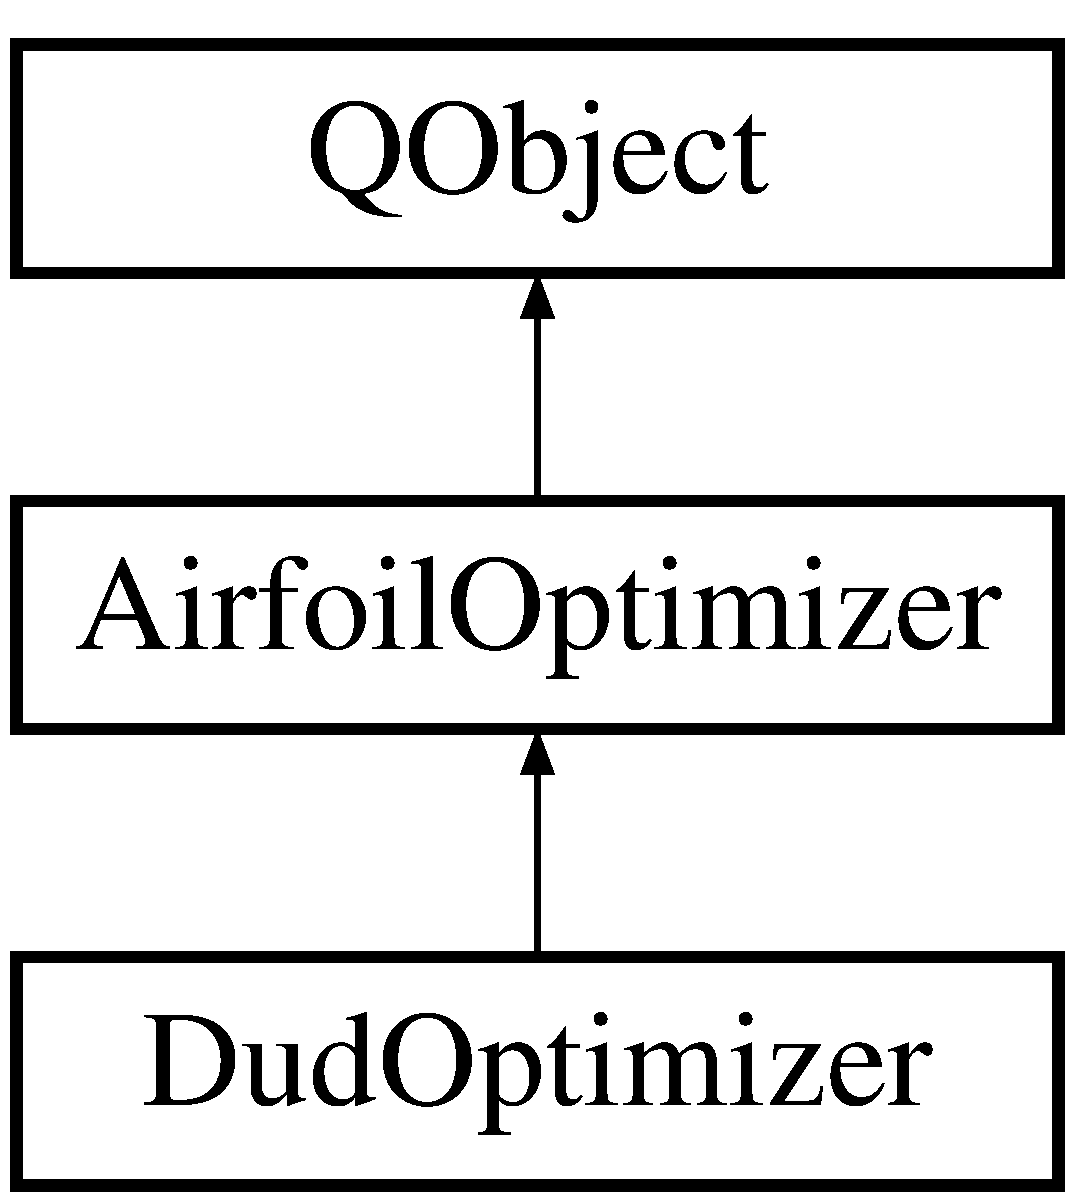
\includegraphics[height=3.000000cm]{class_dud_optimizer}
\end{center}
\end{figure}
\subsection*{Public Member Functions}
\begin{DoxyCompactItemize}
\item 
\mbox{\Hypertarget{class_dud_optimizer_af26b9a7008edc72eab4904e4412ec807}\label{class_dud_optimizer_af26b9a7008edc72eab4904e4412ec807}} 
{\bfseries Dud\+Optimizer} (\hyperlink{class_geometry}{Geometry} \&geom)
\item 
\mbox{\Hypertarget{class_dud_optimizer_a1cab6b6d9290cd8b573946eae396ac4a}\label{class_dud_optimizer_a1cab6b6d9290cd8b573946eae396ac4a}} 
virtual void {\bfseries initialize} (\hyperlink{class_geometry}{Geometry} \&geom) override
\item 
\mbox{\Hypertarget{class_dud_optimizer_a6bb45a864903a58c7b030f94f388e094}\label{class_dud_optimizer_a6bb45a864903a58c7b030f94f388e094}} 
virtual void {\bfseries optimize\+Step} () override
\item 
\mbox{\Hypertarget{class_dud_optimizer_af20d6c98319f93ea3d3ee82736900eb5}\label{class_dud_optimizer_af20d6c98319f93ea3d3ee82736900eb5}} 
virtual \hyperlink{class_geometry}{Geometry} const {\bfseries get\+Top\+Geometry} () override
\item 
\mbox{\Hypertarget{class_dud_optimizer_ac5cb8e4b437fb0bd9584541e43939809}\label{class_dud_optimizer_ac5cb8e4b437fb0bd9584541e43939809}} 
virtual double const {\bfseries get\+Progress} () override
\end{DoxyCompactItemize}
\subsection*{Additional Inherited Members}


\subsection{Detailed Description}
Dud Airfoil optimizer object for testing interfaces. 

Allows for different test scenarios 

The documentation for this class was generated from the following file\+:\begin{DoxyCompactItemize}
\item 
optimizer/\hyperlink{airfoil__optimizer_8h}{airfoil\+\_\+optimizer.\+h}\end{DoxyCompactItemize}

\hypertarget{class_dud_scrambler}{}\section{Dud\+Scrambler Class Reference}
\label{class_dud_scrambler}\index{Dud\+Scrambler@{Dud\+Scrambler}}


Test class for Genetic\+Scrambler objects.  




{\ttfamily \#include $<$genome\+\_\+scrambler.\+h$>$}

Inheritance diagram for Dud\+Scrambler\+:\begin{figure}[H]
\begin{center}
\leavevmode
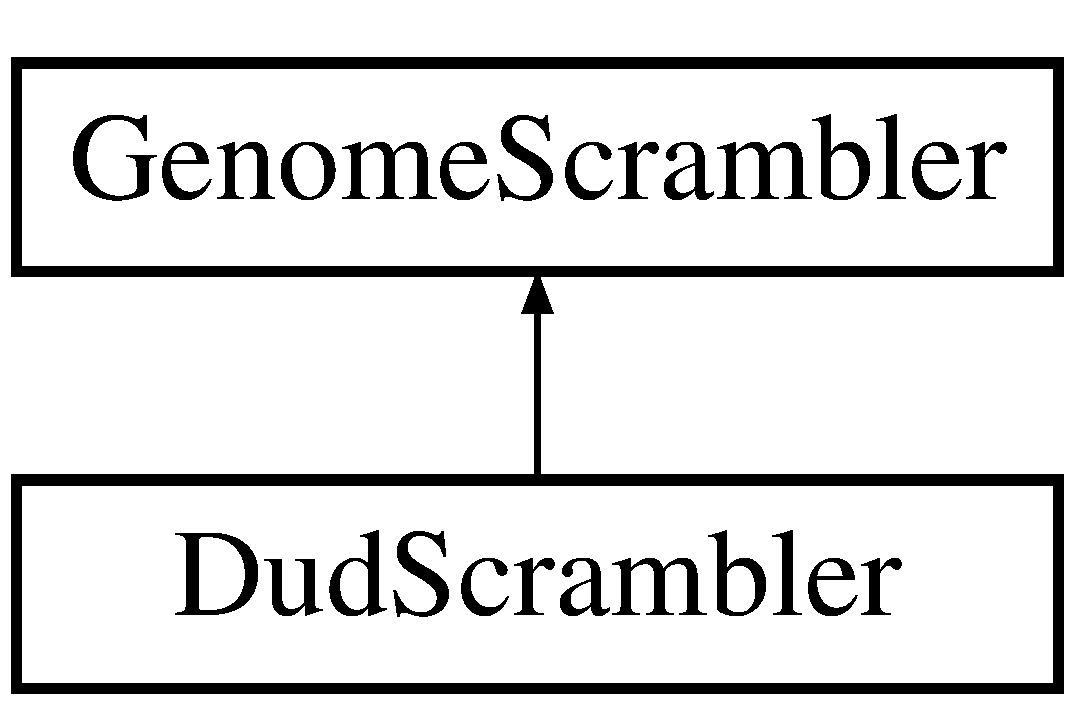
\includegraphics[height=2.000000cm]{class_dud_scrambler}
\end{center}
\end{figure}
\subsection*{Public Member Functions}
\begin{DoxyCompactItemize}
\item 
\mbox{\Hypertarget{class_dud_scrambler_a9fd7e425f2ca563c7c72ae0e1926e238}\label{class_dud_scrambler_a9fd7e425f2ca563c7c72ae0e1926e238}} 
virtual \hyperlink{class_genome}{Genome} $\ast$ {\bfseries mutate} (\hyperlink{class_genome}{Genome} $\ast$genome) override
\item 
\mbox{\Hypertarget{class_dud_scrambler_a6d3491d703d0b3a60316349d97d1587a}\label{class_dud_scrambler_a6d3491d703d0b3a60316349d97d1587a}} 
virtual \hyperlink{class_genome}{Genome} $\ast$ {\bfseries crossover} (\hyperlink{class_genome}{Genome} $\ast$g1, \hyperlink{class_genome}{Genome} $\ast$g2) override
\end{DoxyCompactItemize}


\subsection{Detailed Description}
Test class for Genetic\+Scrambler objects. 

\hyperlink{class_dud_scrambler}{Dud\+Scrambler} object is a test object providing constant, not random implementation for scrambling 

The documentation for this class was generated from the following files\+:\begin{DoxyCompactItemize}
\item 
optimizer/genetic/\hyperlink{genome__scrambler_8h}{genome\+\_\+scrambler.\+h}\item 
optimizer/genetic/genome\+\_\+scrambler.\+cpp\end{DoxyCompactItemize}

\hypertarget{struct_exception_handler}{}\section{Exception\+Handler Struct Reference}
\label{struct_exception_handler}\index{Exception\+Handler@{Exception\+Handler}}


Exception Handler.  




{\ttfamily \#include $<$utility.\+h$>$}

Inheritance diagram for Exception\+Handler\+:\begin{figure}[H]
\begin{center}
\leavevmode
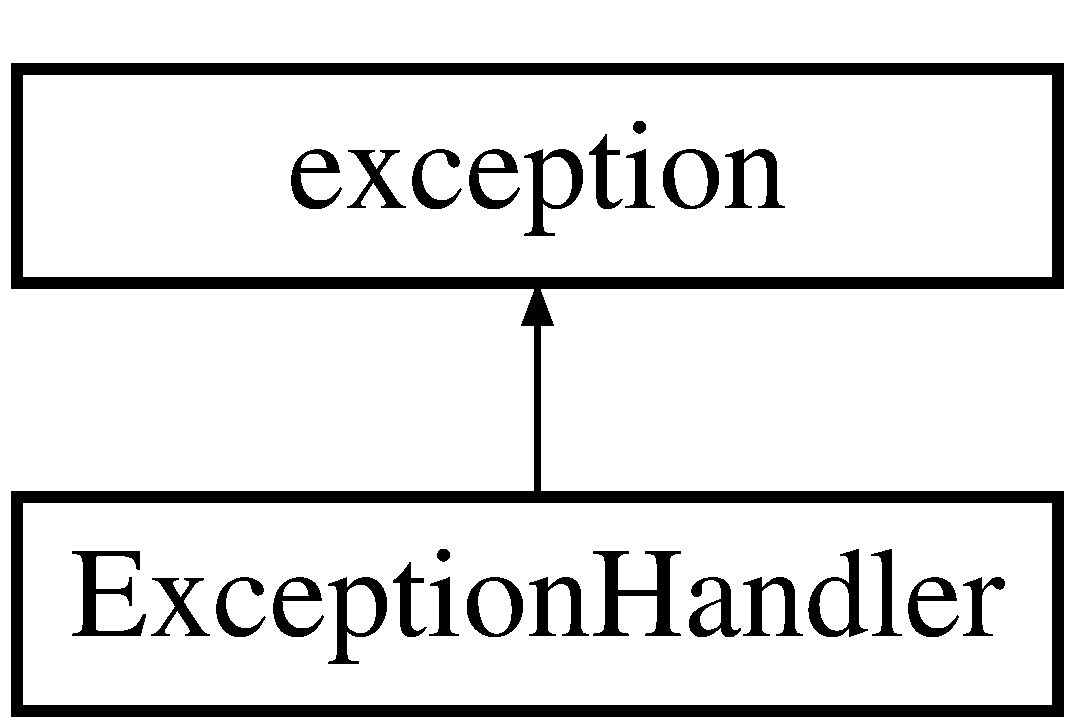
\includegraphics[height=2.000000cm]{struct_exception_handler}
\end{center}
\end{figure}
\subsection*{Public Member Functions}
\begin{DoxyCompactItemize}
\item 
\hypertarget{struct_exception_handler_ae134c5213991a7b0983cdf8891a5f9e8}{}\label{struct_exception_handler_ae134c5213991a7b0983cdf8891a5f9e8} 
{\bfseries Exception\+Handler} (const std\+::string \&ex)
\end{DoxyCompactItemize}
\subsection*{Public Attributes}
\begin{DoxyCompactItemize}
\item 
\hypertarget{struct_exception_handler_ae18ca9e51660276419ca7e35d0b0db1c}{}\label{struct_exception_handler_ae18ca9e51660276419ca7e35d0b0db1c} 
std\+::string {\bfseries e}
\end{DoxyCompactItemize}


\subsection{Detailed Description}
Exception Handler. 

The documentation for this struct was generated from the following files\+:\begin{DoxyCompactItemize}
\item 
utility/\hyperlink{utility_8h}{utility.\+h}\item 
utility/utility.\+cpp\end{DoxyCompactItemize}

\hypertarget{struct_config_1_1_optimizer_params_1_1_fitness}{}\section{Config\+:\+:Optimizer\+Params\+:\+:Fitness Struct Reference}
\label{struct_config_1_1_optimizer_params_1_1_fitness}\index{Config\+::\+Optimizer\+Params\+::\+Fitness@{Config\+::\+Optimizer\+Params\+::\+Fitness}}
\subsection*{Public Attributes}
\begin{DoxyCompactItemize}
\item 
\mbox{\Hypertarget{struct_config_1_1_optimizer_params_1_1_fitness_a200cf3c64e202394decaec34d89bd280}\label{struct_config_1_1_optimizer_params_1_1_fitness_a200cf3c64e202394decaec34d89bd280}} 
bool {\bfseries optimize\+Stall} = false
\item 
\mbox{\Hypertarget{struct_config_1_1_optimizer_params_1_1_fitness_afbb10a58397284eeabc89a951ee3d467}\label{struct_config_1_1_optimizer_params_1_1_fitness_afbb10a58397284eeabc89a951ee3d467}} 
bool {\bfseries optimize\+Cl} = true
\item 
\mbox{\Hypertarget{struct_config_1_1_optimizer_params_1_1_fitness_a8175a4e1d6d67dee007591263c78053b}\label{struct_config_1_1_optimizer_params_1_1_fitness_a8175a4e1d6d67dee007591263c78053b}} 
bool {\bfseries optimize\+Cd} = true
\item 
\mbox{\Hypertarget{struct_config_1_1_optimizer_params_1_1_fitness_a9cade69b8a94f7400d0136d85f84832e}\label{struct_config_1_1_optimizer_params_1_1_fitness_a9cade69b8a94f7400d0136d85f84832e}} 
bool {\bfseries optimize\+Glide} = false
\item 
\mbox{\Hypertarget{struct_config_1_1_optimizer_params_1_1_fitness_ac5978cb103bc4761ddb8411edf237ba7}\label{struct_config_1_1_optimizer_params_1_1_fitness_ac5978cb103bc4761ddb8411edf237ba7}} 
bool {\bfseries optimize\+Moment} = false
\item 
\mbox{\Hypertarget{struct_config_1_1_optimizer_params_1_1_fitness_a01359bf3a0aff54006267de6e52301b8}\label{struct_config_1_1_optimizer_params_1_1_fitness_a01359bf3a0aff54006267de6e52301b8}} 
double {\bfseries target\+Cl} = 1.\+3
\item 
\mbox{\Hypertarget{struct_config_1_1_optimizer_params_1_1_fitness_ab41096bb4d5ea5bf319e7d9db250d081}\label{struct_config_1_1_optimizer_params_1_1_fitness_ab41096bb4d5ea5bf319e7d9db250d081}} 
double {\bfseries target\+Cd} = 0.\+01
\item 
\mbox{\Hypertarget{struct_config_1_1_optimizer_params_1_1_fitness_a2c546c543c4b37f14ccb2212f5ccb106}\label{struct_config_1_1_optimizer_params_1_1_fitness_a2c546c543c4b37f14ccb2212f5ccb106}} 
double {\bfseries target\+Glide} = 120.\+0
\item 
\mbox{\Hypertarget{struct_config_1_1_optimizer_params_1_1_fitness_af9ae034f5b96580c4d6d56885b120472}\label{struct_config_1_1_optimizer_params_1_1_fitness_af9ae034f5b96580c4d6d56885b120472}} 
double {\bfseries target\+Stall\+Alfa} = 12.\+0
\item 
\mbox{\Hypertarget{struct_config_1_1_optimizer_params_1_1_fitness_aca32b706fb91fd4283e50d2b0bd5c077}\label{struct_config_1_1_optimizer_params_1_1_fitness_aca32b706fb91fd4283e50d2b0bd5c077}} 
double {\bfseries target\+Moment} = 0.\+115
\item 
\mbox{\Hypertarget{struct_config_1_1_optimizer_params_1_1_fitness_a131f6e3214620d90b03e16be286aad56}\label{struct_config_1_1_optimizer_params_1_1_fitness_a131f6e3214620d90b03e16be286aad56}} 
double {\bfseries weight\+Cl} =1000.\+0
\item 
\mbox{\Hypertarget{struct_config_1_1_optimizer_params_1_1_fitness_ad515ada424e92bd3f963fdcd4c63ba03}\label{struct_config_1_1_optimizer_params_1_1_fitness_ad515ada424e92bd3f963fdcd4c63ba03}} 
double {\bfseries weight\+Cd} = 500.\+0
\item 
\mbox{\Hypertarget{struct_config_1_1_optimizer_params_1_1_fitness_aef5f76da9704838a2caf0c4a9ae712b1}\label{struct_config_1_1_optimizer_params_1_1_fitness_aef5f76da9704838a2caf0c4a9ae712b1}} 
double {\bfseries weight\+Glide} = 1000.\+0
\item 
\mbox{\Hypertarget{struct_config_1_1_optimizer_params_1_1_fitness_ad9ffb0836c80c0ddcb483c661fc6f42a}\label{struct_config_1_1_optimizer_params_1_1_fitness_ad9ffb0836c80c0ddcb483c661fc6f42a}} 
double {\bfseries weight\+Stall} = 500.\+0
\item 
\mbox{\Hypertarget{struct_config_1_1_optimizer_params_1_1_fitness_ae348e127a5fe28e28b8cbe7cb0aea68f}\label{struct_config_1_1_optimizer_params_1_1_fitness_ae348e127a5fe28e28b8cbe7cb0aea68f}} 
double {\bfseries weight\+Moment} = 100.\+0
\end{DoxyCompactItemize}


The documentation for this struct was generated from the following file\+:\begin{DoxyCompactItemize}
\item 
utility/\hyperlink{config_8h}{config.\+h}\end{DoxyCompactItemize}

\hypertarget{class_fitness_model}{}\section{Fitness\+Model Class Reference}
\label{class_fitness_model}\index{Fitness\+Model@{Fitness\+Model}}


Class maintain fitness function for genetic algorithm.  




{\ttfamily \#include $<$fitness.\+h$>$}

\subsection*{Public Member Functions}
\begin{DoxyCompactItemize}
\item 
\hypertarget{class_fitness_model_a3965cdc6d87b01d3ecef12c9f9653995}{}\label{class_fitness_model_a3965cdc6d87b01d3ecef12c9f9653995} 
{\bfseries Fitness\+Model} (\hyperlink{struct_config_1_1_optimizer_params_1_1_fitness}{Config\+::\+Optimizer\+Params\+::\+Fitness} params)
\item 
\hypertarget{class_fitness_model_a25a721689cc99d5691a6e8ad8d36bbf6}{}\label{class_fitness_model_a25a721689cc99d5691a6e8ad8d36bbf6} 
double {\bfseries Calculate} (const \hyperlink{class_sim_results}{Sim\+Results} \&results)
\end{DoxyCompactItemize}


\subsection{Detailed Description}
Class maintain fitness function for genetic algorithm. 

Calculate fitness for each genome in population 

The documentation for this class was generated from the following files\+:\begin{DoxyCompactItemize}
\item 
optimizer/genetic/\hyperlink{fitness_8h}{fitness.\+h}\item 
optimizer/genetic/fitness.\+cpp\end{DoxyCompactItemize}

\hypertarget{class_genetic_optimizer}{}\section{Genetic\+Optimizer Class Reference}
\label{class_genetic_optimizer}\index{Genetic\+Optimizer@{Genetic\+Optimizer}}


Class contains implementation of the genetic algorithm.  




{\ttfamily \#include $<$genetic.\+h$>$}

Inheritance diagram for Genetic\+Optimizer\+:\begin{figure}[H]
\begin{center}
\leavevmode
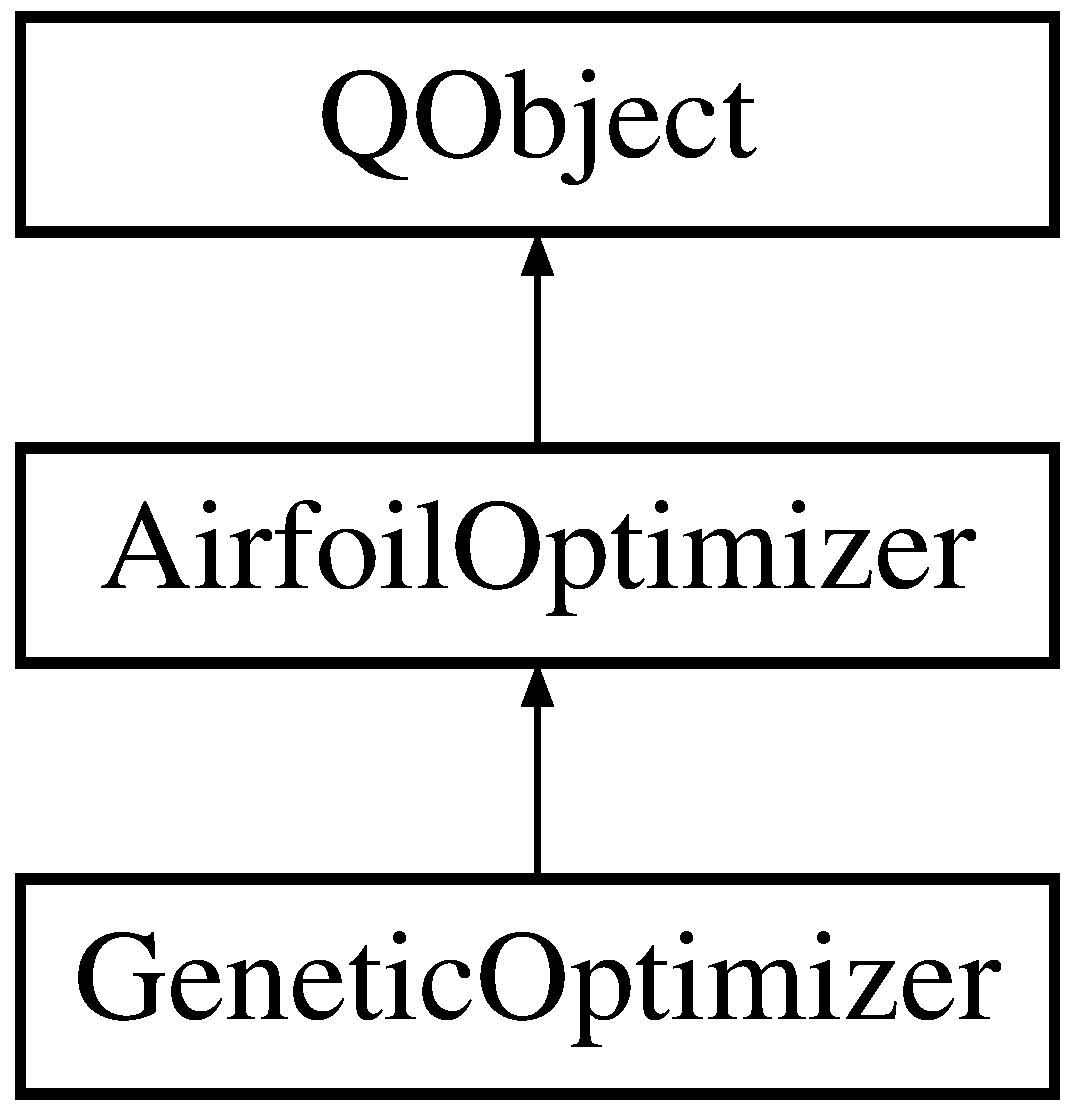
\includegraphics[height=3.000000cm]{class_genetic_optimizer}
\end{center}
\end{figure}
\subsection*{Public Types}
\begin{DoxyCompactItemize}
\item 
\mbox{\Hypertarget{class_genetic_optimizer_aa91faeb519e387199da6988e60f4a135}\label{class_genetic_optimizer_aa91faeb519e387199da6988e60f4a135}} 
enum {\bfseries G\+A\+State} \{ \newline
{\bfseries Not\+Initialized}, 
{\bfseries Initialized}, 
{\bfseries Simulation\+In\+Progress}, 
{\bfseries Generation\+Complete}, 
\newline
{\bfseries Optimization\+Complete\+Target\+Reached}, 
{\bfseries Optimization\+Complete\+Final\+Generation}
 \}
\end{DoxyCompactItemize}
\subsection*{Public Slots}
\begin{DoxyCompactItemize}
\item 
\mbox{\Hypertarget{class_genetic_optimizer_ad7fcac7f513d98f81eb91f27a5a20313}\label{class_genetic_optimizer_ad7fcac7f513d98f81eb91f27a5a20313}} 
virtual void {\bfseries simulation\+Batch\+Complete} ()
\item 
\mbox{\Hypertarget{class_genetic_optimizer_ab8fc3a1363e8cc3eb2259354ee0d689a}\label{class_genetic_optimizer_ab8fc3a1363e8cc3eb2259354ee0d689a}} 
void {\bfseries request\+Stop} ()
\end{DoxyCompactItemize}
\subsection*{Signals}
\begin{DoxyCompactItemize}
\item 
\mbox{\Hypertarget{class_genetic_optimizer_ad51ae7c1b9048c2d9df23269ac9281c8}\label{class_genetic_optimizer_ad51ae7c1b9048c2d9df23269ac9281c8}} 
void {\bfseries optimization\+Finished} ()
\item 
\mbox{\Hypertarget{class_genetic_optimizer_ab01f9fc4d56f6eccc80b2ed61ca91c0f}\label{class_genetic_optimizer_ab01f9fc4d56f6eccc80b2ed61ca91c0f}} 
void {\bfseries new\+Generation\+Generated} ()
\end{DoxyCompactItemize}
\subsection*{Public Member Functions}
\begin{DoxyCompactItemize}
\item 
\mbox{\Hypertarget{class_genetic_optimizer_a64d3d782d76c1baad7e3abd37cf376ad}\label{class_genetic_optimizer_a64d3d782d76c1baad7e3abd37cf376ad}} 
{\bfseries Genetic\+Optimizer} (\hyperlink{struct_config_1_1_simulation_params}{Config\+::\+Simulation\+Params} \&params, \hyperlink{struct_config_1_1_optimizer_params}{Config\+::\+Optimizer\+Params} \&opt\+Params)
\item 
\mbox{\Hypertarget{class_genetic_optimizer_a56ed2a002152fa57bec6596c1fbf220f}\label{class_genetic_optimizer_a56ed2a002152fa57bec6596c1fbf220f}} 
virtual void {\bfseries initialize} (\hyperlink{class_geometry}{Geometry} \&geom)
\item 
\mbox{\Hypertarget{class_genetic_optimizer_ac3350b35f1b7072ec75aef879d74d125}\label{class_genetic_optimizer_ac3350b35f1b7072ec75aef879d74d125}} 
void {\bfseries run\+Genetic\+Algorithm} ()
\item 
\mbox{\Hypertarget{class_genetic_optimizer_a33817c3a5cf8f9590a0054636af4510b}\label{class_genetic_optimizer_a33817c3a5cf8f9590a0054636af4510b}} 
G\+A\+State {\bfseries get\+State} ()
\item 
\mbox{\Hypertarget{class_genetic_optimizer_adb9c71703b5e2cb13bcb8c3c4b49b743}\label{class_genetic_optimizer_adb9c71703b5e2cb13bcb8c3c4b49b743}} 
virtual void {\bfseries optimize\+Step} ()
\item 
\mbox{\Hypertarget{class_genetic_optimizer_afbce0360126b8cb9f3e242d3bbc02422}\label{class_genetic_optimizer_afbce0360126b8cb9f3e242d3bbc02422}} 
virtual \hyperlink{class_geometry}{Geometry} const {\bfseries get\+Top\+Geometry} ()
\item 
\mbox{\Hypertarget{class_genetic_optimizer_a8d9aea6ca935024e3c5ecbc10b10c2a2}\label{class_genetic_optimizer_a8d9aea6ca935024e3c5ecbc10b10c2a2}} 
virtual double const {\bfseries get\+Progress} ()
\item 
\mbox{\Hypertarget{class_genetic_optimizer_a1db42893114197a9959fa5f7ac0176ae}\label{class_genetic_optimizer_a1db42893114197a9959fa5f7ac0176ae}} 
\hyperlink{struct_aviation_profile_parameters}{Aviation\+Profile\+Parameters} {\bfseries calculate\+Basic\+Profile} (std\+::string path)
\item 
\mbox{\Hypertarget{class_genetic_optimizer_a255076a279ba7c6665b6d06fb871f620}\label{class_genetic_optimizer_a255076a279ba7c6665b6d06fb871f620}} 
std\+::vector$<$ double $>$ {\bfseries get\+VectorX} ()
\item 
\mbox{\Hypertarget{class_genetic_optimizer_a679345a9ca88eb5122f4192c4239c276}\label{class_genetic_optimizer_a679345a9ca88eb5122f4192c4239c276}} 
std\+::vector$<$ double $>$ {\bfseries get\+VectorY} ()
\item 
\mbox{\Hypertarget{class_genetic_optimizer_a096ebb1c1b1c0630516373b236c71985}\label{class_genetic_optimizer_a096ebb1c1b1c0630516373b236c71985}} 
bool {\bfseries is\+Running} ()
\end{DoxyCompactItemize}


\subsection{Detailed Description}
Class contains implementation of the genetic algorithm. 

Genetic Optimizer provides necessary objects and methods to use genetic algorithm. General usage operates on signals and slots -\/ after run\+Simulation Slot is invoked initial population is generated And simulation is handled bu \hyperlink{class_simulation_scheduler}{Simulation\+Scheduler} object 

The documentation for this class was generated from the following files\+:\begin{DoxyCompactItemize}
\item 
optimizer/genetic/\hyperlink{genetic_8h}{genetic.\+h}\item 
optimizer/genetic/genetic.\+cpp\end{DoxyCompactItemize}

\hypertarget{struct_config_1_1_optimizer_params_1_1_genetic_optimizer_params}{}\section{Config\+:\+:Optimizer\+Params\+:\+:Genetic\+Optimizer\+Params Struct Reference}
\label{struct_config_1_1_optimizer_params_1_1_genetic_optimizer_params}\index{Config\+::\+Optimizer\+Params\+::\+Genetic\+Optimizer\+Params@{Config\+::\+Optimizer\+Params\+::\+Genetic\+Optimizer\+Params}}
\subsection*{Public Attributes}
\begin{DoxyCompactItemize}
\item 
\mbox{\Hypertarget{struct_config_1_1_optimizer_params_1_1_genetic_optimizer_params_ada7fdf8f2b62bf9ec608bd89d78b5e0b}\label{struct_config_1_1_optimizer_params_1_1_genetic_optimizer_params_ada7fdf8f2b62bf9ec608bd89d78b5e0b}} 
int {\bfseries generation\+Count} = 20
\item 
\mbox{\Hypertarget{struct_config_1_1_optimizer_params_1_1_genetic_optimizer_params_a7821ecfef62928f679f15feeda39d734}\label{struct_config_1_1_optimizer_params_1_1_genetic_optimizer_params_a7821ecfef62928f679f15feeda39d734}} 
int {\bfseries population\+Size} = 100
\item 
\mbox{\Hypertarget{struct_config_1_1_optimizer_params_1_1_genetic_optimizer_params_a4bd3aca3e2ae556590d97f720c07d4fc}\label{struct_config_1_1_optimizer_params_1_1_genetic_optimizer_params_a4bd3aca3e2ae556590d97f720c07d4fc}} 
double {\bfseries mutation\+Rate} = 0.\+005
\end{DoxyCompactItemize}


The documentation for this struct was generated from the following file\+:\begin{DoxyCompactItemize}
\item 
utility/\hyperlink{config_8h}{config.\+h}\end{DoxyCompactItemize}

\hypertarget{class_genome}{}\section{Genome Class Reference}
\label{class_genome}\index{Genome@{Genome}}
\subsection*{Public Member Functions}
\begin{DoxyCompactItemize}
\item 
\hypertarget{class_genome_a2a9830ff70a104defa32311a0df1b23b}{}\label{class_genome_a2a9830ff70a104defa32311a0df1b23b} 
{\bfseries Genome} (\hyperlink{struct_airfoil_coefficients}{Airfoil\+Coefficients} coeff)
\item 
\hypertarget{class_genome_a010985b266e041f3c96174aa0e90f8fc}{}\label{class_genome_a010985b266e041f3c96174aa0e90f8fc} 
{\bfseries Genome} (unsigned char $\ast$array)
\item 
\hypertarget{class_genome_a0604b3988e6fd685f0eaffc124aed0c9}{}\label{class_genome_a0604b3988e6fd685f0eaffc124aed0c9} 
void {\bfseries Set} (\hyperlink{struct_airfoil_coefficients}{Airfoil\+Coefficients} \&coefficients)
\item 
\hypertarget{class_genome_a80747aa266026e16dfdaf1449ba5c8aa}{}\label{class_genome_a80747aa266026e16dfdaf1449ba5c8aa} 
\hyperlink{class_geometry}{Geometry} $\ast$ {\bfseries get\+Geometry} ()
\item 
\hypertarget{class_genome_a8ebe6f37306c3aa87a8d711ec778609f}{}\label{class_genome_a8ebe6f37306c3aa87a8d711ec778609f} 
void {\bfseries set\+Fitness} (double value)
\item 
\hypertarget{class_genome_a3b61a1cd0050ad1297867a0fc42736a6}{}\label{class_genome_a3b61a1cd0050ad1297867a0fc42736a6} 
double \& {\bfseries get\+Fitness} ()
\item 
\hypertarget{class_genome_a10f096f993bdecc320aebbd2ec867305}{}\label{class_genome_a10f096f993bdecc320aebbd2ec867305} 
unsigned char $\ast$ {\bfseries get\+Coefficients\+Array} ()
\item 
\hypertarget{class_genome_ac12d4227a6f8c923c7f65d760cdeac35}{}\label{class_genome_ac12d4227a6f8c923c7f65d760cdeac35} 
\hyperlink{struct_airfoil_coefficients}{Airfoil\+Coefficients} {\bfseries get\+Coefficients} ()
\item 
\hypertarget{class_genome_a8599bccee27d2594b0364f011cfe4b3f}{}\label{class_genome_a8599bccee27d2594b0364f011cfe4b3f} 
uint8\+\_\+t {\bfseries get\+Random\+Byte} ()
\item 
\hypertarget{class_genome_ad05f549a5fb6603245f6bbd303d60ec1}{}\label{class_genome_ad05f549a5fb6603245f6bbd303d60ec1} 
void {\bfseries Set} (\hyperlink{struct_binary_airfoil_coefficients}{Binary\+Airfoil\+Coefficients} \&airfoil\+Coefficients)
\item 
\hypertarget{class_genome_a390f17f811a33f34d7bcf4a61c3b9c5d}{}\label{class_genome_a390f17f811a33f34d7bcf4a61c3b9c5d} 
void {\bfseries Set} (unsigned char $\ast$array)
\item 
\hypertarget{class_genome_a4e942202f21f552157604cda9529e19d}{}\label{class_genome_a4e942202f21f552157604cda9529e19d} 
void {\bfseries Randomize} ()
\end{DoxyCompactItemize}


The documentation for this class was generated from the following files\+:\begin{DoxyCompactItemize}
\item 
optimizer/genetic/\hyperlink{genome_8h}{genome.\+h}\item 
optimizer/genetic/genome.\+cpp\end{DoxyCompactItemize}

\hypertarget{class_genome_scrambler}{}\section{Genome\+Scrambler Class Reference}
\label{class_genome_scrambler}\index{Genome\+Scrambler@{Genome\+Scrambler}}


Abstraction class for Genetic\+Scrambler objects.  




{\ttfamily \#include $<$genome\+\_\+scrambler.\+h$>$}

Inheritance diagram for Genome\+Scrambler\+:\begin{figure}[H]
\begin{center}
\leavevmode
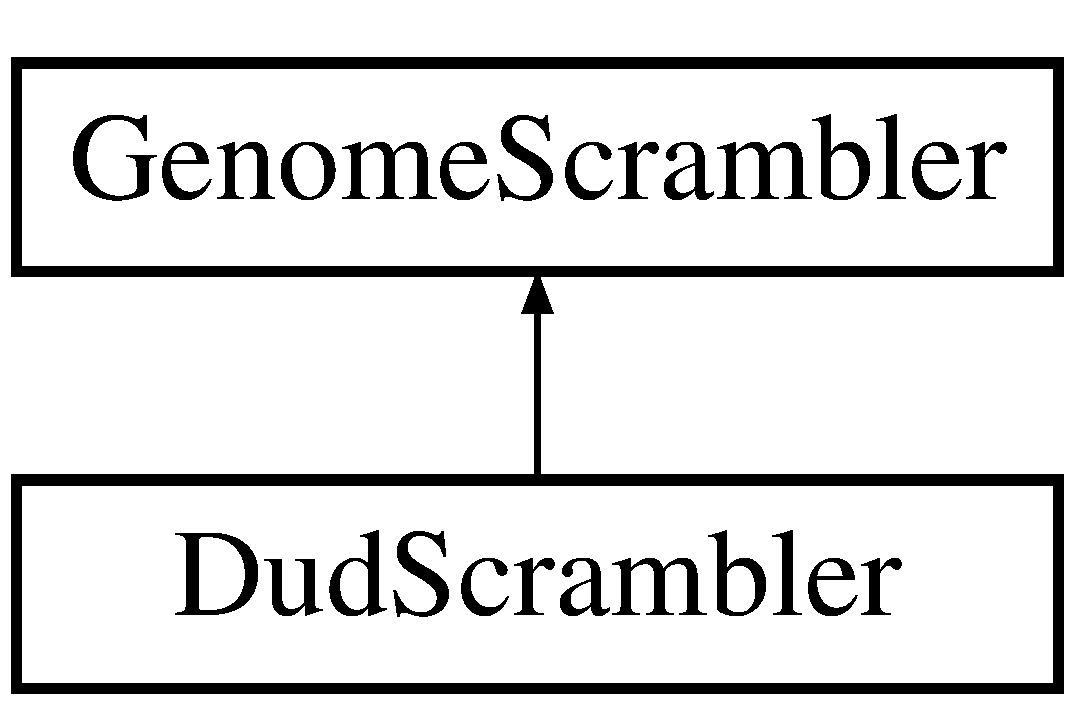
\includegraphics[height=2.000000cm]{class_genome_scrambler}
\end{center}
\end{figure}
\subsection*{Public Member Functions}
\begin{DoxyCompactItemize}
\item 
\mbox{\Hypertarget{class_genome_scrambler_a7937beaa7aa3c4a13c8c598ee0afca4a}\label{class_genome_scrambler_a7937beaa7aa3c4a13c8c598ee0afca4a}} 
virtual \hyperlink{class_genome}{Genome} $\ast$ {\bfseries mutate} (\hyperlink{class_genome}{Genome} $\ast$genome)=0
\item 
\mbox{\Hypertarget{class_genome_scrambler_a91f7407ea74f20ffc60d7af0de4e8e18}\label{class_genome_scrambler_a91f7407ea74f20ffc60d7af0de4e8e18}} 
virtual \hyperlink{class_genome}{Genome} $\ast$ {\bfseries crossover} (\hyperlink{class_genome}{Genome} $\ast$g1, \hyperlink{class_genome}{Genome} $\ast$g2)=0
\end{DoxyCompactItemize}


\subsection{Detailed Description}
Abstraction class for Genetic\+Scrambler objects. 

Genetic\+Scrambler object allows for genome crossover according to different strategies eg. single point Multi\+Point etc. 

The documentation for this class was generated from the following file\+:\begin{DoxyCompactItemize}
\item 
optimizer/genetic/\hyperlink{genome__scrambler_8h}{genome\+\_\+scrambler.\+h}\end{DoxyCompactItemize}

\hypertarget{class_geometry}{}\section{Geometry Class Reference}
\label{class_geometry}\index{Geometry@{Geometry}}


Class providing necessary attributes for geometry calculation.  




{\ttfamily \#include $<$geometry.\+h$>$}

\subsection*{Public Member Functions}
\begin{DoxyCompactItemize}
\item 
\hypertarget{class_geometry_ae86ccba6c6c851a2ff39987c7a9e842a}{}\label{class_geometry_ae86ccba6c6c851a2ff39987c7a9e842a} 
{\bfseries Geometry} (\hyperlink{struct_airfoil_coefficients}{Airfoil\+Coefficients} coeff)
\item 
\hypertarget{class_geometry_a1ef839b1538d88e53b709c69da1845f8}{}\label{class_geometry_a1ef839b1538d88e53b709c69da1845f8} 
{\bfseries Geometry} (std\+::string filename)
\item 
\hypertarget{class_geometry_a6ed211b48008ba87cc3b6744e0ea063e}{}\label{class_geometry_a6ed211b48008ba87cc3b6744e0ea063e} 
void {\bfseries Load} (std\+::string filename)
\item 
\hypertarget{class_geometry_ab4c5ee8c0ce3ef2d6df19381663ec5f3}{}\label{class_geometry_ab4c5ee8c0ce3ef2d6df19381663ec5f3} 
void {\bfseries Save} (std\+::string filename)
\item 
\hypertarget{class_geometry_acc74836e9c5bb1534fef8e7ff84ef984}{}\label{class_geometry_acc74836e9c5bb1534fef8e7ff84ef984} 
void {\bfseries Save\+Coefficients} (std\+::string filename)
\item 
\hypertarget{class_geometry_a331921e3edad630226a378bbacfce1a7}{}\label{class_geometry_a331921e3edad630226a378bbacfce1a7} 
void {\bfseries Load\+From\+Coefficients} (std\+::string filename)
\item 
\hypertarget{class_geometry_a7385b0dc9c7567efd3b37c206cfeda30}{}\label{class_geometry_a7385b0dc9c7567efd3b37c206cfeda30} 
void {\bfseries Calculate\+Coefficients} ()
\item 
\hypertarget{class_geometry_a5145d4ec1bdbc033eb510a54a6ac2eae}{}\label{class_geometry_a5145d4ec1bdbc033eb510a54a6ac2eae} 
void {\bfseries create\+New\+Geometry} (\hyperlink{struct_airfoil_coefficients}{Airfoil\+Coefficients} coeff)
\item 
\hypertarget{class_geometry_a2019d3e286dde947dd93461a63da9e65}{}\label{class_geometry_a2019d3e286dde947dd93461a63da9e65} 
void {\bfseries Normalze} ()
\item 
\hypertarget{class_geometry_a4a17704dc3342c65ee95b3352ab754ca}{}\label{class_geometry_a4a17704dc3342c65ee95b3352ab754ca} 
void {\bfseries Transform} ()
\item 
\hypertarget{class_geometry_a824e4bc80a6c08fd47d341fae8e67857}{}\label{class_geometry_a824e4bc80a6c08fd47d341fae8e67857} 
void {\bfseries regression\+Algorithm} ()
\item 
\hypertarget{class_geometry_a8db11be460efd0624647e031d6a388dc}{}\label{class_geometry_a8db11be460efd0624647e031d6a388dc} 
const \hyperlink{struct_airfoil_coefficients}{Airfoil\+Coefficients} \& {\bfseries get\+Aifroil\+Coefficients} ()
\item 
\hypertarget{class_geometry_a814f031a36718636be0491ce8618488b}{}\label{class_geometry_a814f031a36718636be0491ce8618488b} 
std\+::vector$<$ \hyperlink{class_point}{Point} $>$ {\bfseries Get\+Points} ()
\item 
\hypertarget{class_geometry_a99a0a6e2dfb453eb224cc8f01e75b7b0}{}\label{class_geometry_a99a0a6e2dfb453eb224cc8f01e75b7b0} 
const int \& {\bfseries get\+Points\+Count} ()
\item 
\hypertarget{class_geometry_a354dfd9d846b58dbd3a1090ea4227e33}{}\label{class_geometry_a354dfd9d846b58dbd3a1090ea4227e33} 
bool {\bfseries is\+Profile\+Crossed} ()
\item 
\hypertarget{class_geometry_a45255bffe9b2d5511cdb79b63532f0a1}{}\label{class_geometry_a45255bffe9b2d5511cdb79b63532f0a1} 
const \hyperlink{class_sim_results}{Sim\+Results} \& {\bfseries Get\+Results} ()
\item 
\hypertarget{class_geometry_aada258eedf595527f097faed460a5521}{}\label{class_geometry_aada258eedf595527f097faed460a5521} 
\hyperlink{class_geometry}{Geometry} \& {\bfseries operator=} (const \hyperlink{class_geometry}{Geometry} \&data)
\end{DoxyCompactItemize}
\subsection*{Friends}
\begin{DoxyCompactItemize}
\item 
\hypertarget{class_geometry_a88881bfc7b707b9bf91fd177fefa2e04}{}\label{class_geometry_a88881bfc7b707b9bf91fd177fefa2e04} 
class {\bfseries Simulation\+Handler}
\end{DoxyCompactItemize}


\subsection{Detailed Description}
Class providing necessary attributes for geometry calculation. 

This class provides loading and saving profile to file. 

The documentation for this class was generated from the following files\+:\begin{DoxyCompactItemize}
\item 
optimizer/\hyperlink{geometry_8h}{geometry.\+h}\item 
optimizer/geometry.\+cpp\end{DoxyCompactItemize}

\hypertarget{class_log_writer}{}\section{Log\+Writer Class Reference}
\label{class_log_writer}\index{Log\+Writer@{Log\+Writer}}


Class containing methods add information about current state of application.  




{\ttfamily \#include $<$log\+\_\+writer.\+h$>$}

\subsection*{Public Member Functions}
\begin{DoxyCompactItemize}
\item 
\mbox{\Hypertarget{class_log_writer_a1cedcc7f343d59239d4c9f366418d44e}\label{class_log_writer_a1cedcc7f343d59239d4c9f366418d44e}} 
bool {\bfseries initialize} (std\+::string directory\+Name)
\item 
\mbox{\Hypertarget{class_log_writer_a42c6726ace5a0b60311978edd9303a3f}\label{class_log_writer_a42c6726ace5a0b60311978edd9303a3f}} 
void {\bfseries destroy} ()
\item 
\mbox{\Hypertarget{class_log_writer_a1ce4389bff086f329383741f066f877a}\label{class_log_writer_a1ce4389bff086f329383741f066f877a}} 
void {\bfseries add\+Information\+Message} (std\+::string message)
\item 
\mbox{\Hypertarget{class_log_writer_afe4e4ca6202ee9794d78dce5dad3af79}\label{class_log_writer_afe4e4ca6202ee9794d78dce5dad3af79}} 
void {\bfseries add\+Information\+Message} (const char $\ast$message)
\item 
\mbox{\Hypertarget{class_log_writer_aa4ac503f2f74bd35f5b626f134f9315a}\label{class_log_writer_aa4ac503f2f74bd35f5b626f134f9315a}} 
void {\bfseries add\+Error\+Message} (const std\+::string \&message)
\item 
\mbox{\Hypertarget{class_log_writer_a42b4eddd43eef58d97b87580fed2b85e}\label{class_log_writer_a42b4eddd43eef58d97b87580fed2b85e}} 
void {\bfseries add\+Error\+Message} (const char $\ast$message)
\item 
\mbox{\Hypertarget{class_log_writer_a7d23476cc15635eb47f0edd9f9b74a3f}\label{class_log_writer_a7d23476cc15635eb47f0edd9f9b74a3f}} 
void {\bfseries add\+Warning\+Message} (const char $\ast$message)
\item 
\mbox{\Hypertarget{class_log_writer_a39801f380662e1bb771e1f8ee991beac}\label{class_log_writer_a39801f380662e1bb771e1f8ee991beac}} 
void {\bfseries write} (const char $\ast$message)
\end{DoxyCompactItemize}
\subsection*{Static Public Member Functions}
\begin{DoxyCompactItemize}
\item 
\mbox{\Hypertarget{class_log_writer_a112a7c453bb431bd776a1486567a516a}\label{class_log_writer_a112a7c453bb431bd776a1486567a516a}} 
static \hyperlink{class_log_writer}{Log\+Writer} \& {\bfseries get\+Instance} ()
\end{DoxyCompactItemize}


\subsection{Detailed Description}
Class containing methods add information about current state of application. 

Log writer provides to show the information on the console window and save it to the logger file. User is able to choose kind of message which he wants to show, i.\+e. information, warning or error. This class is essential for supply the data to behavior analysis of the program. 

The documentation for this class was generated from the following files\+:\begin{DoxyCompactItemize}
\item 
utility/\hyperlink{log__writer_8h}{log\+\_\+writer.\+h}\item 
utility/log\+\_\+writer.\+cpp\end{DoxyCompactItemize}

\hypertarget{struct_main_window_objects}{}\section{Main\+Window\+Objects Struct Reference}
\label{struct_main_window_objects}\index{Main\+Window\+Objects@{Main\+Window\+Objects}}
\subsection*{Public Attributes}
\begin{DoxyCompactItemize}
\item 
\hypertarget{struct_main_window_objects_ab6864383c5a6b6b5e2bf103d95ed36ce}{}\label{struct_main_window_objects_ab6864383c5a6b6b5e2bf103d95ed36ce} 
Q\+Object $\ast$ {\bfseries main\+Window}
\item 
\hypertarget{struct_main_window_objects_a005329df1cbb43b6a5efada959b08109}{}\label{struct_main_window_objects_a005329df1cbb43b6a5efada959b08109} 
\hyperlink{struct_component}{Component} {\bfseries settings\+Buttons\+Root}
\item 
\hypertarget{struct_main_window_objects_abdfa7ef5b54f46708493aa75bc8857b8}{}\label{struct_main_window_objects_abdfa7ef5b54f46708493aa75bc8857b8} 
\hyperlink{struct_component}{Component} {\bfseries base\+Parameters\+Root}
\item 
\hypertarget{struct_main_window_objects_a1c9dfd930602bbe606b2c9e23eaf1e7a}{}\label{struct_main_window_objects_a1c9dfd930602bbe606b2c9e23eaf1e7a} 
\hyperlink{struct_component}{Component} {\bfseries target\+Values\+Root}
\item 
\hypertarget{struct_main_window_objects_a9baa2379c0784fa902c370c22364d53a}{}\label{struct_main_window_objects_a9baa2379c0784fa902c370c22364d53a} 
\hyperlink{struct_component}{Component} {\bfseries fitness\+Values\+Root}
\item 
\hypertarget{struct_main_window_objects_a7377475ac90b86521112633e35a7455d}{}\label{struct_main_window_objects_a7377475ac90b86521112633e35a7455d} 
\hyperlink{struct_component}{Component} {\bfseries base\+Chart\+Frame}
\item 
\hypertarget{struct_main_window_objects_a327f6ab5bc103545a2bdf71af2709bb1}{}\label{struct_main_window_objects_a327f6ab5bc103545a2bdf71af2709bb1} 
\hyperlink{struct_component}{Component} {\bfseries optimize\+Chart\+Frame}
\item 
\hypertarget{struct_main_window_objects_a641ea5e0d975030e97f61e691754688d}{}\label{struct_main_window_objects_a641ea5e0d975030e97f61e691754688d} 
\hyperlink{struct_component}{Component} {\bfseries busy\+Indicator}
\item 
\hypertarget{struct_main_window_objects_ac937bbf4b515456afc0a02a69b864da2}{}\label{struct_main_window_objects_ac937bbf4b515456afc0a02a69b864da2} 
Q\+Object $\ast$ {\bfseries base\+Plot}
\item 
\hypertarget{struct_main_window_objects_a340c6d92e16fc0e18c084ccb31022002}{}\label{struct_main_window_objects_a340c6d92e16fc0e18c084ccb31022002} 
Q\+Object $\ast$ {\bfseries optimized\+Plot}
\item 
\hypertarget{struct_main_window_objects_ad56f352e1aef36d43dbfd98d9275a104}{}\label{struct_main_window_objects_ad56f352e1aef36d43dbfd98d9275a104} 
Q\+Object $\ast$ {\bfseries run\+Button}
\item 
\hypertarget{struct_main_window_objects_a0e90147f2b6515e2fb72d81e1a332d52}{}\label{struct_main_window_objects_a0e90147f2b6515e2fb72d81e1a332d52} 
Q\+Object $\ast$ {\bfseries stop\+Button}
\item 
\hypertarget{struct_main_window_objects_a98363267c86a7f59c7693ca5be07b3ee}{}\label{struct_main_window_objects_a98363267c86a7f59c7693ca5be07b3ee} 
std\+::vector$<$ Q\+Object $\ast$ $>$ {\bfseries settings\+Buttons}
\item 
\hypertarget{struct_main_window_objects_a1abbb394cc7ea94d4cd9d37f53e373a2}{}\label{struct_main_window_objects_a1abbb394cc7ea94d4cd9d37f53e373a2} 
std\+::vector$<$ Q\+Object $\ast$ $>$ {\bfseries base\+Parameters}
\item 
\hypertarget{struct_main_window_objects_af9867c17eb5a246afe57fef072c42950}{}\label{struct_main_window_objects_af9867c17eb5a246afe57fef072c42950} 
std\+::vector$<$ Q\+Object $\ast$ $>$ {\bfseries target\+Values}
\item 
\hypertarget{struct_main_window_objects_a0c7e32f66c72e8a5d4f59a4a1c3d2ae3}{}\label{struct_main_window_objects_a0c7e32f66c72e8a5d4f59a4a1c3d2ae3} 
std\+::vector$<$ Q\+Object $\ast$ $>$ {\bfseries fitness\+Values}
\item 
\hypertarget{struct_main_window_objects_a025c228783402e4171b6b10255e6c299}{}\label{struct_main_window_objects_a025c228783402e4171b6b10255e6c299} 
Q\+Object $\ast$ {\bfseries optimizer\+Settings}
\item 
\hypertarget{struct_main_window_objects_afefa46ef2b7b2bbb8463510cbd1fa96c}{}\label{struct_main_window_objects_afefa46ef2b7b2bbb8463510cbd1fa96c} 
const int {\bfseries buttons\+Count} = 3
\item 
\hypertarget{struct_main_window_objects_a90fb8550521905b8ff5deb3ada029bf6}{}\label{struct_main_window_objects_a90fb8550521905b8ff5deb3ada029bf6} 
const int {\bfseries parameters\+Label\+Count} = 3
\item 
\hypertarget{struct_main_window_objects_a8ecfc11bef148eccb169de602894f430}{}\label{struct_main_window_objects_a8ecfc11bef148eccb169de602894f430} 
bool {\bfseries S\+E\+T\+\_\+\+T\+A\+R\+G\+ET} = false
\item 
\hypertarget{struct_main_window_objects_afd2840313b5e375d9fc611433f881481}{}\label{struct_main_window_objects_afd2840313b5e375d9fc611433f881481} 
bool {\bfseries S\+E\+T\+\_\+\+B\+A\+SE} = false
\item 
\hypertarget{struct_main_window_objects_a33cf57580a48e05aa26084a2e885c56b}{}\label{struct_main_window_objects_a33cf57580a48e05aa26084a2e885c56b} 
bool {\bfseries R\+U\+N\+\_\+\+B\+U\+T\+T\+O\+N\+\_\+\+I\+S\+\_\+\+P\+R\+E\+S\+S\+ED} = false
\end{DoxyCompactItemize}


The documentation for this struct was generated from the following file\+:\begin{DoxyCompactItemize}
\item 
gui/\hyperlink{gui__objects_8h}{gui\+\_\+objects.\+h}\end{DoxyCompactItemize}

\hypertarget{class_model}{}\section{Model Class Reference}
\label{class_model}\index{Model@{Model}}


Class manage G\+UI and genethic algorithm.  




{\ttfamily \#include $<$model.\+h$>$}

Inheritance diagram for Model\+:\begin{figure}[H]
\begin{center}
\leavevmode
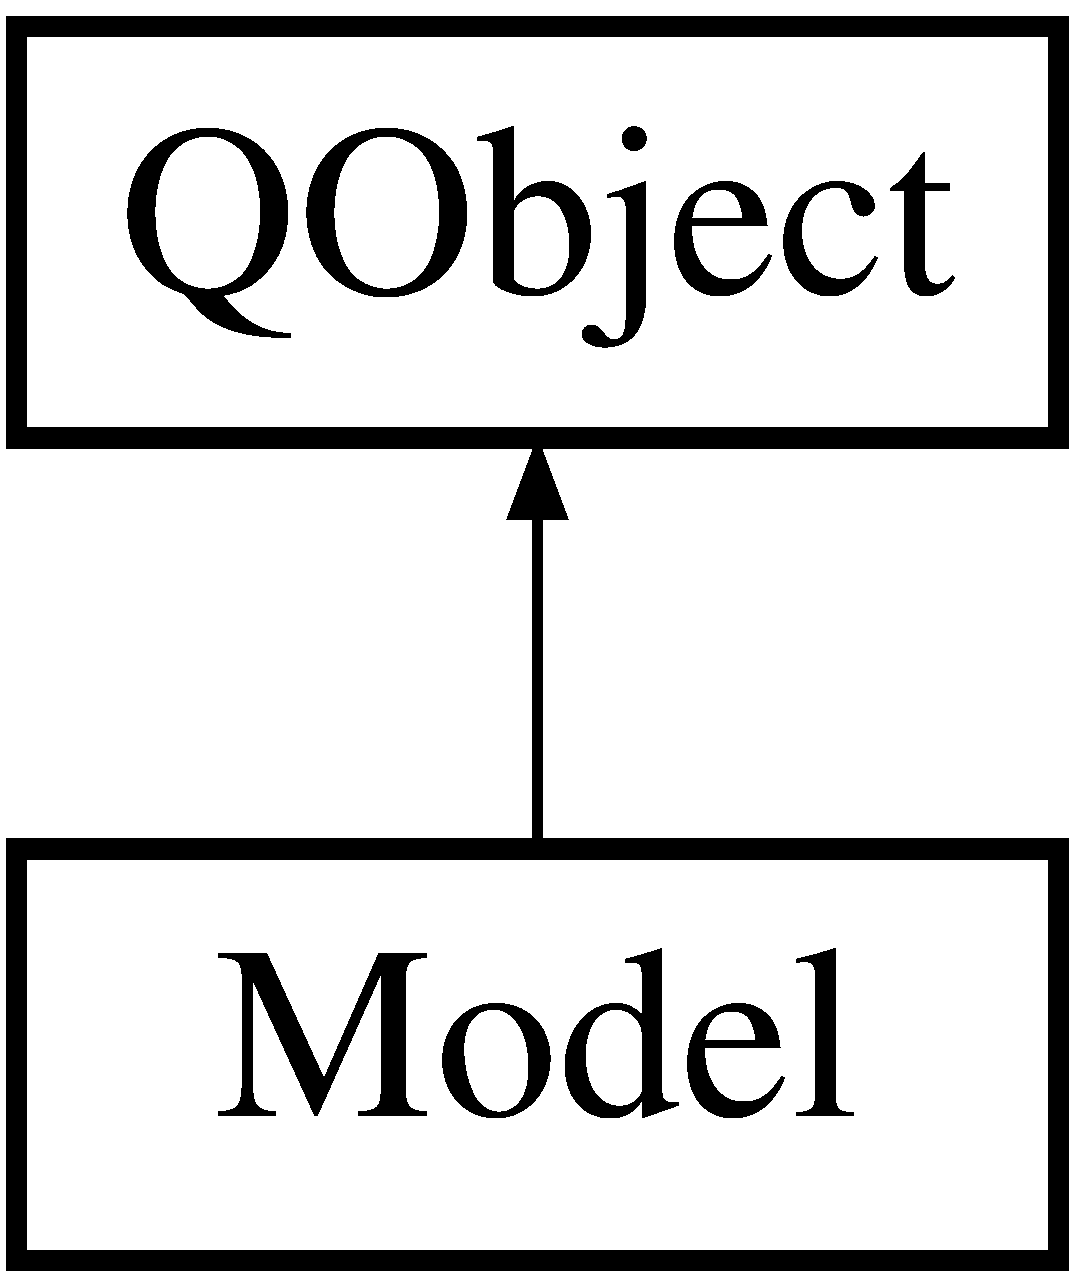
\includegraphics[height=2.000000cm]{class_model}
\end{center}
\end{figure}
\subsection*{Public Slots}
\begin{DoxyCompactItemize}
\item 
\mbox{\Hypertarget{class_model_a61c13cae7083b057b444fcf40494e8c9}\label{class_model_a61c13cae7083b057b444fcf40494e8c9}} 
void {\bfseries get\+Target\+Profile\+Values} (\hyperlink{struct_aviation_profile_parameters}{Aviation\+Profile\+Parameters} data)
\item 
\mbox{\Hypertarget{class_model_a3c060dfaec8c6d145356f6126f2859c4}\label{class_model_a3c060dfaec8c6d145356f6126f2859c4}} 
void {\bfseries calculate\+Base\+Profile\+Parameters} (std\+::string path)
\item 
\mbox{\Hypertarget{class_model_a74ab64a55f20be50aeeaf27f8c6cfea8}\label{class_model_a74ab64a55f20be50aeeaf27f8c6cfea8}} 
void {\bfseries get\+Optimized\+Geometry} ()
\item 
\mbox{\Hypertarget{class_model_a6452e846a5e560220236b7a59f1dd84b}\label{class_model_a6452e846a5e560220236b7a59f1dd84b}} 
void {\bfseries stop\+Simulation} ()
\item 
\mbox{\Hypertarget{class_model_a6fd6613a5141552a6493eb3a840cde24}\label{class_model_a6fd6613a5141552a6493eb3a840cde24}} 
void {\bfseries start\+Simulation} ()
\end{DoxyCompactItemize}
\subsection*{Signals}
\begin{DoxyCompactItemize}
\item 
\mbox{\Hypertarget{class_model_aaafc71e874110691200a3669d7e2de09}\label{class_model_aaafc71e874110691200a3669d7e2de09}} 
void {\bfseries update\+Base\+Chart} (const std\+::vector$<$ double $>$ \&dataX, const std\+::vector$<$ double $>$ \&dataY)
\item 
\mbox{\Hypertarget{class_model_a75de03d87bf729d8204c303d1b465db6}\label{class_model_a75de03d87bf729d8204c303d1b465db6}} 
void {\bfseries update\+Optimized\+Chart} (const std\+::vector$<$ double $>$ \&dataX, const std\+::vector$<$ double $>$ \&dataY)
\item 
\mbox{\Hypertarget{class_model_a054ed50fcc64d1d202e9e12acb1654b1}\label{class_model_a054ed50fcc64d1d202e9e12acb1654b1}} 
void {\bfseries update\+Genetic\+Chart} (const std\+::vector$<$ double $>$ \&dataX, const std\+::vector$<$ double $>$ \&dataY)
\item 
\mbox{\Hypertarget{class_model_afbde50de7b8ca6bdeeb169605fa144f4}\label{class_model_afbde50de7b8ca6bdeeb169605fa144f4}} 
void {\bfseries set\+Fitness\+Parameters} (\hyperlink{struct_aviation_profile_parameters}{Aviation\+Profile\+Parameters} data)
\item 
\mbox{\Hypertarget{class_model_a5dd37391b4c2efe80fa29ab7f84157aa}\label{class_model_a5dd37391b4c2efe80fa29ab7f84157aa}} 
void {\bfseries set\+Basic\+Profile\+Parameters} (\hyperlink{struct_aviation_profile_parameters}{Aviation\+Profile\+Parameters} data)
\end{DoxyCompactItemize}


\subsection{Detailed Description}
Class manage G\+UI and genethic algorithm. 

Get data from user interface and redirect it to genethic algorithm. 

The documentation for this class was generated from the following files\+:\begin{DoxyCompactItemize}
\item 
model/\hyperlink{model_8h}{model.\+h}\item 
model/model.\+cpp\end{DoxyCompactItemize}

\hypertarget{struct_config_1_1_optimizer_params}{}\section{Config\+:\+:Optimizer\+Params Struct Reference}
\label{struct_config_1_1_optimizer_params}\index{Config\+::\+Optimizer\+Params@{Config\+::\+Optimizer\+Params}}
\subsection*{Classes}
\begin{DoxyCompactItemize}
\item 
struct \hyperlink{struct_config_1_1_optimizer_params_1_1_fitness}{Fitness}
\item 
struct \hyperlink{struct_config_1_1_optimizer_params_1_1_genetic_optimizer_params}{Genetic\+Optimizer\+Params}
\end{DoxyCompactItemize}
\subsection*{Public Types}
\begin{DoxyCompactItemize}
\item 
\mbox{\Hypertarget{struct_config_1_1_optimizer_params_a5af58e4f3cf954086eaf5e8b43412a23}\label{struct_config_1_1_optimizer_params_a5af58e4f3cf954086eaf5e8b43412a23}} 
enum {\bfseries Optimizer\+Type} \{ {\bfseries Genetic}
 \}
\end{DoxyCompactItemize}
\subsection*{Public Attributes}
\begin{DoxyCompactItemize}
\item 
\mbox{\Hypertarget{struct_config_1_1_optimizer_params_a556b51c730b3f5b3640de00247cb9148}\label{struct_config_1_1_optimizer_params_a556b51c730b3f5b3640de00247cb9148}} 
\hyperlink{struct_config_1_1_optimizer_params_1_1_fitness}{Fitness} {\bfseries fitness}
\item 
\mbox{\Hypertarget{struct_config_1_1_optimizer_params_a3f676c6d7b5e15253620c16859663b2c}\label{struct_config_1_1_optimizer_params_a3f676c6d7b5e15253620c16859663b2c}} 
Optimizer\+Type {\bfseries optimizer\+Type} = Genetic
\item 
\mbox{\Hypertarget{struct_config_1_1_optimizer_params_a76fac8f9bcac64ee0a1694faec04d084}\label{struct_config_1_1_optimizer_params_a76fac8f9bcac64ee0a1694faec04d084}} 
\hyperlink{struct_config_1_1_optimizer_params_1_1_genetic_optimizer_params}{Genetic\+Optimizer\+Params} {\bfseries genetic\+Optimizer}
\item 
\mbox{\Hypertarget{struct_config_1_1_optimizer_params_a9d96a4d78bec250c3742eb5dc3ada304}\label{struct_config_1_1_optimizer_params_a9d96a4d78bec250c3742eb5dc3ada304}} 
\hyperlink{struct_config_1_1_simulation_params}{Simulation\+Params} {\bfseries simulation}
\end{DoxyCompactItemize}


The documentation for this struct was generated from the following file\+:\begin{DoxyCompactItemize}
\item 
utility/\hyperlink{config_8h}{config.\+h}\end{DoxyCompactItemize}

\hypertarget{struct_plot}{}\section{Plot Struct Reference}
\label{struct_plot}\index{Plot@{Plot}}
\subsection*{Public Attributes}
\begin{DoxyCompactItemize}
\item 
\hypertarget{struct_plot_aef96b91eab77fc58e9d337c97bf16d0b}{}\label{struct_plot_aef96b91eab77fc58e9d337c97bf16d0b} 
Q\+Object $\ast$ {\bfseries plot\+Window}
\item 
\hypertarget{struct_plot_a22a2aea9b9cf01dcfeaf43deda9cc6e3}{}\label{struct_plot_a22a2aea9b9cf01dcfeaf43deda9cc6e3} 
Q\+Object $\ast$ {\bfseries plot\+Frame}
\item 
\hypertarget{struct_plot_a9c90096944ddbb2cfeddd9cf17f6d483}{}\label{struct_plot_a9c90096944ddbb2cfeddd9cf17f6d483} 
Q\+Object $\ast$ {\bfseries plot}
\end{DoxyCompactItemize}


The documentation for this struct was generated from the following file\+:\begin{DoxyCompactItemize}
\item 
gui/\hyperlink{gui__objects_8h}{gui\+\_\+objects.\+h}\end{DoxyCompactItemize}

\hypertarget{class_plot_dialog}{}\section{Plot\+Dialog Class Reference}
\label{class_plot_dialog}\index{Plot\+Dialog@{Plot\+Dialog}}


Class provides drawing chart in external dialog.  




{\ttfamily \#include $<$plot\+\_\+dialog.\+h$>$}

Inheritance diagram for Plot\+Dialog\+:\begin{figure}[H]
\begin{center}
\leavevmode
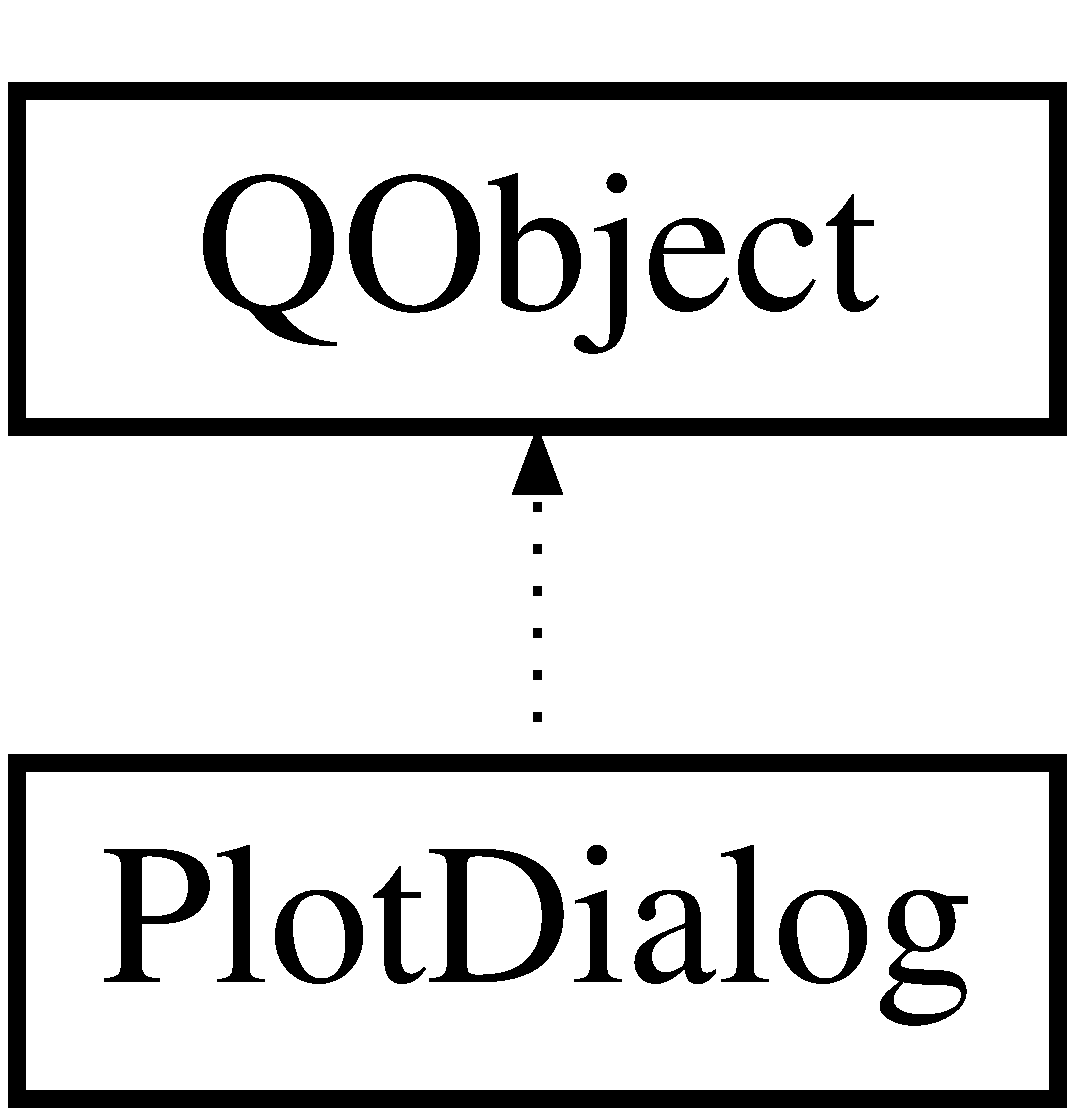
\includegraphics[height=2.000000cm]{class_plot_dialog}
\end{center}
\end{figure}
\subsection*{Public Member Functions}
\begin{DoxyCompactItemize}
\item 
\mbox{\Hypertarget{class_plot_dialog_ae5fb95c5336b5dd2267101dd181989a5}\label{class_plot_dialog_ae5fb95c5336b5dd2267101dd181989a5}} 
void {\bfseries initialize} (Q\+Qml\+Application\+Engine \&engine)
\item 
\mbox{\Hypertarget{class_plot_dialog_a7b5d5b476275028bf4186e737d50ebbe}\label{class_plot_dialog_a7b5d5b476275028bf4186e737d50ebbe}} 
void {\bfseries show\+Dialog} ()
\item 
\mbox{\Hypertarget{class_plot_dialog_a5bb43876e8c339604c4827d536a54726}\label{class_plot_dialog_a5bb43876e8c339604c4827d536a54726}} 
void {\bfseries draw\+Chart} (const std\+::vector$<$ double $>$ \&data\+X\+\_\+, const std\+::vector$<$ double $>$ \&data\+Y\+\_\+)
\item 
\mbox{\Hypertarget{class_plot_dialog_aeffbb53cffcdb443a0395a147d2b684b}\label{class_plot_dialog_aeffbb53cffcdb443a0395a147d2b684b}} 
void {\bfseries clear} ()
\end{DoxyCompactItemize}


\subsection{Detailed Description}
Class provides drawing chart in external dialog. 

The documentation for this class was generated from the following files\+:\begin{DoxyCompactItemize}
\item 
gui/\hyperlink{plot__dialog_8h}{plot\+\_\+dialog.\+h}\item 
gui/plot\+\_\+dialog.\+cpp\end{DoxyCompactItemize}

\hypertarget{class_point}{}\section{Point Class Reference}
\label{class_point}\index{Point@{Point}}
\subsection*{Public Member Functions}
\begin{DoxyCompactItemize}
\item 
\hypertarget{class_point_a2a0253a42cde677081c10532edcfc65f}{}\label{class_point_a2a0253a42cde677081c10532edcfc65f} 
{\bfseries Point} (double xin, double yin)
\end{DoxyCompactItemize}
\subsection*{Public Attributes}
\begin{DoxyCompactItemize}
\item 
\hypertarget{class_point_ab99c56589bc8ad5fa5071387110a5bc7}{}\label{class_point_ab99c56589bc8ad5fa5071387110a5bc7} 
double {\bfseries x}
\item 
\hypertarget{class_point_afa38be143ae800e6ad69ce8ed4df62d8}{}\label{class_point_afa38be143ae800e6ad69ce8ed4df62d8} 
double {\bfseries y}
\end{DoxyCompactItemize}


The documentation for this class was generated from the following file\+:\begin{DoxyCompactItemize}
\item 
optimizer/\hyperlink{geometry__structures_8h}{geometry\+\_\+structures.\+h}\end{DoxyCompactItemize}

\hypertarget{struct_sim_results_1_1_polar_point}{}\section{Sim\+Results\+:\+:Polar\+Point Struct Reference}
\label{struct_sim_results_1_1_polar_point}\index{Sim\+Results\+::\+Polar\+Point@{Sim\+Results\+::\+Polar\+Point}}
\subsection*{Public Attributes}
\begin{DoxyCompactItemize}
\item 
\mbox{\Hypertarget{struct_sim_results_1_1_polar_point_a42f2c76e058f9f40c22be5194e30ed9b}\label{struct_sim_results_1_1_polar_point_a42f2c76e058f9f40c22be5194e30ed9b}} 
double {\bfseries alfa}
\item 
\mbox{\Hypertarget{struct_sim_results_1_1_polar_point_ad3fd235e4e540eb0d1ecb0cdade8054b}\label{struct_sim_results_1_1_polar_point_ad3fd235e4e540eb0d1ecb0cdade8054b}} 
double {\bfseries param}
\end{DoxyCompactItemize}


The documentation for this struct was generated from the following file\+:\begin{DoxyCompactItemize}
\item 
optimizer/\hyperlink{simulation__results_8h}{simulation\+\_\+results.\+h}\end{DoxyCompactItemize}

\hypertarget{class_q_simulation_proxy}{}\section{Q\+Simulation\+Proxy Class Reference}
\label{class_q_simulation_proxy}\index{Q\+Simulation\+Proxy@{Q\+Simulation\+Proxy}}


IO stream interface using QT Qprocess A\+PI.  




{\ttfamily \#include $<$qsimulation.\+h$>$}

Inheritance diagram for Q\+Simulation\+Proxy\+:\begin{figure}[H]
\begin{center}
\leavevmode
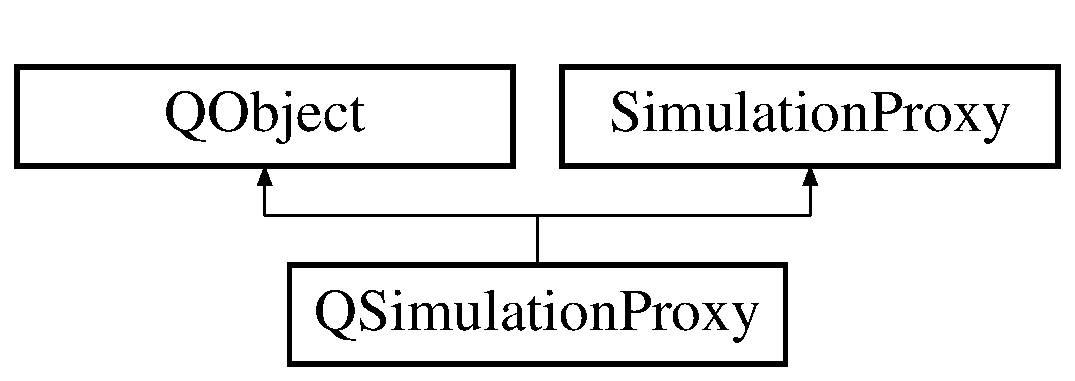
\includegraphics[height=2.000000cm]{class_q_simulation_proxy}
\end{center}
\end{figure}
\subsection*{Public Types}
\begin{DoxyCompactItemize}
\item 
\hypertarget{class_q_simulation_proxy_a85e46e407b5003b30885178dbf01edfb}{}\label{class_q_simulation_proxy_a85e46e407b5003b30885178dbf01edfb} 
typedef std\+::chrono\+::steady\+\_\+clock\+::time\+\_\+point {\bfseries Time\+Point}
\item 
\hypertarget{class_q_simulation_proxy_a4dc47dcbf523e98cb6290707e88297dc}{}\label{class_q_simulation_proxy_a4dc47dcbf523e98cb6290707e88297dc} 
typedef std\+::chrono\+::steady\+\_\+clock {\bfseries Clock}
\end{DoxyCompactItemize}
\subsection*{Public Member Functions}
\begin{DoxyCompactItemize}
\item 
\hypertarget{class_q_simulation_proxy_a10836d0c32979096e2f717fc52fe9cfe}{}\label{class_q_simulation_proxy_a10836d0c32979096e2f717fc52fe9cfe} 
{\bfseries Q\+Simulation\+Proxy} (const \hyperlink{struct_config_1_1_simulation_params}{Config\+::\+Simulation\+Params} \&params, Q\+Object $\ast$parent=0)
\item 
\hypertarget{class_q_simulation_proxy_ac2ec0d6fcbb367a09215fa74a0e07097}{}\label{class_q_simulation_proxy_ac2ec0d6fcbb367a09215fa74a0e07097} 
virtual void {\bfseries Add\+Command} (std\+::string command) override
\item 
\hypertarget{class_q_simulation_proxy_accbf718d10c3d97bc969d40041079a2e}{}\label{class_q_simulation_proxy_accbf718d10c3d97bc969d40041079a2e} 
virtual void {\bfseries Run} () override
\item 
\hypertarget{class_q_simulation_proxy_aef1ca5b3fa662109c5f45e0b277df2db}{}\label{class_q_simulation_proxy_aef1ca5b3fa662109c5f45e0b277df2db} 
virtual void {\bfseries Terminate} () override
\item 
\hypertarget{class_q_simulation_proxy_aae992d752c79bca078612afb918a0683}{}\label{class_q_simulation_proxy_aae992d752c79bca078612afb918a0683} 
virtual Status {\bfseries Poll\+Status} () override
\item 
\hypertarget{class_q_simulation_proxy_ab8be04fedafdc3f9924703dafb68611b}{}\label{class_q_simulation_proxy_ab8be04fedafdc3f9924703dafb68611b} 
virtual std\+::string const {\bfseries Get\+Program\+Output} () override
\item 
\hypertarget{class_q_simulation_proxy_a51336e36115ed18a9b78aba8fdabe4db}{}\label{class_q_simulation_proxy_a51336e36115ed18a9b78aba8fdabe4db} 
virtual std\+::string const {\bfseries Get\+Exe\+Path} () override
\end{DoxyCompactItemize}


\subsection{Detailed Description}
IO stream interface using QT Qprocess A\+PI. 

The documentation for this class was generated from the following files\+:\begin{DoxyCompactItemize}
\item 
xfoil/\hyperlink{qsimulation_8h}{qsimulation.\+h}\item 
xfoil/qsimulation.\+cpp\end{DoxyCompactItemize}

\hypertarget{struct_sim_results_1_1_result_entry}{}\section{Sim\+Results\+:\+:Result\+Entry Struct Reference}
\label{struct_sim_results_1_1_result_entry}\index{Sim\+Results\+::\+Result\+Entry@{Sim\+Results\+::\+Result\+Entry}}


Class containing simulation results from xfoil Structure for storing simulation results from xfoil panel optimizer.  




{\ttfamily \#include $<$simulation\+\_\+results.\+h$>$}

\subsection*{Public Attributes}
\begin{DoxyCompactItemize}
\item 
float \hyperlink{struct_sim_results_1_1_result_entry_aeebdc22ea1d6227bc7bb734b772cdde4}{alfa}
\item 
float \hyperlink{struct_sim_results_1_1_result_entry_afab2cac74d2206faeb9a590eb9accf65}{cl}
\item 
\mbox{\Hypertarget{struct_sim_results_1_1_result_entry_a2eb610ab85a129e1b4dd1a7c23780a9b}\label{struct_sim_results_1_1_result_entry_a2eb610ab85a129e1b4dd1a7c23780a9b}} 
float {\bfseries cd}
\item 
float \hyperlink{struct_sim_results_1_1_result_entry_a908f88a569d107f81ea9b2182e4046be}{cdp}
\item 
float \hyperlink{struct_sim_results_1_1_result_entry_af2e79ccca64b400a53ff4c05319150da}{cm}
\item 
float \hyperlink{struct_sim_results_1_1_result_entry_a78de4c9c6ccbf398eb0cdc6d4a85e479}{xtr\+\_\+top}
\item 
float \hyperlink{struct_sim_results_1_1_result_entry_afc790d71044cb3d5f0fa9a02521c0b21}{xtr\+\_\+bottom}
\end{DoxyCompactItemize}


\subsection{Detailed Description}
Class containing simulation results from xfoil Structure for storing simulation results from xfoil panel optimizer. 

This class calculate airfoil\textquotesingle{}s parameters based on the outputs from xfoil simulation. 

\subsection{Member Data Documentation}
\mbox{\Hypertarget{struct_sim_results_1_1_result_entry_aeebdc22ea1d6227bc7bb734b772cdde4}\label{struct_sim_results_1_1_result_entry_aeebdc22ea1d6227bc7bb734b772cdde4}} 
\index{Sim\+Results\+::\+Result\+Entry@{Sim\+Results\+::\+Result\+Entry}!alfa@{alfa}}
\index{alfa@{alfa}!Sim\+Results\+::\+Result\+Entry@{Sim\+Results\+::\+Result\+Entry}}
\subsubsection{\texorpdfstring{alfa}{alfa}}
{\footnotesize\ttfamily Sim\+Results\+::\+Result\+Entry\+::alfa}

airfoil angle of attack for the calculation \mbox{\Hypertarget{struct_sim_results_1_1_result_entry_a908f88a569d107f81ea9b2182e4046be}\label{struct_sim_results_1_1_result_entry_a908f88a569d107f81ea9b2182e4046be}} 
\index{Sim\+Results\+::\+Result\+Entry@{Sim\+Results\+::\+Result\+Entry}!cdp@{cdp}}
\index{cdp@{cdp}!Sim\+Results\+::\+Result\+Entry@{Sim\+Results\+::\+Result\+Entry}}
\subsubsection{\texorpdfstring{cdp}{cdp}}
{\footnotesize\ttfamily Sim\+Results\+::\+Result\+Entry\+::cdp}

Pressure coefficient \mbox{\Hypertarget{struct_sim_results_1_1_result_entry_afab2cac74d2206faeb9a590eb9accf65}\label{struct_sim_results_1_1_result_entry_afab2cac74d2206faeb9a590eb9accf65}} 
\index{Sim\+Results\+::\+Result\+Entry@{Sim\+Results\+::\+Result\+Entry}!cl@{cl}}
\index{cl@{cl}!Sim\+Results\+::\+Result\+Entry@{Sim\+Results\+::\+Result\+Entry}}
\subsubsection{\texorpdfstring{cl}{cl}}
{\footnotesize\ttfamily Sim\+Results\+::\+Result\+Entry\+::cl}

Lift coefficient \mbox{\Hypertarget{struct_sim_results_1_1_result_entry_af2e79ccca64b400a53ff4c05319150da}\label{struct_sim_results_1_1_result_entry_af2e79ccca64b400a53ff4c05319150da}} 
\index{Sim\+Results\+::\+Result\+Entry@{Sim\+Results\+::\+Result\+Entry}!cm@{cm}}
\index{cm@{cm}!Sim\+Results\+::\+Result\+Entry@{Sim\+Results\+::\+Result\+Entry}}
\subsubsection{\texorpdfstring{cm}{cm}}
{\footnotesize\ttfamily Sim\+Results\+::\+Result\+Entry\+::cm}

Tirque coefficient \mbox{\Hypertarget{struct_sim_results_1_1_result_entry_afc790d71044cb3d5f0fa9a02521c0b21}\label{struct_sim_results_1_1_result_entry_afc790d71044cb3d5f0fa9a02521c0b21}} 
\index{Sim\+Results\+::\+Result\+Entry@{Sim\+Results\+::\+Result\+Entry}!xtr\+\_\+bottom@{xtr\+\_\+bottom}}
\index{xtr\+\_\+bottom@{xtr\+\_\+bottom}!Sim\+Results\+::\+Result\+Entry@{Sim\+Results\+::\+Result\+Entry}}
\subsubsection{\texorpdfstring{xtr\+\_\+bottom}{xtr\_bottom}}
{\footnotesize\ttfamily Sim\+Results\+::\+Result\+Entry\+::xtr\+\_\+bottom}

Bottom transition point \begin{DoxyAuthor}{Author}
Jakub Polaczek \& Hubert Buczyński 
\end{DoxyAuthor}
\begin{DoxyDate}{Date}
05/06/2017 
\end{DoxyDate}
\mbox{\Hypertarget{struct_sim_results_1_1_result_entry_a78de4c9c6ccbf398eb0cdc6d4a85e479}\label{struct_sim_results_1_1_result_entry_a78de4c9c6ccbf398eb0cdc6d4a85e479}} 
\index{Sim\+Results\+::\+Result\+Entry@{Sim\+Results\+::\+Result\+Entry}!xtr\+\_\+top@{xtr\+\_\+top}}
\index{xtr\+\_\+top@{xtr\+\_\+top}!Sim\+Results\+::\+Result\+Entry@{Sim\+Results\+::\+Result\+Entry}}
\subsubsection{\texorpdfstring{xtr\+\_\+top}{xtr\_top}}
{\footnotesize\ttfamily Sim\+Results\+::\+Result\+Entry\+::xtr\+\_\+top}

Top transition point 

The documentation for this struct was generated from the following file\+:\begin{DoxyCompactItemize}
\item 
optimizer/\hyperlink{simulation__results_8h}{simulation\+\_\+results.\+h}\end{DoxyCompactItemize}

\hypertarget{class_scheduler_worker}{}\section{Scheduler\+Worker Class Reference}
\label{class_scheduler_worker}\index{Scheduler\+Worker@{Scheduler\+Worker}}


Class controlling execution of multiple handlers to be deployed in a dedicated thread.  




{\ttfamily \#include $<$simulation.\+h$>$}

Inheritance diagram for Scheduler\+Worker\+:\begin{figure}[H]
\begin{center}
\leavevmode
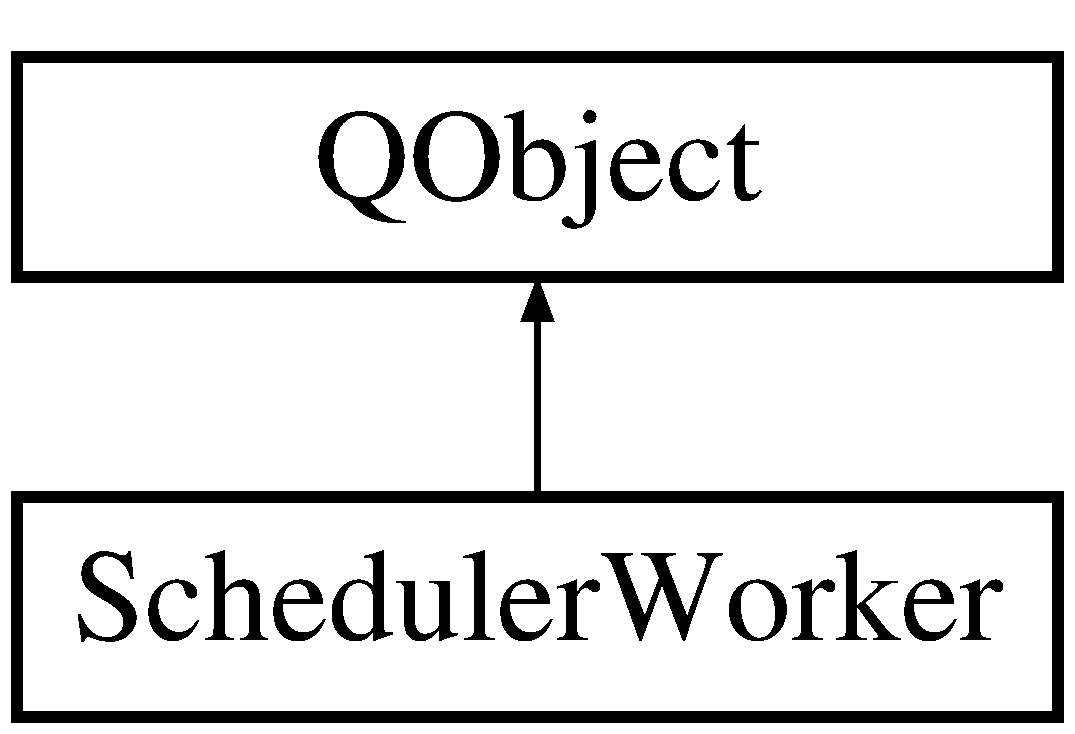
\includegraphics[height=2.000000cm]{class_scheduler_worker}
\end{center}
\end{figure}
\subsection*{Public Slots}
\begin{DoxyCompactItemize}
\item 
\mbox{\Hypertarget{class_scheduler_worker_ac5b2e3ffa0470416221e3ec07956a628}\label{class_scheduler_worker_ac5b2e3ffa0470416221e3ec07956a628}} 
void {\bfseries stop} ()
\item 
\mbox{\Hypertarget{class_scheduler_worker_ae17d3b4fd5068714a32b8be97a7ecac1}\label{class_scheduler_worker_ae17d3b4fd5068714a32b8be97a7ecac1}} 
void {\bfseries start} ()
\item 
\mbox{\Hypertarget{class_scheduler_worker_a15b321a2369b6ccfe7af4351ed4d1960}\label{class_scheduler_worker_a15b321a2369b6ccfe7af4351ed4d1960}} 
void {\bfseries add\+Task} (\hyperlink{struct_task}{Task} task)
\item 
\mbox{\Hypertarget{class_scheduler_worker_a35a536a33b478e22f28dd508d6eb3242}\label{class_scheduler_worker_a35a536a33b478e22f28dd508d6eb3242}} 
void {\bfseries process} ()
\item 
\mbox{\Hypertarget{class_scheduler_worker_a93bcfd25dea100ac89372fc14710c86e}\label{class_scheduler_worker_a93bcfd25dea100ac89372fc14710c86e}} 
bool {\bfseries Is\+Tasks\+Finished} ()
\end{DoxyCompactItemize}
\subsection*{Signals}
\begin{DoxyCompactItemize}
\item 
\mbox{\Hypertarget{class_scheduler_worker_a2fd120b582cb00372117bbd5b1f2238d}\label{class_scheduler_worker_a2fd120b582cb00372117bbd5b1f2238d}} 
void {\bfseries finished\+Work} ()
\item 
\mbox{\Hypertarget{class_scheduler_worker_a6258fd2861a3ce7798436f017b5de36a}\label{class_scheduler_worker_a6258fd2861a3ce7798436f017b5de36a}} 
void {\bfseries update\+Idle\+State} (bool state)
\item 
\mbox{\Hypertarget{class_scheduler_worker_a12e2df7be830c191c58afe3aead3b942}\label{class_scheduler_worker_a12e2df7be830c191c58afe3aead3b942}} 
void {\bfseries error} (Q\+String str)
\end{DoxyCompactItemize}
\subsection*{Public Member Functions}
\begin{DoxyCompactItemize}
\item 
\mbox{\Hypertarget{class_scheduler_worker_abbce89dd767e79876256848966f38dda}\label{class_scheduler_worker_abbce89dd767e79876256848966f38dda}} 
{\bfseries Scheduler\+Worker} (std\+::queue$<$ \hyperlink{struct_task}{Task} $>$ \&task\+Queue, Q\+Mutex \&mutex, \hyperlink{struct_config_1_1_simulation_params}{Config\+::\+Simulation\+Params} params, Q\+Object $\ast$parent=0)
\end{DoxyCompactItemize}


\subsection{Detailed Description}
Class controlling execution of multiple handlers to be deployed in a dedicated thread. 

Clas runns in a separate thread and controls multiple simulation handlers execution (according to thread count parameter) 

The documentation for this class was generated from the following files\+:\begin{DoxyCompactItemize}
\item 
xfoil/\hyperlink{simulation_8h}{simulation.\+h}\item 
xfoil/simulation.\+cpp\end{DoxyCompactItemize}

\hypertarget{class_settings_dialog}{}\section{Settings\+Dialog Class Reference}
\label{class_settings_dialog}\index{Settings\+Dialog@{Settings\+Dialog}}


The class takes care of genetic algorithm\textquotesingle{}s settings obtain from user.  




{\ttfamily \#include $<$settings\+\_\+dialog.\+h$>$}

Inheritance diagram for Settings\+Dialog\+:\begin{figure}[H]
\begin{center}
\leavevmode
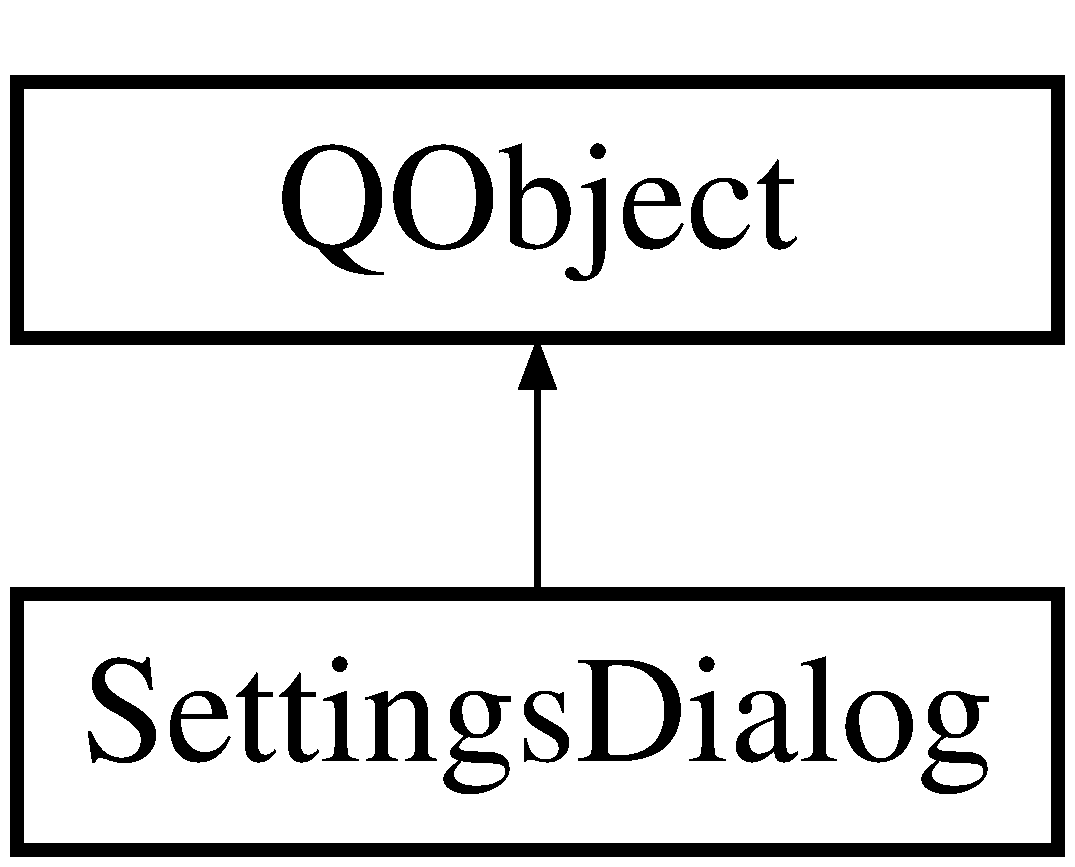
\includegraphics[height=2.000000cm]{class_settings_dialog}
\end{center}
\end{figure}
\subsection*{Public Slots}
\begin{DoxyCompactItemize}
\item 
\hypertarget{class_settings_dialog_a39b1536560a0eeb6fab732deee884f6d}{}\label{class_settings_dialog_a39b1536560a0eeb6fab732deee884f6d} 
void {\bfseries buttons\+Clicked} (Q\+String name)
\end{DoxyCompactItemize}
\subsection*{Signals}
\begin{DoxyCompactItemize}
\item 
\hypertarget{class_settings_dialog_a324625fc61d22dc18cc7f1ba15ebdb9a}{}\label{class_settings_dialog_a324625fc61d22dc18cc7f1ba15ebdb9a} 
void {\bfseries redirect\+Optimizer\+Parameters} ()
\end{DoxyCompactItemize}
\subsection*{Public Member Functions}
\begin{DoxyCompactItemize}
\item 
\hypertarget{class_settings_dialog_acf8060ba9a873b7c6b1ccdd167fc6ef8}{}\label{class_settings_dialog_acf8060ba9a873b7c6b1ccdd167fc6ef8} 
void {\bfseries initialize} (Q\+Qml\+Application\+Engine \&engine)
\item 
\hypertarget{class_settings_dialog_a465e5688dc43f0f9759ba61205bf6652}{}\label{class_settings_dialog_a465e5688dc43f0f9759ba61205bf6652} 
void {\bfseries set\+Initial\+Values} ()
\item 
\hypertarget{class_settings_dialog_a2d836b1750f32ceaa0c545fbdad33f16}{}\label{class_settings_dialog_a2d836b1750f32ceaa0c545fbdad33f16} 
void {\bfseries show\+Dialog} ()
\end{DoxyCompactItemize}


\subsection{Detailed Description}
The class takes care of genetic algorithm\textquotesingle{}s settings obtain from user. 

The documentation for this class was generated from the following files\+:\begin{DoxyCompactItemize}
\item 
gui/\hyperlink{settings__dialog_8h}{settings\+\_\+dialog.\+h}\item 
gui/settings\+\_\+dialog.\+cpp\end{DoxyCompactItemize}

\hypertarget{struct_settings_objects}{}\section{Settings\+Objects Struct Reference}
\label{struct_settings_objects}\index{Settings\+Objects@{Settings\+Objects}}
\subsection*{Public Attributes}
\begin{DoxyCompactItemize}
\item 
\mbox{\Hypertarget{struct_settings_objects_a1465135bbf10a760939530207947dfb9}\label{struct_settings_objects_a1465135bbf10a760939530207947dfb9}} 
Q\+Object $\ast$ {\bfseries settings\+Window}
\item 
\mbox{\Hypertarget{struct_settings_objects_ae363eaa2d19dcf059f6942671dc57ac1}\label{struct_settings_objects_ae363eaa2d19dcf059f6942671dc57ac1}} 
Q\+Object $\ast$ {\bfseries window\+Frame}
\item 
\mbox{\Hypertarget{struct_settings_objects_a47e1f4fb77fbe8b9d266d72a29ae14ad}\label{struct_settings_objects_a47e1f4fb77fbe8b9d266d72a29ae14ad}} 
Q\+Object $\ast$ {\bfseries apply\+Button}
\item 
\mbox{\Hypertarget{struct_settings_objects_a38e270896622f9fd547a8ecf57f18d95}\label{struct_settings_objects_a38e270896622f9fd547a8ecf57f18d95}} 
Q\+Object $\ast$ {\bfseries cancel\+Button}
\item 
\mbox{\Hypertarget{struct_settings_objects_aa7f9b4ac54e2ce6ee0252e189f41e9aa}\label{struct_settings_objects_aa7f9b4ac54e2ce6ee0252e189f41e9aa}} 
Q\+Object $\ast$ {\bfseries generation\+Count}
\item 
\mbox{\Hypertarget{struct_settings_objects_a077dcdc6e5bf2d1a62726459a5d74c40}\label{struct_settings_objects_a077dcdc6e5bf2d1a62726459a5d74c40}} 
Q\+Object $\ast$ {\bfseries population\+Size}
\item 
\mbox{\Hypertarget{struct_settings_objects_a9e1067f96e2ee0aead5d12b8c664d7e2}\label{struct_settings_objects_a9e1067f96e2ee0aead5d12b8c664d7e2}} 
Q\+Object $\ast$ {\bfseries muatation\+Rate}
\end{DoxyCompactItemize}


The documentation for this struct was generated from the following file\+:\begin{DoxyCompactItemize}
\item 
gui/\hyperlink{gui__objects_8h}{gui\+\_\+objects.\+h}\end{DoxyCompactItemize}

\hypertarget{class_sim_results}{}\section{Sim\+Results Class Reference}
\label{class_sim_results}\index{Sim\+Results@{Sim\+Results}}
\subsection*{Classes}
\begin{DoxyCompactItemize}
\item 
struct \hyperlink{struct_sim_results_1_1_polar_point}{Polar\+Point}
\item 
struct \hyperlink{struct_sim_results_1_1_result_entry}{Result\+Entry}
\begin{DoxyCompactList}\small\item\em Class containing simulation results from xfoil Structure for storing simulation results from xfoil panel optimizer. \end{DoxyCompactList}\end{DoxyCompactItemize}
\subsection*{Public Member Functions}
\begin{DoxyCompactItemize}
\item 
\mbox{\Hypertarget{class_sim_results_a97d9aea7827178c953e17376901b25c3}\label{class_sim_results_a97d9aea7827178c953e17376901b25c3}} 
\hyperlink{struct_sim_results_1_1_polar_point}{Sim\+Results\+::\+Polar\+Point} {\bfseries calc\+Max\+Cl} () const
\item 
\mbox{\Hypertarget{class_sim_results_a9db449a60b4fc5f2a42660782e45132e}\label{class_sim_results_a9db449a60b4fc5f2a42660782e45132e}} 
\hyperlink{struct_sim_results_1_1_polar_point}{Sim\+Results\+::\+Polar\+Point} {\bfseries calc\+Min\+Cd} () const
\item 
\mbox{\Hypertarget{class_sim_results_a25e2cd441dbd6f0c6717ec6db353e8ca}\label{class_sim_results_a25e2cd441dbd6f0c6717ec6db353e8ca}} 
\hyperlink{struct_sim_results_1_1_polar_point}{Sim\+Results\+::\+Polar\+Point} {\bfseries calc\+Max\+Glide\+Ratio} () const
\item 
\mbox{\Hypertarget{class_sim_results_ae4f3545964f3c40499807b5ae791d6d9}\label{class_sim_results_ae4f3545964f3c40499807b5ae791d6d9}} 
double {\bfseries calc\+Avg\+Torque} () const
\item 
\mbox{\Hypertarget{class_sim_results_aa563c82a06085dc2c4b49a8f8a6b223e}\label{class_sim_results_aa563c82a06085dc2c4b49a8f8a6b223e}} 
std\+::vector$<$ \hyperlink{struct_sim_results_1_1_result_entry}{Result\+Entry} $>$\+::size\+\_\+type {\bfseries get\+Polar\+Point\+Count} () const
\item 
\mbox{\Hypertarget{class_sim_results_af8fba1ae854fd4163d505076e3e73a2e}\label{class_sim_results_af8fba1ae854fd4163d505076e3e73a2e}} 
bool {\bfseries is\+Calculated} () const
\end{DoxyCompactItemize}
\subsection*{Friends}
\begin{DoxyCompactItemize}
\item 
\mbox{\Hypertarget{class_sim_results_a88881bfc7b707b9bf91fd177fefa2e04}\label{class_sim_results_a88881bfc7b707b9bf91fd177fefa2e04}} 
class {\bfseries Simulation\+Handler}
\end{DoxyCompactItemize}


The documentation for this class was generated from the following files\+:\begin{DoxyCompactItemize}
\item 
optimizer/\hyperlink{simulation__results_8h}{simulation\+\_\+results.\+h}\item 
optimizer/simulation\+\_\+results.\+cpp\end{DoxyCompactItemize}

\hypertarget{class_simulation_handler}{}\section{Simulation\+Handler Class Reference}
\label{class_simulation_handler}\index{Simulation\+Handler@{Simulation\+Handler}}


Class controlling execution single simulation tool using proxy interface.  




{\ttfamily \#include $<$simulation.\+h$>$}

\subsection*{Public Types}
\begin{DoxyCompactItemize}
\item 
\hypertarget{class_simulation_handler_ab8941e6ab3f4e26795276dad882bec9e}{}\label{class_simulation_handler_ab8941e6ab3f4e26795276dad882bec9e} 
enum {\bfseries Status} \{ \newline
{\bfseries Idle}, 
{\bfseries Running}, 
{\bfseries Finished}, 
{\bfseries Error}, 
\newline
{\bfseries Not\+Existing}
 \}
\end{DoxyCompactItemize}
\subsection*{Public Member Functions}
\begin{DoxyCompactItemize}
\item 
\hypertarget{class_simulation_handler_af10fc8a2ac5266092b65c8fc0246381b}{}\label{class_simulation_handler_af10fc8a2ac5266092b65c8fc0246381b} 
{\bfseries Simulation\+Handler} (\hyperlink{class_geometry}{Geometry} \&geom, const \hyperlink{struct_config_1_1_simulation_params}{Config\+::\+Simulation\+Params} \&params)
\item 
\hypertarget{class_simulation_handler_a56ca919f342adb4b32b6082683c80c0a}{}\label{class_simulation_handler_a56ca919f342adb4b32b6082683c80c0a} 
void {\bfseries Run} ()
\item 
\hypertarget{class_simulation_handler_a6889a8713f39c76bdb73b1332ee2c12b}{}\label{class_simulation_handler_a6889a8713f39c76bdb73b1332ee2c12b} 
Status {\bfseries Poll\+Status} ()
\end{DoxyCompactItemize}
\subsection*{Static Public Member Functions}
\begin{DoxyCompactItemize}
\item 
\hypertarget{class_simulation_handler_ad3a628d847faaeca6170f8eb396848e8}{}\label{class_simulation_handler_ad3a628d847faaeca6170f8eb396848e8} 
static \hyperlink{class_geometry}{Geometry} {\bfseries Get\+N\+A\+C\+A\+Airfoil} (std\+::string code)
\end{DoxyCompactItemize}
\subsection*{Friends}
\begin{DoxyCompactItemize}
\item 
\hypertarget{class_simulation_handler_a51e8de548718ddb89b34351f529b40df}{}\label{class_simulation_handler_a51e8de548718ddb89b34351f529b40df} 
class {\bfseries Simulation\+Handler\+\_\+tests}
\end{DoxyCompactItemize}


\subsection{Detailed Description}
Class controlling execution single simulation tool using proxy interface. 

Controls single instance of xfoil optimizer 

The documentation for this class was generated from the following files\+:\begin{DoxyCompactItemize}
\item 
xfoil/\hyperlink{simulation_8h}{simulation.\+h}\item 
xfoil/simulation.\+cpp\end{DoxyCompactItemize}

\hypertarget{struct_config_1_1_simulation_params}{}\section{Config\+:\+:Simulation\+Params Struct Reference}
\label{struct_config_1_1_simulation_params}\index{Config\+::\+Simulation\+Params@{Config\+::\+Simulation\+Params}}
\subsection*{Public Attributes}
\begin{DoxyCompactItemize}
\item 
\hypertarget{struct_config_1_1_simulation_params_add5098bd19f9fa244339ea37d9a01899}{}\label{struct_config_1_1_simulation_params_add5098bd19f9fa244339ea37d9a01899} 
int {\bfseries parallel\+Simulations} = 4
\item 
\hypertarget{struct_config_1_1_simulation_params_a617db5f91592e59d7e08362078fc68e8}{}\label{struct_config_1_1_simulation_params_a617db5f91592e59d7e08362078fc68e8} 
int {\bfseries iteration\+Limit} = 30
\item 
\hypertarget{struct_config_1_1_simulation_params_af3d6c0f86f6c34cff3b9cedbca5eac2a}{}\label{struct_config_1_1_simulation_params_af3d6c0f86f6c34cff3b9cedbca5eac2a} 
std\+::string {\bfseries xfoil\+Executable\+Path} = \char`\"{}C\+:\textbackslash{}\textbackslash{}\+Users\textbackslash{}\textbackslash{}\+Hubert\textbackslash{}\textbackslash{}\+Documents\textbackslash{}\textbackslash{}\+Projekt\textbackslash{}\textbackslash{}xfoil-\/optimizer\textbackslash{}\textbackslash{}xfoil\textbackslash{}\textbackslash{}win32\char`\"{}
\item 
\hypertarget{struct_config_1_1_simulation_params_a15e8a8fdd1882a8d346aa427ffb84053}{}\label{struct_config_1_1_simulation_params_a15e8a8fdd1882a8d346aa427ffb84053} 
bool {\bfseries viscous\+Enable} = true
\item 
\hypertarget{struct_config_1_1_simulation_params_a9f42dfb281e0b01210ac5643f4d81a30}{}\label{struct_config_1_1_simulation_params_a9f42dfb281e0b01210ac5643f4d81a30} 
int {\bfseries reynolds\+No} = 10000000
\item 
\hypertarget{struct_config_1_1_simulation_params_afec17448be290e3aadba3354150ab580}{}\label{struct_config_1_1_simulation_params_afec17448be290e3aadba3354150ab580} 
int {\bfseries xfoil\+Timeout} = 40
\end{DoxyCompactItemize}


The documentation for this struct was generated from the following file\+:\begin{DoxyCompactItemize}
\item 
utility/\hyperlink{config_8h}{config.\+h}\end{DoxyCompactItemize}

\hypertarget{class_simulation_proxy}{}\section{Simulation\+Proxy Class Reference}
\label{class_simulation_proxy}\index{Simulation\+Proxy@{Simulation\+Proxy}}


IO stream interface abstraction.  




{\ttfamily \#include $<$simulation\+\_\+proxy.\+h$>$}

Inheritance diagram for Simulation\+Proxy\+:\begin{figure}[H]
\begin{center}
\leavevmode
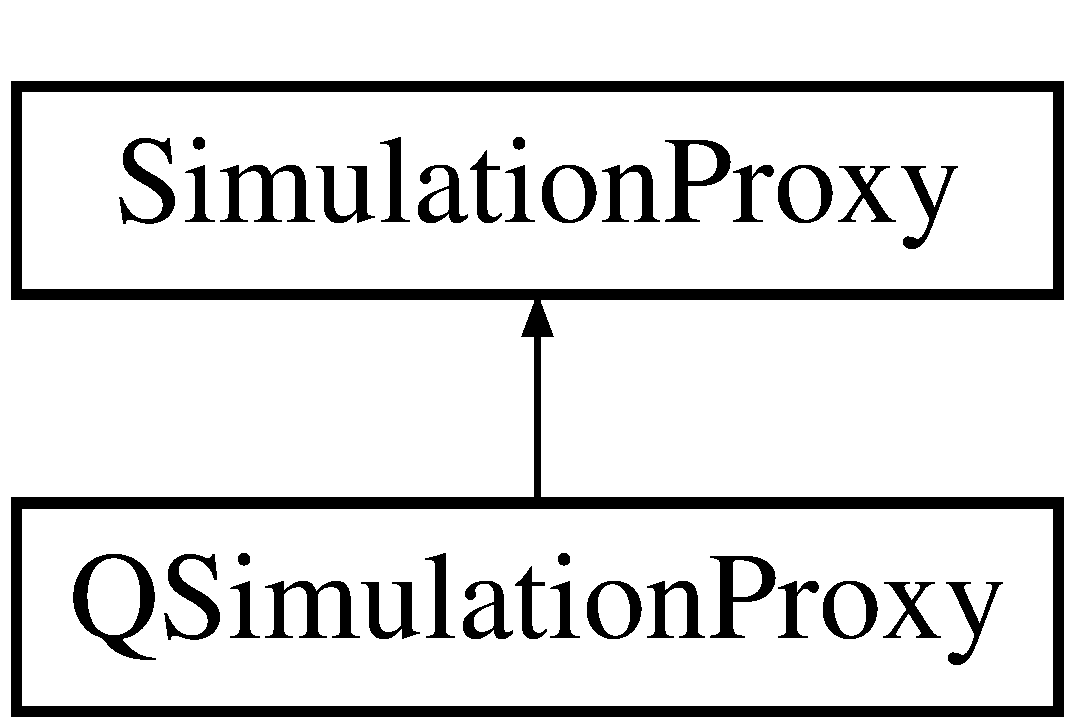
\includegraphics[height=2.000000cm]{class_simulation_proxy}
\end{center}
\end{figure}
\subsection*{Public Types}
\begin{DoxyCompactItemize}
\item 
\mbox{\Hypertarget{class_simulation_proxy_ab558a4c6e83bfa9c30a7f2829aff1c15}\label{class_simulation_proxy_ab558a4c6e83bfa9c30a7f2829aff1c15}} 
enum {\bfseries Status} \{ {\bfseries Not\+Running}, 
{\bfseries Running}, 
{\bfseries Finished}, 
{\bfseries Error}
 \}
\end{DoxyCompactItemize}
\subsection*{Public Member Functions}
\begin{DoxyCompactItemize}
\item 
\mbox{\Hypertarget{class_simulation_proxy_ac1c344b77014b45b858ca19f23097232}\label{class_simulation_proxy_ac1c344b77014b45b858ca19f23097232}} 
virtual void {\bfseries add\+Command} (std\+::string command)=0
\item 
\mbox{\Hypertarget{class_simulation_proxy_adad562cf8271abe74d7f18cede1a9866}\label{class_simulation_proxy_adad562cf8271abe74d7f18cede1a9866}} 
virtual void {\bfseries run} ()=0
\item 
\mbox{\Hypertarget{class_simulation_proxy_a40796f0d728183c412c045918add458b}\label{class_simulation_proxy_a40796f0d728183c412c045918add458b}} 
virtual void {\bfseries terminate} ()=0
\item 
\mbox{\Hypertarget{class_simulation_proxy_aadbe7ca771bd5390e34600f5ddd939bd}\label{class_simulation_proxy_aadbe7ca771bd5390e34600f5ddd939bd}} 
virtual Status {\bfseries poll\+Status} ()=0
\item 
\mbox{\Hypertarget{class_simulation_proxy_a5155fa6c65e9484c3b8d1f6da08cc2c2}\label{class_simulation_proxy_a5155fa6c65e9484c3b8d1f6da08cc2c2}} 
virtual std\+::string const {\bfseries get\+Program\+Output} ()=0
\item 
\mbox{\Hypertarget{class_simulation_proxy_ae9e11cbf59c4b41f9c495756d2d174a9}\label{class_simulation_proxy_ae9e11cbf59c4b41f9c495756d2d174a9}} 
virtual std\+::string const {\bfseries get\+Exe\+Path} ()=0
\end{DoxyCompactItemize}


\subsection{Detailed Description}
IO stream interface abstraction. 

Interface class for future use in different environments 

The documentation for this class was generated from the following file\+:\begin{DoxyCompactItemize}
\item 
xfoil/\hyperlink{simulation__proxy_8h}{simulation\+\_\+proxy.\+h}\end{DoxyCompactItemize}

\hypertarget{class_simulation_scheduler}{}\section{Simulation\+Scheduler Class Reference}
\label{class_simulation_scheduler}\index{Simulation\+Scheduler@{Simulation\+Scheduler}}


Class controlling execution of external simulation tools.  




{\ttfamily \#include $<$simulation.\+h$>$}

Inheritance diagram for Simulation\+Scheduler\+:\begin{figure}[H]
\begin{center}
\leavevmode
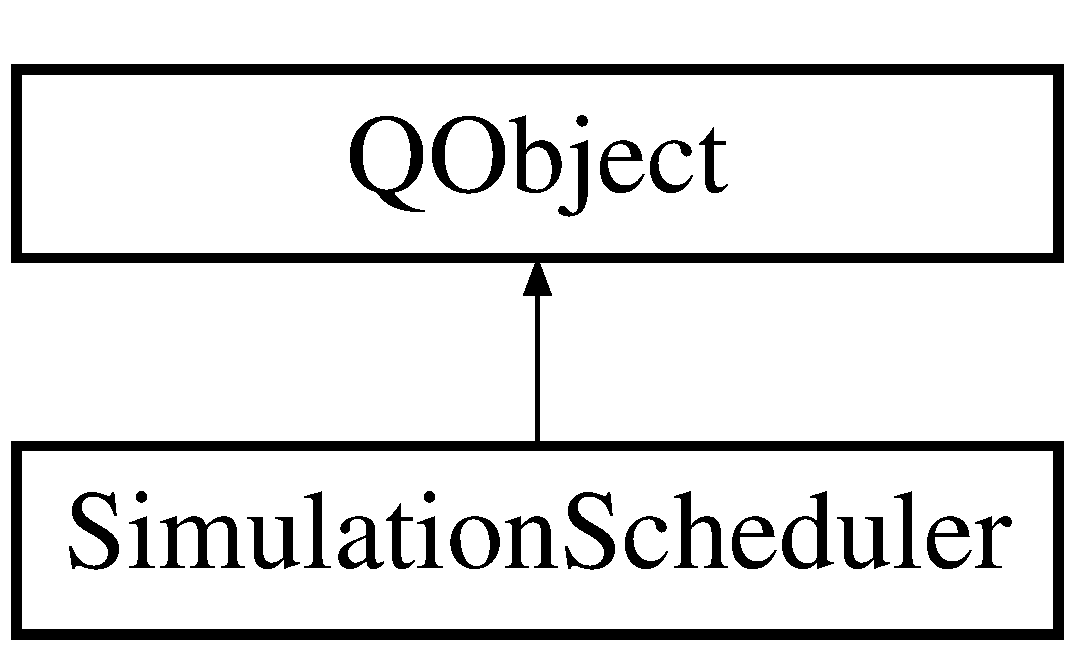
\includegraphics[height=2.000000cm]{class_simulation_scheduler}
\end{center}
\end{figure}
\subsection*{Public Slots}
\begin{DoxyCompactItemize}
\item 
\hypertarget{class_simulation_scheduler_ae48b5f2f68304c077d890c4dbe882e4f}{}\label{class_simulation_scheduler_ae48b5f2f68304c077d890c4dbe882e4f} 
void {\bfseries update\+State} (bool state)
\item 
\hypertarget{class_simulation_scheduler_a060a51e44f3f6e51b1631fc3a41194d0}{}\label{class_simulation_scheduler_a060a51e44f3f6e51b1631fc3a41194d0} 
void {\bfseries worker\+Finished} ()
\item 
\hypertarget{class_simulation_scheduler_a27ad04f596b98dcf32e02fe0104a062b}{}\label{class_simulation_scheduler_a27ad04f596b98dcf32e02fe0104a062b} 
void {\bfseries error\+String} (Q\+String str)
\end{DoxyCompactItemize}
\subsection*{Signals}
\begin{DoxyCompactItemize}
\item 
\hypertarget{class_simulation_scheduler_a0984b261f42cb46e75c4042349922e19}{}\label{class_simulation_scheduler_a0984b261f42cb46e75c4042349922e19} 
void {\bfseries stop\+Worker} ()
\item 
\hypertarget{class_simulation_scheduler_a1b99e3a87e300443f93c9e5a37f81530}{}\label{class_simulation_scheduler_a1b99e3a87e300443f93c9e5a37f81530} 
void {\bfseries simulation\+Finished} ()
\end{DoxyCompactItemize}
\subsection*{Public Member Functions}
\begin{DoxyCompactItemize}
\item 
\hypertarget{class_simulation_scheduler_aa0e08acf06360d47589272e592d031b7}{}\label{class_simulation_scheduler_aa0e08acf06360d47589272e592d031b7} 
{\bfseries Simulation\+Scheduler} (\hyperlink{struct_config_1_1_simulation_params}{Config\+::\+Simulation\+Params} params, Q\+Object $\ast$parent=0)
\item 
\hypertarget{class_simulation_scheduler_a2090cc903dea412d1c49dbc6c2bac8c5}{}\label{class_simulation_scheduler_a2090cc903dea412d1c49dbc6c2bac8c5} 
void {\bfseries Add\+Task} (\hyperlink{struct_task}{Task} task)
\item 
\hypertarget{class_simulation_scheduler_afb3ac15bf8920c5cf02da1987c48736a}{}\label{class_simulation_scheduler_afb3ac15bf8920c5cf02da1987c48736a} 
void {\bfseries Add\+Batch\+Task} (std\+::vector$<$ \hyperlink{struct_task}{Task} $>$ \&input)
\item 
\hypertarget{class_simulation_scheduler_aa8bbd350d4174bf069f5466abc33db6e}{}\label{class_simulation_scheduler_aa8bbd350d4174bf069f5466abc33db6e} 
void {\bfseries Wait\+For\+Finished} ()
\item 
\hypertarget{class_simulation_scheduler_a21b6811560eafda46f85ffdee02bcbb2}{}\label{class_simulation_scheduler_a21b6811560eafda46f85ffdee02bcbb2} 
bool {\bfseries Is\+Tasks\+Finished} () const
\end{DoxyCompactItemize}


\subsection{Detailed Description}
Class controlling execution of external simulation tools. 

Controls multiple instances of xfoil optimizer running in parallel Runs a thread that polls and initiates all xfoil proxy instances Has an internal queue for requests 

The documentation for this class was generated from the following file\+:\begin{DoxyCompactItemize}
\item 
xfoil/\hyperlink{simulation_8h}{simulation.\+h}\end{DoxyCompactItemize}

\hypertarget{struct_task}{}\section{Task Struct Reference}
\label{struct_task}\index{Task@{Task}}
\subsection*{Public Member Functions}
\begin{DoxyCompactItemize}
\item 
\hypertarget{struct_task_a065fcc943559671cefeb383652bc30fd}{}\label{struct_task_a065fcc943559671cefeb383652bc30fd} 
{\bfseries Task} (\hyperlink{class_geometry}{Geometry} $\ast$geom)
\end{DoxyCompactItemize}
\subsection*{Public Attributes}
\begin{DoxyCompactItemize}
\item 
\hypertarget{struct_task_a76af73b7a72c92cfc7ca31c88783f7df}{}\label{struct_task_a76af73b7a72c92cfc7ca31c88783f7df} 
\hyperlink{class_geometry}{Geometry} $\ast$ {\bfseries geometry}
\item 
\hypertarget{struct_task_a087808befc05fe735e07b51e2cb5eedf}{}\label{struct_task_a087808befc05fe735e07b51e2cb5eedf} 
int {\bfseries handler\+Assigned} = -\/1
\end{DoxyCompactItemize}


The documentation for this struct was generated from the following file\+:\begin{DoxyCompactItemize}
\item 
xfoil/\hyperlink{simulation_8h}{simulation.\+h}\end{DoxyCompactItemize}

\hypertarget{class_time_manager}{}\section{Time\+Manager Class Reference}
\label{class_time_manager}\index{Time\+Manager@{Time\+Manager}}


Class containing methods to measure time.  




{\ttfamily \#include $<$time\+\_\+manager.\+h$>$}

\subsection*{Static Public Member Functions}
\begin{DoxyCompactItemize}
\item 
\hypertarget{class_time_manager_ad42a2f423c6c3310112abc3c5c742c9e}{}\label{class_time_manager_ad42a2f423c6c3310112abc3c5c742c9e} 
static int {\bfseries get\+Time\+Since\+Start} ()
\item 
\hypertarget{class_time_manager_aff5359efb14111764aa373367bafa9cc}{}\label{class_time_manager_aff5359efb14111764aa373367bafa9cc} 
static std\+::string {\bfseries get\+String\+Time\+Since\+Start} ()
\item 
\hypertarget{class_time_manager_a61b14a72a2f2de8405c8b6b8037561ac}{}\label{class_time_manager_a61b14a72a2f2de8405c8b6b8037561ac} 
static std\+::string {\bfseries get\+String\+Time} ()
\item 
\hypertarget{class_time_manager_ac67de828c7e298b8796c027cafde7479}{}\label{class_time_manager_ac67de828c7e298b8796c027cafde7479} 
static std\+::string {\bfseries get\+String\+Date} ()
\item 
\hypertarget{class_time_manager_a9811ffb8e35957521d0de842ca806206}{}\label{class_time_manager_a9811ffb8e35957521d0de842ca806206} 
static std\+::string {\bfseries get\+String\+Date\+Time} ()
\item 
\hypertarget{class_time_manager_ac9d0eb40ce9e29901f23d5b7b22712ff}{}\label{class_time_manager_ac9d0eb40ce9e29901f23d5b7b22712ff} 
static std\+::string {\bfseries get\+Boot\+Date\+Time} ()
\end{DoxyCompactItemize}


\subsection{Detailed Description}
Class containing methods to measure time. 

Time manager allows to obtain information about current time and date of working application, time and date since application start in integer and string format. 

The documentation for this class was generated from the following files\+:\begin{DoxyCompactItemize}
\item 
utility/\hyperlink{time__manager_8h}{time\+\_\+manager.\+h}\item 
utility/time\+\_\+manager.\+cpp\end{DoxyCompactItemize}

\hypertarget{class_ti_xml_attribute}{}\section{Ti\+Xml\+Attribute Class Reference}
\label{class_ti_xml_attribute}\index{Ti\+Xml\+Attribute@{Ti\+Xml\+Attribute}}


{\ttfamily \#include $<$tinyxml.\+h$>$}

Inheritance diagram for Ti\+Xml\+Attribute\+:\begin{figure}[H]
\begin{center}
\leavevmode
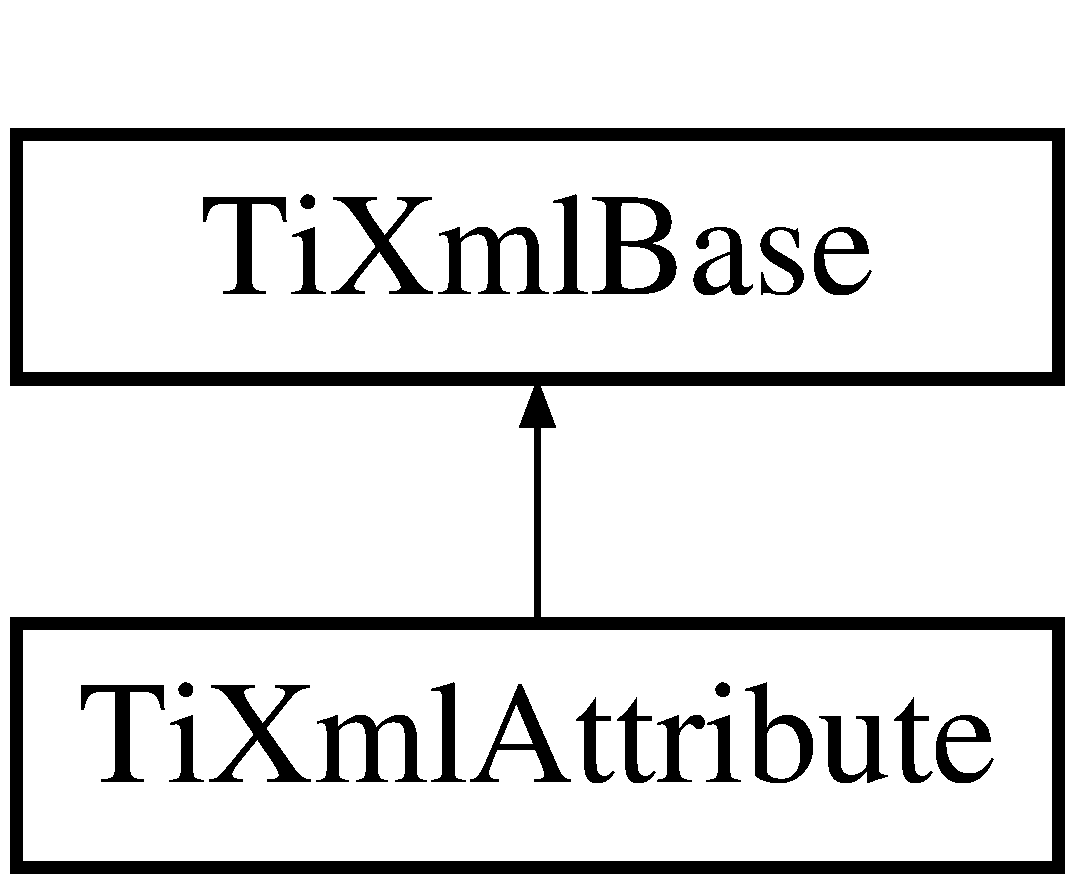
\includegraphics[height=2.000000cm]{class_ti_xml_attribute}
\end{center}
\end{figure}
\subsection*{Public Member Functions}
\begin{DoxyCompactItemize}
\item 
\mbox{\Hypertarget{class_ti_xml_attribute_a9cfa3c8179873fd485d83003b114f8e1}\label{class_ti_xml_attribute_a9cfa3c8179873fd485d83003b114f8e1}} 
\hyperlink{class_ti_xml_attribute_a9cfa3c8179873fd485d83003b114f8e1}{Ti\+Xml\+Attribute} ()
\begin{DoxyCompactList}\small\item\em Construct an empty attribute. \end{DoxyCompactList}\item 
\mbox{\Hypertarget{class_ti_xml_attribute_a052213522caac3979960e0714063861d}\label{class_ti_xml_attribute_a052213522caac3979960e0714063861d}} 
\hyperlink{class_ti_xml_attribute_a052213522caac3979960e0714063861d}{Ti\+Xml\+Attribute} (const std\+::string \&\+\_\+name, const std\+::string \&\+\_\+value)
\begin{DoxyCompactList}\small\item\em std\+::string constructor. \end{DoxyCompactList}\item 
\mbox{\Hypertarget{class_ti_xml_attribute_a759d0b76fb8fcf765ecab243bc14f05e}\label{class_ti_xml_attribute_a759d0b76fb8fcf765ecab243bc14f05e}} 
\hyperlink{class_ti_xml_attribute_a759d0b76fb8fcf765ecab243bc14f05e}{Ti\+Xml\+Attribute} (const char $\ast$\+\_\+name, const char $\ast$\+\_\+value)
\begin{DoxyCompactList}\small\item\em Construct an attribute with a name and value. \end{DoxyCompactList}\item 
\mbox{\Hypertarget{class_ti_xml_attribute_a008ef948268ee752b58c60d63d84bb01}\label{class_ti_xml_attribute_a008ef948268ee752b58c60d63d84bb01}} 
const char $\ast$ \hyperlink{class_ti_xml_attribute_a008ef948268ee752b58c60d63d84bb01}{Name} () const
\begin{DoxyCompactList}\small\item\em Return the name of this attribute. \end{DoxyCompactList}\item 
\mbox{\Hypertarget{class_ti_xml_attribute_ac9f0b56fcacbedb6eb49e5f282bef014}\label{class_ti_xml_attribute_ac9f0b56fcacbedb6eb49e5f282bef014}} 
const char $\ast$ \hyperlink{class_ti_xml_attribute_ac9f0b56fcacbedb6eb49e5f282bef014}{Value} () const
\begin{DoxyCompactList}\small\item\em Return the value of this attribute. \end{DoxyCompactList}\item 
\mbox{\Hypertarget{class_ti_xml_attribute_af70a11c3a0c07e61bd6e215f1f9b24e9}\label{class_ti_xml_attribute_af70a11c3a0c07e61bd6e215f1f9b24e9}} 
const std\+::string \& \hyperlink{class_ti_xml_attribute_af70a11c3a0c07e61bd6e215f1f9b24e9}{Value\+Str} () const
\begin{DoxyCompactList}\small\item\em Return the value of this attribute. \end{DoxyCompactList}\item 
\mbox{\Hypertarget{class_ti_xml_attribute_ac8501370b065df31a35003c81d87cef2}\label{class_ti_xml_attribute_ac8501370b065df31a35003c81d87cef2}} 
int \hyperlink{class_ti_xml_attribute_ac8501370b065df31a35003c81d87cef2}{Int\+Value} () const
\begin{DoxyCompactList}\small\item\em Return the value of this attribute, converted to an integer. \end{DoxyCompactList}\item 
\mbox{\Hypertarget{class_ti_xml_attribute_a8cca240fb2a7130c87b0fc6156e8b34f}\label{class_ti_xml_attribute_a8cca240fb2a7130c87b0fc6156e8b34f}} 
double \hyperlink{class_ti_xml_attribute_a8cca240fb2a7130c87b0fc6156e8b34f}{Double\+Value} () const
\begin{DoxyCompactList}\small\item\em Return the value of this attribute, converted to a double. \end{DoxyCompactList}\item 
\mbox{\Hypertarget{class_ti_xml_attribute_a2bd49ec37463a0a2d081e6587f8b89b8}\label{class_ti_xml_attribute_a2bd49ec37463a0a2d081e6587f8b89b8}} 
const T\+I\+X\+M\+L\+\_\+\+S\+T\+R\+I\+NG \& {\bfseries Name\+T\+Str} () const
\item 
int \hyperlink{class_ti_xml_attribute_a6caa8090d2fbb7966700a16e45ed33de}{Query\+Int\+Value} (int $\ast$\+\_\+value) const
\item 
\mbox{\Hypertarget{class_ti_xml_attribute_a6fa41b710c1b79de37a97004aa600c06}\label{class_ti_xml_attribute_a6fa41b710c1b79de37a97004aa600c06}} 
int \hyperlink{class_ti_xml_attribute_a6fa41b710c1b79de37a97004aa600c06}{Query\+Double\+Value} (double $\ast$\+\_\+value) const
\begin{DoxyCompactList}\small\item\em Query\+Double\+Value examines the value string. See \hyperlink{class_ti_xml_attribute_a6caa8090d2fbb7966700a16e45ed33de}{Query\+Int\+Value()}. \end{DoxyCompactList}\item 
\mbox{\Hypertarget{class_ti_xml_attribute_ab7fa3d21ff8d7c5764cf9af15b667a99}\label{class_ti_xml_attribute_ab7fa3d21ff8d7c5764cf9af15b667a99}} 
void \hyperlink{class_ti_xml_attribute_ab7fa3d21ff8d7c5764cf9af15b667a99}{Set\+Name} (const char $\ast$\+\_\+name)
\begin{DoxyCompactList}\small\item\em Set the name of this attribute. \end{DoxyCompactList}\item 
\mbox{\Hypertarget{class_ti_xml_attribute_a2dae44178f668b3cb48101be4f2236a0}\label{class_ti_xml_attribute_a2dae44178f668b3cb48101be4f2236a0}} 
void \hyperlink{class_ti_xml_attribute_a2dae44178f668b3cb48101be4f2236a0}{Set\+Value} (const char $\ast$\+\_\+value)
\begin{DoxyCompactList}\small\item\em Set the value. \end{DoxyCompactList}\item 
\mbox{\Hypertarget{class_ti_xml_attribute_a7e065df640116a62ea4f4b7da5449cc8}\label{class_ti_xml_attribute_a7e065df640116a62ea4f4b7da5449cc8}} 
void \hyperlink{class_ti_xml_attribute_a7e065df640116a62ea4f4b7da5449cc8}{Set\+Int\+Value} (int \+\_\+value)
\begin{DoxyCompactList}\small\item\em Set the value from an integer. \end{DoxyCompactList}\item 
\mbox{\Hypertarget{class_ti_xml_attribute_a0316da31373496c4368ad549bf711394}\label{class_ti_xml_attribute_a0316da31373496c4368ad549bf711394}} 
void \hyperlink{class_ti_xml_attribute_a0316da31373496c4368ad549bf711394}{Set\+Double\+Value} (double \+\_\+value)
\begin{DoxyCompactList}\small\item\em Set the value from a double. \end{DoxyCompactList}\item 
\mbox{\Hypertarget{class_ti_xml_attribute_ab296ff0c9a8c701055cd257a8a976e57}\label{class_ti_xml_attribute_ab296ff0c9a8c701055cd257a8a976e57}} 
void \hyperlink{class_ti_xml_attribute_ab296ff0c9a8c701055cd257a8a976e57}{Set\+Name} (const std\+::string \&\+\_\+name)
\begin{DoxyCompactList}\small\item\em S\+TL std\+::string form. \end{DoxyCompactList}\item 
\mbox{\Hypertarget{class_ti_xml_attribute_ab43f67a0cc3ec1d80e62606500f0925f}\label{class_ti_xml_attribute_ab43f67a0cc3ec1d80e62606500f0925f}} 
void \hyperlink{class_ti_xml_attribute_ab43f67a0cc3ec1d80e62606500f0925f}{Set\+Value} (const std\+::string \&\+\_\+value)
\begin{DoxyCompactList}\small\item\em S\+TL std\+::string form. \end{DoxyCompactList}\item 
\mbox{\Hypertarget{class_ti_xml_attribute_af2e78f1ba9ed56a26ddc80614ed1c393}\label{class_ti_xml_attribute_af2e78f1ba9ed56a26ddc80614ed1c393}} 
const \hyperlink{class_ti_xml_attribute}{Ti\+Xml\+Attribute} $\ast$ \hyperlink{class_ti_xml_attribute_af2e78f1ba9ed56a26ddc80614ed1c393}{Next} () const
\begin{DoxyCompactList}\small\item\em Get the next sibling attribute in the D\+OM. Returns null at end. \end{DoxyCompactList}\item 
\mbox{\Hypertarget{class_ti_xml_attribute_a138320aa7793b148ba7e5bd0a0ea4db6}\label{class_ti_xml_attribute_a138320aa7793b148ba7e5bd0a0ea4db6}} 
\hyperlink{class_ti_xml_attribute}{Ti\+Xml\+Attribute} $\ast$ {\bfseries Next} ()
\item 
\mbox{\Hypertarget{class_ti_xml_attribute_afc7bbfdf83d59fbc4ff5e283d27b5d7d}\label{class_ti_xml_attribute_afc7bbfdf83d59fbc4ff5e283d27b5d7d}} 
const \hyperlink{class_ti_xml_attribute}{Ti\+Xml\+Attribute} $\ast$ \hyperlink{class_ti_xml_attribute_afc7bbfdf83d59fbc4ff5e283d27b5d7d}{Previous} () const
\begin{DoxyCompactList}\small\item\em Get the previous sibling attribute in the D\+OM. Returns null at beginning. \end{DoxyCompactList}\item 
\mbox{\Hypertarget{class_ti_xml_attribute_ae4dabc932cba945ed1e92fec5f121193}\label{class_ti_xml_attribute_ae4dabc932cba945ed1e92fec5f121193}} 
\hyperlink{class_ti_xml_attribute}{Ti\+Xml\+Attribute} $\ast$ {\bfseries Previous} ()
\item 
\mbox{\Hypertarget{class_ti_xml_attribute_a51eef33c2cdd55831447af46be0baf8b}\label{class_ti_xml_attribute_a51eef33c2cdd55831447af46be0baf8b}} 
bool {\bfseries operator==} (const \hyperlink{class_ti_xml_attribute}{Ti\+Xml\+Attribute} \&rhs) const
\item 
\mbox{\Hypertarget{class_ti_xml_attribute_a80dcb758cc5ab27ce9865301e2da1335}\label{class_ti_xml_attribute_a80dcb758cc5ab27ce9865301e2da1335}} 
bool {\bfseries operator$<$} (const \hyperlink{class_ti_xml_attribute}{Ti\+Xml\+Attribute} \&rhs) const
\item 
\mbox{\Hypertarget{class_ti_xml_attribute_a697c2dde7ac60fccaa7049cee906eb3e}\label{class_ti_xml_attribute_a697c2dde7ac60fccaa7049cee906eb3e}} 
bool {\bfseries operator$>$} (const \hyperlink{class_ti_xml_attribute}{Ti\+Xml\+Attribute} \&rhs) const
\item 
\mbox{\Hypertarget{class_ti_xml_attribute_ad62774421b814894b995af3b5d231dda}\label{class_ti_xml_attribute_ad62774421b814894b995af3b5d231dda}} 
virtual const char $\ast$ {\bfseries Parse} (const char $\ast$p, \hyperlink{class_ti_xml_parsing_data}{Ti\+Xml\+Parsing\+Data} $\ast$data, Ti\+Xml\+Encoding encoding)
\item 
virtual void \hyperlink{class_ti_xml_attribute_a68ae373e03b9c35be4c9d0c3c233b894}{Print} (F\+I\+LE $\ast$cfile, int depth) const
\item 
\mbox{\Hypertarget{class_ti_xml_attribute_a5c8f72a7d1a49972434d45f4c2889e0e}\label{class_ti_xml_attribute_a5c8f72a7d1a49972434d45f4c2889e0e}} 
void {\bfseries Print} (F\+I\+LE $\ast$cfile, int depth, T\+I\+X\+M\+L\+\_\+\+S\+T\+R\+I\+NG $\ast$str) const
\item 
\mbox{\Hypertarget{class_ti_xml_attribute_ac12a94d4548302afb12f488ba101f7d1}\label{class_ti_xml_attribute_ac12a94d4548302afb12f488ba101f7d1}} 
void {\bfseries Set\+Document} (\hyperlink{class_ti_xml_document}{Ti\+Xml\+Document} $\ast$doc)
\end{DoxyCompactItemize}
\subsection*{Friends}
\begin{DoxyCompactItemize}
\item 
\mbox{\Hypertarget{class_ti_xml_attribute_a35a7b7f89f708527677d5078d41ce0bf}\label{class_ti_xml_attribute_a35a7b7f89f708527677d5078d41ce0bf}} 
class {\bfseries Ti\+Xml\+Attribute\+Set}
\end{DoxyCompactItemize}
\subsection*{Additional Inherited Members}


\subsection{Detailed Description}
An attribute is a name-\/value pair. Elements have an arbitrary number of attributes, each with a unique name.

\begin{DoxyNote}{Note}
The attributes are not Ti\+Xml\+Nodes, since they are not part of the tiny\+X\+ML document object model. There are other suggested ways to look at this problem. 
\end{DoxyNote}


\subsection{Member Function Documentation}
\mbox{\Hypertarget{class_ti_xml_attribute_a68ae373e03b9c35be4c9d0c3c233b894}\label{class_ti_xml_attribute_a68ae373e03b9c35be4c9d0c3c233b894}} 
\index{Ti\+Xml\+Attribute@{Ti\+Xml\+Attribute}!Print@{Print}}
\index{Print@{Print}!Ti\+Xml\+Attribute@{Ti\+Xml\+Attribute}}
\subsubsection{\texorpdfstring{Print()}{Print()}}
{\footnotesize\ttfamily virtual void Ti\+Xml\+Attribute\+::\+Print (\begin{DoxyParamCaption}\item[{F\+I\+LE $\ast$}]{cfile,  }\item[{int}]{depth }\end{DoxyParamCaption}) const\hspace{0.3cm}{\ttfamily [inline]}, {\ttfamily [virtual]}}

All Tiny\+Xml classes can print themselves to a filestream or the string class (\hyperlink{class_ti_xml_string}{Ti\+Xml\+String} in non-\/\+S\+TL mode, std\+::string in S\+TL mode.) Either or both cfile and str can be null.

This is a formatted print, and will insert tabs and newlines.

(For an unformatted stream, use the $<$$<$ operator.) 

Implements \hyperlink{class_ti_xml_base_a0de56b3f2ef14c65091a3b916437b512}{Ti\+Xml\+Base}.

\mbox{\Hypertarget{class_ti_xml_attribute_a6caa8090d2fbb7966700a16e45ed33de}\label{class_ti_xml_attribute_a6caa8090d2fbb7966700a16e45ed33de}} 
\index{Ti\+Xml\+Attribute@{Ti\+Xml\+Attribute}!Query\+Int\+Value@{Query\+Int\+Value}}
\index{Query\+Int\+Value@{Query\+Int\+Value}!Ti\+Xml\+Attribute@{Ti\+Xml\+Attribute}}
\subsubsection{\texorpdfstring{Query\+Int\+Value()}{QueryIntValue()}}
{\footnotesize\ttfamily int Ti\+Xml\+Attribute\+::\+Query\+Int\+Value (\begin{DoxyParamCaption}\item[{int $\ast$}]{\+\_\+value }\end{DoxyParamCaption}) const}

Query\+Int\+Value examines the value string. It is an alternative to the \hyperlink{class_ti_xml_attribute_ac8501370b065df31a35003c81d87cef2}{Int\+Value()} method with richer error checking. If the value is an integer, it is stored in \textquotesingle{}value\textquotesingle{} and the call returns T\+I\+X\+M\+L\+\_\+\+S\+U\+C\+C\+E\+SS. If it is not an integer, it returns T\+I\+X\+M\+L\+\_\+\+W\+R\+O\+N\+G\+\_\+\+T\+Y\+PE.

A specialized but useful call. Note that for success it returns 0, which is the opposite of almost all other Tiny\+Xml calls. 

The documentation for this class was generated from the following files\+:\begin{DoxyCompactItemize}
\item 
utility/tiny\+\_\+xml/tinyxml.\+h\item 
utility/tiny\+\_\+xml/tinyxml.\+cpp\item 
utility/tiny\+\_\+xml/tinyxmlparser.\+cpp\end{DoxyCompactItemize}

\hypertarget{class_ti_xml_attribute_set}{}\section{Ti\+Xml\+Attribute\+Set Class Reference}
\label{class_ti_xml_attribute_set}\index{Ti\+Xml\+Attribute\+Set@{Ti\+Xml\+Attribute\+Set}}
\subsection*{Public Member Functions}
\begin{DoxyCompactItemize}
\item 
\mbox{\Hypertarget{class_ti_xml_attribute_set_a745e50ddaae3bee93e4589321e0b9c1a}\label{class_ti_xml_attribute_set_a745e50ddaae3bee93e4589321e0b9c1a}} 
void {\bfseries Add} (\hyperlink{class_ti_xml_attribute}{Ti\+Xml\+Attribute} $\ast$attribute)
\item 
\mbox{\Hypertarget{class_ti_xml_attribute_set_a924a73d071f2573f9060f0be57879c57}\label{class_ti_xml_attribute_set_a924a73d071f2573f9060f0be57879c57}} 
void {\bfseries Remove} (\hyperlink{class_ti_xml_attribute}{Ti\+Xml\+Attribute} $\ast$attribute)
\item 
\mbox{\Hypertarget{class_ti_xml_attribute_set_a85dfd2b5bae45c94334dced146f5c11a}\label{class_ti_xml_attribute_set_a85dfd2b5bae45c94334dced146f5c11a}} 
const \hyperlink{class_ti_xml_attribute}{Ti\+Xml\+Attribute} $\ast$ {\bfseries First} () const
\item 
\mbox{\Hypertarget{class_ti_xml_attribute_set_a99703bb08ca2aece2d7ef835de339ba0}\label{class_ti_xml_attribute_set_a99703bb08ca2aece2d7ef835de339ba0}} 
\hyperlink{class_ti_xml_attribute}{Ti\+Xml\+Attribute} $\ast$ {\bfseries First} ()
\item 
\mbox{\Hypertarget{class_ti_xml_attribute_set_a3b0d49f3802effcf377f32d9a359302c}\label{class_ti_xml_attribute_set_a3b0d49f3802effcf377f32d9a359302c}} 
const \hyperlink{class_ti_xml_attribute}{Ti\+Xml\+Attribute} $\ast$ {\bfseries Last} () const
\item 
\mbox{\Hypertarget{class_ti_xml_attribute_set_ab4c4edfb2d74f6ea31aae096743bd6e0}\label{class_ti_xml_attribute_set_ab4c4edfb2d74f6ea31aae096743bd6e0}} 
\hyperlink{class_ti_xml_attribute}{Ti\+Xml\+Attribute} $\ast$ {\bfseries Last} ()
\item 
\mbox{\Hypertarget{class_ti_xml_attribute_set_a6d4f03bb84f70c78171db27a869225c1}\label{class_ti_xml_attribute_set_a6d4f03bb84f70c78171db27a869225c1}} 
\hyperlink{class_ti_xml_attribute}{Ti\+Xml\+Attribute} $\ast$ {\bfseries Find} (const char $\ast$\+\_\+name) const
\item 
\mbox{\Hypertarget{class_ti_xml_attribute_set_a5e28f5d32f048fba85d04dc317495bdc}\label{class_ti_xml_attribute_set_a5e28f5d32f048fba85d04dc317495bdc}} 
\hyperlink{class_ti_xml_attribute}{Ti\+Xml\+Attribute} $\ast$ {\bfseries Find\+Or\+Create} (const char $\ast$\+\_\+name)
\item 
\mbox{\Hypertarget{class_ti_xml_attribute_set_a828d42fe3db4ed78bba9ab270190c670}\label{class_ti_xml_attribute_set_a828d42fe3db4ed78bba9ab270190c670}} 
\hyperlink{class_ti_xml_attribute}{Ti\+Xml\+Attribute} $\ast$ {\bfseries Find} (const std\+::string \&\+\_\+name) const
\item 
\mbox{\Hypertarget{class_ti_xml_attribute_set_acccd76e3d87a92caed2795266c6e540e}\label{class_ti_xml_attribute_set_acccd76e3d87a92caed2795266c6e540e}} 
\hyperlink{class_ti_xml_attribute}{Ti\+Xml\+Attribute} $\ast$ {\bfseries Find\+Or\+Create} (const std\+::string \&\+\_\+name)
\end{DoxyCompactItemize}


The documentation for this class was generated from the following files\+:\begin{DoxyCompactItemize}
\item 
utility/tiny\+\_\+xml/tinyxml.\+h\item 
utility/tiny\+\_\+xml/tinyxml.\+cpp\end{DoxyCompactItemize}

\hypertarget{class_ti_xml_base}{}\section{Ti\+Xml\+Base Class Reference}
\label{class_ti_xml_base}\index{Ti\+Xml\+Base@{Ti\+Xml\+Base}}


{\ttfamily \#include $<$tinyxml.\+h$>$}

Inheritance diagram for Ti\+Xml\+Base\+:\begin{figure}[H]
\begin{center}
\leavevmode
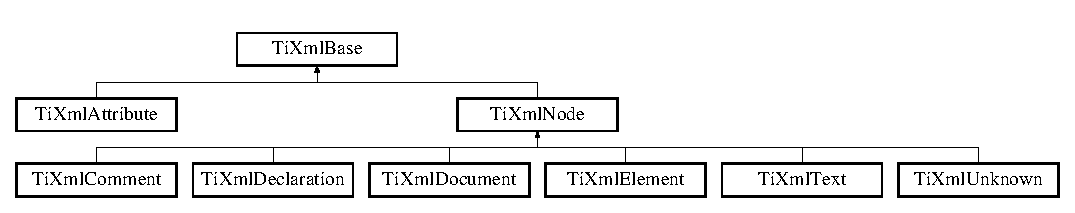
\includegraphics[height=2.413793cm]{class_ti_xml_base}
\end{center}
\end{figure}
\subsection*{Public Types}
\begin{DoxyCompactItemize}
\item 
\hypertarget{class_ti_xml_base_a9a7e9344415956ab96e8c75f6a0bbd48}{}\label{class_ti_xml_base_a9a7e9344415956ab96e8c75f6a0bbd48} 
enum \{ \newline
{\bfseries T\+I\+X\+M\+L\+\_\+\+N\+O\+\_\+\+E\+R\+R\+OR} = 0, 
{\bfseries T\+I\+X\+M\+L\+\_\+\+E\+R\+R\+OR}, 
{\bfseries T\+I\+X\+M\+L\+\_\+\+E\+R\+R\+O\+R\+\_\+\+O\+P\+E\+N\+I\+N\+G\+\_\+\+F\+I\+LE}, 
{\bfseries T\+I\+X\+M\+L\+\_\+\+E\+R\+R\+O\+R\+\_\+\+P\+A\+R\+S\+I\+N\+G\+\_\+\+E\+L\+E\+M\+E\+NT}, 
\newline
{\bfseries T\+I\+X\+M\+L\+\_\+\+E\+R\+R\+O\+R\+\_\+\+F\+A\+I\+L\+E\+D\+\_\+\+T\+O\+\_\+\+R\+E\+A\+D\+\_\+\+E\+L\+E\+M\+E\+N\+T\+\_\+\+N\+A\+ME}, 
{\bfseries T\+I\+X\+M\+L\+\_\+\+E\+R\+R\+O\+R\+\_\+\+R\+E\+A\+D\+I\+N\+G\+\_\+\+E\+L\+E\+M\+E\+N\+T\+\_\+\+V\+A\+L\+UE}, 
{\bfseries T\+I\+X\+M\+L\+\_\+\+E\+R\+R\+O\+R\+\_\+\+R\+E\+A\+D\+I\+N\+G\+\_\+\+A\+T\+T\+R\+I\+B\+U\+T\+ES}, 
{\bfseries T\+I\+X\+M\+L\+\_\+\+E\+R\+R\+O\+R\+\_\+\+P\+A\+R\+S\+I\+N\+G\+\_\+\+E\+M\+P\+TY}, 
\newline
{\bfseries T\+I\+X\+M\+L\+\_\+\+E\+R\+R\+O\+R\+\_\+\+R\+E\+A\+D\+I\+N\+G\+\_\+\+E\+N\+D\+\_\+\+T\+AG}, 
{\bfseries T\+I\+X\+M\+L\+\_\+\+E\+R\+R\+O\+R\+\_\+\+P\+A\+R\+S\+I\+N\+G\+\_\+\+U\+N\+K\+N\+O\+WN}, 
{\bfseries T\+I\+X\+M\+L\+\_\+\+E\+R\+R\+O\+R\+\_\+\+P\+A\+R\+S\+I\+N\+G\+\_\+\+C\+O\+M\+M\+E\+NT}, 
{\bfseries T\+I\+X\+M\+L\+\_\+\+E\+R\+R\+O\+R\+\_\+\+P\+A\+R\+S\+I\+N\+G\+\_\+\+D\+E\+C\+L\+A\+R\+A\+T\+I\+ON}, 
\newline
{\bfseries T\+I\+X\+M\+L\+\_\+\+E\+R\+R\+O\+R\+\_\+\+D\+O\+C\+U\+M\+E\+N\+T\+\_\+\+E\+M\+P\+TY}, 
{\bfseries T\+I\+X\+M\+L\+\_\+\+E\+R\+R\+O\+R\+\_\+\+E\+M\+B\+E\+D\+D\+E\+D\+\_\+\+N\+U\+LL}, 
{\bfseries T\+I\+X\+M\+L\+\_\+\+E\+R\+R\+O\+R\+\_\+\+P\+A\+R\+S\+I\+N\+G\+\_\+\+C\+D\+A\+TA}, 
{\bfseries T\+I\+X\+M\+L\+\_\+\+E\+R\+R\+O\+R\+\_\+\+D\+O\+C\+U\+M\+E\+N\+T\+\_\+\+T\+O\+P\+\_\+\+O\+N\+LY}, 
\newline
{\bfseries T\+I\+X\+M\+L\+\_\+\+E\+R\+R\+O\+R\+\_\+\+S\+T\+R\+I\+N\+G\+\_\+\+C\+O\+U\+NT}
 \}
\end{DoxyCompactItemize}
\subsection*{Public Member Functions}
\begin{DoxyCompactItemize}
\item 
virtual void \hyperlink{class_ti_xml_base_a0de56b3f2ef14c65091a3b916437b512}{Print} (F\+I\+LE $\ast$cfile, int depth) const =0
\item 
int \hyperlink{class_ti_xml_base_ad0cacca5d76d156b26511f46080b442e}{Row} () const
\item 
\hypertarget{class_ti_xml_base_ad283b95d9858d5d78c334f4a61b07bb4}{}\label{class_ti_xml_base_ad283b95d9858d5d78c334f4a61b07bb4} 
int \hyperlink{class_ti_xml_base_ad283b95d9858d5d78c334f4a61b07bb4}{Column} () const
\begin{DoxyCompactList}\small\item\em See \hyperlink{class_ti_xml_base_ad0cacca5d76d156b26511f46080b442e}{Row()} \end{DoxyCompactList}\item 
\hypertarget{class_ti_xml_base_ac6b3e0f790930d4970ec30764e937b5d}{}\label{class_ti_xml_base_ac6b3e0f790930d4970ec30764e937b5d} 
void \hyperlink{class_ti_xml_base_ac6b3e0f790930d4970ec30764e937b5d}{Set\+User\+Data} (void $\ast$user)
\begin{DoxyCompactList}\small\item\em Set a pointer to arbitrary user data. \end{DoxyCompactList}\item 
\hypertarget{class_ti_xml_base_a6559a530ca6763fc301a14d77ed28c17}{}\label{class_ti_xml_base_a6559a530ca6763fc301a14d77ed28c17} 
void $\ast$ \hyperlink{class_ti_xml_base_a6559a530ca6763fc301a14d77ed28c17}{Get\+User\+Data} ()
\begin{DoxyCompactList}\small\item\em Get a pointer to arbitrary user data. \end{DoxyCompactList}\item 
\hypertarget{class_ti_xml_base_aaaaefcef8c0e6e32f8920f4982b2daf3}{}\label{class_ti_xml_base_aaaaefcef8c0e6e32f8920f4982b2daf3} 
const void $\ast$ \hyperlink{class_ti_xml_base_aaaaefcef8c0e6e32f8920f4982b2daf3}{Get\+User\+Data} () const
\begin{DoxyCompactList}\small\item\em Get a pointer to arbitrary user data. \end{DoxyCompactList}\item 
\hypertarget{class_ti_xml_base_a00e4edb0219d00a1379c856e5a1d2025}{}\label{class_ti_xml_base_a00e4edb0219d00a1379c856e5a1d2025} 
virtual const char $\ast$ {\bfseries Parse} (const char $\ast$p, \hyperlink{class_ti_xml_parsing_data}{Ti\+Xml\+Parsing\+Data} $\ast$data, Ti\+Xml\+Encoding encoding)=0
\end{DoxyCompactItemize}
\subsection*{Static Public Member Functions}
\begin{DoxyCompactItemize}
\item 
static void \hyperlink{class_ti_xml_base_a0f799ec645bfb8d8a969e83478f379c1}{Set\+Condense\+White\+Space} (bool condense)
\item 
\hypertarget{class_ti_xml_base_ad4b1472531c647a25b1840a87ae42438}{}\label{class_ti_xml_base_ad4b1472531c647a25b1840a87ae42438} 
static bool \hyperlink{class_ti_xml_base_ad4b1472531c647a25b1840a87ae42438}{Is\+White\+Space\+Condensed} ()
\begin{DoxyCompactList}\small\item\em Return the current white space setting. \end{DoxyCompactList}\item 
static void \hyperlink{class_ti_xml_base_a32ed202562b58de64c7d799ca3c9db98}{Encode\+String} (const T\+I\+X\+M\+L\+\_\+\+S\+T\+R\+I\+NG \&str, T\+I\+X\+M\+L\+\_\+\+S\+T\+R\+I\+NG $\ast$out)
\end{DoxyCompactItemize}
\subsection*{Static Public Attributes}
\begin{DoxyCompactItemize}
\item 
static const int {\bfseries utf8\+Byte\+Table} \mbox{[}256\mbox{]}
\end{DoxyCompactItemize}
\subsection*{Static Protected Member Functions}
\begin{DoxyCompactItemize}
\item 
\hypertarget{class_ti_xml_base_ac0c3d66d8a9e6996a1fa016275e16875}{}\label{class_ti_xml_base_ac0c3d66d8a9e6996a1fa016275e16875} 
static const char $\ast$ {\bfseries Skip\+White\+Space} (const char $\ast$, Ti\+Xml\+Encoding encoding)
\item 
\hypertarget{class_ti_xml_base_af56296d561c0bab4bc8e198cdcf5c48e}{}\label{class_ti_xml_base_af56296d561c0bab4bc8e198cdcf5c48e} 
static bool {\bfseries Is\+White\+Space} (char c)
\item 
\hypertarget{class_ti_xml_base_a3de391ea9f4c4a8aa10d04480b048795}{}\label{class_ti_xml_base_a3de391ea9f4c4a8aa10d04480b048795} 
static bool {\bfseries Is\+White\+Space} (int c)
\item 
\hypertarget{class_ti_xml_base_a189eaa418ff6628bdabf4bf8fb1bd633}{}\label{class_ti_xml_base_a189eaa418ff6628bdabf4bf8fb1bd633} 
static bool {\bfseries Stream\+White\+Space} (std\+::istream $\ast$in, T\+I\+X\+M\+L\+\_\+\+S\+T\+R\+I\+NG $\ast$tag)
\item 
\hypertarget{class_ti_xml_base_aae465f424a9bcf7a9cf2426c62da8e6b}{}\label{class_ti_xml_base_aae465f424a9bcf7a9cf2426c62da8e6b} 
static bool {\bfseries Stream\+To} (std\+::istream $\ast$in, int character, T\+I\+X\+M\+L\+\_\+\+S\+T\+R\+I\+NG $\ast$tag)
\item 
\hypertarget{class_ti_xml_base_a1c21a6ab5f7b503acd91f35f183734b3}{}\label{class_ti_xml_base_a1c21a6ab5f7b503acd91f35f183734b3} 
static const char $\ast$ {\bfseries Read\+Name} (const char $\ast$p, T\+I\+X\+M\+L\+\_\+\+S\+T\+R\+I\+NG $\ast$name, Ti\+Xml\+Encoding encoding)
\item 
\hypertarget{class_ti_xml_base_aa646c74921aa33156968b802bbf5566e}{}\label{class_ti_xml_base_aa646c74921aa33156968b802bbf5566e} 
static const char $\ast$ {\bfseries Read\+Text} (const char $\ast$in, T\+I\+X\+M\+L\+\_\+\+S\+T\+R\+I\+NG $\ast$text, bool ignore\+White\+Space, const char $\ast$end\+Tag, bool ignore\+Case, Ti\+Xml\+Encoding encoding)
\item 
\hypertarget{class_ti_xml_base_ac5c08bf3deffcda0bf8ce2958372b584}{}\label{class_ti_xml_base_ac5c08bf3deffcda0bf8ce2958372b584} 
static const char $\ast$ {\bfseries Get\+Entity} (const char $\ast$in, char $\ast$value, int $\ast$length, Ti\+Xml\+Encoding encoding)
\item 
\hypertarget{class_ti_xml_base_a5b0fde72d6f662ae1fd6303195d2159b}{}\label{class_ti_xml_base_a5b0fde72d6f662ae1fd6303195d2159b} 
static const char $\ast$ {\bfseries Get\+Char} (const char $\ast$p, char $\ast$\+\_\+value, int $\ast$length, Ti\+Xml\+Encoding encoding)
\item 
\hypertarget{class_ti_xml_base_a51631e6986179558b9e5850723ed165a}{}\label{class_ti_xml_base_a51631e6986179558b9e5850723ed165a} 
static bool {\bfseries String\+Equal} (const char $\ast$p, const char $\ast$end\+Tag, bool ignore\+Case, Ti\+Xml\+Encoding encoding)
\item 
\hypertarget{class_ti_xml_base_ae22522b2e8e1ac43102d16394f639fc8}{}\label{class_ti_xml_base_ae22522b2e8e1ac43102d16394f639fc8} 
static int {\bfseries Is\+Alpha} (unsigned char any\+Byte, Ti\+Xml\+Encoding encoding)
\item 
\hypertarget{class_ti_xml_base_a321919055c115c78ded17f85a793f368}{}\label{class_ti_xml_base_a321919055c115c78ded17f85a793f368} 
static int {\bfseries Is\+Alpha\+Num} (unsigned char any\+Byte, Ti\+Xml\+Encoding encoding)
\item 
\hypertarget{class_ti_xml_base_a799f17405a86a5c2029618e85f11a097}{}\label{class_ti_xml_base_a799f17405a86a5c2029618e85f11a097} 
static int {\bfseries To\+Lower} (int v, Ti\+Xml\+Encoding encoding)
\item 
\hypertarget{class_ti_xml_base_a07c765e3a7f979d343e646ea797b180b}{}\label{class_ti_xml_base_a07c765e3a7f979d343e646ea797b180b} 
static void {\bfseries Convert\+U\+T\+F32\+To\+U\+T\+F8} (unsigned long input, char $\ast$output, int $\ast$length)
\end{DoxyCompactItemize}
\subsection*{Protected Attributes}
\begin{DoxyCompactItemize}
\item 
\hypertarget{class_ti_xml_base_a0d992580f3bc264909f898e942677a3c}{}\label{class_ti_xml_base_a0d992580f3bc264909f898e942677a3c} 
\hyperlink{struct_ti_xml_cursor}{Ti\+Xml\+Cursor} {\bfseries location}
\item 
\hypertarget{class_ti_xml_base_ab242c01590191f644569fa89a080d97c}{}\label{class_ti_xml_base_ab242c01590191f644569fa89a080d97c} 
void $\ast$ \hyperlink{class_ti_xml_base_ab242c01590191f644569fa89a080d97c}{user\+Data}
\begin{DoxyCompactList}\small\item\em Field containing a generic user pointer. \end{DoxyCompactList}\end{DoxyCompactItemize}
\subsection*{Static Protected Attributes}
\begin{DoxyCompactItemize}
\item 
static const char $\ast$ {\bfseries error\+String} \mbox{[}T\+I\+X\+M\+L\+\_\+\+E\+R\+R\+O\+R\+\_\+\+S\+T\+R\+I\+N\+G\+\_\+\+C\+O\+U\+NT\mbox{]}
\end{DoxyCompactItemize}
\subsection*{Friends}
\begin{DoxyCompactItemize}
\item 
\hypertarget{class_ti_xml_base_a218872a0d985ae30e78c55adc4bdb196}{}\label{class_ti_xml_base_a218872a0d985ae30e78c55adc4bdb196} 
class {\bfseries Ti\+Xml\+Node}
\item 
\hypertarget{class_ti_xml_base_ab6592e32cb9132be517cc12a70564c4b}{}\label{class_ti_xml_base_ab6592e32cb9132be517cc12a70564c4b} 
class {\bfseries Ti\+Xml\+Element}
\item 
\hypertarget{class_ti_xml_base_a173617f6dfe902cf484ce5552b950475}{}\label{class_ti_xml_base_a173617f6dfe902cf484ce5552b950475} 
class {\bfseries Ti\+Xml\+Document}
\end{DoxyCompactItemize}


\subsection{Detailed Description}
\hyperlink{class_ti_xml_base}{Ti\+Xml\+Base} is a base class for every class in Tiny\+Xml. It does little except to establish that Tiny\+Xml classes can be printed and provide some utility functions.

In X\+ML, the document and elements can contain other elements and other types of nodes.

\begin{DoxyVerb}A Document can contain: Element (container or leaf)
                        Comment (leaf)
                        Unknown (leaf)
                        Declaration( leaf )

An Element can contain: Element (container or leaf)
                        Text    (leaf)
                        Attributes (not on tree)
                        Comment (leaf)
                        Unknown (leaf)

A Decleration contains: Attributes (not on tree)
\end{DoxyVerb}
 

\subsection{Member Function Documentation}
\hypertarget{class_ti_xml_base_a32ed202562b58de64c7d799ca3c9db98}{}\label{class_ti_xml_base_a32ed202562b58de64c7d799ca3c9db98} 
\index{Ti\+Xml\+Base@{Ti\+Xml\+Base}!Encode\+String@{Encode\+String}}
\index{Encode\+String@{Encode\+String}!Ti\+Xml\+Base@{Ti\+Xml\+Base}}
\subsubsection{\texorpdfstring{Encode\+String()}{EncodeString()}}
{\footnotesize\ttfamily void Ti\+Xml\+Base\+::\+Encode\+String (\begin{DoxyParamCaption}\item[{const T\+I\+X\+M\+L\+\_\+\+S\+T\+R\+I\+NG \&}]{str,  }\item[{T\+I\+X\+M\+L\+\_\+\+S\+T\+R\+I\+NG $\ast$}]{out }\end{DoxyParamCaption})\hspace{0.3cm}{\ttfamily [static]}}

Expands entities in a string. Note this should not contian the tag\textquotesingle{}s \textquotesingle{}$<$\textquotesingle{}, \textquotesingle{}$>$\textquotesingle{}, etc, or they will be transformed into entities! \hypertarget{class_ti_xml_base_a0de56b3f2ef14c65091a3b916437b512}{}\label{class_ti_xml_base_a0de56b3f2ef14c65091a3b916437b512} 
\index{Ti\+Xml\+Base@{Ti\+Xml\+Base}!Print@{Print}}
\index{Print@{Print}!Ti\+Xml\+Base@{Ti\+Xml\+Base}}
\subsubsection{\texorpdfstring{Print()}{Print()}}
{\footnotesize\ttfamily virtual void Ti\+Xml\+Base\+::\+Print (\begin{DoxyParamCaption}\item[{F\+I\+LE $\ast$}]{cfile,  }\item[{int}]{depth }\end{DoxyParamCaption}) const\hspace{0.3cm}{\ttfamily [pure virtual]}}

All Tiny\+Xml classes can print themselves to a filestream or the string class (\hyperlink{class_ti_xml_string}{Ti\+Xml\+String} in non-\/\+S\+TL mode, std\+::string in S\+TL mode.) Either or both cfile and str can be null.

This is a formatted print, and will insert tabs and newlines.

(For an unformatted stream, use the $<$$<$ operator.) 

Implemented in \hyperlink{class_ti_xml_document_aa9e166fae51da603641380a964f21eeb}{Ti\+Xml\+Document}, \hyperlink{class_ti_xml_unknown_a5793fbc48ab3419783c0e866ca2d334e}{Ti\+Xml\+Unknown}, \hyperlink{class_ti_xml_declaration_ae46cff6565f299210ab945e78bf28514}{Ti\+Xml\+Declaration}, \hyperlink{class_ti_xml_text_a75f6895906333894e2574cc8cf77ea79}{Ti\+Xml\+Text}, \hyperlink{class_ti_xml_comment_a873171beac19d40f0eaae945711c98ed}{Ti\+Xml\+Comment}, \hyperlink{class_ti_xml_element_aa31a15cddfb8601a31236fe7d2569fb4}{Ti\+Xml\+Element}, and \hyperlink{class_ti_xml_attribute_a68ae373e03b9c35be4c9d0c3c233b894}{Ti\+Xml\+Attribute}.

\hypertarget{class_ti_xml_base_ad0cacca5d76d156b26511f46080b442e}{}\label{class_ti_xml_base_ad0cacca5d76d156b26511f46080b442e} 
\index{Ti\+Xml\+Base@{Ti\+Xml\+Base}!Row@{Row}}
\index{Row@{Row}!Ti\+Xml\+Base@{Ti\+Xml\+Base}}
\subsubsection{\texorpdfstring{Row()}{Row()}}
{\footnotesize\ttfamily int Ti\+Xml\+Base\+::\+Row (\begin{DoxyParamCaption}{ }\end{DoxyParamCaption}) const\hspace{0.3cm}{\ttfamily [inline]}}

Return the position, in the original source file, of this node or attribute. The row and column are 1-\/based. (That is the first row and first column is 1,1). If the returns values are 0 or less, then the parser does not have a row and column value.

Generally, the row and column value will be set when the Ti\+Xml\+Document\+::\+Load(), \hyperlink{class_ti_xml_document_a4c852a889c02cf251117fd1d9fe1845f}{Ti\+Xml\+Document\+::\+Load\+File()}, or any Ti\+Xml\+Node\+::\+Parse() is called. It will N\+OT be set when the D\+OM was created from operator$>$$>$.

The values reflect the initial load. Once the D\+OM is modified programmatically (by adding or changing nodes and attributes) the new values will N\+OT update to reflect changes in the document.

There is a minor performance cost to computing the row and column. Computation can be disabled if \hyperlink{class_ti_xml_document_a51dac56316f89b35bdb7d0d433ba988e}{Ti\+Xml\+Document\+::\+Set\+Tab\+Size()} is called with 0 as the value.

\begin{DoxySeeAlso}{See also}
\hyperlink{class_ti_xml_document_a51dac56316f89b35bdb7d0d433ba988e}{Ti\+Xml\+Document\+::\+Set\+Tab\+Size()} 
\end{DoxySeeAlso}
\hypertarget{class_ti_xml_base_a0f799ec645bfb8d8a969e83478f379c1}{}\label{class_ti_xml_base_a0f799ec645bfb8d8a969e83478f379c1} 
\index{Ti\+Xml\+Base@{Ti\+Xml\+Base}!Set\+Condense\+White\+Space@{Set\+Condense\+White\+Space}}
\index{Set\+Condense\+White\+Space@{Set\+Condense\+White\+Space}!Ti\+Xml\+Base@{Ti\+Xml\+Base}}
\subsubsection{\texorpdfstring{Set\+Condense\+White\+Space()}{SetCondenseWhiteSpace()}}
{\footnotesize\ttfamily static void Ti\+Xml\+Base\+::\+Set\+Condense\+White\+Space (\begin{DoxyParamCaption}\item[{bool}]{condense }\end{DoxyParamCaption})\hspace{0.3cm}{\ttfamily [inline]}, {\ttfamily [static]}}

The world does not agree on whether white space should be kept or not. In order to make everyone happy, these global, static functions are provided to set whether or not Tiny\+Xml will condense all white space into a single space or not. The default is to condense. Note changing this value is not thread safe. 

\subsection{Member Data Documentation}
\hypertarget{class_ti_xml_base_a7ac8feec4100e446b3d78e1ac0659700}{}\label{class_ti_xml_base_a7ac8feec4100e446b3d78e1ac0659700} 
\index{Ti\+Xml\+Base@{Ti\+Xml\+Base}!error\+String@{error\+String}}
\index{error\+String@{error\+String}!Ti\+Xml\+Base@{Ti\+Xml\+Base}}
\subsubsection{\texorpdfstring{error\+String}{errorString}}
{\footnotesize\ttfamily const char $\ast$ Ti\+Xml\+Base\+::error\+String\hspace{0.3cm}{\ttfamily [static]}, {\ttfamily [protected]}}

{\bfseries Initial value\+:}
\begin{DoxyCode}
=
\{
    \textcolor{stringliteral}{"No error"},
    \textcolor{stringliteral}{"Error"},
    \textcolor{stringliteral}{"Failed to open file"},
    \textcolor{stringliteral}{"Error parsing Element."},
    \textcolor{stringliteral}{"Failed to read Element name"},
    \textcolor{stringliteral}{"Error reading Element value."},
    \textcolor{stringliteral}{"Error reading Attributes."},
    \textcolor{stringliteral}{"Error: empty tag."},
    \textcolor{stringliteral}{"Error reading end tag."},
    \textcolor{stringliteral}{"Error parsing Unknown."},
    \textcolor{stringliteral}{"Error parsing Comment."},
    \textcolor{stringliteral}{"Error parsing Declaration."},
    \textcolor{stringliteral}{"Error document empty."},
    \textcolor{stringliteral}{"Error null (0) or unexpected EOF found in input stream."},
    \textcolor{stringliteral}{"Error parsing CDATA."},
    \textcolor{stringliteral}{"Error when TiXmlDocument added to document, because TiXmlDocument can only be at the root."},
\}
\end{DoxyCode}
\hypertarget{class_ti_xml_base_ac8c86058137bdb4b413c3eca58f2d467}{}\label{class_ti_xml_base_ac8c86058137bdb4b413c3eca58f2d467} 
\index{Ti\+Xml\+Base@{Ti\+Xml\+Base}!utf8\+Byte\+Table@{utf8\+Byte\+Table}}
\index{utf8\+Byte\+Table@{utf8\+Byte\+Table}!Ti\+Xml\+Base@{Ti\+Xml\+Base}}
\subsubsection{\texorpdfstring{utf8\+Byte\+Table}{utf8ByteTable}}
{\footnotesize\ttfamily const int Ti\+Xml\+Base\+::utf8\+Byte\+Table\hspace{0.3cm}{\ttfamily [static]}}

{\bfseries Initial value\+:}
\begin{DoxyCode}
= 
\{
    
        1,  1,  1,  1,  1,  1,  1,  1,  1,  1,  1,  1,  1,  1,  1,  1,  
        1,  1,  1,  1,  1,  1,  1,  1,  1,  1,  1,  1,  1,  1,  1,  1,  
        1,  1,  1,  1,  1,  1,  1,  1,  1,  1,  1,  1,  1,  1,  1,  1,  
        1,  1,  1,  1,  1,  1,  1,  1,  1,  1,  1,  1,  1,  1,  1,  1,  
        1,  1,  1,  1,  1,  1,  1,  1,  1,  1,  1,  1,  1,  1,  1,  1,  
        1,  1,  1,  1,  1,  1,  1,  1,  1,  1,  1,  1,  1,  1,  1,  1,  
        1,  1,  1,  1,  1,  1,  1,  1,  1,  1,  1,  1,  1,  1,  1,  1,  
        1,  1,  1,  1,  1,  1,  1,  1,  1,  1,  1,  1,  1,  1,  1,  1,  
        1,  1,  1,  1,  1,  1,  1,  1,  1,  1,  1,  1,  1,  1,  1,  1,  
        1,  1,  1,  1,  1,  1,  1,  1,  1,  1,  1,  1,  1,  1,  1,  1,  
        1,  1,  1,  1,  1,  1,  1,  1,  1,  1,  1,  1,  1,  1,  1,  1,  
        1,  1,  1,  1,  1,  1,  1,  1,  1,  1,  1,  1,  1,  1,  1,  1,  
        1,  1,  2,  2,  2,  2,  2,  2,  2,  2,  2,  2,  2,  2,  2,  2,  
        2,  2,  2,  2,  2,  2,  2,  2,  2,  2,  2,  2,  2,  2,  2,  2,  
        3,  3,  3,  3,  3,  3,  3,  3,  3,  3,  3,  3,  3,  3,  3,  3,  
        4,  4,  4,  4,  4,  1,  1,  1,  1,  1,  1,  1,  1,  1,  1,  1   
\}
\end{DoxyCode}


The documentation for this class was generated from the following files\+:\begin{DoxyCompactItemize}
\item 
utility/tiny\+\_\+xml/tinyxml.\+h\item 
utility/tiny\+\_\+xml/tinyxml.\+cpp\item 
utility/tiny\+\_\+xml/tinyxmlerror.\+cpp\item 
utility/tiny\+\_\+xml/tinyxmlparser.\+cpp\end{DoxyCompactItemize}

\hypertarget{class_ti_xml_comment}{}\section{Ti\+Xml\+Comment Class Reference}
\label{class_ti_xml_comment}\index{Ti\+Xml\+Comment@{Ti\+Xml\+Comment}}


{\ttfamily \#include $<$tinyxml.\+h$>$}

Inheritance diagram for Ti\+Xml\+Comment\+:\begin{figure}[H]
\begin{center}
\leavevmode
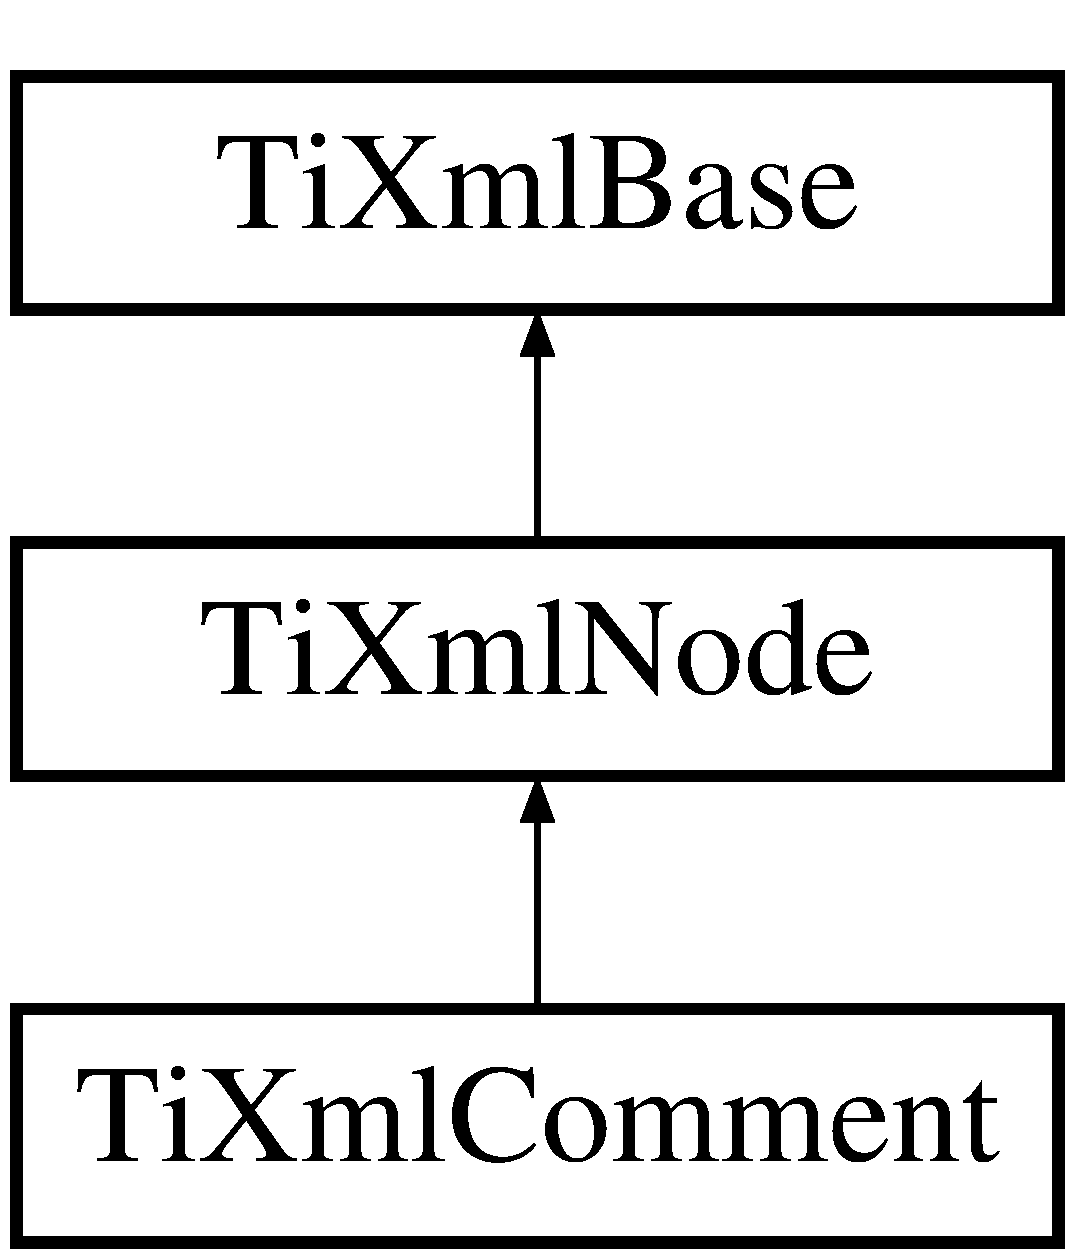
\includegraphics[height=3.000000cm]{class_ti_xml_comment}
\end{center}
\end{figure}
\subsection*{Public Member Functions}
\begin{DoxyCompactItemize}
\item 
\hypertarget{class_ti_xml_comment_aaa3252031d3e8bd3a2bf51a1c61201b7}{}\label{class_ti_xml_comment_aaa3252031d3e8bd3a2bf51a1c61201b7} 
\hyperlink{class_ti_xml_comment_aaa3252031d3e8bd3a2bf51a1c61201b7}{Ti\+Xml\+Comment} ()
\begin{DoxyCompactList}\small\item\em Constructs an empty comment. \end{DoxyCompactList}\item 
\hypertarget{class_ti_xml_comment_a37e7802ef17bc03ebe5ae79bf0713d47}{}\label{class_ti_xml_comment_a37e7802ef17bc03ebe5ae79bf0713d47} 
\hyperlink{class_ti_xml_comment_a37e7802ef17bc03ebe5ae79bf0713d47}{Ti\+Xml\+Comment} (const char $\ast$\+\_\+value)
\begin{DoxyCompactList}\small\item\em Construct a comment from text. \end{DoxyCompactList}\item 
\hypertarget{class_ti_xml_comment_afaec41ac2760ce946ba1590eb5708e50}{}\label{class_ti_xml_comment_afaec41ac2760ce946ba1590eb5708e50} 
{\bfseries Ti\+Xml\+Comment} (const \hyperlink{class_ti_xml_comment}{Ti\+Xml\+Comment} \&)
\item 
\hypertarget{class_ti_xml_comment_aeceedc15f8b8f9ca0b6136696339b3ac}{}\label{class_ti_xml_comment_aeceedc15f8b8f9ca0b6136696339b3ac} 
\hyperlink{class_ti_xml_comment}{Ti\+Xml\+Comment} \& {\bfseries operator=} (const \hyperlink{class_ti_xml_comment}{Ti\+Xml\+Comment} \&base)
\item 
\hypertarget{class_ti_xml_comment_a1f9f06e2ed3f77875093436193b16c16}{}\label{class_ti_xml_comment_a1f9f06e2ed3f77875093436193b16c16} 
virtual \hyperlink{class_ti_xml_node}{Ti\+Xml\+Node} $\ast$ \hyperlink{class_ti_xml_comment_a1f9f06e2ed3f77875093436193b16c16}{Clone} () const
\begin{DoxyCompactList}\small\item\em Returns a copy of this Comment. \end{DoxyCompactList}\item 
virtual void \hyperlink{class_ti_xml_comment_a873171beac19d40f0eaae945711c98ed}{Print} (F\+I\+LE $\ast$cfile, int depth) const
\item 
\hypertarget{class_ti_xml_comment_a43bddc18ac057734b41d84653b71d3e0}{}\label{class_ti_xml_comment_a43bddc18ac057734b41d84653b71d3e0} 
virtual const char $\ast$ {\bfseries Parse} (const char $\ast$p, \hyperlink{class_ti_xml_parsing_data}{Ti\+Xml\+Parsing\+Data} $\ast$data, Ti\+Xml\+Encoding encoding)
\item 
\hypertarget{class_ti_xml_comment_a1032e176d3eb73017ceabc698cac0f16}{}\label{class_ti_xml_comment_a1032e176d3eb73017ceabc698cac0f16} 
virtual const \hyperlink{class_ti_xml_comment}{Ti\+Xml\+Comment} $\ast$ \hyperlink{class_ti_xml_comment_a1032e176d3eb73017ceabc698cac0f16}{To\+Comment} () const
\begin{DoxyCompactList}\small\item\em Cast to a more defined type. Will return null not of the requested type. \end{DoxyCompactList}\item 
\hypertarget{class_ti_xml_comment_acc7c7e07e13c23f17797d642981511df}{}\label{class_ti_xml_comment_acc7c7e07e13c23f17797d642981511df} 
virtual \hyperlink{class_ti_xml_comment}{Ti\+Xml\+Comment} $\ast$ \hyperlink{class_ti_xml_comment_acc7c7e07e13c23f17797d642981511df}{To\+Comment} ()
\begin{DoxyCompactList}\small\item\em Cast to a more defined type. Will return null not of the requested type. \end{DoxyCompactList}\item 
virtual bool \hyperlink{class_ti_xml_comment_ac894241530d1d266131a5026cb251a95}{Accept} (\hyperlink{class_ti_xml_visitor}{Ti\+Xml\+Visitor} $\ast$visitor) const
\end{DoxyCompactItemize}
\subsection*{Protected Member Functions}
\begin{DoxyCompactItemize}
\item 
\hypertarget{class_ti_xml_comment_aaeb8a0b2d503f603879a2d04ceb54295}{}\label{class_ti_xml_comment_aaeb8a0b2d503f603879a2d04ceb54295} 
void {\bfseries Copy\+To} (\hyperlink{class_ti_xml_comment}{Ti\+Xml\+Comment} $\ast$target) const
\item 
\hypertarget{class_ti_xml_comment_a619467ff29c832b101e9b704a23c0357}{}\label{class_ti_xml_comment_a619467ff29c832b101e9b704a23c0357} 
virtual void {\bfseries Stream\+In} (std\+::istream $\ast$in, T\+I\+X\+M\+L\+\_\+\+S\+T\+R\+I\+NG $\ast$tag)
\end{DoxyCompactItemize}
\subsection*{Additional Inherited Members}


\subsection{Detailed Description}
An X\+ML comment. 

\subsection{Member Function Documentation}
\hypertarget{class_ti_xml_comment_ac894241530d1d266131a5026cb251a95}{}\label{class_ti_xml_comment_ac894241530d1d266131a5026cb251a95} 
\index{Ti\+Xml\+Comment@{Ti\+Xml\+Comment}!Accept@{Accept}}
\index{Accept@{Accept}!Ti\+Xml\+Comment@{Ti\+Xml\+Comment}}
\subsubsection{\texorpdfstring{Accept()}{Accept()}}
{\footnotesize\ttfamily bool Ti\+Xml\+Comment\+::\+Accept (\begin{DoxyParamCaption}\item[{\hyperlink{class_ti_xml_visitor}{Ti\+Xml\+Visitor} $\ast$}]{visitor }\end{DoxyParamCaption}) const\hspace{0.3cm}{\ttfamily [virtual]}}

Walk the X\+ML tree visiting this node and all of its children. 

Implements \hyperlink{class_ti_xml_node_acc0f88b7462c6cb73809d410a4f5bb86}{Ti\+Xml\+Node}.

\hypertarget{class_ti_xml_comment_a873171beac19d40f0eaae945711c98ed}{}\label{class_ti_xml_comment_a873171beac19d40f0eaae945711c98ed} 
\index{Ti\+Xml\+Comment@{Ti\+Xml\+Comment}!Print@{Print}}
\index{Print@{Print}!Ti\+Xml\+Comment@{Ti\+Xml\+Comment}}
\subsubsection{\texorpdfstring{Print()}{Print()}}
{\footnotesize\ttfamily void Ti\+Xml\+Comment\+::\+Print (\begin{DoxyParamCaption}\item[{F\+I\+LE $\ast$}]{cfile,  }\item[{int}]{depth }\end{DoxyParamCaption}) const\hspace{0.3cm}{\ttfamily [virtual]}}

All Tiny\+Xml classes can print themselves to a filestream or the string class (\hyperlink{class_ti_xml_string}{Ti\+Xml\+String} in non-\/\+S\+TL mode, std\+::string in S\+TL mode.) Either or both cfile and str can be null.

This is a formatted print, and will insert tabs and newlines.

(For an unformatted stream, use the $<$$<$ operator.) 

Implements \hyperlink{class_ti_xml_base_a0de56b3f2ef14c65091a3b916437b512}{Ti\+Xml\+Base}.



The documentation for this class was generated from the following files\+:\begin{DoxyCompactItemize}
\item 
utility/tiny\+\_\+xml/tinyxml.\+h\item 
utility/tiny\+\_\+xml/tinyxml.\+cpp\item 
utility/tiny\+\_\+xml/tinyxmlparser.\+cpp\end{DoxyCompactItemize}

\hypertarget{struct_ti_xml_cursor}{}\section{Ti\+Xml\+Cursor Struct Reference}
\label{struct_ti_xml_cursor}\index{Ti\+Xml\+Cursor@{Ti\+Xml\+Cursor}}
\subsection*{Public Member Functions}
\begin{DoxyCompactItemize}
\item 
\hypertarget{struct_ti_xml_cursor_a1e6fa622b59dafb71b6efe595105dcdd}{}\label{struct_ti_xml_cursor_a1e6fa622b59dafb71b6efe595105dcdd} 
void {\bfseries Clear} ()
\end{DoxyCompactItemize}
\subsection*{Public Attributes}
\begin{DoxyCompactItemize}
\item 
\hypertarget{struct_ti_xml_cursor_a5b54dd949820c2db061e2be41f3effb3}{}\label{struct_ti_xml_cursor_a5b54dd949820c2db061e2be41f3effb3} 
int {\bfseries row}
\item 
\hypertarget{struct_ti_xml_cursor_a5694d7ed2c4d20109d350c14c417969d}{}\label{struct_ti_xml_cursor_a5694d7ed2c4d20109d350c14c417969d} 
int {\bfseries col}
\end{DoxyCompactItemize}


The documentation for this struct was generated from the following file\+:\begin{DoxyCompactItemize}
\item 
utility/tiny\+\_\+xml/tinyxml.\+h\end{DoxyCompactItemize}

\hypertarget{class_ti_xml_declaration}{}\section{Ti\+Xml\+Declaration Class Reference}
\label{class_ti_xml_declaration}\index{Ti\+Xml\+Declaration@{Ti\+Xml\+Declaration}}


{\ttfamily \#include $<$tinyxml.\+h$>$}

Inheritance diagram for Ti\+Xml\+Declaration\+:\begin{figure}[H]
\begin{center}
\leavevmode
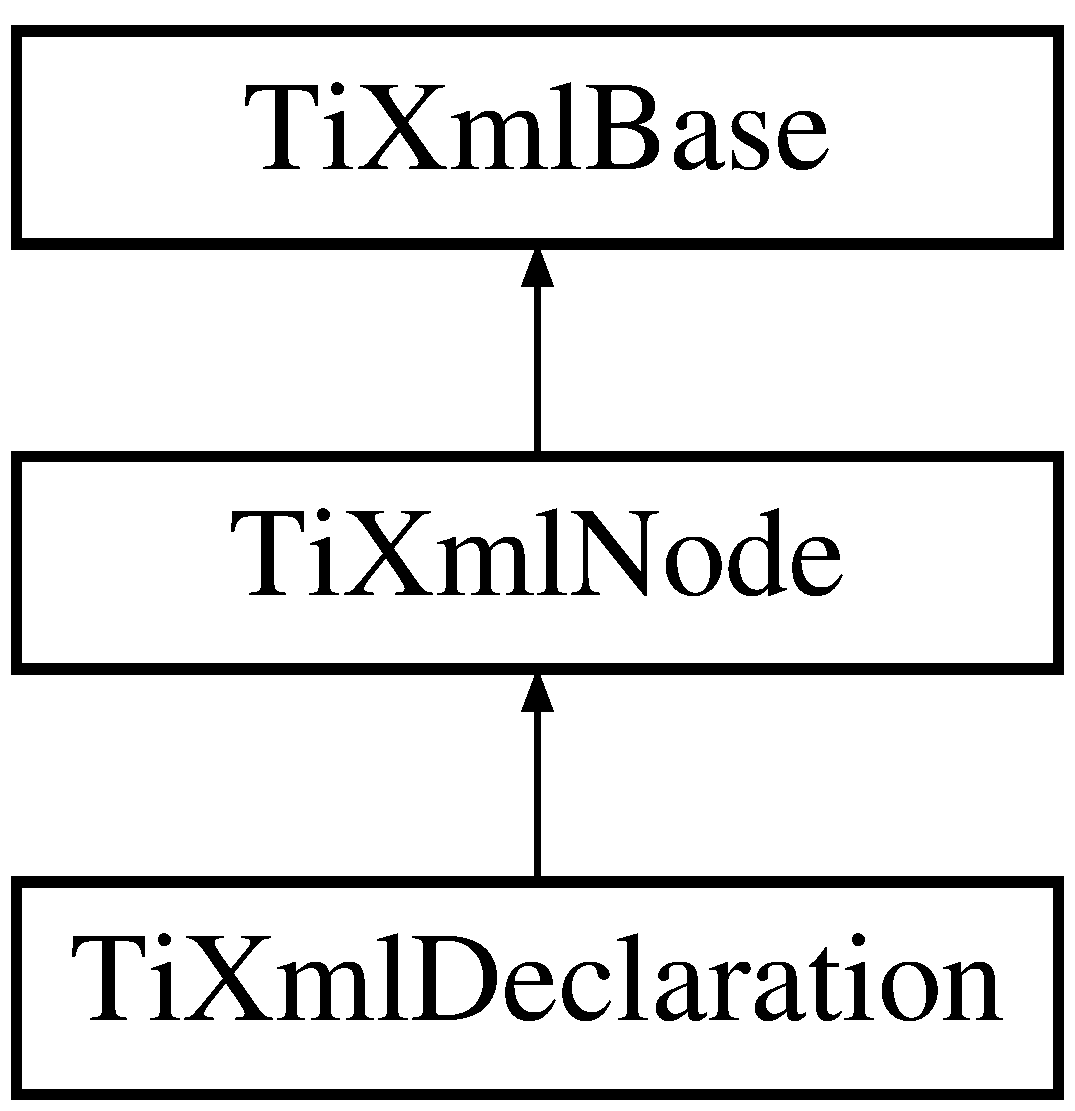
\includegraphics[height=3.000000cm]{class_ti_xml_declaration}
\end{center}
\end{figure}
\subsection*{Public Member Functions}
\begin{DoxyCompactItemize}
\item 
\hypertarget{class_ti_xml_declaration_aa0484d059bea0ea1acb47c9094382d79}{}\label{class_ti_xml_declaration_aa0484d059bea0ea1acb47c9094382d79} 
\hyperlink{class_ti_xml_declaration_aa0484d059bea0ea1acb47c9094382d79}{Ti\+Xml\+Declaration} ()
\begin{DoxyCompactList}\small\item\em Construct an empty declaration. \end{DoxyCompactList}\item 
\hypertarget{class_ti_xml_declaration_acd5556007c3c72209465081de39d9836}{}\label{class_ti_xml_declaration_acd5556007c3c72209465081de39d9836} 
\hyperlink{class_ti_xml_declaration_acd5556007c3c72209465081de39d9836}{Ti\+Xml\+Declaration} (const std\+::string \&\+\_\+version, const std\+::string \&\+\_\+encoding, const std\+::string \&\+\_\+standalone)
\begin{DoxyCompactList}\small\item\em Constructor. \end{DoxyCompactList}\item 
\hypertarget{class_ti_xml_declaration_a3b618d1c30c25e4b7a71f31a595ee298}{}\label{class_ti_xml_declaration_a3b618d1c30c25e4b7a71f31a595ee298} 
\hyperlink{class_ti_xml_declaration_a3b618d1c30c25e4b7a71f31a595ee298}{Ti\+Xml\+Declaration} (const char $\ast$\+\_\+version, const char $\ast$\+\_\+encoding, const char $\ast$\+\_\+standalone)
\begin{DoxyCompactList}\small\item\em Construct. \end{DoxyCompactList}\item 
\hypertarget{class_ti_xml_declaration_a58ac9042c342f7845c8491da0bb091e8}{}\label{class_ti_xml_declaration_a58ac9042c342f7845c8491da0bb091e8} 
{\bfseries Ti\+Xml\+Declaration} (const \hyperlink{class_ti_xml_declaration}{Ti\+Xml\+Declaration} \&copy)
\item 
\hypertarget{class_ti_xml_declaration_a3bc617efe11014ff2b1a9c5727c37a9a}{}\label{class_ti_xml_declaration_a3bc617efe11014ff2b1a9c5727c37a9a} 
\hyperlink{class_ti_xml_declaration}{Ti\+Xml\+Declaration} \& {\bfseries operator=} (const \hyperlink{class_ti_xml_declaration}{Ti\+Xml\+Declaration} \&copy)
\item 
\hypertarget{class_ti_xml_declaration_a95cdcb9354ea220065bd378ffcacc7bd}{}\label{class_ti_xml_declaration_a95cdcb9354ea220065bd378ffcacc7bd} 
const char $\ast$ \hyperlink{class_ti_xml_declaration_a95cdcb9354ea220065bd378ffcacc7bd}{Version} () const
\begin{DoxyCompactList}\small\item\em Version. Will return an empty string if none was found. \end{DoxyCompactList}\item 
\hypertarget{class_ti_xml_declaration_a8d3d1b5b226daa8353276d719497be80}{}\label{class_ti_xml_declaration_a8d3d1b5b226daa8353276d719497be80} 
const char $\ast$ \hyperlink{class_ti_xml_declaration_a8d3d1b5b226daa8353276d719497be80}{Encoding} () const
\begin{DoxyCompactList}\small\item\em Encoding. Will return an empty string if none was found. \end{DoxyCompactList}\item 
\hypertarget{class_ti_xml_declaration_a1f2f8a741593d15a61e491e5024cacef}{}\label{class_ti_xml_declaration_a1f2f8a741593d15a61e491e5024cacef} 
const char $\ast$ \hyperlink{class_ti_xml_declaration_a1f2f8a741593d15a61e491e5024cacef}{Standalone} () const
\begin{DoxyCompactList}\small\item\em Is this a standalone document? \end{DoxyCompactList}\item 
\hypertarget{class_ti_xml_declaration_a35dc1455f69b79e81cae28e186944610}{}\label{class_ti_xml_declaration_a35dc1455f69b79e81cae28e186944610} 
virtual \hyperlink{class_ti_xml_node}{Ti\+Xml\+Node} $\ast$ \hyperlink{class_ti_xml_declaration_a35dc1455f69b79e81cae28e186944610}{Clone} () const
\begin{DoxyCompactList}\small\item\em Creates a copy of this Declaration and returns it. \end{DoxyCompactList}\item 
\hypertarget{class_ti_xml_declaration_ace687d02a5a25a060ae3802abb1b3f55}{}\label{class_ti_xml_declaration_ace687d02a5a25a060ae3802abb1b3f55} 
virtual void {\bfseries Print} (F\+I\+LE $\ast$cfile, int depth, T\+I\+X\+M\+L\+\_\+\+S\+T\+R\+I\+NG $\ast$str) const
\item 
virtual void \hyperlink{class_ti_xml_declaration_ae46cff6565f299210ab945e78bf28514}{Print} (F\+I\+LE $\ast$cfile, int depth) const
\item 
\hypertarget{class_ti_xml_declaration_a9839ea97ed687a2b7342fd7b0f04361b}{}\label{class_ti_xml_declaration_a9839ea97ed687a2b7342fd7b0f04361b} 
virtual const char $\ast$ {\bfseries Parse} (const char $\ast$p, \hyperlink{class_ti_xml_parsing_data}{Ti\+Xml\+Parsing\+Data} $\ast$data, Ti\+Xml\+Encoding encoding)
\item 
\hypertarget{class_ti_xml_declaration_aab62703b620d9b9391b482dc1835ecf6}{}\label{class_ti_xml_declaration_aab62703b620d9b9391b482dc1835ecf6} 
virtual const \hyperlink{class_ti_xml_declaration}{Ti\+Xml\+Declaration} $\ast$ \hyperlink{class_ti_xml_declaration_aab62703b620d9b9391b482dc1835ecf6}{To\+Declaration} () const
\begin{DoxyCompactList}\small\item\em Cast to a more defined type. Will return null not of the requested type. \end{DoxyCompactList}\item 
\hypertarget{class_ti_xml_declaration_a6bd3d1daddcaeb9543c24bfd090969ce}{}\label{class_ti_xml_declaration_a6bd3d1daddcaeb9543c24bfd090969ce} 
virtual \hyperlink{class_ti_xml_declaration}{Ti\+Xml\+Declaration} $\ast$ \hyperlink{class_ti_xml_declaration_a6bd3d1daddcaeb9543c24bfd090969ce}{To\+Declaration} ()
\begin{DoxyCompactList}\small\item\em Cast to a more defined type. Will return null not of the requested type. \end{DoxyCompactList}\item 
virtual bool \hyperlink{class_ti_xml_declaration_aa1b6bade6c989407ce9881bdfc73c1e6}{Accept} (\hyperlink{class_ti_xml_visitor}{Ti\+Xml\+Visitor} $\ast$visitor) const
\end{DoxyCompactItemize}
\subsection*{Protected Member Functions}
\begin{DoxyCompactItemize}
\item 
\hypertarget{class_ti_xml_declaration_a189de17b3e04d4e5b1c385336f214af1}{}\label{class_ti_xml_declaration_a189de17b3e04d4e5b1c385336f214af1} 
void {\bfseries Copy\+To} (\hyperlink{class_ti_xml_declaration}{Ti\+Xml\+Declaration} $\ast$target) const
\item 
\hypertarget{class_ti_xml_declaration_af90df1c54c89b0f8dd56168419967610}{}\label{class_ti_xml_declaration_af90df1c54c89b0f8dd56168419967610} 
virtual void {\bfseries Stream\+In} (std\+::istream $\ast$in, T\+I\+X\+M\+L\+\_\+\+S\+T\+R\+I\+NG $\ast$tag)
\end{DoxyCompactItemize}
\subsection*{Additional Inherited Members}


\subsection{Detailed Description}
In correct X\+ML the declaration is the first entry in the file. \begin{DoxyVerb}    <?xml version="1.0" standalone="yes"?>
\end{DoxyVerb}


Tiny\+Xml will happily read or write files without a declaration, however. There are 3 possible attributes to the declaration\+: version, encoding, and standalone.

Note\+: In this version of the code, the attributes are handled as special cases, not generic attributes, simply because there can only be at most 3 and they are always the same. 

\subsection{Member Function Documentation}
\hypertarget{class_ti_xml_declaration_aa1b6bade6c989407ce9881bdfc73c1e6}{}\label{class_ti_xml_declaration_aa1b6bade6c989407ce9881bdfc73c1e6} 
\index{Ti\+Xml\+Declaration@{Ti\+Xml\+Declaration}!Accept@{Accept}}
\index{Accept@{Accept}!Ti\+Xml\+Declaration@{Ti\+Xml\+Declaration}}
\subsubsection{\texorpdfstring{Accept()}{Accept()}}
{\footnotesize\ttfamily bool Ti\+Xml\+Declaration\+::\+Accept (\begin{DoxyParamCaption}\item[{\hyperlink{class_ti_xml_visitor}{Ti\+Xml\+Visitor} $\ast$}]{visitor }\end{DoxyParamCaption}) const\hspace{0.3cm}{\ttfamily [virtual]}}

Walk the X\+ML tree visiting this node and all of its children. 

Implements \hyperlink{class_ti_xml_node_acc0f88b7462c6cb73809d410a4f5bb86}{Ti\+Xml\+Node}.

\hypertarget{class_ti_xml_declaration_ae46cff6565f299210ab945e78bf28514}{}\label{class_ti_xml_declaration_ae46cff6565f299210ab945e78bf28514} 
\index{Ti\+Xml\+Declaration@{Ti\+Xml\+Declaration}!Print@{Print}}
\index{Print@{Print}!Ti\+Xml\+Declaration@{Ti\+Xml\+Declaration}}
\subsubsection{\texorpdfstring{Print()}{Print()}}
{\footnotesize\ttfamily virtual void Ti\+Xml\+Declaration\+::\+Print (\begin{DoxyParamCaption}\item[{F\+I\+LE $\ast$}]{cfile,  }\item[{int}]{depth }\end{DoxyParamCaption}) const\hspace{0.3cm}{\ttfamily [inline]}, {\ttfamily [virtual]}}

All Tiny\+Xml classes can print themselves to a filestream or the string class (\hyperlink{class_ti_xml_string}{Ti\+Xml\+String} in non-\/\+S\+TL mode, std\+::string in S\+TL mode.) Either or both cfile and str can be null.

This is a formatted print, and will insert tabs and newlines.

(For an unformatted stream, use the $<$$<$ operator.) 

Implements \hyperlink{class_ti_xml_base_a0de56b3f2ef14c65091a3b916437b512}{Ti\+Xml\+Base}.



The documentation for this class was generated from the following files\+:\begin{DoxyCompactItemize}
\item 
utility/tiny\+\_\+xml/tinyxml.\+h\item 
utility/tiny\+\_\+xml/tinyxml.\+cpp\item 
utility/tiny\+\_\+xml/tinyxmlparser.\+cpp\end{DoxyCompactItemize}

\hypertarget{class_ti_xml_document}{}\section{Ti\+Xml\+Document Class Reference}
\label{class_ti_xml_document}\index{Ti\+Xml\+Document@{Ti\+Xml\+Document}}


{\ttfamily \#include $<$tinyxml.\+h$>$}

Inheritance diagram for Ti\+Xml\+Document\+:\begin{figure}[H]
\begin{center}
\leavevmode
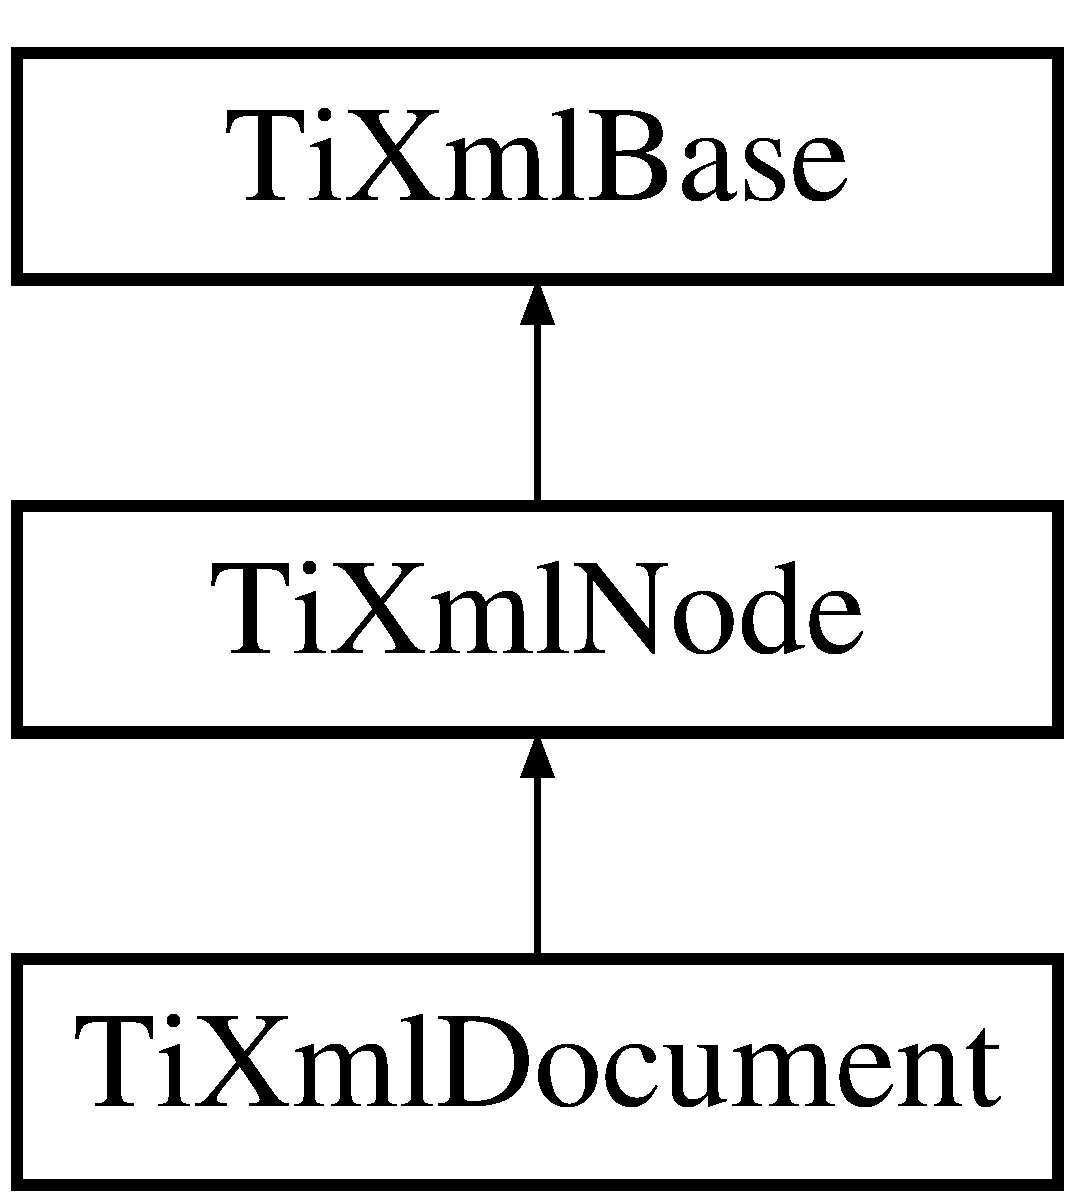
\includegraphics[height=3.000000cm]{class_ti_xml_document}
\end{center}
\end{figure}
\subsection*{Public Member Functions}
\begin{DoxyCompactItemize}
\item 
\hypertarget{class_ti_xml_document_a9f5e84335708fde98400230f9f12659c}{}\label{class_ti_xml_document_a9f5e84335708fde98400230f9f12659c} 
\hyperlink{class_ti_xml_document_a9f5e84335708fde98400230f9f12659c}{Ti\+Xml\+Document} ()
\begin{DoxyCompactList}\small\item\em Create an empty document, that has no name. \end{DoxyCompactList}\item 
\hypertarget{class_ti_xml_document_ae4508b452d0c3061db085f3db27b8396}{}\label{class_ti_xml_document_ae4508b452d0c3061db085f3db27b8396} 
\hyperlink{class_ti_xml_document_ae4508b452d0c3061db085f3db27b8396}{Ti\+Xml\+Document} (const char $\ast$document\+Name)
\begin{DoxyCompactList}\small\item\em Create a document with a name. The name of the document is also the filename of the xml. \end{DoxyCompactList}\item 
\hypertarget{class_ti_xml_document_a2c6e58fb99bfa76cc613f16840022225}{}\label{class_ti_xml_document_a2c6e58fb99bfa76cc613f16840022225} 
\hyperlink{class_ti_xml_document_a2c6e58fb99bfa76cc613f16840022225}{Ti\+Xml\+Document} (const std\+::string \&document\+Name)
\begin{DoxyCompactList}\small\item\em Constructor. \end{DoxyCompactList}\item 
\hypertarget{class_ti_xml_document_a323a7486e7da6099cdc19a5ff7e74b07}{}\label{class_ti_xml_document_a323a7486e7da6099cdc19a5ff7e74b07} 
{\bfseries Ti\+Xml\+Document} (const \hyperlink{class_ti_xml_document}{Ti\+Xml\+Document} \&copy)
\item 
\hypertarget{class_ti_xml_document_aa56fd4dbe8917d2033d865909e2d737e}{}\label{class_ti_xml_document_aa56fd4dbe8917d2033d865909e2d737e} 
\hyperlink{class_ti_xml_document}{Ti\+Xml\+Document} \& {\bfseries operator=} (const \hyperlink{class_ti_xml_document}{Ti\+Xml\+Document} \&copy)
\item 
bool \hyperlink{class_ti_xml_document_a4c852a889c02cf251117fd1d9fe1845f}{Load\+File} (Ti\+Xml\+Encoding encoding=T\+I\+X\+M\+L\+\_\+\+D\+E\+F\+A\+U\+L\+T\+\_\+\+E\+N\+C\+O\+D\+I\+NG)
\item 
\hypertarget{class_ti_xml_document_ab63b96a6af5a467e289c7c75202edad9}{}\label{class_ti_xml_document_ab63b96a6af5a467e289c7c75202edad9} 
bool \hyperlink{class_ti_xml_document_ab63b96a6af5a467e289c7c75202edad9}{Save\+File} () const
\begin{DoxyCompactList}\small\item\em Save a file using the current document value. Returns true if successful. \end{DoxyCompactList}\item 
\hypertarget{class_ti_xml_document_a879cdf5e981b8b2d2ef82f2546dd28fb}{}\label{class_ti_xml_document_a879cdf5e981b8b2d2ef82f2546dd28fb} 
bool \hyperlink{class_ti_xml_document_a879cdf5e981b8b2d2ef82f2546dd28fb}{Load\+File} (const char $\ast$filename, Ti\+Xml\+Encoding encoding=T\+I\+X\+M\+L\+\_\+\+D\+E\+F\+A\+U\+L\+T\+\_\+\+E\+N\+C\+O\+D\+I\+NG)
\begin{DoxyCompactList}\small\item\em Load a file using the given filename. Returns true if successful. \end{DoxyCompactList}\item 
\hypertarget{class_ti_xml_document_ae641f33784381017c44e107cc2c86b5c}{}\label{class_ti_xml_document_ae641f33784381017c44e107cc2c86b5c} 
bool \hyperlink{class_ti_xml_document_ae641f33784381017c44e107cc2c86b5c}{Save\+File} (const char $\ast$filename) const
\begin{DoxyCompactList}\small\item\em Save a file using the given filename. Returns true if successful. \end{DoxyCompactList}\item 
bool \hyperlink{class_ti_xml_document_a41f6fe7200864d1dca663d230caf8db6}{Load\+File} (F\+I\+LE $\ast$, Ti\+Xml\+Encoding encoding=T\+I\+X\+M\+L\+\_\+\+D\+E\+F\+A\+U\+L\+T\+\_\+\+E\+N\+C\+O\+D\+I\+NG)
\item 
\hypertarget{class_ti_xml_document_a8f5a1022168a5767e32becec7b6f44ee}{}\label{class_ti_xml_document_a8f5a1022168a5767e32becec7b6f44ee} 
bool \hyperlink{class_ti_xml_document_a8f5a1022168a5767e32becec7b6f44ee}{Save\+File} (F\+I\+LE $\ast$) const
\begin{DoxyCompactList}\small\item\em Save a file using the given F\+I\+L\+E$\ast$. Returns true if successful. \end{DoxyCompactList}\item 
bool \hyperlink{class_ti_xml_document_a18ae6ed34fed7991ebc220862dfac884}{Load\+File} (const std\+::string \&filename, Ti\+Xml\+Encoding encoding=T\+I\+X\+M\+L\+\_\+\+D\+E\+F\+A\+U\+L\+T\+\_\+\+E\+N\+C\+O\+D\+I\+NG)
\item 
\hypertarget{class_ti_xml_document_a2b3d316ed658852876d4852cd39c42d8}{}\label{class_ti_xml_document_a2b3d316ed658852876d4852cd39c42d8} 
bool \hyperlink{class_ti_xml_document_a2b3d316ed658852876d4852cd39c42d8}{Save\+File} (const std\+::string \&filename) const
\begin{DoxyCompactList}\small\item\em $<$ S\+TL std\+::string version. \end{DoxyCompactList}\item 
virtual const char $\ast$ \hyperlink{class_ti_xml_document_a789ad2f06f93d52bdb5570b2f3670289}{Parse} (const char $\ast$p, \hyperlink{class_ti_xml_parsing_data}{Ti\+Xml\+Parsing\+Data} $\ast$data=0, Ti\+Xml\+Encoding encoding=T\+I\+X\+M\+L\+\_\+\+D\+E\+F\+A\+U\+L\+T\+\_\+\+E\+N\+C\+O\+D\+I\+NG)
\item 
const \hyperlink{class_ti_xml_element}{Ti\+Xml\+Element} $\ast$ \hyperlink{class_ti_xml_document_ab54e3a93279fcf0ac80f06ed9c52f04a}{Root\+Element} () const
\item 
\hypertarget{class_ti_xml_document_a0b43e762a23f938b06651bc90b8a1013}{}\label{class_ti_xml_document_a0b43e762a23f938b06651bc90b8a1013} 
\hyperlink{class_ti_xml_element}{Ti\+Xml\+Element} $\ast$ {\bfseries Root\+Element} ()
\item 
bool \hyperlink{class_ti_xml_document_a348e68faad4a3498f413c51ee9bc321a}{Error} () const
\item 
\hypertarget{class_ti_xml_document_aab511be262e84a003e3bb86f0215c8c2}{}\label{class_ti_xml_document_aab511be262e84a003e3bb86f0215c8c2} 
const char $\ast$ \hyperlink{class_ti_xml_document_aab511be262e84a003e3bb86f0215c8c2}{Error\+Desc} () const
\begin{DoxyCompactList}\small\item\em Contains a textual (english) description of the error if one occurs. \end{DoxyCompactList}\item 
int \hyperlink{class_ti_xml_document_abd928b49a646c8ed53e0453c555d96a2}{Error\+Id} () const
\item 
int \hyperlink{class_ti_xml_document_a062e5257128a7da31b0b2e38cd524600}{Error\+Row} () const
\item 
\hypertarget{class_ti_xml_document_adea69de889449a2587afb8ee043f43f5}{}\label{class_ti_xml_document_adea69de889449a2587afb8ee043f43f5} 
int \hyperlink{class_ti_xml_document_adea69de889449a2587afb8ee043f43f5}{Error\+Col} () const
\begin{DoxyCompactList}\small\item\em The column where the error occured. See \hyperlink{class_ti_xml_document_a062e5257128a7da31b0b2e38cd524600}{Error\+Row()} \end{DoxyCompactList}\item 
void \hyperlink{class_ti_xml_document_a51dac56316f89b35bdb7d0d433ba988e}{Set\+Tab\+Size} (int \+\_\+tabsize)
\item 
\hypertarget{class_ti_xml_document_a81e6ffeee8f5d025a171eabf79abdad7}{}\label{class_ti_xml_document_a81e6ffeee8f5d025a171eabf79abdad7} 
int {\bfseries Tab\+Size} () const
\item 
void \hyperlink{class_ti_xml_document_ac66b8c28db86363315712a3574e87c35}{Clear\+Error} ()
\item 
void \hyperlink{class_ti_xml_document_aa4e8c1498a76dcde7191c683e1220882}{Print} () const
\item 
\hypertarget{class_ti_xml_document_aa9e166fae51da603641380a964f21eeb}{}\label{class_ti_xml_document_aa9e166fae51da603641380a964f21eeb} 
virtual void \hyperlink{class_ti_xml_document_aa9e166fae51da603641380a964f21eeb}{Print} (F\+I\+LE $\ast$cfile, int depth=0) const
\begin{DoxyCompactList}\small\item\em Print this Document to a F\+I\+LE stream. \end{DoxyCompactList}\item 
\hypertarget{class_ti_xml_document_a735c23e318597b920c94eae77fa206de}{}\label{class_ti_xml_document_a735c23e318597b920c94eae77fa206de} 
void {\bfseries Set\+Error} (int err, const char $\ast$error\+Location, \hyperlink{class_ti_xml_parsing_data}{Ti\+Xml\+Parsing\+Data} $\ast$prev\+Data, Ti\+Xml\+Encoding encoding)
\item 
\hypertarget{class_ti_xml_document_a468e582640e3c4f740f7168d8b4a6e4a}{}\label{class_ti_xml_document_a468e582640e3c4f740f7168d8b4a6e4a} 
virtual const \hyperlink{class_ti_xml_document}{Ti\+Xml\+Document} $\ast$ \hyperlink{class_ti_xml_document_a468e582640e3c4f740f7168d8b4a6e4a}{To\+Document} () const
\begin{DoxyCompactList}\small\item\em Cast to a more defined type. Will return null not of the requested type. \end{DoxyCompactList}\item 
\hypertarget{class_ti_xml_document_a1025d942a1f328fd742d545e37efdd42}{}\label{class_ti_xml_document_a1025d942a1f328fd742d545e37efdd42} 
virtual \hyperlink{class_ti_xml_document}{Ti\+Xml\+Document} $\ast$ \hyperlink{class_ti_xml_document_a1025d942a1f328fd742d545e37efdd42}{To\+Document} ()
\begin{DoxyCompactList}\small\item\em Cast to a more defined type. Will return null not of the requested type. \end{DoxyCompactList}\item 
virtual bool \hyperlink{class_ti_xml_document_a8ddd6eec722cbd25900bbac664909bac}{Accept} (\hyperlink{class_ti_xml_visitor}{Ti\+Xml\+Visitor} $\ast$content) const
\end{DoxyCompactItemize}
\subsection*{Protected Member Functions}
\begin{DoxyCompactItemize}
\item 
virtual \hyperlink{class_ti_xml_node}{Ti\+Xml\+Node} $\ast$ \hyperlink{class_ti_xml_document_a46a4dda6c56eb106d46d4046ae1e5353}{Clone} () const
\item 
\hypertarget{class_ti_xml_document_aceaada9ac29206fb660e0449c92b1295}{}\label{class_ti_xml_document_aceaada9ac29206fb660e0449c92b1295} 
virtual void {\bfseries Stream\+In} (std\+::istream $\ast$in, T\+I\+X\+M\+L\+\_\+\+S\+T\+R\+I\+NG $\ast$tag)
\end{DoxyCompactItemize}
\subsection*{Additional Inherited Members}


\subsection{Detailed Description}
Always the top level node. A document binds together all the X\+ML pieces. It can be saved, loaded, and printed to the screen. The \textquotesingle{}value\textquotesingle{} of a document node is the xml file name. 

\subsection{Member Function Documentation}
\hypertarget{class_ti_xml_document_a8ddd6eec722cbd25900bbac664909bac}{}\label{class_ti_xml_document_a8ddd6eec722cbd25900bbac664909bac} 
\index{Ti\+Xml\+Document@{Ti\+Xml\+Document}!Accept@{Accept}}
\index{Accept@{Accept}!Ti\+Xml\+Document@{Ti\+Xml\+Document}}
\subsubsection{\texorpdfstring{Accept()}{Accept()}}
{\footnotesize\ttfamily bool Ti\+Xml\+Document\+::\+Accept (\begin{DoxyParamCaption}\item[{\hyperlink{class_ti_xml_visitor}{Ti\+Xml\+Visitor} $\ast$}]{content }\end{DoxyParamCaption}) const\hspace{0.3cm}{\ttfamily [virtual]}}

Walk the X\+ML tree visiting this node and all of its children. 

Implements \hyperlink{class_ti_xml_node_acc0f88b7462c6cb73809d410a4f5bb86}{Ti\+Xml\+Node}.

\hypertarget{class_ti_xml_document_ac66b8c28db86363315712a3574e87c35}{}\label{class_ti_xml_document_ac66b8c28db86363315712a3574e87c35} 
\index{Ti\+Xml\+Document@{Ti\+Xml\+Document}!Clear\+Error@{Clear\+Error}}
\index{Clear\+Error@{Clear\+Error}!Ti\+Xml\+Document@{Ti\+Xml\+Document}}
\subsubsection{\texorpdfstring{Clear\+Error()}{ClearError()}}
{\footnotesize\ttfamily void Ti\+Xml\+Document\+::\+Clear\+Error (\begin{DoxyParamCaption}{ }\end{DoxyParamCaption})\hspace{0.3cm}{\ttfamily [inline]}}

If you have handled the error, it can be reset with this call. The error state is automatically cleared if you Parse a new X\+ML block. \hypertarget{class_ti_xml_document_a46a4dda6c56eb106d46d4046ae1e5353}{}\label{class_ti_xml_document_a46a4dda6c56eb106d46d4046ae1e5353} 
\index{Ti\+Xml\+Document@{Ti\+Xml\+Document}!Clone@{Clone}}
\index{Clone@{Clone}!Ti\+Xml\+Document@{Ti\+Xml\+Document}}
\subsubsection{\texorpdfstring{Clone()}{Clone()}}
{\footnotesize\ttfamily \hyperlink{class_ti_xml_node}{Ti\+Xml\+Node} $\ast$ Ti\+Xml\+Document\+::\+Clone (\begin{DoxyParamCaption}{ }\end{DoxyParamCaption}) const\hspace{0.3cm}{\ttfamily [protected]}, {\ttfamily [virtual]}}

Create an exact duplicate of this node and return it. The memory must be deleted by the caller. 

Implements \hyperlink{class_ti_xml_node_a4508cc3a2d7a98e96a54cc09c37a78a4}{Ti\+Xml\+Node}.

\hypertarget{class_ti_xml_document_a348e68faad4a3498f413c51ee9bc321a}{}\label{class_ti_xml_document_a348e68faad4a3498f413c51ee9bc321a} 
\index{Ti\+Xml\+Document@{Ti\+Xml\+Document}!Error@{Error}}
\index{Error@{Error}!Ti\+Xml\+Document@{Ti\+Xml\+Document}}
\subsubsection{\texorpdfstring{Error()}{Error()}}
{\footnotesize\ttfamily bool Ti\+Xml\+Document\+::\+Error (\begin{DoxyParamCaption}{ }\end{DoxyParamCaption}) const\hspace{0.3cm}{\ttfamily [inline]}}

If an error occurs, Error will be set to true. Also,
\begin{DoxyItemize}
\item The \hyperlink{class_ti_xml_document_abd928b49a646c8ed53e0453c555d96a2}{Error\+Id()} will contain the integer identifier of the error (not generally useful)
\item The \hyperlink{class_ti_xml_document_aab511be262e84a003e3bb86f0215c8c2}{Error\+Desc()} method will return the name of the error. (very useful)
\item The \hyperlink{class_ti_xml_document_a062e5257128a7da31b0b2e38cd524600}{Error\+Row()} and \hyperlink{class_ti_xml_document_adea69de889449a2587afb8ee043f43f5}{Error\+Col()} will return the location of the error (if known) 
\end{DoxyItemize}\hypertarget{class_ti_xml_document_abd928b49a646c8ed53e0453c555d96a2}{}\label{class_ti_xml_document_abd928b49a646c8ed53e0453c555d96a2} 
\index{Ti\+Xml\+Document@{Ti\+Xml\+Document}!Error\+Id@{Error\+Id}}
\index{Error\+Id@{Error\+Id}!Ti\+Xml\+Document@{Ti\+Xml\+Document}}
\subsubsection{\texorpdfstring{Error\+Id()}{ErrorId()}}
{\footnotesize\ttfamily int Ti\+Xml\+Document\+::\+Error\+Id (\begin{DoxyParamCaption}{ }\end{DoxyParamCaption}) const\hspace{0.3cm}{\ttfamily [inline]}}

Generally, you probably want the error string ( \hyperlink{class_ti_xml_document_aab511be262e84a003e3bb86f0215c8c2}{Error\+Desc()} ). But if you prefer the Error\+Id, this function will fetch it. \hypertarget{class_ti_xml_document_a062e5257128a7da31b0b2e38cd524600}{}\label{class_ti_xml_document_a062e5257128a7da31b0b2e38cd524600} 
\index{Ti\+Xml\+Document@{Ti\+Xml\+Document}!Error\+Row@{Error\+Row}}
\index{Error\+Row@{Error\+Row}!Ti\+Xml\+Document@{Ti\+Xml\+Document}}
\subsubsection{\texorpdfstring{Error\+Row()}{ErrorRow()}}
{\footnotesize\ttfamily int Ti\+Xml\+Document\+::\+Error\+Row (\begin{DoxyParamCaption}{ }\end{DoxyParamCaption}) const\hspace{0.3cm}{\ttfamily [inline]}}

Returns the location (if known) of the error. The first column is column 1, and the first row is row 1. A value of 0 means the row and column wasn\textquotesingle{}t applicable (memory errors, for example, have no row/column) or the parser lost the error. (An error in the error reporting, in that case.)

\begin{DoxySeeAlso}{See also}
\hyperlink{class_ti_xml_document_a51dac56316f89b35bdb7d0d433ba988e}{Set\+Tab\+Size}, \hyperlink{class_ti_xml_base_ad0cacca5d76d156b26511f46080b442e}{Row}, \hyperlink{class_ti_xml_base_ad283b95d9858d5d78c334f4a61b07bb4}{Column} 
\end{DoxySeeAlso}
\hypertarget{class_ti_xml_document_a4c852a889c02cf251117fd1d9fe1845f}{}\label{class_ti_xml_document_a4c852a889c02cf251117fd1d9fe1845f} 
\index{Ti\+Xml\+Document@{Ti\+Xml\+Document}!Load\+File@{Load\+File}}
\index{Load\+File@{Load\+File}!Ti\+Xml\+Document@{Ti\+Xml\+Document}}
\subsubsection{\texorpdfstring{Load\+File()}{LoadFile()}\hspace{0.1cm}{\footnotesize\ttfamily [1/3]}}
{\footnotesize\ttfamily bool Ti\+Xml\+Document\+::\+Load\+File (\begin{DoxyParamCaption}\item[{Ti\+Xml\+Encoding}]{encoding = {\ttfamily TIXML\+\_\+DEFAULT\+\_\+ENCODING} }\end{DoxyParamCaption})}

Load a file using the current document value. Returns true if successful. Will delete any existing document data before loading. \hypertarget{class_ti_xml_document_a41f6fe7200864d1dca663d230caf8db6}{}\label{class_ti_xml_document_a41f6fe7200864d1dca663d230caf8db6} 
\index{Ti\+Xml\+Document@{Ti\+Xml\+Document}!Load\+File@{Load\+File}}
\index{Load\+File@{Load\+File}!Ti\+Xml\+Document@{Ti\+Xml\+Document}}
\subsubsection{\texorpdfstring{Load\+File()}{LoadFile()}\hspace{0.1cm}{\footnotesize\ttfamily [2/3]}}
{\footnotesize\ttfamily bool Ti\+Xml\+Document\+::\+Load\+File (\begin{DoxyParamCaption}\item[{F\+I\+LE $\ast$}]{file,  }\item[{Ti\+Xml\+Encoding}]{encoding = {\ttfamily TIXML\+\_\+DEFAULT\+\_\+ENCODING} }\end{DoxyParamCaption})}

Load a file using the given F\+I\+L\+E$\ast$. Returns true if successful. Note that this method doesn\textquotesingle{}t stream -\/ the entire object pointed at by the F\+I\+L\+E$\ast$ will be interpreted as an X\+ML file. Tiny\+X\+ML doesn\textquotesingle{}t stream in X\+ML from the current file location. Streaming may be added in the future. \hypertarget{class_ti_xml_document_a18ae6ed34fed7991ebc220862dfac884}{}\label{class_ti_xml_document_a18ae6ed34fed7991ebc220862dfac884} 
\index{Ti\+Xml\+Document@{Ti\+Xml\+Document}!Load\+File@{Load\+File}}
\index{Load\+File@{Load\+File}!Ti\+Xml\+Document@{Ti\+Xml\+Document}}
\subsubsection{\texorpdfstring{Load\+File()}{LoadFile()}\hspace{0.1cm}{\footnotesize\ttfamily [3/3]}}
{\footnotesize\ttfamily bool Ti\+Xml\+Document\+::\+Load\+File (\begin{DoxyParamCaption}\item[{const std\+::string \&}]{filename,  }\item[{Ti\+Xml\+Encoding}]{encoding = {\ttfamily TIXML\+\_\+DEFAULT\+\_\+ENCODING} }\end{DoxyParamCaption})\hspace{0.3cm}{\ttfamily [inline]}}


\begin{DoxyParams}{Parameters}
{\em encoding} & S\+TL std\+::string version. \\
\hline
\end{DoxyParams}
\hypertarget{class_ti_xml_document_a789ad2f06f93d52bdb5570b2f3670289}{}\label{class_ti_xml_document_a789ad2f06f93d52bdb5570b2f3670289} 
\index{Ti\+Xml\+Document@{Ti\+Xml\+Document}!Parse@{Parse}}
\index{Parse@{Parse}!Ti\+Xml\+Document@{Ti\+Xml\+Document}}
\subsubsection{\texorpdfstring{Parse()}{Parse()}}
{\footnotesize\ttfamily const char $\ast$ Ti\+Xml\+Document\+::\+Parse (\begin{DoxyParamCaption}\item[{const char $\ast$}]{p,  }\item[{\hyperlink{class_ti_xml_parsing_data}{Ti\+Xml\+Parsing\+Data} $\ast$}]{data = {\ttfamily 0},  }\item[{Ti\+Xml\+Encoding}]{encoding = {\ttfamily TIXML\+\_\+DEFAULT\+\_\+ENCODING} }\end{DoxyParamCaption})\hspace{0.3cm}{\ttfamily [virtual]}}

Parse the given null terminated block of xml data. Passing in an encoding to this method (either T\+I\+X\+M\+L\+\_\+\+E\+N\+C\+O\+D\+I\+N\+G\+\_\+\+L\+E\+G\+A\+CY or T\+I\+X\+M\+L\+\_\+\+E\+N\+C\+O\+D\+I\+N\+G\+\_\+\+U\+T\+F8 will force Tiny\+Xml to use that encoding, regardless of what Tiny\+Xml might otherwise try to detect. 

Implements \hyperlink{class_ti_xml_base}{Ti\+Xml\+Base}.

\hypertarget{class_ti_xml_document_aa4e8c1498a76dcde7191c683e1220882}{}\label{class_ti_xml_document_aa4e8c1498a76dcde7191c683e1220882} 
\index{Ti\+Xml\+Document@{Ti\+Xml\+Document}!Print@{Print}}
\index{Print@{Print}!Ti\+Xml\+Document@{Ti\+Xml\+Document}}
\subsubsection{\texorpdfstring{Print()}{Print()}}
{\footnotesize\ttfamily void Ti\+Xml\+Document\+::\+Print (\begin{DoxyParamCaption}{ }\end{DoxyParamCaption}) const\hspace{0.3cm}{\ttfamily [inline]}}

Write the document to standard out using formatted printing (\char`\"{}pretty print\char`\"{}). \hypertarget{class_ti_xml_document_ab54e3a93279fcf0ac80f06ed9c52f04a}{}\label{class_ti_xml_document_ab54e3a93279fcf0ac80f06ed9c52f04a} 
\index{Ti\+Xml\+Document@{Ti\+Xml\+Document}!Root\+Element@{Root\+Element}}
\index{Root\+Element@{Root\+Element}!Ti\+Xml\+Document@{Ti\+Xml\+Document}}
\subsubsection{\texorpdfstring{Root\+Element()}{RootElement()}}
{\footnotesize\ttfamily const \hyperlink{class_ti_xml_element}{Ti\+Xml\+Element}$\ast$ Ti\+Xml\+Document\+::\+Root\+Element (\begin{DoxyParamCaption}{ }\end{DoxyParamCaption}) const\hspace{0.3cm}{\ttfamily [inline]}}

Get the root element -- the only top level element -- of the document. In well formed X\+ML, there should only be one. Tiny\+Xml is tolerant of multiple elements at the document level. \hypertarget{class_ti_xml_document_a51dac56316f89b35bdb7d0d433ba988e}{}\label{class_ti_xml_document_a51dac56316f89b35bdb7d0d433ba988e} 
\index{Ti\+Xml\+Document@{Ti\+Xml\+Document}!Set\+Tab\+Size@{Set\+Tab\+Size}}
\index{Set\+Tab\+Size@{Set\+Tab\+Size}!Ti\+Xml\+Document@{Ti\+Xml\+Document}}
\subsubsection{\texorpdfstring{Set\+Tab\+Size()}{SetTabSize()}}
{\footnotesize\ttfamily void Ti\+Xml\+Document\+::\+Set\+Tab\+Size (\begin{DoxyParamCaption}\item[{int}]{\+\_\+tabsize }\end{DoxyParamCaption})\hspace{0.3cm}{\ttfamily [inline]}}

\hyperlink{class_ti_xml_document_a51dac56316f89b35bdb7d0d433ba988e}{Set\+Tab\+Size()} allows the error reporting functions (\hyperlink{class_ti_xml_document_a062e5257128a7da31b0b2e38cd524600}{Error\+Row()} and \hyperlink{class_ti_xml_document_adea69de889449a2587afb8ee043f43f5}{Error\+Col()}) to report the correct values for row and column. It does not change the output or input in any way.

By calling this method, with a tab size greater than 0, the row and column of each node and attribute is stored when the file is loaded. Very useful for tracking the D\+OM back in to the source file.

The tab size is required for calculating the location of nodes. If not set, the default of 4 is used. The tabsize is set per document. Setting the tabsize to 0 disables row/column tracking.

Note that row and column tracking is not supported when using operator$>$$>$.

The tab size needs to be enabled before the parse or load. Correct usage\+: \begin{DoxyVerb}TiXmlDocument doc;
doc.SetTabSize( 8 );
doc.Load( "myfile.xml" );
\end{DoxyVerb}


\begin{DoxySeeAlso}{See also}
\hyperlink{class_ti_xml_base_ad0cacca5d76d156b26511f46080b442e}{Row}, \hyperlink{class_ti_xml_base_ad283b95d9858d5d78c334f4a61b07bb4}{Column} 
\end{DoxySeeAlso}


The documentation for this class was generated from the following files\+:\begin{DoxyCompactItemize}
\item 
utility/tiny\+\_\+xml/tinyxml.\+h\item 
utility/tiny\+\_\+xml/tinyxml.\+cpp\item 
utility/tiny\+\_\+xml/tinyxmlparser.\+cpp\end{DoxyCompactItemize}

\hypertarget{class_ti_xml_element}{}\section{Ti\+Xml\+Element Class Reference}
\label{class_ti_xml_element}\index{Ti\+Xml\+Element@{Ti\+Xml\+Element}}


{\ttfamily \#include $<$tinyxml.\+h$>$}

Inheritance diagram for Ti\+Xml\+Element\+:\begin{figure}[H]
\begin{center}
\leavevmode
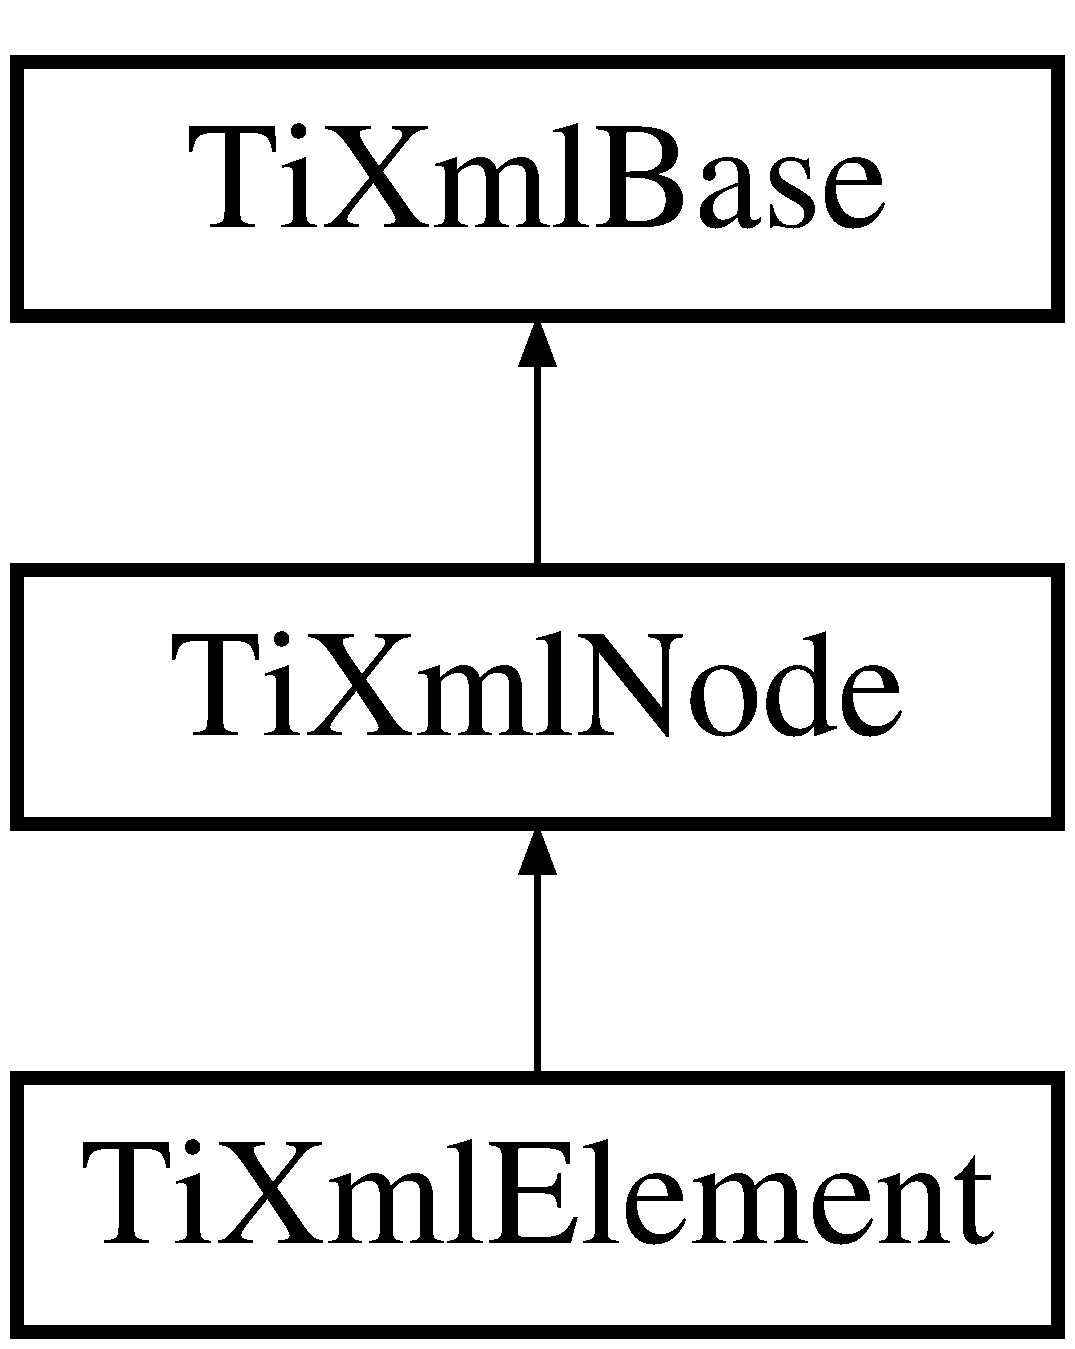
\includegraphics[height=3.000000cm]{class_ti_xml_element}
\end{center}
\end{figure}
\subsection*{Public Member Functions}
\begin{DoxyCompactItemize}
\item 
\mbox{\Hypertarget{class_ti_xml_element_a01bc3ab372d35da08efcbbe65ad90c60}\label{class_ti_xml_element_a01bc3ab372d35da08efcbbe65ad90c60}} 
\hyperlink{class_ti_xml_element_a01bc3ab372d35da08efcbbe65ad90c60}{Ti\+Xml\+Element} (const char $\ast$in\+\_\+value)
\begin{DoxyCompactList}\small\item\em Construct an element. \end{DoxyCompactList}\item 
\mbox{\Hypertarget{class_ti_xml_element_a40fc2e3c1a955e2f78e1a32350d180e7}\label{class_ti_xml_element_a40fc2e3c1a955e2f78e1a32350d180e7}} 
\hyperlink{class_ti_xml_element_a40fc2e3c1a955e2f78e1a32350d180e7}{Ti\+Xml\+Element} (const std\+::string \&\+\_\+value)
\begin{DoxyCompactList}\small\item\em std\+::string constructor. \end{DoxyCompactList}\item 
\mbox{\Hypertarget{class_ti_xml_element_a1ca4465f3c2eac6a60e641cd7f1d9f7e}\label{class_ti_xml_element_a1ca4465f3c2eac6a60e641cd7f1d9f7e}} 
{\bfseries Ti\+Xml\+Element} (const \hyperlink{class_ti_xml_element}{Ti\+Xml\+Element} \&)
\item 
\mbox{\Hypertarget{class_ti_xml_element_ad58d300f4cfc0016ffa6861ebb718a0b}\label{class_ti_xml_element_ad58d300f4cfc0016ffa6861ebb718a0b}} 
\hyperlink{class_ti_xml_element}{Ti\+Xml\+Element} \& {\bfseries operator=} (const \hyperlink{class_ti_xml_element}{Ti\+Xml\+Element} \&base)
\item 
const char $\ast$ \hyperlink{class_ti_xml_element_a6042f518748f475a7ac4b4e0b509eb05}{Attribute} (const char $\ast$name) const
\item 
const char $\ast$ \hyperlink{class_ti_xml_element_a8005d0b808fd02bd1246710cdf95e5f6}{Attribute} (const char $\ast$name, int $\ast$i) const
\item 
const char $\ast$ \hyperlink{class_ti_xml_element_a09df893402d0ab1402c8725e6d30ec04}{Attribute} (const char $\ast$name, double $\ast$d) const
\item 
int \hyperlink{class_ti_xml_element_a5c0f739e0f6f5905a201364532e54a60}{Query\+Int\+Attribute} (const char $\ast$name, int $\ast$\+\_\+value) const
\item 
\mbox{\Hypertarget{class_ti_xml_element_ab75c83543d4ace62f4c40d7e8e392fc3}\label{class_ti_xml_element_ab75c83543d4ace62f4c40d7e8e392fc3}} 
int \hyperlink{class_ti_xml_element_ab75c83543d4ace62f4c40d7e8e392fc3}{Query\+Unsigned\+Attribute} (const char $\ast$name, unsigned $\ast$\+\_\+value) const
\begin{DoxyCompactList}\small\item\em Query\+Unsigned\+Attribute examines the attribute -\/ see \hyperlink{class_ti_xml_element_a5c0f739e0f6f5905a201364532e54a60}{Query\+Int\+Attribute()}. \end{DoxyCompactList}\item 
int \hyperlink{class_ti_xml_element_a5789b1488af75b6ae37a749700495ceb}{Query\+Bool\+Attribute} (const char $\ast$name, bool $\ast$\+\_\+value) const
\item 
\mbox{\Hypertarget{class_ti_xml_element_ae04bad29ddb281a7e6c662b3882e9928}\label{class_ti_xml_element_ae04bad29ddb281a7e6c662b3882e9928}} 
int \hyperlink{class_ti_xml_element_ae04bad29ddb281a7e6c662b3882e9928}{Query\+Double\+Attribute} (const char $\ast$name, double $\ast$\+\_\+value) const
\begin{DoxyCompactList}\small\item\em Query\+Double\+Attribute examines the attribute -\/ see \hyperlink{class_ti_xml_element_a5c0f739e0f6f5905a201364532e54a60}{Query\+Int\+Attribute()}. \end{DoxyCompactList}\item 
\mbox{\Hypertarget{class_ti_xml_element_a5591929834178699b4561ab6ab460068}\label{class_ti_xml_element_a5591929834178699b4561ab6ab460068}} 
int \hyperlink{class_ti_xml_element_a5591929834178699b4561ab6ab460068}{Query\+Float\+Attribute} (const char $\ast$name, float $\ast$\+\_\+value) const
\begin{DoxyCompactList}\small\item\em Query\+Float\+Attribute examines the attribute -\/ see \hyperlink{class_ti_xml_element_a5c0f739e0f6f5905a201364532e54a60}{Query\+Int\+Attribute()}. \end{DoxyCompactList}\item 
\mbox{\Hypertarget{class_ti_xml_element_afa8f8a62753a440186b5cd28e252a4e4}\label{class_ti_xml_element_afa8f8a62753a440186b5cd28e252a4e4}} 
int \hyperlink{class_ti_xml_element_afa8f8a62753a440186b5cd28e252a4e4}{Query\+String\+Attribute} (const char $\ast$name, std\+::string $\ast$\+\_\+value) const
\begin{DoxyCompactList}\small\item\em Query\+String\+Attribute examines the attribute -\/ see \hyperlink{class_ti_xml_element_a5c0f739e0f6f5905a201364532e54a60}{Query\+Int\+Attribute()}. \end{DoxyCompactList}\item 
{\footnotesize template$<$typename T $>$ }\\int \hyperlink{class_ti_xml_element_a7530db879b81ebaba61bf62a9770d204}{Query\+Value\+Attribute} (const std\+::string \&name, T $\ast$out\+Value) const
\item 
\mbox{\Hypertarget{class_ti_xml_element_aad40c4f4f34f854862e6a719e83ad713}\label{class_ti_xml_element_aad40c4f4f34f854862e6a719e83ad713}} 
int {\bfseries Query\+Value\+Attribute} (const std\+::string \&name, std\+::string $\ast$out\+Value) const
\item 
void \hyperlink{class_ti_xml_element_abf0b3bd7f0e4c746a89ec6e7f101fc32}{Set\+Attribute} (const char $\ast$name, const char $\ast$\+\_\+value)
\item 
\mbox{\Hypertarget{class_ti_xml_element_aa0533e0dc704ce9f38308c9cfbe705e5}\label{class_ti_xml_element_aa0533e0dc704ce9f38308c9cfbe705e5}} 
const std\+::string $\ast$ {\bfseries Attribute} (const std\+::string \&name) const
\item 
\mbox{\Hypertarget{class_ti_xml_element_a88cc395de3e5460bb96a42cb9d5ef096}\label{class_ti_xml_element_a88cc395de3e5460bb96a42cb9d5ef096}} 
const std\+::string $\ast$ {\bfseries Attribute} (const std\+::string \&name, int $\ast$i) const
\item 
\mbox{\Hypertarget{class_ti_xml_element_a4f624b438f8a969df782649ea258c98b}\label{class_ti_xml_element_a4f624b438f8a969df782649ea258c98b}} 
const std\+::string $\ast$ {\bfseries Attribute} (const std\+::string \&name, double $\ast$d) const
\item 
\mbox{\Hypertarget{class_ti_xml_element_aa368685cfa6efae820b8e7ec18114865}\label{class_ti_xml_element_aa368685cfa6efae820b8e7ec18114865}} 
int {\bfseries Query\+Int\+Attribute} (const std\+::string \&name, int $\ast$\+\_\+value) const
\item 
\mbox{\Hypertarget{class_ti_xml_element_a442a0180263ff9a61d30711dc213d9e4}\label{class_ti_xml_element_a442a0180263ff9a61d30711dc213d9e4}} 
int {\bfseries Query\+Double\+Attribute} (const std\+::string \&name, double $\ast$\+\_\+value) const
\item 
void \hyperlink{class_ti_xml_element_a80ed65b1d194c71c6c9986ae42337d7d}{Set\+Attribute} (const std\+::string \&name, const std\+::string \&\+\_\+value)
\begin{DoxyCompactList}\small\item\em S\+TL std\+::string form. \end{DoxyCompactList}\item 
\mbox{\Hypertarget{class_ti_xml_element_a6f18d54fbe25bbc527936ee65363b3c5}\label{class_ti_xml_element_a6f18d54fbe25bbc527936ee65363b3c5}} 
void \hyperlink{class_ti_xml_element_a6f18d54fbe25bbc527936ee65363b3c5}{Set\+Attribute} (const std\+::string \&name, int \+\_\+value)
\begin{DoxyCompactList}\small\item\em S\+TL std\+::string form. \end{DoxyCompactList}\item 
\mbox{\Hypertarget{class_ti_xml_element_ac2112d423b39a93012b241f6baf4d3d3}\label{class_ti_xml_element_ac2112d423b39a93012b241f6baf4d3d3}} 
void {\bfseries Set\+Double\+Attribute} (const std\+::string \&name, double value)
\item 
void \hyperlink{class_ti_xml_element_ace6f4be75e373726d4774073d666d1a7}{Set\+Attribute} (const char $\ast$name, int value)
\item 
void \hyperlink{class_ti_xml_element_a0d1dd975d75496778177e35abfe0ec0b}{Set\+Double\+Attribute} (const char $\ast$name, double value)
\item 
void \hyperlink{class_ti_xml_element_a56979767deca794376b1dfa69a525b2a}{Remove\+Attribute} (const char $\ast$name)
\item 
\mbox{\Hypertarget{class_ti_xml_element_a1afa6aea716511326a608e4c05df4f3a}\label{class_ti_xml_element_a1afa6aea716511326a608e4c05df4f3a}} 
void \hyperlink{class_ti_xml_element_a1afa6aea716511326a608e4c05df4f3a}{Remove\+Attribute} (const std\+::string \&name)
\begin{DoxyCompactList}\small\item\em S\+TL std\+::string form. \end{DoxyCompactList}\item 
\mbox{\Hypertarget{class_ti_xml_element_a003131b1bbf0b8054b11571c1b9a4d3a}\label{class_ti_xml_element_a003131b1bbf0b8054b11571c1b9a4d3a}} 
const \hyperlink{class_ti_xml_attribute}{Ti\+Xml\+Attribute} $\ast$ \hyperlink{class_ti_xml_element_a003131b1bbf0b8054b11571c1b9a4d3a}{First\+Attribute} () const
\begin{DoxyCompactList}\small\item\em Access the first attribute in this element. \end{DoxyCompactList}\item 
\mbox{\Hypertarget{class_ti_xml_element_a4b33780fc565d38d6b54f640e0cf1737}\label{class_ti_xml_element_a4b33780fc565d38d6b54f640e0cf1737}} 
\hyperlink{class_ti_xml_attribute}{Ti\+Xml\+Attribute} $\ast$ {\bfseries First\+Attribute} ()
\item 
\mbox{\Hypertarget{class_ti_xml_element_a42939f55ed4cec5fc1daaecfded7ba16}\label{class_ti_xml_element_a42939f55ed4cec5fc1daaecfded7ba16}} 
const \hyperlink{class_ti_xml_attribute}{Ti\+Xml\+Attribute} $\ast$ \hyperlink{class_ti_xml_element_a42939f55ed4cec5fc1daaecfded7ba16}{Last\+Attribute} () const
\begin{DoxyCompactList}\small\item\em Access the last attribute in this element. \end{DoxyCompactList}\item 
\mbox{\Hypertarget{class_ti_xml_element_a222f81cf06155cd108f2a68d4d176004}\label{class_ti_xml_element_a222f81cf06155cd108f2a68d4d176004}} 
\hyperlink{class_ti_xml_attribute}{Ti\+Xml\+Attribute} $\ast$ {\bfseries Last\+Attribute} ()
\item 
const char $\ast$ \hyperlink{class_ti_xml_element_af0f814ecbd43d50d4cdbdf4354d3da39}{Get\+Text} () const
\item 
\mbox{\Hypertarget{class_ti_xml_element_a810ea8fa40844c01334e5af2a26794cb}\label{class_ti_xml_element_a810ea8fa40844c01334e5af2a26794cb}} 
virtual \hyperlink{class_ti_xml_node}{Ti\+Xml\+Node} $\ast$ \hyperlink{class_ti_xml_element_a810ea8fa40844c01334e5af2a26794cb}{Clone} () const
\begin{DoxyCompactList}\small\item\em Creates a new Element and returns it -\/ the returned element is a copy. \end{DoxyCompactList}\item 
virtual void \hyperlink{class_ti_xml_element_aa31a15cddfb8601a31236fe7d2569fb4}{Print} (F\+I\+LE $\ast$cfile, int depth) const
\item 
\mbox{\Hypertarget{class_ti_xml_element_af95c9165159fd9dfdcc5b894a3fcf85b}\label{class_ti_xml_element_af95c9165159fd9dfdcc5b894a3fcf85b}} 
virtual const char $\ast$ {\bfseries Parse} (const char $\ast$p, \hyperlink{class_ti_xml_parsing_data}{Ti\+Xml\+Parsing\+Data} $\ast$data, Ti\+Xml\+Encoding encoding)
\item 
\mbox{\Hypertarget{class_ti_xml_element_a940fc8aa953e0ef0de6e110b7d98b8ee}\label{class_ti_xml_element_a940fc8aa953e0ef0de6e110b7d98b8ee}} 
virtual const \hyperlink{class_ti_xml_element}{Ti\+Xml\+Element} $\ast$ \hyperlink{class_ti_xml_element_a940fc8aa953e0ef0de6e110b7d98b8ee}{To\+Element} () const
\begin{DoxyCompactList}\small\item\em Cast to a more defined type. Will return null not of the requested type. \end{DoxyCompactList}\item 
\mbox{\Hypertarget{class_ti_xml_element_a9def86337ea7a755eb41cac980f60c7a}\label{class_ti_xml_element_a9def86337ea7a755eb41cac980f60c7a}} 
virtual \hyperlink{class_ti_xml_element}{Ti\+Xml\+Element} $\ast$ \hyperlink{class_ti_xml_element_a9def86337ea7a755eb41cac980f60c7a}{To\+Element} ()
\begin{DoxyCompactList}\small\item\em Cast to a more defined type. Will return null not of the requested type. \end{DoxyCompactList}\item 
virtual bool \hyperlink{class_ti_xml_element_a01d33358cce9d1817b557d314dda3779}{Accept} (\hyperlink{class_ti_xml_visitor}{Ti\+Xml\+Visitor} $\ast$visitor) const
\end{DoxyCompactItemize}
\subsection*{Protected Member Functions}
\begin{DoxyCompactItemize}
\item 
\mbox{\Hypertarget{class_ti_xml_element_ab931f2208ed76ba03465d8a1f86b5935}\label{class_ti_xml_element_ab931f2208ed76ba03465d8a1f86b5935}} 
void {\bfseries Copy\+To} (\hyperlink{class_ti_xml_element}{Ti\+Xml\+Element} $\ast$target) const
\item 
\mbox{\Hypertarget{class_ti_xml_element_a5670933ec2d7d9763b9891acc05d7f7d}\label{class_ti_xml_element_a5670933ec2d7d9763b9891acc05d7f7d}} 
void {\bfseries Clear\+This} ()
\item 
\mbox{\Hypertarget{class_ti_xml_element_a6884b491fb4708dae566f3ddc1476536}\label{class_ti_xml_element_a6884b491fb4708dae566f3ddc1476536}} 
virtual void {\bfseries Stream\+In} (std\+::istream $\ast$in, T\+I\+X\+M\+L\+\_\+\+S\+T\+R\+I\+NG $\ast$tag)
\item 
\mbox{\Hypertarget{class_ti_xml_element_ac786bce103042d3837c4cc2ff6967d41}\label{class_ti_xml_element_ac786bce103042d3837c4cc2ff6967d41}} 
const char $\ast$ {\bfseries Read\+Value} (const char $\ast$in, \hyperlink{class_ti_xml_parsing_data}{Ti\+Xml\+Parsing\+Data} $\ast$prev\+Data, Ti\+Xml\+Encoding encoding)
\end{DoxyCompactItemize}
\subsection*{Additional Inherited Members}


\subsection{Detailed Description}
The element is a container class. It has a value, the element name, and can contain other elements, text, comments, and unknowns. Elements also contain an arbitrary number of attributes. 

\subsection{Member Function Documentation}
\mbox{\Hypertarget{class_ti_xml_element_a01d33358cce9d1817b557d314dda3779}\label{class_ti_xml_element_a01d33358cce9d1817b557d314dda3779}} 
\index{Ti\+Xml\+Element@{Ti\+Xml\+Element}!Accept@{Accept}}
\index{Accept@{Accept}!Ti\+Xml\+Element@{Ti\+Xml\+Element}}
\subsubsection{\texorpdfstring{Accept()}{Accept()}}
{\footnotesize\ttfamily bool Ti\+Xml\+Element\+::\+Accept (\begin{DoxyParamCaption}\item[{\hyperlink{class_ti_xml_visitor}{Ti\+Xml\+Visitor} $\ast$}]{visitor }\end{DoxyParamCaption}) const\hspace{0.3cm}{\ttfamily [virtual]}}

Walk the X\+ML tree visiting this node and all of its children. 

Implements \hyperlink{class_ti_xml_node_acc0f88b7462c6cb73809d410a4f5bb86}{Ti\+Xml\+Node}.

\mbox{\Hypertarget{class_ti_xml_element_a6042f518748f475a7ac4b4e0b509eb05}\label{class_ti_xml_element_a6042f518748f475a7ac4b4e0b509eb05}} 
\index{Ti\+Xml\+Element@{Ti\+Xml\+Element}!Attribute@{Attribute}}
\index{Attribute@{Attribute}!Ti\+Xml\+Element@{Ti\+Xml\+Element}}
\subsubsection{\texorpdfstring{Attribute()}{Attribute()}\hspace{0.1cm}{\footnotesize\ttfamily [1/3]}}
{\footnotesize\ttfamily const char $\ast$ Ti\+Xml\+Element\+::\+Attribute (\begin{DoxyParamCaption}\item[{const char $\ast$}]{name }\end{DoxyParamCaption}) const}

Given an attribute name, \hyperlink{class_ti_xml_element_a6042f518748f475a7ac4b4e0b509eb05}{Attribute()} returns the value for the attribute of that name, or null if none exists. \mbox{\Hypertarget{class_ti_xml_element_a8005d0b808fd02bd1246710cdf95e5f6}\label{class_ti_xml_element_a8005d0b808fd02bd1246710cdf95e5f6}} 
\index{Ti\+Xml\+Element@{Ti\+Xml\+Element}!Attribute@{Attribute}}
\index{Attribute@{Attribute}!Ti\+Xml\+Element@{Ti\+Xml\+Element}}
\subsubsection{\texorpdfstring{Attribute()}{Attribute()}\hspace{0.1cm}{\footnotesize\ttfamily [2/3]}}
{\footnotesize\ttfamily const char $\ast$ Ti\+Xml\+Element\+::\+Attribute (\begin{DoxyParamCaption}\item[{const char $\ast$}]{name,  }\item[{int $\ast$}]{i }\end{DoxyParamCaption}) const}

Given an attribute name, \hyperlink{class_ti_xml_element_a6042f518748f475a7ac4b4e0b509eb05}{Attribute()} returns the value for the attribute of that name, or null if none exists. If the attribute exists and can be converted to an integer, the integer value will be put in the return \textquotesingle{}i\textquotesingle{}, if \textquotesingle{}i\textquotesingle{} is non-\/null. \mbox{\Hypertarget{class_ti_xml_element_a09df893402d0ab1402c8725e6d30ec04}\label{class_ti_xml_element_a09df893402d0ab1402c8725e6d30ec04}} 
\index{Ti\+Xml\+Element@{Ti\+Xml\+Element}!Attribute@{Attribute}}
\index{Attribute@{Attribute}!Ti\+Xml\+Element@{Ti\+Xml\+Element}}
\subsubsection{\texorpdfstring{Attribute()}{Attribute()}\hspace{0.1cm}{\footnotesize\ttfamily [3/3]}}
{\footnotesize\ttfamily const char $\ast$ Ti\+Xml\+Element\+::\+Attribute (\begin{DoxyParamCaption}\item[{const char $\ast$}]{name,  }\item[{double $\ast$}]{d }\end{DoxyParamCaption}) const}

Given an attribute name, \hyperlink{class_ti_xml_element_a6042f518748f475a7ac4b4e0b509eb05}{Attribute()} returns the value for the attribute of that name, or null if none exists. If the attribute exists and can be converted to an double, the double value will be put in the return \textquotesingle{}d\textquotesingle{}, if \textquotesingle{}d\textquotesingle{} is non-\/null. \mbox{\Hypertarget{class_ti_xml_element_af0f814ecbd43d50d4cdbdf4354d3da39}\label{class_ti_xml_element_af0f814ecbd43d50d4cdbdf4354d3da39}} 
\index{Ti\+Xml\+Element@{Ti\+Xml\+Element}!Get\+Text@{Get\+Text}}
\index{Get\+Text@{Get\+Text}!Ti\+Xml\+Element@{Ti\+Xml\+Element}}
\subsubsection{\texorpdfstring{Get\+Text()}{GetText()}}
{\footnotesize\ttfamily const char $\ast$ Ti\+Xml\+Element\+::\+Get\+Text (\begin{DoxyParamCaption}{ }\end{DoxyParamCaption}) const}

Convenience function for easy access to the text inside an element. Although easy and concise, \hyperlink{class_ti_xml_element_af0f814ecbd43d50d4cdbdf4354d3da39}{Get\+Text()} is limited compared to getting the \hyperlink{class_ti_xml_text}{Ti\+Xml\+Text} child and accessing it directly.

If the first child of \textquotesingle{}this\textquotesingle{} is a \hyperlink{class_ti_xml_text}{Ti\+Xml\+Text}, the \hyperlink{class_ti_xml_element_af0f814ecbd43d50d4cdbdf4354d3da39}{Get\+Text()} returns the character string of the Text node, else null is returned.

This is a convenient method for getting the text of simple contained text\+: \begin{DoxyVerb}<foo>This is text</foo>
const char* str = fooElement->GetText();
\end{DoxyVerb}


\textquotesingle{}str\textquotesingle{} will be a pointer to \char`\"{}\+This is text\char`\"{}.

Note that this function can be misleading. If the element foo was created from this X\+ML\+: \begin{DoxyVerb}<foo><b>This is text</b></foo> 
\end{DoxyVerb}


then the value of str would be null. The first child node isn\textquotesingle{}t a text node, it is another element. From this X\+ML\+: \begin{DoxyVerb}<foo>This is <b>text</b></foo> 
\end{DoxyVerb}
 \hyperlink{class_ti_xml_element_af0f814ecbd43d50d4cdbdf4354d3da39}{Get\+Text()} will return \char`\"{}\+This is \char`\"{}.

W\+A\+R\+N\+I\+NG\+: \hyperlink{class_ti_xml_element_af0f814ecbd43d50d4cdbdf4354d3da39}{Get\+Text()} accesses a child node -\/ don\textquotesingle{}t become confused with the similarly named \hyperlink{class_ti_xml_handle_ad3b502c72059421e4dfcc7bda3c392fe}{Ti\+Xml\+Handle\+::\+Text()} and \hyperlink{class_ti_xml_node_a3ddfbcac78fbea041fad57e5c6d60a03}{Ti\+Xml\+Node\+::\+To\+Text()} which are safe type casts on the referenced node. \mbox{\Hypertarget{class_ti_xml_element_aa31a15cddfb8601a31236fe7d2569fb4}\label{class_ti_xml_element_aa31a15cddfb8601a31236fe7d2569fb4}} 
\index{Ti\+Xml\+Element@{Ti\+Xml\+Element}!Print@{Print}}
\index{Print@{Print}!Ti\+Xml\+Element@{Ti\+Xml\+Element}}
\subsubsection{\texorpdfstring{Print()}{Print()}}
{\footnotesize\ttfamily void Ti\+Xml\+Element\+::\+Print (\begin{DoxyParamCaption}\item[{F\+I\+LE $\ast$}]{cfile,  }\item[{int}]{depth }\end{DoxyParamCaption}) const\hspace{0.3cm}{\ttfamily [virtual]}}

All Tiny\+Xml classes can print themselves to a filestream or the string class (\hyperlink{class_ti_xml_string}{Ti\+Xml\+String} in non-\/\+S\+TL mode, std\+::string in S\+TL mode.) Either or both cfile and str can be null.

This is a formatted print, and will insert tabs and newlines.

(For an unformatted stream, use the $<$$<$ operator.) 

Implements \hyperlink{class_ti_xml_base_a0de56b3f2ef14c65091a3b916437b512}{Ti\+Xml\+Base}.

\mbox{\Hypertarget{class_ti_xml_element_a5789b1488af75b6ae37a749700495ceb}\label{class_ti_xml_element_a5789b1488af75b6ae37a749700495ceb}} 
\index{Ti\+Xml\+Element@{Ti\+Xml\+Element}!Query\+Bool\+Attribute@{Query\+Bool\+Attribute}}
\index{Query\+Bool\+Attribute@{Query\+Bool\+Attribute}!Ti\+Xml\+Element@{Ti\+Xml\+Element}}
\subsubsection{\texorpdfstring{Query\+Bool\+Attribute()}{QueryBoolAttribute()}}
{\footnotesize\ttfamily int Ti\+Xml\+Element\+::\+Query\+Bool\+Attribute (\begin{DoxyParamCaption}\item[{const char $\ast$}]{name,  }\item[{bool $\ast$}]{\+\_\+value }\end{DoxyParamCaption}) const}

Query\+Bool\+Attribute examines the attribute -\/ see \hyperlink{class_ti_xml_element_a5c0f739e0f6f5905a201364532e54a60}{Query\+Int\+Attribute()}. Note that \textquotesingle{}1\textquotesingle{}, \textquotesingle{}true\textquotesingle{}, or \textquotesingle{}yes\textquotesingle{} are considered true, while \textquotesingle{}0\textquotesingle{}, \textquotesingle{}false\textquotesingle{} and \textquotesingle{}no\textquotesingle{} are considered false. \mbox{\Hypertarget{class_ti_xml_element_a5c0f739e0f6f5905a201364532e54a60}\label{class_ti_xml_element_a5c0f739e0f6f5905a201364532e54a60}} 
\index{Ti\+Xml\+Element@{Ti\+Xml\+Element}!Query\+Int\+Attribute@{Query\+Int\+Attribute}}
\index{Query\+Int\+Attribute@{Query\+Int\+Attribute}!Ti\+Xml\+Element@{Ti\+Xml\+Element}}
\subsubsection{\texorpdfstring{Query\+Int\+Attribute()}{QueryIntAttribute()}}
{\footnotesize\ttfamily int Ti\+Xml\+Element\+::\+Query\+Int\+Attribute (\begin{DoxyParamCaption}\item[{const char $\ast$}]{name,  }\item[{int $\ast$}]{\+\_\+value }\end{DoxyParamCaption}) const}

Query\+Int\+Attribute examines the attribute -\/ it is an alternative to the \hyperlink{class_ti_xml_element_a6042f518748f475a7ac4b4e0b509eb05}{Attribute()} method with richer error checking. If the attribute is an integer, it is stored in \textquotesingle{}value\textquotesingle{} and the call returns T\+I\+X\+M\+L\+\_\+\+S\+U\+C\+C\+E\+SS. If it is not an integer, it returns T\+I\+X\+M\+L\+\_\+\+W\+R\+O\+N\+G\+\_\+\+T\+Y\+PE. If the attribute does not exist, then T\+I\+X\+M\+L\+\_\+\+N\+O\+\_\+\+A\+T\+T\+R\+I\+B\+U\+TE is returned. \mbox{\Hypertarget{class_ti_xml_element_a7530db879b81ebaba61bf62a9770d204}\label{class_ti_xml_element_a7530db879b81ebaba61bf62a9770d204}} 
\index{Ti\+Xml\+Element@{Ti\+Xml\+Element}!Query\+Value\+Attribute@{Query\+Value\+Attribute}}
\index{Query\+Value\+Attribute@{Query\+Value\+Attribute}!Ti\+Xml\+Element@{Ti\+Xml\+Element}}
\subsubsection{\texorpdfstring{Query\+Value\+Attribute()}{QueryValueAttribute()}}
{\footnotesize\ttfamily template$<$typename T $>$ \\
int Ti\+Xml\+Element\+::\+Query\+Value\+Attribute (\begin{DoxyParamCaption}\item[{const std\+::string \&}]{name,  }\item[{T $\ast$}]{out\+Value }\end{DoxyParamCaption}) const\hspace{0.3cm}{\ttfamily [inline]}}

Template form of the attribute query which will try to read the attribute into the specified type. Very easy, very powerful, but be careful to make sure to call this with the correct type.

N\+O\+TE\+: This method doesn\textquotesingle{}t work correctly for \textquotesingle{}string\textquotesingle{} types that contain spaces.

\begin{DoxyReturn}{Returns}
T\+I\+X\+M\+L\+\_\+\+S\+U\+C\+C\+E\+SS, T\+I\+X\+M\+L\+\_\+\+W\+R\+O\+N\+G\+\_\+\+T\+Y\+PE, or T\+I\+X\+M\+L\+\_\+\+N\+O\+\_\+\+A\+T\+T\+R\+I\+B\+U\+TE 
\end{DoxyReturn}
\mbox{\Hypertarget{class_ti_xml_element_a56979767deca794376b1dfa69a525b2a}\label{class_ti_xml_element_a56979767deca794376b1dfa69a525b2a}} 
\index{Ti\+Xml\+Element@{Ti\+Xml\+Element}!Remove\+Attribute@{Remove\+Attribute}}
\index{Remove\+Attribute@{Remove\+Attribute}!Ti\+Xml\+Element@{Ti\+Xml\+Element}}
\subsubsection{\texorpdfstring{Remove\+Attribute()}{RemoveAttribute()}}
{\footnotesize\ttfamily void Ti\+Xml\+Element\+::\+Remove\+Attribute (\begin{DoxyParamCaption}\item[{const char $\ast$}]{name }\end{DoxyParamCaption})}

Deletes an attribute with the given name. \mbox{\Hypertarget{class_ti_xml_element_abf0b3bd7f0e4c746a89ec6e7f101fc32}\label{class_ti_xml_element_abf0b3bd7f0e4c746a89ec6e7f101fc32}} 
\index{Ti\+Xml\+Element@{Ti\+Xml\+Element}!Set\+Attribute@{Set\+Attribute}}
\index{Set\+Attribute@{Set\+Attribute}!Ti\+Xml\+Element@{Ti\+Xml\+Element}}
\subsubsection{\texorpdfstring{Set\+Attribute()}{SetAttribute()}\hspace{0.1cm}{\footnotesize\ttfamily [1/3]}}
{\footnotesize\ttfamily void Ti\+Xml\+Element\+::\+Set\+Attribute (\begin{DoxyParamCaption}\item[{const char $\ast$}]{name,  }\item[{const char $\ast$}]{\+\_\+value }\end{DoxyParamCaption})}

Sets an attribute of name to a given value. The attribute will be created if it does not exist, or changed if it does. \mbox{\Hypertarget{class_ti_xml_element_a80ed65b1d194c71c6c9986ae42337d7d}\label{class_ti_xml_element_a80ed65b1d194c71c6c9986ae42337d7d}} 
\index{Ti\+Xml\+Element@{Ti\+Xml\+Element}!Set\+Attribute@{Set\+Attribute}}
\index{Set\+Attribute@{Set\+Attribute}!Ti\+Xml\+Element@{Ti\+Xml\+Element}}
\subsubsection{\texorpdfstring{Set\+Attribute()}{SetAttribute()}\hspace{0.1cm}{\footnotesize\ttfamily [2/3]}}
{\footnotesize\ttfamily void Ti\+Xml\+Element\+::\+Set\+Attribute (\begin{DoxyParamCaption}\item[{const std\+::string \&}]{name,  }\item[{const std\+::string \&}]{\+\_\+value }\end{DoxyParamCaption})}



S\+TL std\+::string form. 

S\+TL std\+::string form. \mbox{\Hypertarget{class_ti_xml_element_ace6f4be75e373726d4774073d666d1a7}\label{class_ti_xml_element_ace6f4be75e373726d4774073d666d1a7}} 
\index{Ti\+Xml\+Element@{Ti\+Xml\+Element}!Set\+Attribute@{Set\+Attribute}}
\index{Set\+Attribute@{Set\+Attribute}!Ti\+Xml\+Element@{Ti\+Xml\+Element}}
\subsubsection{\texorpdfstring{Set\+Attribute()}{SetAttribute()}\hspace{0.1cm}{\footnotesize\ttfamily [3/3]}}
{\footnotesize\ttfamily void Ti\+Xml\+Element\+::\+Set\+Attribute (\begin{DoxyParamCaption}\item[{const char $\ast$}]{name,  }\item[{int}]{value }\end{DoxyParamCaption})}

Sets an attribute of name to a given value. The attribute will be created if it does not exist, or changed if it does. \mbox{\Hypertarget{class_ti_xml_element_a0d1dd975d75496778177e35abfe0ec0b}\label{class_ti_xml_element_a0d1dd975d75496778177e35abfe0ec0b}} 
\index{Ti\+Xml\+Element@{Ti\+Xml\+Element}!Set\+Double\+Attribute@{Set\+Double\+Attribute}}
\index{Set\+Double\+Attribute@{Set\+Double\+Attribute}!Ti\+Xml\+Element@{Ti\+Xml\+Element}}
\subsubsection{\texorpdfstring{Set\+Double\+Attribute()}{SetDoubleAttribute()}}
{\footnotesize\ttfamily void Ti\+Xml\+Element\+::\+Set\+Double\+Attribute (\begin{DoxyParamCaption}\item[{const char $\ast$}]{name,  }\item[{double}]{value }\end{DoxyParamCaption})}

Sets an attribute of name to a given value. The attribute will be created if it does not exist, or changed if it does. 

The documentation for this class was generated from the following files\+:\begin{DoxyCompactItemize}
\item 
utility/tiny\+\_\+xml/tinyxml.\+h\item 
utility/tiny\+\_\+xml/tinyxml.\+cpp\item 
utility/tiny\+\_\+xml/tinyxmlparser.\+cpp\end{DoxyCompactItemize}

\hypertarget{class_ti_xml_handle}{}\section{Ti\+Xml\+Handle Class Reference}
\label{class_ti_xml_handle}\index{Ti\+Xml\+Handle@{Ti\+Xml\+Handle}}


{\ttfamily \#include $<$tinyxml.\+h$>$}

\subsection*{Public Member Functions}
\begin{DoxyCompactItemize}
\item 
\mbox{\Hypertarget{class_ti_xml_handle_aba18fd7bdefb942ecdea4bf4b8e29ec8}\label{class_ti_xml_handle_aba18fd7bdefb942ecdea4bf4b8e29ec8}} 
\hyperlink{class_ti_xml_handle_aba18fd7bdefb942ecdea4bf4b8e29ec8}{Ti\+Xml\+Handle} (\hyperlink{class_ti_xml_node}{Ti\+Xml\+Node} $\ast$\+\_\+node)
\begin{DoxyCompactList}\small\item\em Create a handle from any node (at any depth of the tree.) This can be a null pointer. \end{DoxyCompactList}\item 
\mbox{\Hypertarget{class_ti_xml_handle_a236d7855e1e56ccc7b980630c48c7fd7}\label{class_ti_xml_handle_a236d7855e1e56ccc7b980630c48c7fd7}} 
\hyperlink{class_ti_xml_handle_a236d7855e1e56ccc7b980630c48c7fd7}{Ti\+Xml\+Handle} (const \hyperlink{class_ti_xml_handle}{Ti\+Xml\+Handle} \&ref)
\begin{DoxyCompactList}\small\item\em Copy constructor. \end{DoxyCompactList}\item 
\mbox{\Hypertarget{class_ti_xml_handle_ad8e5dcf6a87882674203157f29f8e4db}\label{class_ti_xml_handle_ad8e5dcf6a87882674203157f29f8e4db}} 
\hyperlink{class_ti_xml_handle}{Ti\+Xml\+Handle} {\bfseries operator=} (const \hyperlink{class_ti_xml_handle}{Ti\+Xml\+Handle} \&ref)
\item 
\mbox{\Hypertarget{class_ti_xml_handle_afb1b4c0eda970b320dfd262304cc1d04}\label{class_ti_xml_handle_afb1b4c0eda970b320dfd262304cc1d04}} 
\hyperlink{class_ti_xml_handle}{Ti\+Xml\+Handle} \hyperlink{class_ti_xml_handle_afb1b4c0eda970b320dfd262304cc1d04}{First\+Child} () const
\begin{DoxyCompactList}\small\item\em Return a handle to the first child node. \end{DoxyCompactList}\item 
\mbox{\Hypertarget{class_ti_xml_handle_a586ebaca4a4d0909db65a765d95d5e59}\label{class_ti_xml_handle_a586ebaca4a4d0909db65a765d95d5e59}} 
\hyperlink{class_ti_xml_handle}{Ti\+Xml\+Handle} \hyperlink{class_ti_xml_handle_a586ebaca4a4d0909db65a765d95d5e59}{First\+Child} (const char $\ast$value) const
\begin{DoxyCompactList}\small\item\em Return a handle to the first child node with the given name. \end{DoxyCompactList}\item 
\mbox{\Hypertarget{class_ti_xml_handle_af0643f8683f3f2b779b8c9d78c67b2c0}\label{class_ti_xml_handle_af0643f8683f3f2b779b8c9d78c67b2c0}} 
\hyperlink{class_ti_xml_handle}{Ti\+Xml\+Handle} \hyperlink{class_ti_xml_handle_af0643f8683f3f2b779b8c9d78c67b2c0}{First\+Child\+Element} () const
\begin{DoxyCompactList}\small\item\em Return a handle to the first child element. \end{DoxyCompactList}\item 
\mbox{\Hypertarget{class_ti_xml_handle_a3eaf2d2d4c087cd8a48da261042e75bc}\label{class_ti_xml_handle_a3eaf2d2d4c087cd8a48da261042e75bc}} 
\hyperlink{class_ti_xml_handle}{Ti\+Xml\+Handle} \hyperlink{class_ti_xml_handle_a3eaf2d2d4c087cd8a48da261042e75bc}{First\+Child\+Element} (const char $\ast$value) const
\begin{DoxyCompactList}\small\item\em Return a handle to the first child element with the given name. \end{DoxyCompactList}\item 
\hyperlink{class_ti_xml_handle}{Ti\+Xml\+Handle} \hyperlink{class_ti_xml_handle_a9903b035444ee36450fe00ede403f920}{Child} (const char $\ast$value, int index) const
\item 
\hyperlink{class_ti_xml_handle}{Ti\+Xml\+Handle} \hyperlink{class_ti_xml_handle_a32585942abb28e03eea9c5223f38a659}{Child} (int index) const
\item 
\hyperlink{class_ti_xml_handle}{Ti\+Xml\+Handle} \hyperlink{class_ti_xml_handle_afccc59d8a0daa8c5d78474fbed430ddb}{Child\+Element} (const char $\ast$value, int index) const
\item 
\hyperlink{class_ti_xml_handle}{Ti\+Xml\+Handle} \hyperlink{class_ti_xml_handle_a57a639ab0ac99ff9358f675a1b73049a}{Child\+Element} (int index) const
\item 
\mbox{\Hypertarget{class_ti_xml_handle_afd813aae06c0449b04ccf0237076495e}\label{class_ti_xml_handle_afd813aae06c0449b04ccf0237076495e}} 
\hyperlink{class_ti_xml_handle}{Ti\+Xml\+Handle} {\bfseries First\+Child} (const std\+::string \&\+\_\+value) const
\item 
\mbox{\Hypertarget{class_ti_xml_handle_ad048deff008dbb4b6887e9ac0d91f7df}\label{class_ti_xml_handle_ad048deff008dbb4b6887e9ac0d91f7df}} 
\hyperlink{class_ti_xml_handle}{Ti\+Xml\+Handle} {\bfseries First\+Child\+Element} (const std\+::string \&\+\_\+value) const
\item 
\mbox{\Hypertarget{class_ti_xml_handle_abc163863954f3e3cf38d08c0773ce066}\label{class_ti_xml_handle_abc163863954f3e3cf38d08c0773ce066}} 
\hyperlink{class_ti_xml_handle}{Ti\+Xml\+Handle} {\bfseries Child} (const std\+::string \&\+\_\+value, int index) const
\item 
\mbox{\Hypertarget{class_ti_xml_handle_afac0eed86787294829cca36c44626be2}\label{class_ti_xml_handle_afac0eed86787294829cca36c44626be2}} 
\hyperlink{class_ti_xml_handle}{Ti\+Xml\+Handle} {\bfseries Child\+Element} (const std\+::string \&\+\_\+value, int index) const
\item 
\hyperlink{class_ti_xml_node}{Ti\+Xml\+Node} $\ast$ \hyperlink{class_ti_xml_handle_a0e436dea2dd869a859e3a4486023f0fa}{To\+Node} () const
\item 
\hyperlink{class_ti_xml_element}{Ti\+Xml\+Element} $\ast$ \hyperlink{class_ti_xml_handle_a0e3a5333550237d899b1df2b965611a1}{To\+Element} () const
\item 
\hyperlink{class_ti_xml_text}{Ti\+Xml\+Text} $\ast$ \hyperlink{class_ti_xml_handle_abde286bce1d5db0d20ec30e573278cdf}{To\+Text} () const
\item 
\hyperlink{class_ti_xml_unknown}{Ti\+Xml\+Unknown} $\ast$ \hyperlink{class_ti_xml_handle_a450ec91dac1ded02d72eb918d062ad31}{To\+Unknown} () const
\item 
\hyperlink{class_ti_xml_node}{Ti\+Xml\+Node} $\ast$ \hyperlink{class_ti_xml_handle_aec0e3ea58ff98a45cd13507a02e2ca1e}{Node} () const
\item 
\hyperlink{class_ti_xml_element}{Ti\+Xml\+Element} $\ast$ \hyperlink{class_ti_xml_handle_ae9b22d71bf5f69ee5fda28f5ad21f19c}{Element} () const
\item 
\hyperlink{class_ti_xml_text}{Ti\+Xml\+Text} $\ast$ \hyperlink{class_ti_xml_handle_ad3b502c72059421e4dfcc7bda3c392fe}{Text} () const
\item 
\hyperlink{class_ti_xml_unknown}{Ti\+Xml\+Unknown} $\ast$ \hyperlink{class_ti_xml_handle_a12b32f098c7daa5facbc04e9618262c5}{Unknown} () const
\end{DoxyCompactItemize}


\subsection{Detailed Description}
A \hyperlink{class_ti_xml_handle}{Ti\+Xml\+Handle} is a class that wraps a node pointer with null checks; this is an incredibly useful thing. Note that \hyperlink{class_ti_xml_handle}{Ti\+Xml\+Handle} is not part of the Tiny\+Xml D\+OM structure. It is a separate utility class.

Take an example\+: \begin{DoxyVerb}<Document>
    <Element attributeA = "valueA">
        <Child attributeB = "value1" />
        <Child attributeB = "value2" />
    </Element>
<Document>
\end{DoxyVerb}


Assuming you want the value of \char`\"{}attribute\+B\char`\"{} in the 2nd \char`\"{}\+Child\char`\"{} element, it\textquotesingle{}s very easy to write a {\itshape lot} of code that looks like\+:

\begin{DoxyVerb}TiXmlElement* root = document.FirstChildElement( "Document" );
if ( root )
{
    TiXmlElement* element = root->FirstChildElement( "Element" );
    if ( element )
    {
        TiXmlElement* child = element->FirstChildElement( "Child" );
        if ( child )
        {
            TiXmlElement* child2 = child->NextSiblingElement( "Child" );
            if ( child2 )
            {
                // Finally do something useful.
\end{DoxyVerb}


And that doesn\textquotesingle{}t even cover \char`\"{}else\char`\"{} cases. \hyperlink{class_ti_xml_handle}{Ti\+Xml\+Handle} addresses the verbosity of such code. A \hyperlink{class_ti_xml_handle}{Ti\+Xml\+Handle} checks for null pointers so it is perfectly safe and correct to use\+:

\begin{DoxyVerb}TiXmlHandle docHandle( &document );
TiXmlElement* child2 = docHandle.FirstChild( "Document" ).FirstChild( "Element" ).Child( "Child", 1 ).ToElement();
if ( child2 )
{
    // do something useful
\end{DoxyVerb}


Which is M\+U\+CH more concise and useful.

It is also safe to copy handles -\/ internally they are nothing more than node pointers. \begin{DoxyVerb}TiXmlHandle handleCopy = handle;
\end{DoxyVerb}


What they should not be used for is iteration\+:

\begin{DoxyVerb}int i=0; 
while ( true )
{
    TiXmlElement* child = docHandle.FirstChild( "Document" ).FirstChild( "Element" ).Child( "Child", i ).ToElement();
    if ( !child )
        break;
    // do something
    ++i;
}
\end{DoxyVerb}


It seems reasonable, but it is in fact two embedded while loops. The Child method is a linear walk to find the element, so this code would iterate much more than it needs to. Instead, prefer\+:

\begin{DoxyVerb}TiXmlElement* child = docHandle.FirstChild( "Document" ).FirstChild( "Element" ).FirstChild( "Child" ).ToElement();

for( child; child; child=child->NextSiblingElement() )
{
    // do something
}
\end{DoxyVerb}
 

\subsection{Member Function Documentation}
\mbox{\Hypertarget{class_ti_xml_handle_a9903b035444ee36450fe00ede403f920}\label{class_ti_xml_handle_a9903b035444ee36450fe00ede403f920}} 
\index{Ti\+Xml\+Handle@{Ti\+Xml\+Handle}!Child@{Child}}
\index{Child@{Child}!Ti\+Xml\+Handle@{Ti\+Xml\+Handle}}
\subsubsection{\texorpdfstring{Child()}{Child()}\hspace{0.1cm}{\footnotesize\ttfamily [1/2]}}
{\footnotesize\ttfamily \hyperlink{class_ti_xml_handle}{Ti\+Xml\+Handle} Ti\+Xml\+Handle\+::\+Child (\begin{DoxyParamCaption}\item[{const char $\ast$}]{value,  }\item[{int}]{index }\end{DoxyParamCaption}) const}

Return a handle to the \char`\"{}index\char`\"{} child with the given name. The first child is 0, the second 1, etc. \mbox{\Hypertarget{class_ti_xml_handle_a32585942abb28e03eea9c5223f38a659}\label{class_ti_xml_handle_a32585942abb28e03eea9c5223f38a659}} 
\index{Ti\+Xml\+Handle@{Ti\+Xml\+Handle}!Child@{Child}}
\index{Child@{Child}!Ti\+Xml\+Handle@{Ti\+Xml\+Handle}}
\subsubsection{\texorpdfstring{Child()}{Child()}\hspace{0.1cm}{\footnotesize\ttfamily [2/2]}}
{\footnotesize\ttfamily \hyperlink{class_ti_xml_handle}{Ti\+Xml\+Handle} Ti\+Xml\+Handle\+::\+Child (\begin{DoxyParamCaption}\item[{int}]{index }\end{DoxyParamCaption}) const}

Return a handle to the \char`\"{}index\char`\"{} child. The first child is 0, the second 1, etc. \mbox{\Hypertarget{class_ti_xml_handle_afccc59d8a0daa8c5d78474fbed430ddb}\label{class_ti_xml_handle_afccc59d8a0daa8c5d78474fbed430ddb}} 
\index{Ti\+Xml\+Handle@{Ti\+Xml\+Handle}!Child\+Element@{Child\+Element}}
\index{Child\+Element@{Child\+Element}!Ti\+Xml\+Handle@{Ti\+Xml\+Handle}}
\subsubsection{\texorpdfstring{Child\+Element()}{ChildElement()}\hspace{0.1cm}{\footnotesize\ttfamily [1/2]}}
{\footnotesize\ttfamily \hyperlink{class_ti_xml_handle}{Ti\+Xml\+Handle} Ti\+Xml\+Handle\+::\+Child\+Element (\begin{DoxyParamCaption}\item[{const char $\ast$}]{value,  }\item[{int}]{index }\end{DoxyParamCaption}) const}

Return a handle to the \char`\"{}index\char`\"{} child element with the given name. The first child element is 0, the second 1, etc. Note that only Ti\+Xml\+Elements are indexed\+: other types are not counted. \mbox{\Hypertarget{class_ti_xml_handle_a57a639ab0ac99ff9358f675a1b73049a}\label{class_ti_xml_handle_a57a639ab0ac99ff9358f675a1b73049a}} 
\index{Ti\+Xml\+Handle@{Ti\+Xml\+Handle}!Child\+Element@{Child\+Element}}
\index{Child\+Element@{Child\+Element}!Ti\+Xml\+Handle@{Ti\+Xml\+Handle}}
\subsubsection{\texorpdfstring{Child\+Element()}{ChildElement()}\hspace{0.1cm}{\footnotesize\ttfamily [2/2]}}
{\footnotesize\ttfamily \hyperlink{class_ti_xml_handle}{Ti\+Xml\+Handle} Ti\+Xml\+Handle\+::\+Child\+Element (\begin{DoxyParamCaption}\item[{int}]{index }\end{DoxyParamCaption}) const}

Return a handle to the \char`\"{}index\char`\"{} child element. The first child element is 0, the second 1, etc. Note that only Ti\+Xml\+Elements are indexed\+: other types are not counted. \mbox{\Hypertarget{class_ti_xml_handle_ae9b22d71bf5f69ee5fda28f5ad21f19c}\label{class_ti_xml_handle_ae9b22d71bf5f69ee5fda28f5ad21f19c}} 
\index{Ti\+Xml\+Handle@{Ti\+Xml\+Handle}!Element@{Element}}
\index{Element@{Element}!Ti\+Xml\+Handle@{Ti\+Xml\+Handle}}
\subsubsection{\texorpdfstring{Element()}{Element()}}
{\footnotesize\ttfamily \hyperlink{class_ti_xml_element}{Ti\+Xml\+Element}$\ast$ Ti\+Xml\+Handle\+::\+Element (\begin{DoxyParamCaption}{ }\end{DoxyParamCaption}) const\hspace{0.3cm}{\ttfamily [inline]}}

\begin{DoxyRefDesc}{Deprecated}
\item[\hyperlink{deprecated__deprecated000002}{Deprecated}]use To\+Element. Return the handle as a \hyperlink{class_ti_xml_element}{Ti\+Xml\+Element}. This may return null. \end{DoxyRefDesc}
\mbox{\Hypertarget{class_ti_xml_handle_aec0e3ea58ff98a45cd13507a02e2ca1e}\label{class_ti_xml_handle_aec0e3ea58ff98a45cd13507a02e2ca1e}} 
\index{Ti\+Xml\+Handle@{Ti\+Xml\+Handle}!Node@{Node}}
\index{Node@{Node}!Ti\+Xml\+Handle@{Ti\+Xml\+Handle}}
\subsubsection{\texorpdfstring{Node()}{Node()}}
{\footnotesize\ttfamily \hyperlink{class_ti_xml_node}{Ti\+Xml\+Node}$\ast$ Ti\+Xml\+Handle\+::\+Node (\begin{DoxyParamCaption}{ }\end{DoxyParamCaption}) const\hspace{0.3cm}{\ttfamily [inline]}}

\begin{DoxyRefDesc}{Deprecated}
\item[\hyperlink{deprecated__deprecated000001}{Deprecated}]use To\+Node. Return the handle as a \hyperlink{class_ti_xml_node}{Ti\+Xml\+Node}. This may return null. \end{DoxyRefDesc}
\mbox{\Hypertarget{class_ti_xml_handle_ad3b502c72059421e4dfcc7bda3c392fe}\label{class_ti_xml_handle_ad3b502c72059421e4dfcc7bda3c392fe}} 
\index{Ti\+Xml\+Handle@{Ti\+Xml\+Handle}!Text@{Text}}
\index{Text@{Text}!Ti\+Xml\+Handle@{Ti\+Xml\+Handle}}
\subsubsection{\texorpdfstring{Text()}{Text()}}
{\footnotesize\ttfamily \hyperlink{class_ti_xml_text}{Ti\+Xml\+Text}$\ast$ Ti\+Xml\+Handle\+::\+Text (\begin{DoxyParamCaption}{ }\end{DoxyParamCaption}) const\hspace{0.3cm}{\ttfamily [inline]}}

\begin{DoxyRefDesc}{Deprecated}
\item[\hyperlink{deprecated__deprecated000003}{Deprecated}]use \hyperlink{class_ti_xml_handle_abde286bce1d5db0d20ec30e573278cdf}{To\+Text()} Return the handle as a \hyperlink{class_ti_xml_text}{Ti\+Xml\+Text}. This may return null. \end{DoxyRefDesc}
\mbox{\Hypertarget{class_ti_xml_handle_a0e3a5333550237d899b1df2b965611a1}\label{class_ti_xml_handle_a0e3a5333550237d899b1df2b965611a1}} 
\index{Ti\+Xml\+Handle@{Ti\+Xml\+Handle}!To\+Element@{To\+Element}}
\index{To\+Element@{To\+Element}!Ti\+Xml\+Handle@{Ti\+Xml\+Handle}}
\subsubsection{\texorpdfstring{To\+Element()}{ToElement()}}
{\footnotesize\ttfamily \hyperlink{class_ti_xml_element}{Ti\+Xml\+Element}$\ast$ Ti\+Xml\+Handle\+::\+To\+Element (\begin{DoxyParamCaption}{ }\end{DoxyParamCaption}) const\hspace{0.3cm}{\ttfamily [inline]}}

Return the handle as a \hyperlink{class_ti_xml_element}{Ti\+Xml\+Element}. This may return null. \mbox{\Hypertarget{class_ti_xml_handle_a0e436dea2dd869a859e3a4486023f0fa}\label{class_ti_xml_handle_a0e436dea2dd869a859e3a4486023f0fa}} 
\index{Ti\+Xml\+Handle@{Ti\+Xml\+Handle}!To\+Node@{To\+Node}}
\index{To\+Node@{To\+Node}!Ti\+Xml\+Handle@{Ti\+Xml\+Handle}}
\subsubsection{\texorpdfstring{To\+Node()}{ToNode()}}
{\footnotesize\ttfamily \hyperlink{class_ti_xml_node}{Ti\+Xml\+Node}$\ast$ Ti\+Xml\+Handle\+::\+To\+Node (\begin{DoxyParamCaption}{ }\end{DoxyParamCaption}) const\hspace{0.3cm}{\ttfamily [inline]}}

Return the handle as a \hyperlink{class_ti_xml_node}{Ti\+Xml\+Node}. This may return null. \mbox{\Hypertarget{class_ti_xml_handle_abde286bce1d5db0d20ec30e573278cdf}\label{class_ti_xml_handle_abde286bce1d5db0d20ec30e573278cdf}} 
\index{Ti\+Xml\+Handle@{Ti\+Xml\+Handle}!To\+Text@{To\+Text}}
\index{To\+Text@{To\+Text}!Ti\+Xml\+Handle@{Ti\+Xml\+Handle}}
\subsubsection{\texorpdfstring{To\+Text()}{ToText()}}
{\footnotesize\ttfamily \hyperlink{class_ti_xml_text}{Ti\+Xml\+Text}$\ast$ Ti\+Xml\+Handle\+::\+To\+Text (\begin{DoxyParamCaption}{ }\end{DoxyParamCaption}) const\hspace{0.3cm}{\ttfamily [inline]}}

Return the handle as a \hyperlink{class_ti_xml_text}{Ti\+Xml\+Text}. This may return null. \mbox{\Hypertarget{class_ti_xml_handle_a450ec91dac1ded02d72eb918d062ad31}\label{class_ti_xml_handle_a450ec91dac1ded02d72eb918d062ad31}} 
\index{Ti\+Xml\+Handle@{Ti\+Xml\+Handle}!To\+Unknown@{To\+Unknown}}
\index{To\+Unknown@{To\+Unknown}!Ti\+Xml\+Handle@{Ti\+Xml\+Handle}}
\subsubsection{\texorpdfstring{To\+Unknown()}{ToUnknown()}}
{\footnotesize\ttfamily \hyperlink{class_ti_xml_unknown}{Ti\+Xml\+Unknown}$\ast$ Ti\+Xml\+Handle\+::\+To\+Unknown (\begin{DoxyParamCaption}{ }\end{DoxyParamCaption}) const\hspace{0.3cm}{\ttfamily [inline]}}

Return the handle as a \hyperlink{class_ti_xml_unknown}{Ti\+Xml\+Unknown}. This may return null. \mbox{\Hypertarget{class_ti_xml_handle_a12b32f098c7daa5facbc04e9618262c5}\label{class_ti_xml_handle_a12b32f098c7daa5facbc04e9618262c5}} 
\index{Ti\+Xml\+Handle@{Ti\+Xml\+Handle}!Unknown@{Unknown}}
\index{Unknown@{Unknown}!Ti\+Xml\+Handle@{Ti\+Xml\+Handle}}
\subsubsection{\texorpdfstring{Unknown()}{Unknown()}}
{\footnotesize\ttfamily \hyperlink{class_ti_xml_unknown}{Ti\+Xml\+Unknown}$\ast$ Ti\+Xml\+Handle\+::\+Unknown (\begin{DoxyParamCaption}{ }\end{DoxyParamCaption}) const\hspace{0.3cm}{\ttfamily [inline]}}

\begin{DoxyRefDesc}{Deprecated}
\item[\hyperlink{deprecated__deprecated000004}{Deprecated}]use \hyperlink{class_ti_xml_handle_a450ec91dac1ded02d72eb918d062ad31}{To\+Unknown()} Return the handle as a \hyperlink{class_ti_xml_unknown}{Ti\+Xml\+Unknown}. This may return null. \end{DoxyRefDesc}


The documentation for this class was generated from the following files\+:\begin{DoxyCompactItemize}
\item 
utility/tiny\+\_\+xml/tinyxml.\+h\item 
utility/tiny\+\_\+xml/tinyxml.\+cpp\end{DoxyCompactItemize}

\hypertarget{class_ti_xml_node}{}\section{Ti\+Xml\+Node Class Reference}
\label{class_ti_xml_node}\index{Ti\+Xml\+Node@{Ti\+Xml\+Node}}


{\ttfamily \#include $<$tinyxml.\+h$>$}

Inheritance diagram for Ti\+Xml\+Node\+:\begin{figure}[H]
\begin{center}
\leavevmode
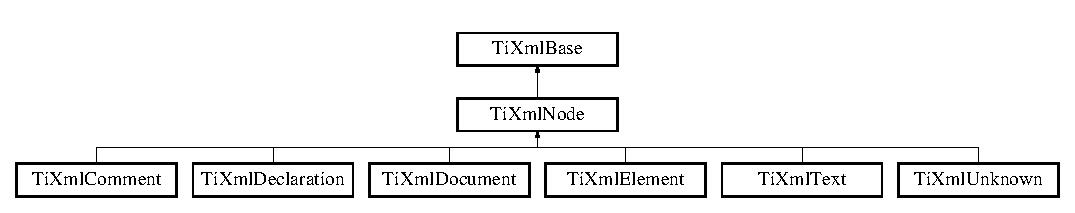
\includegraphics[height=2.413793cm]{class_ti_xml_node}
\end{center}
\end{figure}
\subsection*{Public Types}
\begin{DoxyCompactItemize}
\item 
enum \hyperlink{class_ti_xml_node_a836eded4920ab9e9ef28496f48cd95a2}{Node\+Type} \{ \newline
{\bfseries T\+I\+N\+Y\+X\+M\+L\+\_\+\+D\+O\+C\+U\+M\+E\+NT}, 
{\bfseries T\+I\+N\+Y\+X\+M\+L\+\_\+\+E\+L\+E\+M\+E\+NT}, 
{\bfseries T\+I\+N\+Y\+X\+M\+L\+\_\+\+C\+O\+M\+M\+E\+NT}, 
{\bfseries T\+I\+N\+Y\+X\+M\+L\+\_\+\+U\+N\+K\+N\+O\+WN}, 
\newline
{\bfseries T\+I\+N\+Y\+X\+M\+L\+\_\+\+T\+E\+XT}, 
{\bfseries T\+I\+N\+Y\+X\+M\+L\+\_\+\+D\+E\+C\+L\+A\+R\+A\+T\+I\+ON}, 
{\bfseries T\+I\+N\+Y\+X\+M\+L\+\_\+\+T\+Y\+P\+E\+C\+O\+U\+NT}
 \}
\end{DoxyCompactItemize}
\subsection*{Public Member Functions}
\begin{DoxyCompactItemize}
\item 
const char $\ast$ \hyperlink{class_ti_xml_node_ad44dfe927d49a74dd78b72b7514417ad}{Value} () const
\item 
const std\+::string \& \hyperlink{class_ti_xml_node_a74bda074919e4a5e08d700204793f898}{Value\+Str} () const
\item 
\hypertarget{class_ti_xml_node_a74c4ea4a91c0a91900c919f69f657d6a}{}\label{class_ti_xml_node_a74c4ea4a91c0a91900c919f69f657d6a} 
const T\+I\+X\+M\+L\+\_\+\+S\+T\+R\+I\+NG \& {\bfseries Value\+T\+Str} () const
\item 
void \hyperlink{class_ti_xml_node_a2a38329ca5d3f28f98ce932b8299ae90}{Set\+Value} (const char $\ast$\+\_\+value)
\item 
\hypertarget{class_ti_xml_node_a2598d5f448042c1abbeae4503dd45ff2}{}\label{class_ti_xml_node_a2598d5f448042c1abbeae4503dd45ff2} 
void \hyperlink{class_ti_xml_node_a2598d5f448042c1abbeae4503dd45ff2}{Set\+Value} (const std\+::string \&\+\_\+value)
\begin{DoxyCompactList}\small\item\em S\+TL std\+::string form. \end{DoxyCompactList}\item 
\hypertarget{class_ti_xml_node_a708e7f953df61d4d2d12f73171550a4b}{}\label{class_ti_xml_node_a708e7f953df61d4d2d12f73171550a4b} 
void \hyperlink{class_ti_xml_node_a708e7f953df61d4d2d12f73171550a4b}{Clear} ()
\begin{DoxyCompactList}\small\item\em Delete all the children of this node. Does not affect \textquotesingle{}this\textquotesingle{}. \end{DoxyCompactList}\item 
\hypertarget{class_ti_xml_node_ab643043132ffd794f8602685d34a982e}{}\label{class_ti_xml_node_ab643043132ffd794f8602685d34a982e} 
\hyperlink{class_ti_xml_node}{Ti\+Xml\+Node} $\ast$ \hyperlink{class_ti_xml_node_ab643043132ffd794f8602685d34a982e}{Parent} ()
\begin{DoxyCompactList}\small\item\em One step up the D\+OM. \end{DoxyCompactList}\item 
\hypertarget{class_ti_xml_node_af13df38878a5798142693d01d6133ba0}{}\label{class_ti_xml_node_af13df38878a5798142693d01d6133ba0} 
const \hyperlink{class_ti_xml_node}{Ti\+Xml\+Node} $\ast$ {\bfseries Parent} () const
\item 
\hypertarget{class_ti_xml_node_aa66bceae19707c90c1db12d7c98894a4}{}\label{class_ti_xml_node_aa66bceae19707c90c1db12d7c98894a4} 
const \hyperlink{class_ti_xml_node}{Ti\+Xml\+Node} $\ast$ \hyperlink{class_ti_xml_node_aa66bceae19707c90c1db12d7c98894a4}{First\+Child} () const
\begin{DoxyCompactList}\small\item\em The first child of this node. Will be null if there are no children. \end{DoxyCompactList}\item 
\hypertarget{class_ti_xml_node_a5e97d69b7c0ebd27fb7286be56559b77}{}\label{class_ti_xml_node_a5e97d69b7c0ebd27fb7286be56559b77} 
\hyperlink{class_ti_xml_node}{Ti\+Xml\+Node} $\ast$ {\bfseries First\+Child} ()
\item 
const \hyperlink{class_ti_xml_node}{Ti\+Xml\+Node} $\ast$ \hyperlink{class_ti_xml_node_ae98c367f664890c4b5a5183481ec128a}{First\+Child} (const char $\ast$value) const
\item 
\hypertarget{class_ti_xml_node_abc8bf32be6419ec453a731868de19554}{}\label{class_ti_xml_node_abc8bf32be6419ec453a731868de19554} 
\hyperlink{class_ti_xml_node}{Ti\+Xml\+Node} $\ast$ \hyperlink{class_ti_xml_node_abc8bf32be6419ec453a731868de19554}{First\+Child} (const char $\ast$\+\_\+value)
\begin{DoxyCompactList}\small\item\em The first child of this node with the matching \textquotesingle{}value\textquotesingle{}. Will be null if none found. \end{DoxyCompactList}\item 
\hypertarget{class_ti_xml_node_af3a04120b1ed2fead2f4bb72cbea845e}{}\label{class_ti_xml_node_af3a04120b1ed2fead2f4bb72cbea845e} 
const \hyperlink{class_ti_xml_node}{Ti\+Xml\+Node} $\ast$ {\bfseries Last\+Child} () const
\item 
\hypertarget{class_ti_xml_node_a6432d2b2495f6caf9cb4278df706a031}{}\label{class_ti_xml_node_a6432d2b2495f6caf9cb4278df706a031} 
\hyperlink{class_ti_xml_node}{Ti\+Xml\+Node} $\ast$ \hyperlink{class_ti_xml_node_a6432d2b2495f6caf9cb4278df706a031}{Last\+Child} ()
\begin{DoxyCompactList}\small\item\em The last child of this node. Will be null if there are no children. \end{DoxyCompactList}\item 
\hypertarget{class_ti_xml_node_afdd7b6ba456fdd570610c1d841f91eb3}{}\label{class_ti_xml_node_afdd7b6ba456fdd570610c1d841f91eb3} 
const \hyperlink{class_ti_xml_node}{Ti\+Xml\+Node} $\ast$ {\bfseries Last\+Child} (const char $\ast$value) const
\item 
\hypertarget{class_ti_xml_node_abad5bf1059c48127b958711ef89e8e5d}{}\label{class_ti_xml_node_abad5bf1059c48127b958711ef89e8e5d} 
\hyperlink{class_ti_xml_node}{Ti\+Xml\+Node} $\ast$ \hyperlink{class_ti_xml_node_abad5bf1059c48127b958711ef89e8e5d}{Last\+Child} (const char $\ast$\+\_\+value)
\begin{DoxyCompactList}\small\item\em The last child of this node matching \textquotesingle{}value\textquotesingle{}. Will be null if there are no children. \end{DoxyCompactList}\item 
\hypertarget{class_ti_xml_node_ab7f52e96c41fca07e81521b5f5ea35b9}{}\label{class_ti_xml_node_ab7f52e96c41fca07e81521b5f5ea35b9} 
const \hyperlink{class_ti_xml_node}{Ti\+Xml\+Node} $\ast$ \hyperlink{class_ti_xml_node_ab7f52e96c41fca07e81521b5f5ea35b9}{First\+Child} (const std\+::string \&\+\_\+value) const
\begin{DoxyCompactList}\small\item\em S\+TL std\+::string form. \end{DoxyCompactList}\item 
\hypertarget{class_ti_xml_node_a10d2669ccb5e29e02fcb0e4408685ef6}{}\label{class_ti_xml_node_a10d2669ccb5e29e02fcb0e4408685ef6} 
\hyperlink{class_ti_xml_node}{Ti\+Xml\+Node} $\ast$ \hyperlink{class_ti_xml_node_a10d2669ccb5e29e02fcb0e4408685ef6}{First\+Child} (const std\+::string \&\+\_\+value)
\begin{DoxyCompactList}\small\item\em S\+TL std\+::string form. \end{DoxyCompactList}\item 
\hypertarget{class_ti_xml_node_a96b721f14d5393dac70a0eff0d08520e}{}\label{class_ti_xml_node_a96b721f14d5393dac70a0eff0d08520e} 
const \hyperlink{class_ti_xml_node}{Ti\+Xml\+Node} $\ast$ \hyperlink{class_ti_xml_node_a96b721f14d5393dac70a0eff0d08520e}{Last\+Child} (const std\+::string \&\+\_\+value) const
\begin{DoxyCompactList}\small\item\em S\+TL std\+::string form. \end{DoxyCompactList}\item 
\hypertarget{class_ti_xml_node_a69772c9202f70553f940b15c06b07be3}{}\label{class_ti_xml_node_a69772c9202f70553f940b15c06b07be3} 
\hyperlink{class_ti_xml_node}{Ti\+Xml\+Node} $\ast$ \hyperlink{class_ti_xml_node_a69772c9202f70553f940b15c06b07be3}{Last\+Child} (const std\+::string \&\+\_\+value)
\begin{DoxyCompactList}\small\item\em S\+TL std\+::string form. \end{DoxyCompactList}\item 
const \hyperlink{class_ti_xml_node}{Ti\+Xml\+Node} $\ast$ \hyperlink{class_ti_xml_node_a67c3a02b797f08d9a31b2553661257e1}{Iterate\+Children} (const \hyperlink{class_ti_xml_node}{Ti\+Xml\+Node} $\ast$previous) const
\item 
\hypertarget{class_ti_xml_node_a2358e747118fdbf0e467b1e4f7d03de1}{}\label{class_ti_xml_node_a2358e747118fdbf0e467b1e4f7d03de1} 
\hyperlink{class_ti_xml_node}{Ti\+Xml\+Node} $\ast$ {\bfseries Iterate\+Children} (const \hyperlink{class_ti_xml_node}{Ti\+Xml\+Node} $\ast$previous)
\item 
\hypertarget{class_ti_xml_node_a74bc68a536c279a42af346cb1454f143}{}\label{class_ti_xml_node_a74bc68a536c279a42af346cb1454f143} 
const \hyperlink{class_ti_xml_node}{Ti\+Xml\+Node} $\ast$ \hyperlink{class_ti_xml_node_a74bc68a536c279a42af346cb1454f143}{Iterate\+Children} (const char $\ast$value, const \hyperlink{class_ti_xml_node}{Ti\+Xml\+Node} $\ast$previous) const
\begin{DoxyCompactList}\small\item\em This flavor of Iterate\+Children searches for children with a particular \textquotesingle{}value\textquotesingle{}. \end{DoxyCompactList}\item 
\hypertarget{class_ti_xml_node_a67ba8275e533e6f76340236c42ea0aea}{}\label{class_ti_xml_node_a67ba8275e533e6f76340236c42ea0aea} 
\hyperlink{class_ti_xml_node}{Ti\+Xml\+Node} $\ast$ {\bfseries Iterate\+Children} (const char $\ast$\+\_\+value, const \hyperlink{class_ti_xml_node}{Ti\+Xml\+Node} $\ast$previous)
\item 
\hypertarget{class_ti_xml_node_a412c25b2b7e6709a4b291b13df0632eb}{}\label{class_ti_xml_node_a412c25b2b7e6709a4b291b13df0632eb} 
const \hyperlink{class_ti_xml_node}{Ti\+Xml\+Node} $\ast$ \hyperlink{class_ti_xml_node_a412c25b2b7e6709a4b291b13df0632eb}{Iterate\+Children} (const std\+::string \&\+\_\+value, const \hyperlink{class_ti_xml_node}{Ti\+Xml\+Node} $\ast$previous) const
\begin{DoxyCompactList}\small\item\em S\+TL std\+::string form. \end{DoxyCompactList}\item 
\hypertarget{class_ti_xml_node_a16e9ad53e2f5445b14bf325c90aa862c}{}\label{class_ti_xml_node_a16e9ad53e2f5445b14bf325c90aa862c} 
\hyperlink{class_ti_xml_node}{Ti\+Xml\+Node} $\ast$ \hyperlink{class_ti_xml_node_a16e9ad53e2f5445b14bf325c90aa862c}{Iterate\+Children} (const std\+::string \&\+\_\+value, const \hyperlink{class_ti_xml_node}{Ti\+Xml\+Node} $\ast$previous)
\begin{DoxyCompactList}\small\item\em S\+TL std\+::string form. \end{DoxyCompactList}\item 
\hyperlink{class_ti_xml_node}{Ti\+Xml\+Node} $\ast$ \hyperlink{class_ti_xml_node_af287a913ce46d8dbf7ef24fec69bbaf0}{Insert\+End\+Child} (const \hyperlink{class_ti_xml_node}{Ti\+Xml\+Node} \&add\+This)
\item 
\hyperlink{class_ti_xml_node}{Ti\+Xml\+Node} $\ast$ \hyperlink{class_ti_xml_node_a1a881212554b759865f6cac79a851d38}{Link\+End\+Child} (\hyperlink{class_ti_xml_node}{Ti\+Xml\+Node} $\ast$add\+This)
\item 
\hyperlink{class_ti_xml_node}{Ti\+Xml\+Node} $\ast$ \hyperlink{class_ti_xml_node_a71e54e393336382bc9875f64aab5cb15}{Insert\+Before\+Child} (\hyperlink{class_ti_xml_node}{Ti\+Xml\+Node} $\ast$before\+This, const \hyperlink{class_ti_xml_node}{Ti\+Xml\+Node} \&add\+This)
\item 
\hyperlink{class_ti_xml_node}{Ti\+Xml\+Node} $\ast$ \hyperlink{class_ti_xml_node_a274db3292218202805c093f66a964cb5}{Insert\+After\+Child} (\hyperlink{class_ti_xml_node}{Ti\+Xml\+Node} $\ast$after\+This, const \hyperlink{class_ti_xml_node}{Ti\+Xml\+Node} \&add\+This)
\item 
\hyperlink{class_ti_xml_node}{Ti\+Xml\+Node} $\ast$ \hyperlink{class_ti_xml_node_a543208c2c801c84a213529541e904b9f}{Replace\+Child} (\hyperlink{class_ti_xml_node}{Ti\+Xml\+Node} $\ast$replace\+This, const \hyperlink{class_ti_xml_node}{Ti\+Xml\+Node} \&with\+This)
\item 
\hypertarget{class_ti_xml_node_ae19d8510efc90596552f4feeac9a8fbf}{}\label{class_ti_xml_node_ae19d8510efc90596552f4feeac9a8fbf} 
bool \hyperlink{class_ti_xml_node_ae19d8510efc90596552f4feeac9a8fbf}{Remove\+Child} (\hyperlink{class_ti_xml_node}{Ti\+Xml\+Node} $\ast$remove\+This)
\begin{DoxyCompactList}\small\item\em Delete a child of this node. \end{DoxyCompactList}\item 
\hypertarget{class_ti_xml_node_a8aacf06b1a577ff0d7cfa502cc76da32}{}\label{class_ti_xml_node_a8aacf06b1a577ff0d7cfa502cc76da32} 
const \hyperlink{class_ti_xml_node}{Ti\+Xml\+Node} $\ast$ \hyperlink{class_ti_xml_node_a8aacf06b1a577ff0d7cfa502cc76da32}{Previous\+Sibling} () const
\begin{DoxyCompactList}\small\item\em Navigate to a sibling node. \end{DoxyCompactList}\item 
\hypertarget{class_ti_xml_node_af8c0642ad6ecc03f62953e68896ed1cc}{}\label{class_ti_xml_node_af8c0642ad6ecc03f62953e68896ed1cc} 
\hyperlink{class_ti_xml_node}{Ti\+Xml\+Node} $\ast$ {\bfseries Previous\+Sibling} ()
\item 
\hypertarget{class_ti_xml_node_ace1b618fe58b2b9305fe89bfbc8dd17b}{}\label{class_ti_xml_node_ace1b618fe58b2b9305fe89bfbc8dd17b} 
const \hyperlink{class_ti_xml_node}{Ti\+Xml\+Node} $\ast$ \hyperlink{class_ti_xml_node_ace1b618fe58b2b9305fe89bfbc8dd17b}{Previous\+Sibling} (const char $\ast$) const
\begin{DoxyCompactList}\small\item\em Navigate to a sibling node. \end{DoxyCompactList}\item 
\hypertarget{class_ti_xml_node_a6c977049207177ef21b51972315c2053}{}\label{class_ti_xml_node_a6c977049207177ef21b51972315c2053} 
\hyperlink{class_ti_xml_node}{Ti\+Xml\+Node} $\ast$ {\bfseries Previous\+Sibling} (const char $\ast$\+\_\+prev)
\item 
\hypertarget{class_ti_xml_node_a64ee1c722b607040cd02bd0fd05eb04a}{}\label{class_ti_xml_node_a64ee1c722b607040cd02bd0fd05eb04a} 
const \hyperlink{class_ti_xml_node}{Ti\+Xml\+Node} $\ast$ \hyperlink{class_ti_xml_node_a64ee1c722b607040cd02bd0fd05eb04a}{Previous\+Sibling} (const std\+::string \&\+\_\+value) const
\begin{DoxyCompactList}\small\item\em S\+TL std\+::string form. \end{DoxyCompactList}\item 
\hypertarget{class_ti_xml_node_acc8a0434c7f401d4a3b6dee77c1a5912}{}\label{class_ti_xml_node_acc8a0434c7f401d4a3b6dee77c1a5912} 
\hyperlink{class_ti_xml_node}{Ti\+Xml\+Node} $\ast$ \hyperlink{class_ti_xml_node_acc8a0434c7f401d4a3b6dee77c1a5912}{Previous\+Sibling} (const std\+::string \&\+\_\+value)
\begin{DoxyCompactList}\small\item\em S\+TL std\+::string form. \end{DoxyCompactList}\item 
\hypertarget{class_ti_xml_node_a5f0bf3809d4a35456d28cc9522c26245}{}\label{class_ti_xml_node_a5f0bf3809d4a35456d28cc9522c26245} 
const \hyperlink{class_ti_xml_node}{Ti\+Xml\+Node} $\ast$ \hyperlink{class_ti_xml_node_a5f0bf3809d4a35456d28cc9522c26245}{Next\+Sibling} (const std\+::string \&\+\_\+value) const
\begin{DoxyCompactList}\small\item\em S\+TL std\+::string form. \end{DoxyCompactList}\item 
\hypertarget{class_ti_xml_node_a1757c1f4d01e8c9596ffdbd561c76aea}{}\label{class_ti_xml_node_a1757c1f4d01e8c9596ffdbd561c76aea} 
\hyperlink{class_ti_xml_node}{Ti\+Xml\+Node} $\ast$ \hyperlink{class_ti_xml_node_a1757c1f4d01e8c9596ffdbd561c76aea}{Next\+Sibling} (const std\+::string \&\+\_\+value)
\begin{DoxyCompactList}\small\item\em S\+TL std\+::string form. \end{DoxyCompactList}\item 
\hypertarget{class_ti_xml_node_ae99c572ac7901a15993ea7a4efaa10e7}{}\label{class_ti_xml_node_ae99c572ac7901a15993ea7a4efaa10e7} 
const \hyperlink{class_ti_xml_node}{Ti\+Xml\+Node} $\ast$ \hyperlink{class_ti_xml_node_ae99c572ac7901a15993ea7a4efaa10e7}{Next\+Sibling} () const
\begin{DoxyCompactList}\small\item\em Navigate to a sibling node. \end{DoxyCompactList}\item 
\hypertarget{class_ti_xml_node_a4d05f7b1d7b470ac6887edd072d4892a}{}\label{class_ti_xml_node_a4d05f7b1d7b470ac6887edd072d4892a} 
\hyperlink{class_ti_xml_node}{Ti\+Xml\+Node} $\ast$ {\bfseries Next\+Sibling} ()
\item 
\hypertarget{class_ti_xml_node_a0864ea784b53cdca0a37829d3391ca4b}{}\label{class_ti_xml_node_a0864ea784b53cdca0a37829d3391ca4b} 
const \hyperlink{class_ti_xml_node}{Ti\+Xml\+Node} $\ast$ \hyperlink{class_ti_xml_node_a0864ea784b53cdca0a37829d3391ca4b}{Next\+Sibling} (const char $\ast$) const
\begin{DoxyCompactList}\small\item\em Navigate to a sibling node with the given \textquotesingle{}value\textquotesingle{}. \end{DoxyCompactList}\item 
\hypertarget{class_ti_xml_node_a4080bc5cc8a5c139e7cf308669e850fc}{}\label{class_ti_xml_node_a4080bc5cc8a5c139e7cf308669e850fc} 
\hyperlink{class_ti_xml_node}{Ti\+Xml\+Node} $\ast$ {\bfseries Next\+Sibling} (const char $\ast$\+\_\+next)
\item 
const \hyperlink{class_ti_xml_element}{Ti\+Xml\+Element} $\ast$ \hyperlink{class_ti_xml_node_ac6105781c913a42aa7f3f17bd1964f7c}{Next\+Sibling\+Element} () const
\item 
\hypertarget{class_ti_xml_node_a1b211cb5034655a04358e0e2f6fc5010}{}\label{class_ti_xml_node_a1b211cb5034655a04358e0e2f6fc5010} 
\hyperlink{class_ti_xml_element}{Ti\+Xml\+Element} $\ast$ {\bfseries Next\+Sibling\+Element} ()
\item 
const \hyperlink{class_ti_xml_element}{Ti\+Xml\+Element} $\ast$ \hyperlink{class_ti_xml_node_a22def4746238abaee042f99b47ef3c94}{Next\+Sibling\+Element} (const char $\ast$) const
\item 
\hypertarget{class_ti_xml_node_a6e1ac6b800e18049bc75e9f8e63a8e5f}{}\label{class_ti_xml_node_a6e1ac6b800e18049bc75e9f8e63a8e5f} 
\hyperlink{class_ti_xml_element}{Ti\+Xml\+Element} $\ast$ {\bfseries Next\+Sibling\+Element} (const char $\ast$\+\_\+next)
\item 
\hypertarget{class_ti_xml_node_a2dd7a81689a717fe5d15b3520879ff00}{}\label{class_ti_xml_node_a2dd7a81689a717fe5d15b3520879ff00} 
const \hyperlink{class_ti_xml_element}{Ti\+Xml\+Element} $\ast$ \hyperlink{class_ti_xml_node_a2dd7a81689a717fe5d15b3520879ff00}{Next\+Sibling\+Element} (const std\+::string \&\+\_\+value) const
\begin{DoxyCompactList}\small\item\em S\+TL std\+::string form. \end{DoxyCompactList}\item 
\hypertarget{class_ti_xml_node_a506958e34406729a4e4c5326ea39d081}{}\label{class_ti_xml_node_a506958e34406729a4e4c5326ea39d081} 
\hyperlink{class_ti_xml_element}{Ti\+Xml\+Element} $\ast$ \hyperlink{class_ti_xml_node_a506958e34406729a4e4c5326ea39d081}{Next\+Sibling\+Element} (const std\+::string \&\+\_\+value)
\begin{DoxyCompactList}\small\item\em S\+TL std\+::string form. \end{DoxyCompactList}\item 
\hypertarget{class_ti_xml_node_a12c973e1da9e90a178924b8ea5a5f4d1}{}\label{class_ti_xml_node_a12c973e1da9e90a178924b8ea5a5f4d1} 
const \hyperlink{class_ti_xml_element}{Ti\+Xml\+Element} $\ast$ \hyperlink{class_ti_xml_node_a12c973e1da9e90a178924b8ea5a5f4d1}{First\+Child\+Element} () const
\begin{DoxyCompactList}\small\item\em Convenience function to get through elements. \end{DoxyCompactList}\item 
\hypertarget{class_ti_xml_node_aa0fecff1f3866ab33a8a25506e95db1d}{}\label{class_ti_xml_node_aa0fecff1f3866ab33a8a25506e95db1d} 
\hyperlink{class_ti_xml_element}{Ti\+Xml\+Element} $\ast$ {\bfseries First\+Child\+Element} ()
\item 
\hypertarget{class_ti_xml_node_aab23fca4c2455c1d926c35d85a663842}{}\label{class_ti_xml_node_aab23fca4c2455c1d926c35d85a663842} 
const \hyperlink{class_ti_xml_element}{Ti\+Xml\+Element} $\ast$ \hyperlink{class_ti_xml_node_aab23fca4c2455c1d926c35d85a663842}{First\+Child\+Element} (const char $\ast$\+\_\+value) const
\begin{DoxyCompactList}\small\item\em Convenience function to get through elements. \end{DoxyCompactList}\item 
\hypertarget{class_ti_xml_node_a6936ae323675071808ac4840379e57f5}{}\label{class_ti_xml_node_a6936ae323675071808ac4840379e57f5} 
\hyperlink{class_ti_xml_element}{Ti\+Xml\+Element} $\ast$ {\bfseries First\+Child\+Element} (const char $\ast$\+\_\+value)
\item 
\hypertarget{class_ti_xml_node_abfe4a2abe61324def87fe421946f9df9}{}\label{class_ti_xml_node_abfe4a2abe61324def87fe421946f9df9} 
const \hyperlink{class_ti_xml_element}{Ti\+Xml\+Element} $\ast$ \hyperlink{class_ti_xml_node_abfe4a2abe61324def87fe421946f9df9}{First\+Child\+Element} (const std\+::string \&\+\_\+value) const
\begin{DoxyCompactList}\small\item\em S\+TL std\+::string form. \end{DoxyCompactList}\item 
\hypertarget{class_ti_xml_node_a7f1d7291880534c1e5cdeb392d8c1f45}{}\label{class_ti_xml_node_a7f1d7291880534c1e5cdeb392d8c1f45} 
\hyperlink{class_ti_xml_element}{Ti\+Xml\+Element} $\ast$ \hyperlink{class_ti_xml_node_a7f1d7291880534c1e5cdeb392d8c1f45}{First\+Child\+Element} (const std\+::string \&\+\_\+value)
\begin{DoxyCompactList}\small\item\em S\+TL std\+::string form. \end{DoxyCompactList}\item 
int \hyperlink{class_ti_xml_node_a0f4dd916b2afc2ab2f1a84f3e2b8fd5d}{Type} () const
\item 
const \hyperlink{class_ti_xml_document}{Ti\+Xml\+Document} $\ast$ \hyperlink{class_ti_xml_node_adcb070acefcbaedaa0673d82e530538b}{Get\+Document} () const
\item 
\hypertarget{class_ti_xml_node_a7b2372c0e7adfb32f5b6902fe49a39b2}{}\label{class_ti_xml_node_a7b2372c0e7adfb32f5b6902fe49a39b2} 
\hyperlink{class_ti_xml_document}{Ti\+Xml\+Document} $\ast$ {\bfseries Get\+Document} ()
\item 
\hypertarget{class_ti_xml_node_abe85e0ec04ea59c033f324c8504653e5}{}\label{class_ti_xml_node_abe85e0ec04ea59c033f324c8504653e5} 
bool \hyperlink{class_ti_xml_node_abe85e0ec04ea59c033f324c8504653e5}{No\+Children} () const
\begin{DoxyCompactList}\small\item\em Returns true if this node has no children. \end{DoxyCompactList}\item 
\hypertarget{class_ti_xml_node_a775a904618cad6e4a8049bda4f5a6aa9}{}\label{class_ti_xml_node_a775a904618cad6e4a8049bda4f5a6aa9} 
virtual const \hyperlink{class_ti_xml_document}{Ti\+Xml\+Document} $\ast$ \hyperlink{class_ti_xml_node_a775a904618cad6e4a8049bda4f5a6aa9}{To\+Document} () const
\begin{DoxyCompactList}\small\item\em Cast to a more defined type. Will return null if not of the requested type. \end{DoxyCompactList}\item 
\hypertarget{class_ti_xml_node_a4080428f2cac46e92ef4d284202fad0b}{}\label{class_ti_xml_node_a4080428f2cac46e92ef4d284202fad0b} 
virtual const \hyperlink{class_ti_xml_element}{Ti\+Xml\+Element} $\ast$ \hyperlink{class_ti_xml_node_a4080428f2cac46e92ef4d284202fad0b}{To\+Element} () const
\begin{DoxyCompactList}\small\item\em Cast to a more defined type. Will return null if not of the requested type. \end{DoxyCompactList}\item 
\hypertarget{class_ti_xml_node_a5ad43b9d545315e9bb4f50d4cb70de9e}{}\label{class_ti_xml_node_a5ad43b9d545315e9bb4f50d4cb70de9e} 
virtual const \hyperlink{class_ti_xml_comment}{Ti\+Xml\+Comment} $\ast$ \hyperlink{class_ti_xml_node_a5ad43b9d545315e9bb4f50d4cb70de9e}{To\+Comment} () const
\begin{DoxyCompactList}\small\item\em Cast to a more defined type. Will return null if not of the requested type. \end{DoxyCompactList}\item 
\hypertarget{class_ti_xml_node_ab4f2e6ce87d36c1b9b7de2529128a460}{}\label{class_ti_xml_node_ab4f2e6ce87d36c1b9b7de2529128a460} 
virtual const \hyperlink{class_ti_xml_unknown}{Ti\+Xml\+Unknown} $\ast$ \hyperlink{class_ti_xml_node_ab4f2e6ce87d36c1b9b7de2529128a460}{To\+Unknown} () const
\begin{DoxyCompactList}\small\item\em Cast to a more defined type. Will return null if not of the requested type. \end{DoxyCompactList}\item 
\hypertarget{class_ti_xml_node_a2591700660b308571c09166559a39332}{}\label{class_ti_xml_node_a2591700660b308571c09166559a39332} 
virtual const \hyperlink{class_ti_xml_text}{Ti\+Xml\+Text} $\ast$ \hyperlink{class_ti_xml_node_a2591700660b308571c09166559a39332}{To\+Text} () const
\begin{DoxyCompactList}\small\item\em Cast to a more defined type. Will return null if not of the requested type. \end{DoxyCompactList}\item 
\hypertarget{class_ti_xml_node_a0dc0831e89d499ca911a3be61a413d45}{}\label{class_ti_xml_node_a0dc0831e89d499ca911a3be61a413d45} 
virtual const \hyperlink{class_ti_xml_declaration}{Ti\+Xml\+Declaration} $\ast$ \hyperlink{class_ti_xml_node_a0dc0831e89d499ca911a3be61a413d45}{To\+Declaration} () const
\begin{DoxyCompactList}\small\item\em Cast to a more defined type. Will return null if not of the requested type. \end{DoxyCompactList}\item 
\hypertarget{class_ti_xml_node_a6a4c8ac28ee7a745d059db6691e03bae}{}\label{class_ti_xml_node_a6a4c8ac28ee7a745d059db6691e03bae} 
virtual \hyperlink{class_ti_xml_document}{Ti\+Xml\+Document} $\ast$ \hyperlink{class_ti_xml_node_a6a4c8ac28ee7a745d059db6691e03bae}{To\+Document} ()
\begin{DoxyCompactList}\small\item\em Cast to a more defined type. Will return null if not of the requested type. \end{DoxyCompactList}\item 
\hypertarget{class_ti_xml_node_aa65d000223187d22a4dcebd7479e9ebc}{}\label{class_ti_xml_node_aa65d000223187d22a4dcebd7479e9ebc} 
virtual \hyperlink{class_ti_xml_element}{Ti\+Xml\+Element} $\ast$ \hyperlink{class_ti_xml_node_aa65d000223187d22a4dcebd7479e9ebc}{To\+Element} ()
\begin{DoxyCompactList}\small\item\em Cast to a more defined type. Will return null if not of the requested type. \end{DoxyCompactList}\item 
\hypertarget{class_ti_xml_node_a383e06a0787f7063953934867990f849}{}\label{class_ti_xml_node_a383e06a0787f7063953934867990f849} 
virtual \hyperlink{class_ti_xml_comment}{Ti\+Xml\+Comment} $\ast$ \hyperlink{class_ti_xml_node_a383e06a0787f7063953934867990f849}{To\+Comment} ()
\begin{DoxyCompactList}\small\item\em Cast to a more defined type. Will return null if not of the requested type. \end{DoxyCompactList}\item 
\hypertarget{class_ti_xml_node_a06de5af852668c7e4af0d09c205f0b0d}{}\label{class_ti_xml_node_a06de5af852668c7e4af0d09c205f0b0d} 
virtual \hyperlink{class_ti_xml_unknown}{Ti\+Xml\+Unknown} $\ast$ \hyperlink{class_ti_xml_node_a06de5af852668c7e4af0d09c205f0b0d}{To\+Unknown} ()
\begin{DoxyCompactList}\small\item\em Cast to a more defined type. Will return null if not of the requested type. \end{DoxyCompactList}\item 
\hypertarget{class_ti_xml_node_a3ddfbcac78fbea041fad57e5c6d60a03}{}\label{class_ti_xml_node_a3ddfbcac78fbea041fad57e5c6d60a03} 
virtual \hyperlink{class_ti_xml_text}{Ti\+Xml\+Text} $\ast$ \hyperlink{class_ti_xml_node_a3ddfbcac78fbea041fad57e5c6d60a03}{To\+Text} ()
\begin{DoxyCompactList}\small\item\em Cast to a more defined type. Will return null if not of the requested type. \end{DoxyCompactList}\item 
\hypertarget{class_ti_xml_node_a4027136ca820ff4a636b607231b6a6df}{}\label{class_ti_xml_node_a4027136ca820ff4a636b607231b6a6df} 
virtual \hyperlink{class_ti_xml_declaration}{Ti\+Xml\+Declaration} $\ast$ \hyperlink{class_ti_xml_node_a4027136ca820ff4a636b607231b6a6df}{To\+Declaration} ()
\begin{DoxyCompactList}\small\item\em Cast to a more defined type. Will return null if not of the requested type. \end{DoxyCompactList}\item 
virtual \hyperlink{class_ti_xml_node}{Ti\+Xml\+Node} $\ast$ \hyperlink{class_ti_xml_node_a4508cc3a2d7a98e96a54cc09c37a78a4}{Clone} () const =0
\item 
virtual bool \hyperlink{class_ti_xml_node_acc0f88b7462c6cb73809d410a4f5bb86}{Accept} (\hyperlink{class_ti_xml_visitor}{Ti\+Xml\+Visitor} $\ast$visitor) const =0
\end{DoxyCompactItemize}
\subsection*{Protected Member Functions}
\begin{DoxyCompactItemize}
\item 
\hypertarget{class_ti_xml_node_a3f46721695868667113c7487ff123f20}{}\label{class_ti_xml_node_a3f46721695868667113c7487ff123f20} 
{\bfseries Ti\+Xml\+Node} (\hyperlink{class_ti_xml_node_a836eded4920ab9e9ef28496f48cd95a2}{Node\+Type} \+\_\+type)
\item 
\hypertarget{class_ti_xml_node_aaadd5bb9c94f84c4472b649b95de4a0b}{}\label{class_ti_xml_node_aaadd5bb9c94f84c4472b649b95de4a0b} 
void {\bfseries Copy\+To} (\hyperlink{class_ti_xml_node}{Ti\+Xml\+Node} $\ast$target) const
\item 
\hypertarget{class_ti_xml_node_ab4b4af1a6b486dcbc0e327cf291270af}{}\label{class_ti_xml_node_ab4b4af1a6b486dcbc0e327cf291270af} 
virtual void {\bfseries Stream\+In} (std\+::istream $\ast$in, T\+I\+X\+M\+L\+\_\+\+S\+T\+R\+I\+NG $\ast$tag)=0
\item 
\hypertarget{class_ti_xml_node_ac1e3a8e7578be463b04617786120c2bb}{}\label{class_ti_xml_node_ac1e3a8e7578be463b04617786120c2bb} 
\hyperlink{class_ti_xml_node}{Ti\+Xml\+Node} $\ast$ {\bfseries Identify} (const char $\ast$start, Ti\+Xml\+Encoding encoding)
\end{DoxyCompactItemize}
\subsection*{Protected Attributes}
\begin{DoxyCompactItemize}
\item 
\hypertarget{class_ti_xml_node_a662c4de61244e4fa5bd4e2d8c63143a5}{}\label{class_ti_xml_node_a662c4de61244e4fa5bd4e2d8c63143a5} 
\hyperlink{class_ti_xml_node}{Ti\+Xml\+Node} $\ast$ {\bfseries parent}
\item 
\hypertarget{class_ti_xml_node_a2619c6379181c16ba95ae6922e2ca839}{}\label{class_ti_xml_node_a2619c6379181c16ba95ae6922e2ca839} 
\hyperlink{class_ti_xml_node_a836eded4920ab9e9ef28496f48cd95a2}{Node\+Type} {\bfseries type}
\item 
\hypertarget{class_ti_xml_node_af749fb7f22010b80e8f904c32653d50e}{}\label{class_ti_xml_node_af749fb7f22010b80e8f904c32653d50e} 
\hyperlink{class_ti_xml_node}{Ti\+Xml\+Node} $\ast$ {\bfseries first\+Child}
\item 
\hypertarget{class_ti_xml_node_a5b30756d21b304580d22a841ec9d61f8}{}\label{class_ti_xml_node_a5b30756d21b304580d22a841ec9d61f8} 
\hyperlink{class_ti_xml_node}{Ti\+Xml\+Node} $\ast$ {\bfseries last\+Child}
\item 
\hypertarget{class_ti_xml_node_aead528b3cedc33c16a6c539872c7cc8b}{}\label{class_ti_xml_node_aead528b3cedc33c16a6c539872c7cc8b} 
T\+I\+X\+M\+L\+\_\+\+S\+T\+R\+I\+NG {\bfseries value}
\item 
\hypertarget{class_ti_xml_node_a9c5370ea2cbfd9f0e0f7b30a57fd68f5}{}\label{class_ti_xml_node_a9c5370ea2cbfd9f0e0f7b30a57fd68f5} 
\hyperlink{class_ti_xml_node}{Ti\+Xml\+Node} $\ast$ {\bfseries prev}
\item 
\hypertarget{class_ti_xml_node_a2f329cc993d2d34df76e17dcbb776b45}{}\label{class_ti_xml_node_a2f329cc993d2d34df76e17dcbb776b45} 
\hyperlink{class_ti_xml_node}{Ti\+Xml\+Node} $\ast$ {\bfseries next}
\end{DoxyCompactItemize}
\subsection*{Friends}
\begin{DoxyCompactItemize}
\item 
\hypertarget{class_ti_xml_node_a173617f6dfe902cf484ce5552b950475}{}\label{class_ti_xml_node_a173617f6dfe902cf484ce5552b950475} 
class {\bfseries Ti\+Xml\+Document}
\item 
\hypertarget{class_ti_xml_node_ab6592e32cb9132be517cc12a70564c4b}{}\label{class_ti_xml_node_ab6592e32cb9132be517cc12a70564c4b} 
class {\bfseries Ti\+Xml\+Element}
\item 
std\+::istream \& \hyperlink{class_ti_xml_node_ab57bd426563c926844f65a78412e18b9}{operator$>$$>$} (std\+::istream \&in, \hyperlink{class_ti_xml_node}{Ti\+Xml\+Node} \&base)
\item 
std\+::ostream \& \hyperlink{class_ti_xml_node_a86cd49cfb17a844c0010b3136ac966c7}{operator$<$$<$} (std\+::ostream \&out, const \hyperlink{class_ti_xml_node}{Ti\+Xml\+Node} \&base)
\item 
\hypertarget{class_ti_xml_node_a52ef17e7080df2490cf87bde380685ab}{}\label{class_ti_xml_node_a52ef17e7080df2490cf87bde380685ab} 
std\+::string \& \hyperlink{class_ti_xml_node_a52ef17e7080df2490cf87bde380685ab}{operator$<$$<$} (std\+::string \&out, const \hyperlink{class_ti_xml_node}{Ti\+Xml\+Node} \&base)
\begin{DoxyCompactList}\small\item\em Appends the X\+ML node or attribute to a std\+::string. \end{DoxyCompactList}\end{DoxyCompactItemize}
\subsection*{Additional Inherited Members}


\subsection{Detailed Description}
The parent class for everything in the Document Object \hyperlink{class_model}{Model}. (Except for attributes). Nodes have siblings, a parent, and children. A node can be in a document, or stand on its own. The type of a \hyperlink{class_ti_xml_node}{Ti\+Xml\+Node} can be queried, and it can be cast to its more defined type. 

\subsection{Member Enumeration Documentation}
\hypertarget{class_ti_xml_node_a836eded4920ab9e9ef28496f48cd95a2}{}\label{class_ti_xml_node_a836eded4920ab9e9ef28496f48cd95a2} 
\index{Ti\+Xml\+Node@{Ti\+Xml\+Node}!Node\+Type@{Node\+Type}}
\index{Node\+Type@{Node\+Type}!Ti\+Xml\+Node@{Ti\+Xml\+Node}}
\subsubsection{\texorpdfstring{Node\+Type}{NodeType}}
{\footnotesize\ttfamily enum \hyperlink{class_ti_xml_node_a836eded4920ab9e9ef28496f48cd95a2}{Ti\+Xml\+Node\+::\+Node\+Type}}

The types of X\+ML nodes supported by Tiny\+Xml. (All the unsupported types are picked up by U\+N\+K\+N\+O\+WN.) 

\subsection{Member Function Documentation}
\hypertarget{class_ti_xml_node_acc0f88b7462c6cb73809d410a4f5bb86}{}\label{class_ti_xml_node_acc0f88b7462c6cb73809d410a4f5bb86} 
\index{Ti\+Xml\+Node@{Ti\+Xml\+Node}!Accept@{Accept}}
\index{Accept@{Accept}!Ti\+Xml\+Node@{Ti\+Xml\+Node}}
\subsubsection{\texorpdfstring{Accept()}{Accept()}}
{\footnotesize\ttfamily virtual bool Ti\+Xml\+Node\+::\+Accept (\begin{DoxyParamCaption}\item[{\hyperlink{class_ti_xml_visitor}{Ti\+Xml\+Visitor} $\ast$}]{visitor }\end{DoxyParamCaption}) const\hspace{0.3cm}{\ttfamily [pure virtual]}}

Accept a hierchical visit the nodes in the Tiny\+X\+ML D\+OM. Every node in the X\+ML tree will be conditionally visited and the host will be called back via the \hyperlink{class_ti_xml_visitor}{Ti\+Xml\+Visitor} interface.

This is essentially a S\+AX interface for Tiny\+X\+ML. (Note however it doesn\textquotesingle{}t re-\/parse the X\+ML for the callbacks, so the performance of Tiny\+X\+ML is unchanged by using this interface versus any other.)

The interface has been based on ideas from\+:


\begin{DoxyItemize}
\item \href{http://www.saxproject.org/}{\tt http\+://www.\+saxproject.\+org/}
\item \href{http://c2.com/cgi/wiki?HierarchicalVisitorPattern}{\tt http\+://c2.\+com/cgi/wiki?\+Hierarchical\+Visitor\+Pattern}
\end{DoxyItemize}

Which are both good references for \char`\"{}visiting\char`\"{}.

An example of using \hyperlink{class_ti_xml_node_acc0f88b7462c6cb73809d410a4f5bb86}{Accept()}\+: \begin{DoxyVerb}TiXmlPrinter printer;
tinyxmlDoc.Accept( &printer );
const char* xmlcstr = printer.CStr();
\end{DoxyVerb}
 

Implemented in \hyperlink{class_ti_xml_document_a8ddd6eec722cbd25900bbac664909bac}{Ti\+Xml\+Document}, \hyperlink{class_ti_xml_unknown_aafdf1b2d4f561979c7907bad91004999}{Ti\+Xml\+Unknown}, \hyperlink{class_ti_xml_declaration_aa1b6bade6c989407ce9881bdfc73c1e6}{Ti\+Xml\+Declaration}, \hyperlink{class_ti_xml_text_af65964326eac4640bfb97d4622fa0de2}{Ti\+Xml\+Text}, \hyperlink{class_ti_xml_comment_ac894241530d1d266131a5026cb251a95}{Ti\+Xml\+Comment}, and \hyperlink{class_ti_xml_element_a01d33358cce9d1817b557d314dda3779}{Ti\+Xml\+Element}.

\hypertarget{class_ti_xml_node_a4508cc3a2d7a98e96a54cc09c37a78a4}{}\label{class_ti_xml_node_a4508cc3a2d7a98e96a54cc09c37a78a4} 
\index{Ti\+Xml\+Node@{Ti\+Xml\+Node}!Clone@{Clone}}
\index{Clone@{Clone}!Ti\+Xml\+Node@{Ti\+Xml\+Node}}
\subsubsection{\texorpdfstring{Clone()}{Clone()}}
{\footnotesize\ttfamily virtual \hyperlink{class_ti_xml_node}{Ti\+Xml\+Node}$\ast$ Ti\+Xml\+Node\+::\+Clone (\begin{DoxyParamCaption}{ }\end{DoxyParamCaption}) const\hspace{0.3cm}{\ttfamily [pure virtual]}}

Create an exact duplicate of this node and return it. The memory must be deleted by the caller. 

Implemented in \hyperlink{class_ti_xml_document_a46a4dda6c56eb106d46d4046ae1e5353}{Ti\+Xml\+Document}, \hyperlink{class_ti_xml_unknown_a3dea7689de5b1931fd6657992948fde0}{Ti\+Xml\+Unknown}, \hyperlink{class_ti_xml_declaration_a35dc1455f69b79e81cae28e186944610}{Ti\+Xml\+Declaration}, \hyperlink{class_ti_xml_text_a98a20d7a4f1c1478e25e34921be24bfe}{Ti\+Xml\+Text}, \hyperlink{class_ti_xml_comment_a1f9f06e2ed3f77875093436193b16c16}{Ti\+Xml\+Comment}, and \hyperlink{class_ti_xml_element_a810ea8fa40844c01334e5af2a26794cb}{Ti\+Xml\+Element}.

\hypertarget{class_ti_xml_node_ae98c367f664890c4b5a5183481ec128a}{}\label{class_ti_xml_node_ae98c367f664890c4b5a5183481ec128a} 
\index{Ti\+Xml\+Node@{Ti\+Xml\+Node}!First\+Child@{First\+Child}}
\index{First\+Child@{First\+Child}!Ti\+Xml\+Node@{Ti\+Xml\+Node}}
\subsubsection{\texorpdfstring{First\+Child()}{FirstChild()}}
{\footnotesize\ttfamily const \hyperlink{class_ti_xml_node}{Ti\+Xml\+Node} $\ast$ Ti\+Xml\+Node\+::\+First\+Child (\begin{DoxyParamCaption}\item[{const char $\ast$}]{value }\end{DoxyParamCaption}) const}

The first child of this node with the matching \textquotesingle{}value\textquotesingle{}. Will be null if none found. \hypertarget{class_ti_xml_node_adcb070acefcbaedaa0673d82e530538b}{}\label{class_ti_xml_node_adcb070acefcbaedaa0673d82e530538b} 
\index{Ti\+Xml\+Node@{Ti\+Xml\+Node}!Get\+Document@{Get\+Document}}
\index{Get\+Document@{Get\+Document}!Ti\+Xml\+Node@{Ti\+Xml\+Node}}
\subsubsection{\texorpdfstring{Get\+Document()}{GetDocument()}}
{\footnotesize\ttfamily const \hyperlink{class_ti_xml_document}{Ti\+Xml\+Document} $\ast$ Ti\+Xml\+Node\+::\+Get\+Document (\begin{DoxyParamCaption}{ }\end{DoxyParamCaption}) const}

Return a pointer to the Document this node lives in. Returns null if not in a document. \hypertarget{class_ti_xml_node_a274db3292218202805c093f66a964cb5}{}\label{class_ti_xml_node_a274db3292218202805c093f66a964cb5} 
\index{Ti\+Xml\+Node@{Ti\+Xml\+Node}!Insert\+After\+Child@{Insert\+After\+Child}}
\index{Insert\+After\+Child@{Insert\+After\+Child}!Ti\+Xml\+Node@{Ti\+Xml\+Node}}
\subsubsection{\texorpdfstring{Insert\+After\+Child()}{InsertAfterChild()}}
{\footnotesize\ttfamily \hyperlink{class_ti_xml_node}{Ti\+Xml\+Node} $\ast$ Ti\+Xml\+Node\+::\+Insert\+After\+Child (\begin{DoxyParamCaption}\item[{\hyperlink{class_ti_xml_node}{Ti\+Xml\+Node} $\ast$}]{after\+This,  }\item[{const \hyperlink{class_ti_xml_node}{Ti\+Xml\+Node} \&}]{add\+This }\end{DoxyParamCaption})}

Add a new node related to this. Adds a child after the specified child. Returns a pointer to the new object or N\+U\+LL if an error occured. \hypertarget{class_ti_xml_node_a71e54e393336382bc9875f64aab5cb15}{}\label{class_ti_xml_node_a71e54e393336382bc9875f64aab5cb15} 
\index{Ti\+Xml\+Node@{Ti\+Xml\+Node}!Insert\+Before\+Child@{Insert\+Before\+Child}}
\index{Insert\+Before\+Child@{Insert\+Before\+Child}!Ti\+Xml\+Node@{Ti\+Xml\+Node}}
\subsubsection{\texorpdfstring{Insert\+Before\+Child()}{InsertBeforeChild()}}
{\footnotesize\ttfamily \hyperlink{class_ti_xml_node}{Ti\+Xml\+Node} $\ast$ Ti\+Xml\+Node\+::\+Insert\+Before\+Child (\begin{DoxyParamCaption}\item[{\hyperlink{class_ti_xml_node}{Ti\+Xml\+Node} $\ast$}]{before\+This,  }\item[{const \hyperlink{class_ti_xml_node}{Ti\+Xml\+Node} \&}]{add\+This }\end{DoxyParamCaption})}

Add a new node related to this. Adds a child before the specified child. Returns a pointer to the new object or N\+U\+LL if an error occured. \hypertarget{class_ti_xml_node_af287a913ce46d8dbf7ef24fec69bbaf0}{}\label{class_ti_xml_node_af287a913ce46d8dbf7ef24fec69bbaf0} 
\index{Ti\+Xml\+Node@{Ti\+Xml\+Node}!Insert\+End\+Child@{Insert\+End\+Child}}
\index{Insert\+End\+Child@{Insert\+End\+Child}!Ti\+Xml\+Node@{Ti\+Xml\+Node}}
\subsubsection{\texorpdfstring{Insert\+End\+Child()}{InsertEndChild()}}
{\footnotesize\ttfamily \hyperlink{class_ti_xml_node}{Ti\+Xml\+Node} $\ast$ Ti\+Xml\+Node\+::\+Insert\+End\+Child (\begin{DoxyParamCaption}\item[{const \hyperlink{class_ti_xml_node}{Ti\+Xml\+Node} \&}]{add\+This }\end{DoxyParamCaption})}

Add a new node related to this. Adds a child past the Last\+Child. Returns a pointer to the new object or N\+U\+LL if an error occured. \hypertarget{class_ti_xml_node_a67c3a02b797f08d9a31b2553661257e1}{}\label{class_ti_xml_node_a67c3a02b797f08d9a31b2553661257e1} 
\index{Ti\+Xml\+Node@{Ti\+Xml\+Node}!Iterate\+Children@{Iterate\+Children}}
\index{Iterate\+Children@{Iterate\+Children}!Ti\+Xml\+Node@{Ti\+Xml\+Node}}
\subsubsection{\texorpdfstring{Iterate\+Children()}{IterateChildren()}}
{\footnotesize\ttfamily const \hyperlink{class_ti_xml_node}{Ti\+Xml\+Node} $\ast$ Ti\+Xml\+Node\+::\+Iterate\+Children (\begin{DoxyParamCaption}\item[{const \hyperlink{class_ti_xml_node}{Ti\+Xml\+Node} $\ast$}]{previous }\end{DoxyParamCaption}) const}

An alternate way to walk the children of a node. One way to iterate over nodes is\+: \begin{DoxyVerb}    for( child = parent->FirstChild(); child; child = child->NextSibling() )
\end{DoxyVerb}


Iterate\+Children does the same thing with the syntax\+: \begin{DoxyVerb}    child = 0;
    while( child = parent->IterateChildren( child ) )
\end{DoxyVerb}


Iterate\+Children takes the previous child as input and finds the next one. If the previous child is null, it returns the first. Iterate\+Children will return null when done. \hypertarget{class_ti_xml_node_a1a881212554b759865f6cac79a851d38}{}\label{class_ti_xml_node_a1a881212554b759865f6cac79a851d38} 
\index{Ti\+Xml\+Node@{Ti\+Xml\+Node}!Link\+End\+Child@{Link\+End\+Child}}
\index{Link\+End\+Child@{Link\+End\+Child}!Ti\+Xml\+Node@{Ti\+Xml\+Node}}
\subsubsection{\texorpdfstring{Link\+End\+Child()}{LinkEndChild()}}
{\footnotesize\ttfamily \hyperlink{class_ti_xml_node}{Ti\+Xml\+Node} $\ast$ Ti\+Xml\+Node\+::\+Link\+End\+Child (\begin{DoxyParamCaption}\item[{\hyperlink{class_ti_xml_node}{Ti\+Xml\+Node} $\ast$}]{add\+This }\end{DoxyParamCaption})}

Add a new node related to this. Adds a child past the Last\+Child.

N\+O\+TE\+: the node to be added is passed by pointer, and will be henceforth owned (and deleted) by tiny\+Xml. This method is efficient and avoids an extra copy, but should be used with care as it uses a different memory model than the other insert functions.

\begin{DoxySeeAlso}{See also}
\hyperlink{class_ti_xml_node_af287a913ce46d8dbf7ef24fec69bbaf0}{Insert\+End\+Child} 
\end{DoxySeeAlso}
\hypertarget{class_ti_xml_node_ac6105781c913a42aa7f3f17bd1964f7c}{}\label{class_ti_xml_node_ac6105781c913a42aa7f3f17bd1964f7c} 
\index{Ti\+Xml\+Node@{Ti\+Xml\+Node}!Next\+Sibling\+Element@{Next\+Sibling\+Element}}
\index{Next\+Sibling\+Element@{Next\+Sibling\+Element}!Ti\+Xml\+Node@{Ti\+Xml\+Node}}
\subsubsection{\texorpdfstring{Next\+Sibling\+Element()}{NextSiblingElement()}\hspace{0.1cm}{\footnotesize\ttfamily [1/2]}}
{\footnotesize\ttfamily const \hyperlink{class_ti_xml_element}{Ti\+Xml\+Element} $\ast$ Ti\+Xml\+Node\+::\+Next\+Sibling\+Element (\begin{DoxyParamCaption}{ }\end{DoxyParamCaption}) const}

Convenience function to get through elements. Calls Next\+Sibling and To\+Element. Will skip all non-\/\+Element nodes. Returns 0 if there is not another element. \hypertarget{class_ti_xml_node_a22def4746238abaee042f99b47ef3c94}{}\label{class_ti_xml_node_a22def4746238abaee042f99b47ef3c94} 
\index{Ti\+Xml\+Node@{Ti\+Xml\+Node}!Next\+Sibling\+Element@{Next\+Sibling\+Element}}
\index{Next\+Sibling\+Element@{Next\+Sibling\+Element}!Ti\+Xml\+Node@{Ti\+Xml\+Node}}
\subsubsection{\texorpdfstring{Next\+Sibling\+Element()}{NextSiblingElement()}\hspace{0.1cm}{\footnotesize\ttfamily [2/2]}}
{\footnotesize\ttfamily const \hyperlink{class_ti_xml_element}{Ti\+Xml\+Element} $\ast$ Ti\+Xml\+Node\+::\+Next\+Sibling\+Element (\begin{DoxyParamCaption}\item[{const char $\ast$}]{\+\_\+value }\end{DoxyParamCaption}) const}

Convenience function to get through elements. Calls Next\+Sibling and To\+Element. Will skip all non-\/\+Element nodes. Returns 0 if there is not another element. \hypertarget{class_ti_xml_node_a543208c2c801c84a213529541e904b9f}{}\label{class_ti_xml_node_a543208c2c801c84a213529541e904b9f} 
\index{Ti\+Xml\+Node@{Ti\+Xml\+Node}!Replace\+Child@{Replace\+Child}}
\index{Replace\+Child@{Replace\+Child}!Ti\+Xml\+Node@{Ti\+Xml\+Node}}
\subsubsection{\texorpdfstring{Replace\+Child()}{ReplaceChild()}}
{\footnotesize\ttfamily \hyperlink{class_ti_xml_node}{Ti\+Xml\+Node} $\ast$ Ti\+Xml\+Node\+::\+Replace\+Child (\begin{DoxyParamCaption}\item[{\hyperlink{class_ti_xml_node}{Ti\+Xml\+Node} $\ast$}]{replace\+This,  }\item[{const \hyperlink{class_ti_xml_node}{Ti\+Xml\+Node} \&}]{with\+This }\end{DoxyParamCaption})}

Replace a child of this node. Returns a pointer to the new object or N\+U\+LL if an error occured. \hypertarget{class_ti_xml_node_a2a38329ca5d3f28f98ce932b8299ae90}{}\label{class_ti_xml_node_a2a38329ca5d3f28f98ce932b8299ae90} 
\index{Ti\+Xml\+Node@{Ti\+Xml\+Node}!Set\+Value@{Set\+Value}}
\index{Set\+Value@{Set\+Value}!Ti\+Xml\+Node@{Ti\+Xml\+Node}}
\subsubsection{\texorpdfstring{Set\+Value()}{SetValue()}}
{\footnotesize\ttfamily void Ti\+Xml\+Node\+::\+Set\+Value (\begin{DoxyParamCaption}\item[{const char $\ast$}]{\+\_\+value }\end{DoxyParamCaption})\hspace{0.3cm}{\ttfamily [inline]}}

Changes the value of the node. Defined as\+: \begin{DoxyVerb}Document:   filename of the xml file
Element:    name of the element
Comment:    the comment text
Unknown:    the tag contents
Text:       the text string
\end{DoxyVerb}
 \hypertarget{class_ti_xml_node_a0f4dd916b2afc2ab2f1a84f3e2b8fd5d}{}\label{class_ti_xml_node_a0f4dd916b2afc2ab2f1a84f3e2b8fd5d} 
\index{Ti\+Xml\+Node@{Ti\+Xml\+Node}!Type@{Type}}
\index{Type@{Type}!Ti\+Xml\+Node@{Ti\+Xml\+Node}}
\subsubsection{\texorpdfstring{Type()}{Type()}}
{\footnotesize\ttfamily int Ti\+Xml\+Node\+::\+Type (\begin{DoxyParamCaption}{ }\end{DoxyParamCaption}) const\hspace{0.3cm}{\ttfamily [inline]}}

Query the type (as an enumerated value, above) of this node. The possible types are\+: T\+I\+N\+Y\+X\+M\+L\+\_\+\+D\+O\+C\+U\+M\+E\+NT, T\+I\+N\+Y\+X\+M\+L\+\_\+\+E\+L\+E\+M\+E\+NT, T\+I\+N\+Y\+X\+M\+L\+\_\+\+C\+O\+M\+M\+E\+NT, T\+I\+N\+Y\+X\+M\+L\+\_\+\+U\+N\+K\+N\+O\+WN, T\+I\+N\+Y\+X\+M\+L\+\_\+\+T\+E\+XT, and T\+I\+N\+Y\+X\+M\+L\+\_\+\+D\+E\+C\+L\+A\+R\+A\+T\+I\+ON. \hypertarget{class_ti_xml_node_ad44dfe927d49a74dd78b72b7514417ad}{}\label{class_ti_xml_node_ad44dfe927d49a74dd78b72b7514417ad} 
\index{Ti\+Xml\+Node@{Ti\+Xml\+Node}!Value@{Value}}
\index{Value@{Value}!Ti\+Xml\+Node@{Ti\+Xml\+Node}}
\subsubsection{\texorpdfstring{Value()}{Value()}}
{\footnotesize\ttfamily const char$\ast$ Ti\+Xml\+Node\+::\+Value (\begin{DoxyParamCaption}{ }\end{DoxyParamCaption}) const\hspace{0.3cm}{\ttfamily [inline]}}

The meaning of \textquotesingle{}value\textquotesingle{} changes for the specific type of \hyperlink{class_ti_xml_node}{Ti\+Xml\+Node}. \begin{DoxyVerb}Document:   filename of the xml file
Element:    name of the element
Comment:    the comment text
Unknown:    the tag contents
Text:       the text string
\end{DoxyVerb}


The subclasses will wrap this function. \hypertarget{class_ti_xml_node_a74bda074919e4a5e08d700204793f898}{}\label{class_ti_xml_node_a74bda074919e4a5e08d700204793f898} 
\index{Ti\+Xml\+Node@{Ti\+Xml\+Node}!Value\+Str@{Value\+Str}}
\index{Value\+Str@{Value\+Str}!Ti\+Xml\+Node@{Ti\+Xml\+Node}}
\subsubsection{\texorpdfstring{Value\+Str()}{ValueStr()}}
{\footnotesize\ttfamily const std\+::string\& Ti\+Xml\+Node\+::\+Value\+Str (\begin{DoxyParamCaption}{ }\end{DoxyParamCaption}) const\hspace{0.3cm}{\ttfamily [inline]}}

Return \hyperlink{class_ti_xml_node_ad44dfe927d49a74dd78b72b7514417ad}{Value()} as a std\+::string. If you only use S\+TL, this is more efficient than calling \hyperlink{class_ti_xml_node_ad44dfe927d49a74dd78b72b7514417ad}{Value()}. Only available in S\+TL mode. 

\subsection{Friends And Related Function Documentation}
\hypertarget{class_ti_xml_node_a86cd49cfb17a844c0010b3136ac966c7}{}\label{class_ti_xml_node_a86cd49cfb17a844c0010b3136ac966c7} 
\index{Ti\+Xml\+Node@{Ti\+Xml\+Node}!operator$<$$<$@{operator$<$$<$}}
\index{operator$<$$<$@{operator$<$$<$}!Ti\+Xml\+Node@{Ti\+Xml\+Node}}
\subsubsection{\texorpdfstring{operator$<$$<$}{operator<<}}
{\footnotesize\ttfamily std\+::ostream\& operator$<$$<$ (\begin{DoxyParamCaption}\item[{std\+::ostream \&}]{out,  }\item[{const \hyperlink{class_ti_xml_node}{Ti\+Xml\+Node} \&}]{base }\end{DoxyParamCaption})\hspace{0.3cm}{\ttfamily [friend]}}

An output stream operator, for every class. Note that this outputs without any newlines or formatting, as opposed to \hyperlink{class_ti_xml_base_a0de56b3f2ef14c65091a3b916437b512}{Print()}, which includes tabs and new lines.

The operator$<$$<$ and operator$>$$>$ are not completely symmetric. Writing a node to a stream is very well defined. You\textquotesingle{}ll get a nice stream of output, without any extra whitespace or newlines.

But reading is not as well defined. (As it always is.) If you create a \hyperlink{class_ti_xml_element}{Ti\+Xml\+Element} (for example) and read that from an input stream, the text needs to define an element or junk will result. This is true of all input streams, but it\textquotesingle{}s worth keeping in mind.

A \hyperlink{class_ti_xml_document}{Ti\+Xml\+Document} will read nodes until it reads a root element, and all the children of that root element. \hypertarget{class_ti_xml_node_ab57bd426563c926844f65a78412e18b9}{}\label{class_ti_xml_node_ab57bd426563c926844f65a78412e18b9} 
\index{Ti\+Xml\+Node@{Ti\+Xml\+Node}!operator$>$$>$@{operator$>$$>$}}
\index{operator$>$$>$@{operator$>$$>$}!Ti\+Xml\+Node@{Ti\+Xml\+Node}}
\subsubsection{\texorpdfstring{operator$>$$>$}{operator>>}}
{\footnotesize\ttfamily std\+::istream\& operator$>$$>$ (\begin{DoxyParamCaption}\item[{std\+::istream \&}]{in,  }\item[{\hyperlink{class_ti_xml_node}{Ti\+Xml\+Node} \&}]{base }\end{DoxyParamCaption})\hspace{0.3cm}{\ttfamily [friend]}}

An input stream operator, for every class. Tolerant of newlines and formatting, but doesn\textquotesingle{}t expect them. 

The documentation for this class was generated from the following files\+:\begin{DoxyCompactItemize}
\item 
utility/tiny\+\_\+xml/tinyxml.\+h\item 
utility/tiny\+\_\+xml/tinyxml.\+cpp\item 
utility/tiny\+\_\+xml/tinyxmlparser.\+cpp\end{DoxyCompactItemize}

\hypertarget{class_ti_xml_out_stream}{}\section{Ti\+Xml\+Out\+Stream Class Reference}
\label{class_ti_xml_out_stream}\index{Ti\+Xml\+Out\+Stream@{Ti\+Xml\+Out\+Stream}}
Inheritance diagram for Ti\+Xml\+Out\+Stream\+:\begin{figure}[H]
\begin{center}
\leavevmode
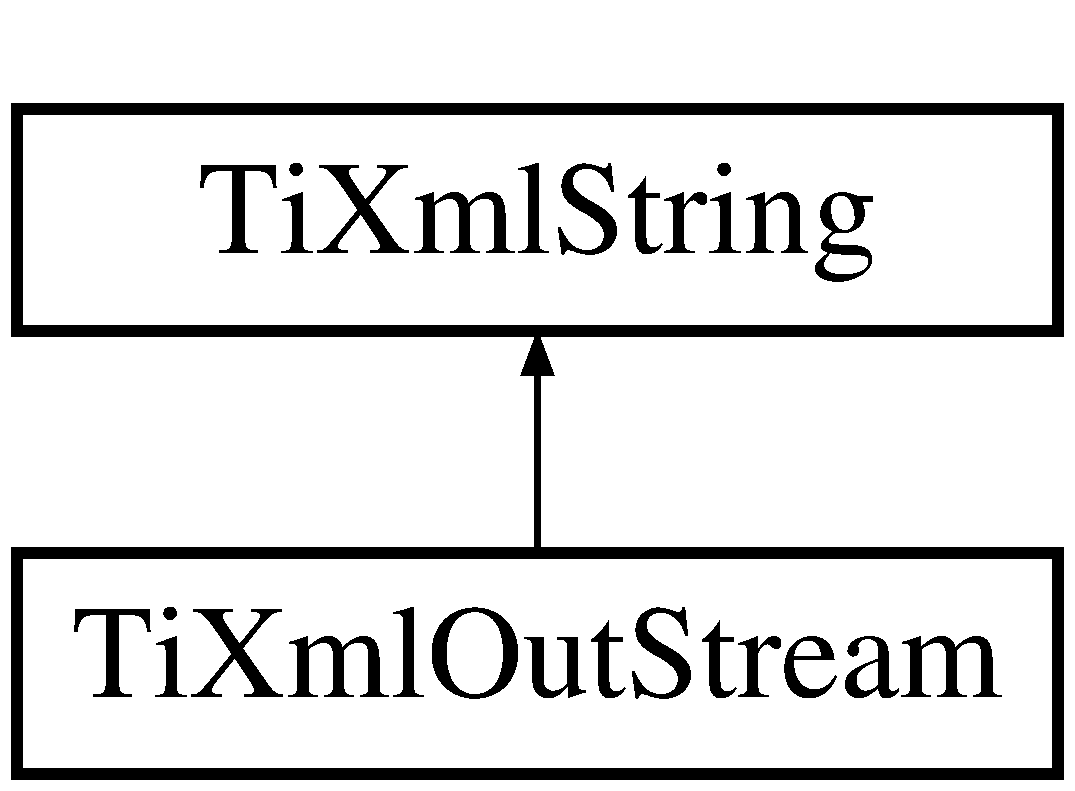
\includegraphics[height=2.000000cm]{class_ti_xml_out_stream}
\end{center}
\end{figure}
\subsection*{Public Member Functions}
\begin{DoxyCompactItemize}
\item 
\hypertarget{class_ti_xml_out_stream_a3640dcb1c0903be3bc6966cdc9a79db6}{}\label{class_ti_xml_out_stream_a3640dcb1c0903be3bc6966cdc9a79db6} 
\hyperlink{class_ti_xml_out_stream}{Ti\+Xml\+Out\+Stream} \& {\bfseries operator$<$$<$} (const \hyperlink{class_ti_xml_string}{Ti\+Xml\+String} \&in)
\item 
\hypertarget{class_ti_xml_out_stream_af2117e5a8cbfcb69544804ad2859bfb6}{}\label{class_ti_xml_out_stream_af2117e5a8cbfcb69544804ad2859bfb6} 
\hyperlink{class_ti_xml_out_stream}{Ti\+Xml\+Out\+Stream} \& {\bfseries operator$<$$<$} (const char $\ast$in)
\end{DoxyCompactItemize}
\subsection*{Additional Inherited Members}


The documentation for this class was generated from the following file\+:\begin{DoxyCompactItemize}
\item 
utility/tiny\+\_\+xml/tinystr.\+h\end{DoxyCompactItemize}

\hypertarget{class_ti_xml_parsing_data}{}\section{Ti\+Xml\+Parsing\+Data Class Reference}
\label{class_ti_xml_parsing_data}\index{Ti\+Xml\+Parsing\+Data@{Ti\+Xml\+Parsing\+Data}}
\subsection*{Public Member Functions}
\begin{DoxyCompactItemize}
\item 
\hypertarget{class_ti_xml_parsing_data_a65cee8ab77a36c605db08c84b4c30a7d}{}\label{class_ti_xml_parsing_data_a65cee8ab77a36c605db08c84b4c30a7d} 
void {\bfseries Stamp} (const char $\ast$now, Ti\+Xml\+Encoding encoding)
\item 
\hypertarget{class_ti_xml_parsing_data_a02ba4903fd3b70b43524ad60a4eece7c}{}\label{class_ti_xml_parsing_data_a02ba4903fd3b70b43524ad60a4eece7c} 
const \hyperlink{struct_ti_xml_cursor}{Ti\+Xml\+Cursor} \& {\bfseries Cursor} () const
\end{DoxyCompactItemize}
\subsection*{Friends}
\begin{DoxyCompactItemize}
\item 
\hypertarget{class_ti_xml_parsing_data_a173617f6dfe902cf484ce5552b950475}{}\label{class_ti_xml_parsing_data_a173617f6dfe902cf484ce5552b950475} 
class {\bfseries Ti\+Xml\+Document}
\end{DoxyCompactItemize}


The documentation for this class was generated from the following file\+:\begin{DoxyCompactItemize}
\item 
utility/tiny\+\_\+xml/tinyxmlparser.\+cpp\end{DoxyCompactItemize}

\hypertarget{class_ti_xml_printer}{}\section{Ti\+Xml\+Printer Class Reference}
\label{class_ti_xml_printer}\index{Ti\+Xml\+Printer@{Ti\+Xml\+Printer}}


{\ttfamily \#include $<$tinyxml.\+h$>$}

Inheritance diagram for Ti\+Xml\+Printer\+:\begin{figure}[H]
\begin{center}
\leavevmode
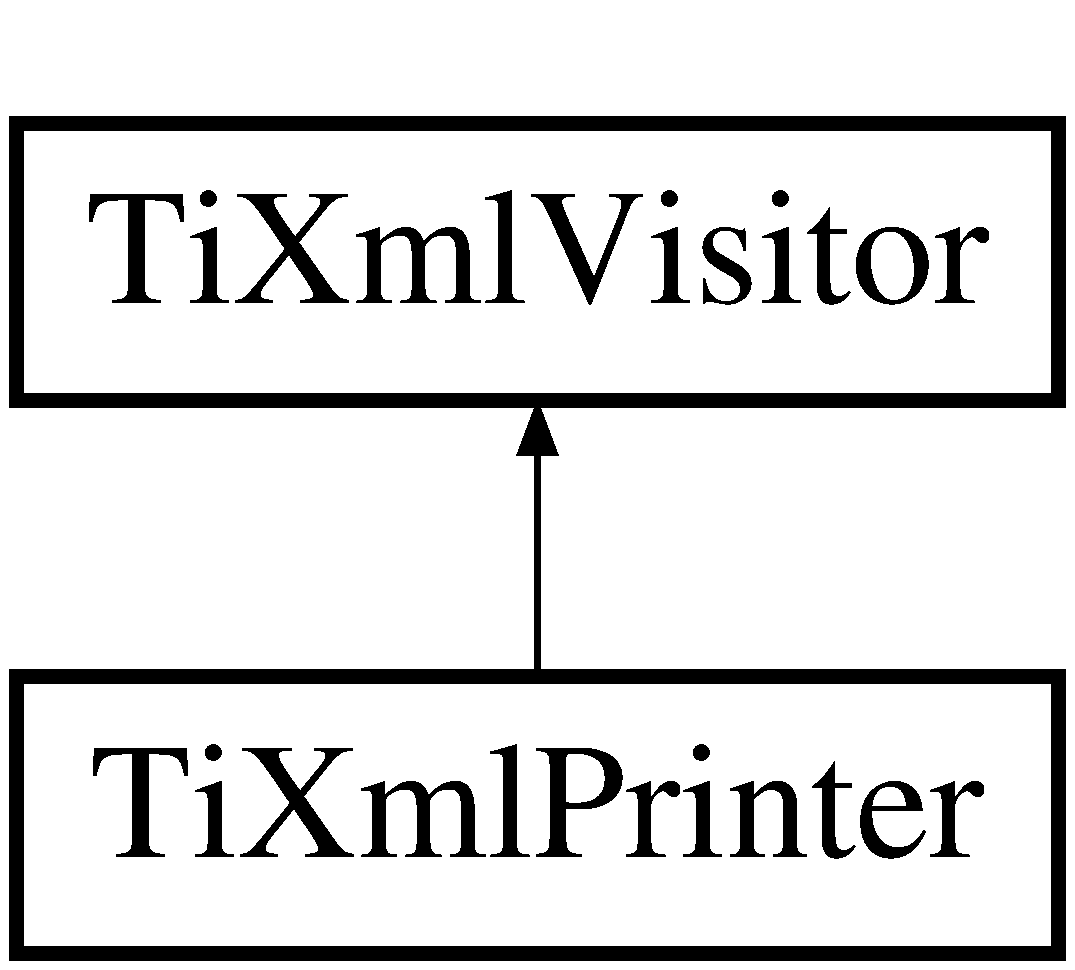
\includegraphics[height=2.000000cm]{class_ti_xml_printer}
\end{center}
\end{figure}
\subsection*{Public Member Functions}
\begin{DoxyCompactItemize}
\item 
\mbox{\Hypertarget{class_ti_xml_printer_a2ec73087db26ff4d2c4316c56f861db7}\label{class_ti_xml_printer_a2ec73087db26ff4d2c4316c56f861db7}} 
virtual bool \hyperlink{class_ti_xml_printer_a2ec73087db26ff4d2c4316c56f861db7}{Visit\+Enter} (const \hyperlink{class_ti_xml_document}{Ti\+Xml\+Document} \&doc)
\begin{DoxyCompactList}\small\item\em Visit a document. \end{DoxyCompactList}\item 
\mbox{\Hypertarget{class_ti_xml_printer_a0a636046fa589b6d7f3e5bd025b3f33e}\label{class_ti_xml_printer_a0a636046fa589b6d7f3e5bd025b3f33e}} 
virtual bool \hyperlink{class_ti_xml_printer_a0a636046fa589b6d7f3e5bd025b3f33e}{Visit\+Exit} (const \hyperlink{class_ti_xml_document}{Ti\+Xml\+Document} \&doc)
\begin{DoxyCompactList}\small\item\em Visit a document. \end{DoxyCompactList}\item 
\mbox{\Hypertarget{class_ti_xml_printer_a6dccaf5ee4979f13877690afe28721e8}\label{class_ti_xml_printer_a6dccaf5ee4979f13877690afe28721e8}} 
virtual bool \hyperlink{class_ti_xml_printer_a6dccaf5ee4979f13877690afe28721e8}{Visit\+Enter} (const \hyperlink{class_ti_xml_element}{Ti\+Xml\+Element} \&element, const \hyperlink{class_ti_xml_attribute}{Ti\+Xml\+Attribute} $\ast$first\+Attribute)
\begin{DoxyCompactList}\small\item\em Visit an element. \end{DoxyCompactList}\item 
\mbox{\Hypertarget{class_ti_xml_printer_ae6a1df8271df4bf62d7873c38e34aa69}\label{class_ti_xml_printer_ae6a1df8271df4bf62d7873c38e34aa69}} 
virtual bool \hyperlink{class_ti_xml_printer_ae6a1df8271df4bf62d7873c38e34aa69}{Visit\+Exit} (const \hyperlink{class_ti_xml_element}{Ti\+Xml\+Element} \&element)
\begin{DoxyCompactList}\small\item\em Visit an element. \end{DoxyCompactList}\item 
\mbox{\Hypertarget{class_ti_xml_printer_adaf7eec4dc43ad071ff52b60361574f5}\label{class_ti_xml_printer_adaf7eec4dc43ad071ff52b60361574f5}} 
virtual bool \hyperlink{class_ti_xml_printer_adaf7eec4dc43ad071ff52b60361574f5}{Visit} (const \hyperlink{class_ti_xml_declaration}{Ti\+Xml\+Declaration} \&declaration)
\begin{DoxyCompactList}\small\item\em Visit a declaration. \end{DoxyCompactList}\item 
\mbox{\Hypertarget{class_ti_xml_printer_a0857c5d32c59b9a257f9a49cb9411df5}\label{class_ti_xml_printer_a0857c5d32c59b9a257f9a49cb9411df5}} 
virtual bool \hyperlink{class_ti_xml_printer_a0857c5d32c59b9a257f9a49cb9411df5}{Visit} (const \hyperlink{class_ti_xml_text}{Ti\+Xml\+Text} \&text)
\begin{DoxyCompactList}\small\item\em Visit a text node. \end{DoxyCompactList}\item 
\mbox{\Hypertarget{class_ti_xml_printer_a9870423f5603630e6142f6bdb66dfb57}\label{class_ti_xml_printer_a9870423f5603630e6142f6bdb66dfb57}} 
virtual bool \hyperlink{class_ti_xml_printer_a9870423f5603630e6142f6bdb66dfb57}{Visit} (const \hyperlink{class_ti_xml_comment}{Ti\+Xml\+Comment} \&comment)
\begin{DoxyCompactList}\small\item\em Visit a comment node. \end{DoxyCompactList}\item 
\mbox{\Hypertarget{class_ti_xml_printer_a08591a15c9a07afa83c24e08b03d6358}\label{class_ti_xml_printer_a08591a15c9a07afa83c24e08b03d6358}} 
virtual bool \hyperlink{class_ti_xml_printer_a08591a15c9a07afa83c24e08b03d6358}{Visit} (const \hyperlink{class_ti_xml_unknown}{Ti\+Xml\+Unknown} \&unknown)
\begin{DoxyCompactList}\small\item\em Visit an unknown node. \end{DoxyCompactList}\item 
void \hyperlink{class_ti_xml_printer_a213377a4070c7e625bae59716b089e5e}{Set\+Indent} (const char $\ast$\+\_\+indent)
\item 
\mbox{\Hypertarget{class_ti_xml_printer_abb33ec7d4bad6aaeb57f4304394b133d}\label{class_ti_xml_printer_abb33ec7d4bad6aaeb57f4304394b133d}} 
const char $\ast$ \hyperlink{class_ti_xml_printer_abb33ec7d4bad6aaeb57f4304394b133d}{Indent} ()
\begin{DoxyCompactList}\small\item\em Query the indention string. \end{DoxyCompactList}\item 
void \hyperlink{class_ti_xml_printer_a4be1e37e69e3858c59635aa947174fe6}{Set\+Line\+Break} (const char $\ast$\+\_\+line\+Break)
\item 
\mbox{\Hypertarget{class_ti_xml_printer_a11f1b4804a460b175ec244eb5724d96d}\label{class_ti_xml_printer_a11f1b4804a460b175ec244eb5724d96d}} 
const char $\ast$ \hyperlink{class_ti_xml_printer_a11f1b4804a460b175ec244eb5724d96d}{Line\+Break} ()
\begin{DoxyCompactList}\small\item\em Query the current line breaking string. \end{DoxyCompactList}\item 
void \hyperlink{class_ti_xml_printer_ab23a90629e374cb1cadca090468bbd19}{Set\+Stream\+Printing} ()
\item 
\mbox{\Hypertarget{class_ti_xml_printer_a859eede9597d3e0355b77757be48735e}\label{class_ti_xml_printer_a859eede9597d3e0355b77757be48735e}} 
const char $\ast$ \hyperlink{class_ti_xml_printer_a859eede9597d3e0355b77757be48735e}{C\+Str} ()
\begin{DoxyCompactList}\small\item\em Return the result. \end{DoxyCompactList}\item 
\mbox{\Hypertarget{class_ti_xml_printer_ad01375ae9199bd2f48252eaddce3039d}\label{class_ti_xml_printer_ad01375ae9199bd2f48252eaddce3039d}} 
size\+\_\+t \hyperlink{class_ti_xml_printer_ad01375ae9199bd2f48252eaddce3039d}{Size} ()
\begin{DoxyCompactList}\small\item\em Return the length of the result string. \end{DoxyCompactList}\item 
\mbox{\Hypertarget{class_ti_xml_printer_a3bd4daf44309b41f5813a833caa0d1c9}\label{class_ti_xml_printer_a3bd4daf44309b41f5813a833caa0d1c9}} 
const std\+::string \& \hyperlink{class_ti_xml_printer_a3bd4daf44309b41f5813a833caa0d1c9}{Str} ()
\begin{DoxyCompactList}\small\item\em Return the result. \end{DoxyCompactList}\end{DoxyCompactItemize}


\subsection{Detailed Description}
Print to memory functionality. The \hyperlink{class_ti_xml_printer}{Ti\+Xml\+Printer} is useful when you need to\+:


\begin{DoxyEnumerate}
\item Print to memory (especially in non-\/\+S\+TL mode)
\item Control formatting (line endings, etc.)
\end{DoxyEnumerate}

When constructed, the \hyperlink{class_ti_xml_printer}{Ti\+Xml\+Printer} is in its default \char`\"{}pretty printing\char`\"{} mode. Before calling Accept() you can call methods to control the printing of the X\+ML document. After \hyperlink{class_ti_xml_node_acc0f88b7462c6cb73809d410a4f5bb86}{Ti\+Xml\+Node\+::\+Accept()} is called, the printed document can be accessed via the \hyperlink{class_ti_xml_printer_a859eede9597d3e0355b77757be48735e}{C\+Str()}, \hyperlink{class_ti_xml_printer_a3bd4daf44309b41f5813a833caa0d1c9}{Str()}, and \hyperlink{class_ti_xml_printer_ad01375ae9199bd2f48252eaddce3039d}{Size()} methods.

\hyperlink{class_ti_xml_printer}{Ti\+Xml\+Printer} uses the Visitor A\+PI. \begin{DoxyVerb}TiXmlPrinter printer;
printer.SetIndent( "\t" );

doc.Accept( &printer );
fprintf( stdout, "%s", printer.CStr() );
\end{DoxyVerb}
 

\subsection{Member Function Documentation}
\mbox{\Hypertarget{class_ti_xml_printer_a213377a4070c7e625bae59716b089e5e}\label{class_ti_xml_printer_a213377a4070c7e625bae59716b089e5e}} 
\index{Ti\+Xml\+Printer@{Ti\+Xml\+Printer}!Set\+Indent@{Set\+Indent}}
\index{Set\+Indent@{Set\+Indent}!Ti\+Xml\+Printer@{Ti\+Xml\+Printer}}
\subsubsection{\texorpdfstring{Set\+Indent()}{SetIndent()}}
{\footnotesize\ttfamily void Ti\+Xml\+Printer\+::\+Set\+Indent (\begin{DoxyParamCaption}\item[{const char $\ast$}]{\+\_\+indent }\end{DoxyParamCaption})\hspace{0.3cm}{\ttfamily [inline]}}

Set the indent characters for printing. By default 4 spaces but tab () is also useful, or null/empty string for no indentation. \mbox{\Hypertarget{class_ti_xml_printer_a4be1e37e69e3858c59635aa947174fe6}\label{class_ti_xml_printer_a4be1e37e69e3858c59635aa947174fe6}} 
\index{Ti\+Xml\+Printer@{Ti\+Xml\+Printer}!Set\+Line\+Break@{Set\+Line\+Break}}
\index{Set\+Line\+Break@{Set\+Line\+Break}!Ti\+Xml\+Printer@{Ti\+Xml\+Printer}}
\subsubsection{\texorpdfstring{Set\+Line\+Break()}{SetLineBreak()}}
{\footnotesize\ttfamily void Ti\+Xml\+Printer\+::\+Set\+Line\+Break (\begin{DoxyParamCaption}\item[{const char $\ast$}]{\+\_\+line\+Break }\end{DoxyParamCaption})\hspace{0.3cm}{\ttfamily [inline]}}

Set the line breaking string. By default set to newline (~\newline
). Some operating systems prefer other characters, or can be set to the null/empty string for no indenation. \mbox{\Hypertarget{class_ti_xml_printer_ab23a90629e374cb1cadca090468bbd19}\label{class_ti_xml_printer_ab23a90629e374cb1cadca090468bbd19}} 
\index{Ti\+Xml\+Printer@{Ti\+Xml\+Printer}!Set\+Stream\+Printing@{Set\+Stream\+Printing}}
\index{Set\+Stream\+Printing@{Set\+Stream\+Printing}!Ti\+Xml\+Printer@{Ti\+Xml\+Printer}}
\subsubsection{\texorpdfstring{Set\+Stream\+Printing()}{SetStreamPrinting()}}
{\footnotesize\ttfamily void Ti\+Xml\+Printer\+::\+Set\+Stream\+Printing (\begin{DoxyParamCaption}{ }\end{DoxyParamCaption})\hspace{0.3cm}{\ttfamily [inline]}}

Switch over to \char`\"{}stream printing\char`\"{} which is the most dense formatting without linebreaks. Common when the X\+ML is needed for network transmission. 

The documentation for this class was generated from the following files\+:\begin{DoxyCompactItemize}
\item 
utility/tiny\+\_\+xml/tinyxml.\+h\item 
utility/tiny\+\_\+xml/tinyxml.\+cpp\end{DoxyCompactItemize}

\hypertarget{class_ti_xml_string}{}\section{Ti\+Xml\+String Class Reference}
\label{class_ti_xml_string}\index{Ti\+Xml\+String@{Ti\+Xml\+String}}
Inheritance diagram for Ti\+Xml\+String\+:\begin{figure}[H]
\begin{center}
\leavevmode
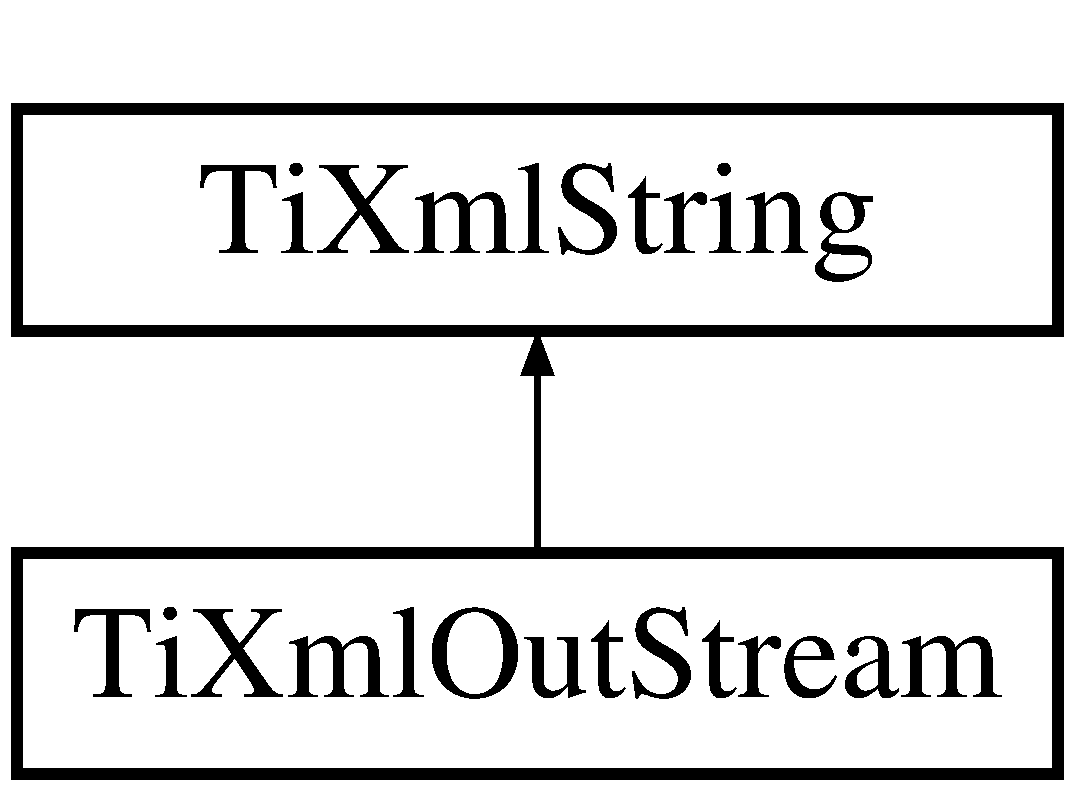
\includegraphics[height=2.000000cm]{class_ti_xml_string}
\end{center}
\end{figure}
\subsection*{Public Types}
\begin{DoxyCompactItemize}
\item 
\mbox{\Hypertarget{class_ti_xml_string_abeb2c1893a04c17904f7c06546d0b971}\label{class_ti_xml_string_abeb2c1893a04c17904f7c06546d0b971}} 
typedef size\+\_\+t {\bfseries size\+\_\+type}
\end{DoxyCompactItemize}
\subsection*{Public Member Functions}
\begin{DoxyCompactItemize}
\item 
\mbox{\Hypertarget{class_ti_xml_string_ac80fe17693a438c9ab2591664743fcb6}\label{class_ti_xml_string_ac80fe17693a438c9ab2591664743fcb6}} 
{\bfseries Ti\+Xml\+String} (const \hyperlink{class_ti_xml_string}{Ti\+Xml\+String} \&copy)
\item 
\mbox{\Hypertarget{class_ti_xml_string_aa3b32bd2891a757c9f36c21db44c81d2}\label{class_ti_xml_string_aa3b32bd2891a757c9f36c21db44c81d2}} 
T\+I\+X\+M\+L\+\_\+\+E\+X\+P\+L\+I\+C\+IT {\bfseries Ti\+Xml\+String} (const char $\ast$copy)
\item 
\mbox{\Hypertarget{class_ti_xml_string_a4b17ea5c5db986f14827223dfa8f1547}\label{class_ti_xml_string_a4b17ea5c5db986f14827223dfa8f1547}} 
T\+I\+X\+M\+L\+\_\+\+E\+X\+P\+L\+I\+C\+IT {\bfseries Ti\+Xml\+String} (const char $\ast$str, size\+\_\+type len)
\item 
\mbox{\Hypertarget{class_ti_xml_string_ae0bc6147afc0ec2aa0da3a3c0a8fcfb0}\label{class_ti_xml_string_ae0bc6147afc0ec2aa0da3a3c0a8fcfb0}} 
\hyperlink{class_ti_xml_string}{Ti\+Xml\+String} \& {\bfseries operator=} (const char $\ast$copy)
\item 
\mbox{\Hypertarget{class_ti_xml_string_ab1f1f5d3eceaa0f22d0a7e6055ea81b0}\label{class_ti_xml_string_ab1f1f5d3eceaa0f22d0a7e6055ea81b0}} 
\hyperlink{class_ti_xml_string}{Ti\+Xml\+String} \& {\bfseries operator=} (const \hyperlink{class_ti_xml_string}{Ti\+Xml\+String} \&copy)
\item 
\mbox{\Hypertarget{class_ti_xml_string_ab56336ac2aa2a08d24a71eb9a2b502a5}\label{class_ti_xml_string_ab56336ac2aa2a08d24a71eb9a2b502a5}} 
\hyperlink{class_ti_xml_string}{Ti\+Xml\+String} \& {\bfseries operator+=} (const char $\ast$suffix)
\item 
\mbox{\Hypertarget{class_ti_xml_string_a6aa09d5240470b76d54ec709e04f8c13}\label{class_ti_xml_string_a6aa09d5240470b76d54ec709e04f8c13}} 
\hyperlink{class_ti_xml_string}{Ti\+Xml\+String} \& {\bfseries operator+=} (char single)
\item 
\mbox{\Hypertarget{class_ti_xml_string_afdcae5ea2b4d9e194dc21226b817f417}\label{class_ti_xml_string_afdcae5ea2b4d9e194dc21226b817f417}} 
\hyperlink{class_ti_xml_string}{Ti\+Xml\+String} \& {\bfseries operator+=} (const \hyperlink{class_ti_xml_string}{Ti\+Xml\+String} \&suffix)
\item 
\mbox{\Hypertarget{class_ti_xml_string_ae2bd36349215612ebcc3cb221c30bd3d}\label{class_ti_xml_string_ae2bd36349215612ebcc3cb221c30bd3d}} 
const char $\ast$ {\bfseries c\+\_\+str} () const
\item 
\mbox{\Hypertarget{class_ti_xml_string_a0e010e1737cfc3ee885b42875171b88e}\label{class_ti_xml_string_a0e010e1737cfc3ee885b42875171b88e}} 
const char $\ast$ {\bfseries data} () const
\item 
\mbox{\Hypertarget{class_ti_xml_string_a5db17f8314ffe2a89df0f0eb6c2a4bf5}\label{class_ti_xml_string_a5db17f8314ffe2a89df0f0eb6c2a4bf5}} 
size\+\_\+type {\bfseries length} () const
\item 
\mbox{\Hypertarget{class_ti_xml_string_a483d85103d2a3ba8c0831e205c832f33}\label{class_ti_xml_string_a483d85103d2a3ba8c0831e205c832f33}} 
size\+\_\+type {\bfseries size} () const
\item 
\mbox{\Hypertarget{class_ti_xml_string_a3139aafb0f0a8e26d1a4ed58a50f3678}\label{class_ti_xml_string_a3139aafb0f0a8e26d1a4ed58a50f3678}} 
bool {\bfseries empty} () const
\item 
\mbox{\Hypertarget{class_ti_xml_string_a0ca248f026e698f79b8aa4c9ab8e1571}\label{class_ti_xml_string_a0ca248f026e698f79b8aa4c9ab8e1571}} 
size\+\_\+type {\bfseries capacity} () const
\item 
\mbox{\Hypertarget{class_ti_xml_string_a7f33c37f7dfde5193f02521d2a7af1db}\label{class_ti_xml_string_a7f33c37f7dfde5193f02521d2a7af1db}} 
const char \& {\bfseries at} (size\+\_\+type index) const
\item 
\mbox{\Hypertarget{class_ti_xml_string_a06e8c84831fc146610369405f4aa4200}\label{class_ti_xml_string_a06e8c84831fc146610369405f4aa4200}} 
char \& {\bfseries operator\mbox{[}$\,$\mbox{]}} (size\+\_\+type index) const
\item 
\mbox{\Hypertarget{class_ti_xml_string_a22fc54a23c5a0ab771331a25a769516e}\label{class_ti_xml_string_a22fc54a23c5a0ab771331a25a769516e}} 
size\+\_\+type {\bfseries find} (char lookup) const
\item 
\mbox{\Hypertarget{class_ti_xml_string_a2d66cfd6986faceda62ca62db553a921}\label{class_ti_xml_string_a2d66cfd6986faceda62ca62db553a921}} 
size\+\_\+type {\bfseries find} (char tofind, size\+\_\+type offset) const
\item 
\mbox{\Hypertarget{class_ti_xml_string_ab20e06e4c666abf3bdbfb3a1191d4888}\label{class_ti_xml_string_ab20e06e4c666abf3bdbfb3a1191d4888}} 
void {\bfseries clear} ()
\item 
\mbox{\Hypertarget{class_ti_xml_string_a88ecf9f0f00cb5c67b6b637958d7049c}\label{class_ti_xml_string_a88ecf9f0f00cb5c67b6b637958d7049c}} 
void {\bfseries reserve} (size\+\_\+type cap)
\item 
\mbox{\Hypertarget{class_ti_xml_string_ac72f3d9149b7812c1e6c59402014d0d5}\label{class_ti_xml_string_ac72f3d9149b7812c1e6c59402014d0d5}} 
\hyperlink{class_ti_xml_string}{Ti\+Xml\+String} \& {\bfseries assign} (const char $\ast$str, size\+\_\+type len)
\item 
\mbox{\Hypertarget{class_ti_xml_string_ad44b21700d2ec24a511367b222b643fb}\label{class_ti_xml_string_ad44b21700d2ec24a511367b222b643fb}} 
\hyperlink{class_ti_xml_string}{Ti\+Xml\+String} \& {\bfseries append} (const char $\ast$str, size\+\_\+type len)
\item 
\mbox{\Hypertarget{class_ti_xml_string_aa392cbc180752a79f007f4f9280c7762}\label{class_ti_xml_string_aa392cbc180752a79f007f4f9280c7762}} 
void {\bfseries swap} (\hyperlink{class_ti_xml_string}{Ti\+Xml\+String} \&other)
\end{DoxyCompactItemize}
\subsection*{Static Public Attributes}
\begin{DoxyCompactItemize}
\item 
\mbox{\Hypertarget{class_ti_xml_string_a8f4422d227088dc7bec96f479b275d0a}\label{class_ti_xml_string_a8f4422d227088dc7bec96f479b275d0a}} 
static const size\+\_\+type {\bfseries npos} = static\+\_\+cast$<$ Ti\+Xml\+String\+::size\+\_\+type $>$(-\/1)
\end{DoxyCompactItemize}


The documentation for this class was generated from the following files\+:\begin{DoxyCompactItemize}
\item 
utility/tiny\+\_\+xml/tinystr.\+h\item 
utility/tiny\+\_\+xml/tinystr.\+cpp\end{DoxyCompactItemize}

\hypertarget{class_ti_xml_text}{}\section{Ti\+Xml\+Text Class Reference}
\label{class_ti_xml_text}\index{Ti\+Xml\+Text@{Ti\+Xml\+Text}}


{\ttfamily \#include $<$tinyxml.\+h$>$}

Inheritance diagram for Ti\+Xml\+Text\+:\begin{figure}[H]
\begin{center}
\leavevmode
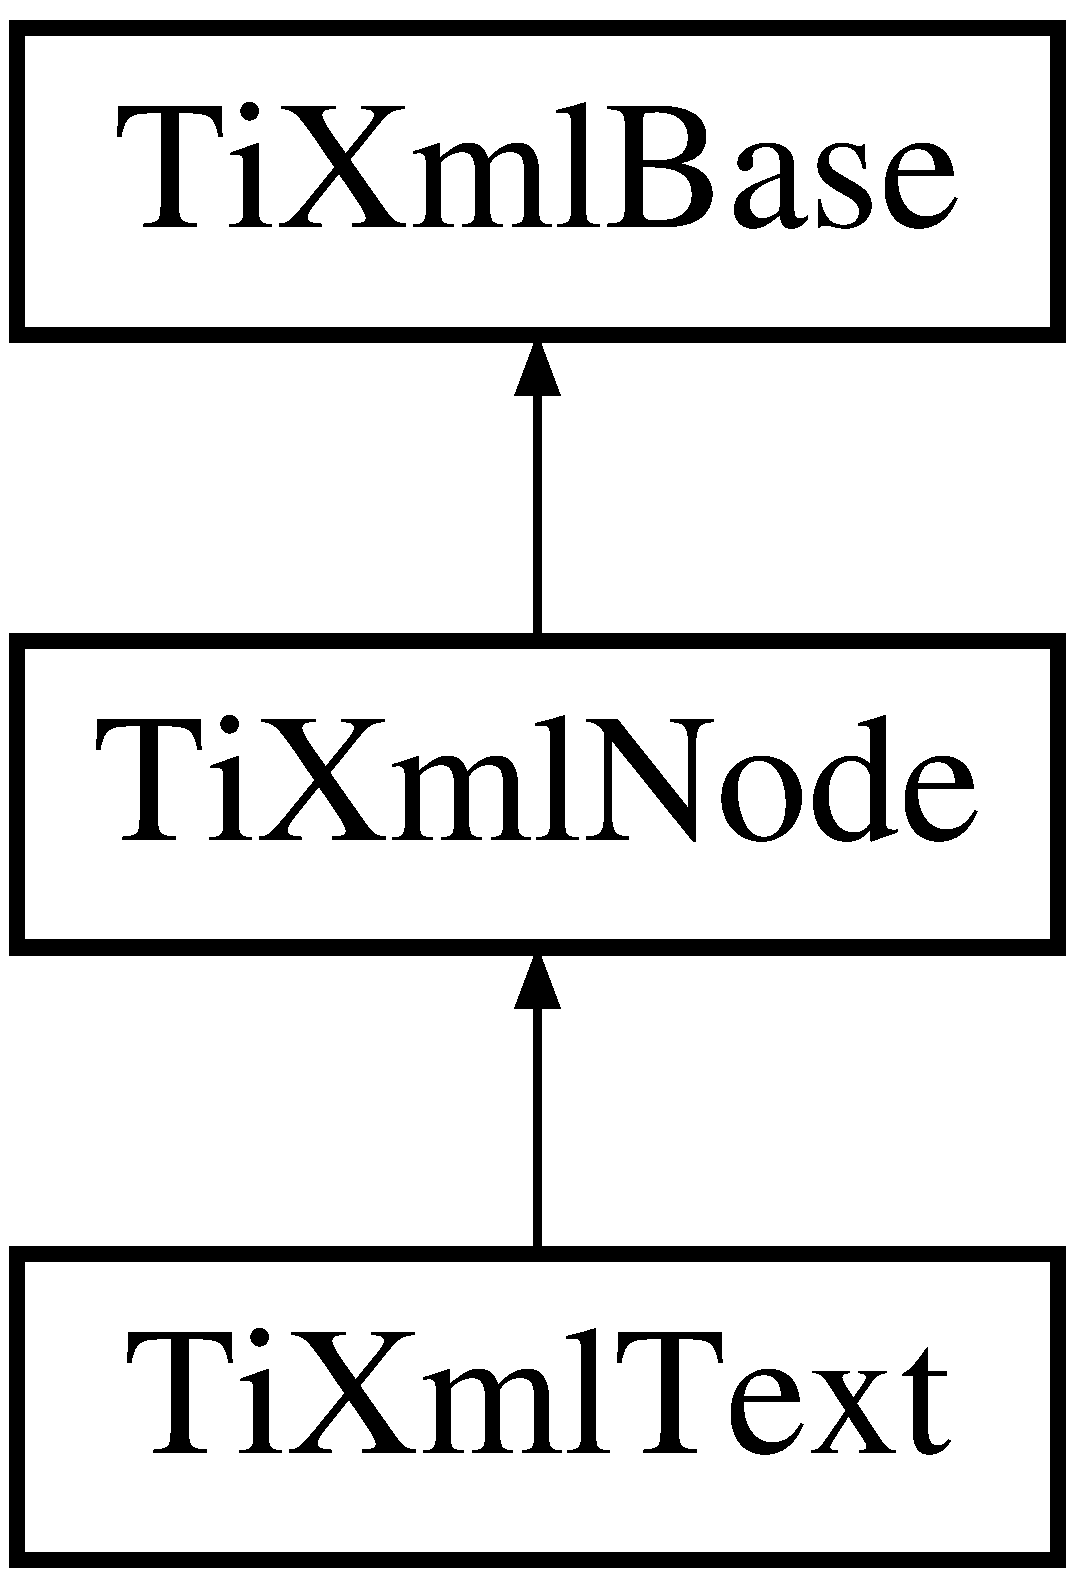
\includegraphics[height=3.000000cm]{class_ti_xml_text}
\end{center}
\end{figure}
\subsection*{Public Member Functions}
\begin{DoxyCompactItemize}
\item 
\hyperlink{class_ti_xml_text_af659e77c6b87d684827f35a8f4895960}{Ti\+Xml\+Text} (const char $\ast$init\+Value)
\item 
\mbox{\Hypertarget{class_ti_xml_text_a439792f6183a3d3fb6f2bc2b16fa5691}\label{class_ti_xml_text_a439792f6183a3d3fb6f2bc2b16fa5691}} 
\hyperlink{class_ti_xml_text_a439792f6183a3d3fb6f2bc2b16fa5691}{Ti\+Xml\+Text} (const std\+::string \&init\+Value)
\begin{DoxyCompactList}\small\item\em Constructor. \end{DoxyCompactList}\item 
\mbox{\Hypertarget{class_ti_xml_text_a8d2cc1b4af2208cbb0171cf20f6815d1}\label{class_ti_xml_text_a8d2cc1b4af2208cbb0171cf20f6815d1}} 
{\bfseries Ti\+Xml\+Text} (const \hyperlink{class_ti_xml_text}{Ti\+Xml\+Text} \&copy)
\item 
\mbox{\Hypertarget{class_ti_xml_text_aed5b13f9c1b804c616fd533882c29f57}\label{class_ti_xml_text_aed5b13f9c1b804c616fd533882c29f57}} 
\hyperlink{class_ti_xml_text}{Ti\+Xml\+Text} \& {\bfseries operator=} (const \hyperlink{class_ti_xml_text}{Ti\+Xml\+Text} \&base)
\item 
virtual void \hyperlink{class_ti_xml_text_a75f6895906333894e2574cc8cf77ea79}{Print} (F\+I\+LE $\ast$cfile, int depth) const
\item 
\mbox{\Hypertarget{class_ti_xml_text_aac1f4764d220ed6bf809b16dfcb6b45a}\label{class_ti_xml_text_aac1f4764d220ed6bf809b16dfcb6b45a}} 
bool \hyperlink{class_ti_xml_text_aac1f4764d220ed6bf809b16dfcb6b45a}{C\+D\+A\+TA} () const
\begin{DoxyCompactList}\small\item\em Queries whether this represents text using a C\+D\+A\+TA section. \end{DoxyCompactList}\item 
\mbox{\Hypertarget{class_ti_xml_text_acb17ff7c5d09b2c839393445a3de5ea9}\label{class_ti_xml_text_acb17ff7c5d09b2c839393445a3de5ea9}} 
void \hyperlink{class_ti_xml_text_acb17ff7c5d09b2c839393445a3de5ea9}{Set\+C\+D\+A\+TA} (bool \+\_\+cdata)
\begin{DoxyCompactList}\small\item\em Turns on or off a C\+D\+A\+TA representation of text. \end{DoxyCompactList}\item 
\mbox{\Hypertarget{class_ti_xml_text_a8d2dcfa41fc73d3e62dacc2fcf633819}\label{class_ti_xml_text_a8d2dcfa41fc73d3e62dacc2fcf633819}} 
virtual const char $\ast$ {\bfseries Parse} (const char $\ast$p, \hyperlink{class_ti_xml_parsing_data}{Ti\+Xml\+Parsing\+Data} $\ast$data, Ti\+Xml\+Encoding encoding)
\item 
\mbox{\Hypertarget{class_ti_xml_text_af8973cfd4ca00c5d934cb23e8aa0f5d5}\label{class_ti_xml_text_af8973cfd4ca00c5d934cb23e8aa0f5d5}} 
virtual const \hyperlink{class_ti_xml_text}{Ti\+Xml\+Text} $\ast$ \hyperlink{class_ti_xml_text_af8973cfd4ca00c5d934cb23e8aa0f5d5}{To\+Text} () const
\begin{DoxyCompactList}\small\item\em Cast to a more defined type. Will return null not of the requested type. \end{DoxyCompactList}\item 
\mbox{\Hypertarget{class_ti_xml_text_ae7c3a8fd3e4dbf6c0c4363a943d72f5b}\label{class_ti_xml_text_ae7c3a8fd3e4dbf6c0c4363a943d72f5b}} 
virtual \hyperlink{class_ti_xml_text}{Ti\+Xml\+Text} $\ast$ \hyperlink{class_ti_xml_text_ae7c3a8fd3e4dbf6c0c4363a943d72f5b}{To\+Text} ()
\begin{DoxyCompactList}\small\item\em Cast to a more defined type. Will return null not of the requested type. \end{DoxyCompactList}\item 
virtual bool \hyperlink{class_ti_xml_text_af65964326eac4640bfb97d4622fa0de2}{Accept} (\hyperlink{class_ti_xml_visitor}{Ti\+Xml\+Visitor} $\ast$content) const
\end{DoxyCompactItemize}
\subsection*{Protected Member Functions}
\begin{DoxyCompactItemize}
\item 
\mbox{\Hypertarget{class_ti_xml_text_a98a20d7a4f1c1478e25e34921be24bfe}\label{class_ti_xml_text_a98a20d7a4f1c1478e25e34921be24bfe}} 
virtual \hyperlink{class_ti_xml_node}{Ti\+Xml\+Node} $\ast$ \hyperlink{class_ti_xml_text_a98a20d7a4f1c1478e25e34921be24bfe}{Clone} () const
\begin{DoxyCompactList}\small\item\em \mbox{[}internal use\mbox{]} Creates a new Element and returns it. \end{DoxyCompactList}\item 
\mbox{\Hypertarget{class_ti_xml_text_a480b8e0ad6b7833a73ecf2191195c9b5}\label{class_ti_xml_text_a480b8e0ad6b7833a73ecf2191195c9b5}} 
void {\bfseries Copy\+To} (\hyperlink{class_ti_xml_text}{Ti\+Xml\+Text} $\ast$target) const
\item 
\mbox{\Hypertarget{class_ti_xml_text_a0fd9005b279def46859b72f336b158da}\label{class_ti_xml_text_a0fd9005b279def46859b72f336b158da}} 
bool {\bfseries Blank} () const
\item 
\mbox{\Hypertarget{class_ti_xml_text_a261e07cdbd5363f994371320414c17d9}\label{class_ti_xml_text_a261e07cdbd5363f994371320414c17d9}} 
virtual void {\bfseries Stream\+In} (std\+::istream $\ast$in, T\+I\+X\+M\+L\+\_\+\+S\+T\+R\+I\+NG $\ast$tag)
\end{DoxyCompactItemize}
\subsection*{Friends}
\begin{DoxyCompactItemize}
\item 
\mbox{\Hypertarget{class_ti_xml_text_ab6592e32cb9132be517cc12a70564c4b}\label{class_ti_xml_text_ab6592e32cb9132be517cc12a70564c4b}} 
class {\bfseries Ti\+Xml\+Element}
\end{DoxyCompactItemize}
\subsection*{Additional Inherited Members}


\subsection{Detailed Description}
X\+ML text. A text node can have 2 ways to output the next. \char`\"{}normal\char`\"{} output and C\+D\+A\+TA. It will default to the mode it was parsed from the X\+ML file and you generally want to leave it alone, but you can change the output mode with \hyperlink{class_ti_xml_text_acb17ff7c5d09b2c839393445a3de5ea9}{Set\+C\+D\+A\+T\+A()} and query it with \hyperlink{class_ti_xml_text_aac1f4764d220ed6bf809b16dfcb6b45a}{C\+D\+A\+T\+A()}. 

\subsection{Constructor \& Destructor Documentation}
\mbox{\Hypertarget{class_ti_xml_text_af659e77c6b87d684827f35a8f4895960}\label{class_ti_xml_text_af659e77c6b87d684827f35a8f4895960}} 
\index{Ti\+Xml\+Text@{Ti\+Xml\+Text}!Ti\+Xml\+Text@{Ti\+Xml\+Text}}
\index{Ti\+Xml\+Text@{Ti\+Xml\+Text}!Ti\+Xml\+Text@{Ti\+Xml\+Text}}
\subsubsection{\texorpdfstring{Ti\+Xml\+Text()}{TiXmlText()}}
{\footnotesize\ttfamily Ti\+Xml\+Text\+::\+Ti\+Xml\+Text (\begin{DoxyParamCaption}\item[{const char $\ast$}]{init\+Value }\end{DoxyParamCaption})\hspace{0.3cm}{\ttfamily [inline]}}

Constructor for text element. By default, it is treated as normal, encoded text. If you want it be output as a C\+D\+A\+TA text element, set the parameter \+\_\+cdata to \textquotesingle{}true\textquotesingle{} 

\subsection{Member Function Documentation}
\mbox{\Hypertarget{class_ti_xml_text_af65964326eac4640bfb97d4622fa0de2}\label{class_ti_xml_text_af65964326eac4640bfb97d4622fa0de2}} 
\index{Ti\+Xml\+Text@{Ti\+Xml\+Text}!Accept@{Accept}}
\index{Accept@{Accept}!Ti\+Xml\+Text@{Ti\+Xml\+Text}}
\subsubsection{\texorpdfstring{Accept()}{Accept()}}
{\footnotesize\ttfamily bool Ti\+Xml\+Text\+::\+Accept (\begin{DoxyParamCaption}\item[{\hyperlink{class_ti_xml_visitor}{Ti\+Xml\+Visitor} $\ast$}]{content }\end{DoxyParamCaption}) const\hspace{0.3cm}{\ttfamily [virtual]}}

Walk the X\+ML tree visiting this node and all of its children. 

Implements \hyperlink{class_ti_xml_node_acc0f88b7462c6cb73809d410a4f5bb86}{Ti\+Xml\+Node}.

\mbox{\Hypertarget{class_ti_xml_text_a75f6895906333894e2574cc8cf77ea79}\label{class_ti_xml_text_a75f6895906333894e2574cc8cf77ea79}} 
\index{Ti\+Xml\+Text@{Ti\+Xml\+Text}!Print@{Print}}
\index{Print@{Print}!Ti\+Xml\+Text@{Ti\+Xml\+Text}}
\subsubsection{\texorpdfstring{Print()}{Print()}}
{\footnotesize\ttfamily void Ti\+Xml\+Text\+::\+Print (\begin{DoxyParamCaption}\item[{F\+I\+LE $\ast$}]{cfile,  }\item[{int}]{depth }\end{DoxyParamCaption}) const\hspace{0.3cm}{\ttfamily [virtual]}}

All Tiny\+Xml classes can print themselves to a filestream or the string class (\hyperlink{class_ti_xml_string}{Ti\+Xml\+String} in non-\/\+S\+TL mode, std\+::string in S\+TL mode.) Either or both cfile and str can be null.

This is a formatted print, and will insert tabs and newlines.

(For an unformatted stream, use the $<$$<$ operator.) 

Implements \hyperlink{class_ti_xml_base_a0de56b3f2ef14c65091a3b916437b512}{Ti\+Xml\+Base}.



The documentation for this class was generated from the following files\+:\begin{DoxyCompactItemize}
\item 
utility/tiny\+\_\+xml/tinyxml.\+h\item 
utility/tiny\+\_\+xml/tinyxml.\+cpp\item 
utility/tiny\+\_\+xml/tinyxmlparser.\+cpp\end{DoxyCompactItemize}

\hypertarget{class_ti_xml_unknown}{}\section{Ti\+Xml\+Unknown Class Reference}
\label{class_ti_xml_unknown}\index{Ti\+Xml\+Unknown@{Ti\+Xml\+Unknown}}


{\ttfamily \#include $<$tinyxml.\+h$>$}

Inheritance diagram for Ti\+Xml\+Unknown\+:\begin{figure}[H]
\begin{center}
\leavevmode
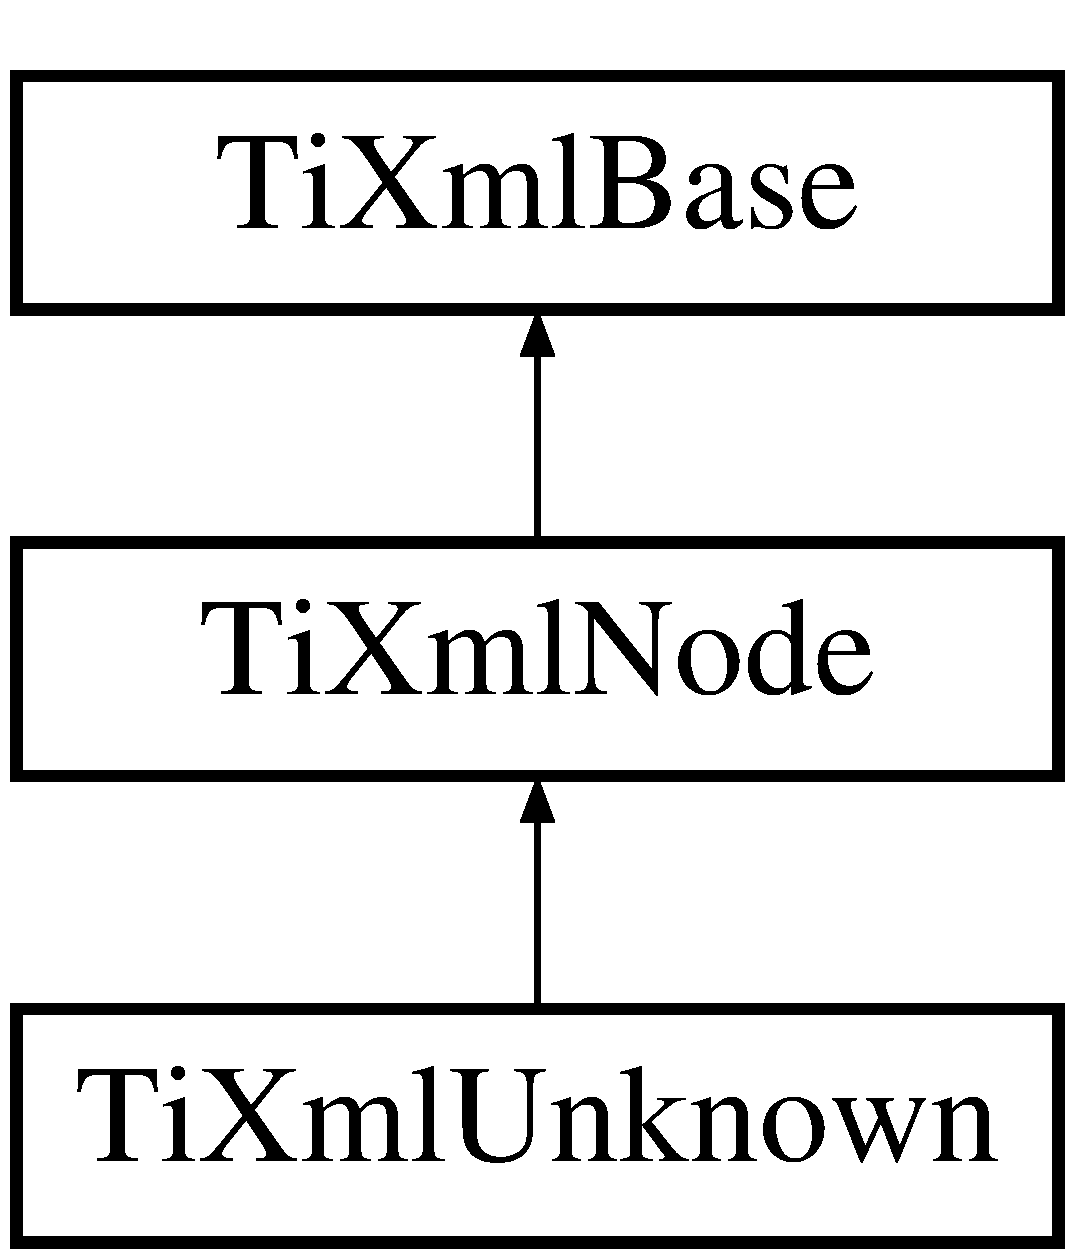
\includegraphics[height=3.000000cm]{class_ti_xml_unknown}
\end{center}
\end{figure}
\subsection*{Public Member Functions}
\begin{DoxyCompactItemize}
\item 
\mbox{\Hypertarget{class_ti_xml_unknown_abe798ff4feea31474850c7f0de6bdf5e}\label{class_ti_xml_unknown_abe798ff4feea31474850c7f0de6bdf5e}} 
{\bfseries Ti\+Xml\+Unknown} (const \hyperlink{class_ti_xml_unknown}{Ti\+Xml\+Unknown} \&copy)
\item 
\mbox{\Hypertarget{class_ti_xml_unknown_a60560b5aacb4bdc8b2b5f02f0a99c5c0}\label{class_ti_xml_unknown_a60560b5aacb4bdc8b2b5f02f0a99c5c0}} 
\hyperlink{class_ti_xml_unknown}{Ti\+Xml\+Unknown} \& {\bfseries operator=} (const \hyperlink{class_ti_xml_unknown}{Ti\+Xml\+Unknown} \&copy)
\item 
\mbox{\Hypertarget{class_ti_xml_unknown_a3dea7689de5b1931fd6657992948fde0}\label{class_ti_xml_unknown_a3dea7689de5b1931fd6657992948fde0}} 
virtual \hyperlink{class_ti_xml_node}{Ti\+Xml\+Node} $\ast$ \hyperlink{class_ti_xml_unknown_a3dea7689de5b1931fd6657992948fde0}{Clone} () const
\begin{DoxyCompactList}\small\item\em Creates a copy of this Unknown and returns it. \end{DoxyCompactList}\item 
virtual void \hyperlink{class_ti_xml_unknown_a5793fbc48ab3419783c0e866ca2d334e}{Print} (F\+I\+LE $\ast$cfile, int depth) const
\item 
\mbox{\Hypertarget{class_ti_xml_unknown_aa51c2694e4177b5f0b5429ee5a81b58d}\label{class_ti_xml_unknown_aa51c2694e4177b5f0b5429ee5a81b58d}} 
virtual const char $\ast$ {\bfseries Parse} (const char $\ast$p, \hyperlink{class_ti_xml_parsing_data}{Ti\+Xml\+Parsing\+Data} $\ast$data, Ti\+Xml\+Encoding encoding)
\item 
\mbox{\Hypertarget{class_ti_xml_unknown_a0d08dc16fc9ce16140ccaefbc35f6ea6}\label{class_ti_xml_unknown_a0d08dc16fc9ce16140ccaefbc35f6ea6}} 
virtual const \hyperlink{class_ti_xml_unknown}{Ti\+Xml\+Unknown} $\ast$ \hyperlink{class_ti_xml_unknown_a0d08dc16fc9ce16140ccaefbc35f6ea6}{To\+Unknown} () const
\begin{DoxyCompactList}\small\item\em Cast to a more defined type. Will return null not of the requested type. \end{DoxyCompactList}\item 
\mbox{\Hypertarget{class_ti_xml_unknown_a67c9fd22940e8c47f706a72cdd2e332c}\label{class_ti_xml_unknown_a67c9fd22940e8c47f706a72cdd2e332c}} 
virtual \hyperlink{class_ti_xml_unknown}{Ti\+Xml\+Unknown} $\ast$ \hyperlink{class_ti_xml_unknown_a67c9fd22940e8c47f706a72cdd2e332c}{To\+Unknown} ()
\begin{DoxyCompactList}\small\item\em Cast to a more defined type. Will return null not of the requested type. \end{DoxyCompactList}\item 
virtual bool \hyperlink{class_ti_xml_unknown_aafdf1b2d4f561979c7907bad91004999}{Accept} (\hyperlink{class_ti_xml_visitor}{Ti\+Xml\+Visitor} $\ast$content) const
\end{DoxyCompactItemize}
\subsection*{Protected Member Functions}
\begin{DoxyCompactItemize}
\item 
\mbox{\Hypertarget{class_ti_xml_unknown_afeb334446bcbe13ce15131e1629712be}\label{class_ti_xml_unknown_afeb334446bcbe13ce15131e1629712be}} 
void {\bfseries Copy\+To} (\hyperlink{class_ti_xml_unknown}{Ti\+Xml\+Unknown} $\ast$target) const
\item 
\mbox{\Hypertarget{class_ti_xml_unknown_adf84a317816124a2d7c7947d36170458}\label{class_ti_xml_unknown_adf84a317816124a2d7c7947d36170458}} 
virtual void {\bfseries Stream\+In} (std\+::istream $\ast$in, T\+I\+X\+M\+L\+\_\+\+S\+T\+R\+I\+NG $\ast$tag)
\end{DoxyCompactItemize}
\subsection*{Additional Inherited Members}


\subsection{Detailed Description}
Any tag that tiny\+Xml doesn\textquotesingle{}t recognize is saved as an unknown. It is a tag of text, but should not be modified. It will be written back to the X\+ML, unchanged, when the file is saved.

D\+TD tags get thrown into Ti\+Xml\+Unknowns. 

\subsection{Member Function Documentation}
\mbox{\Hypertarget{class_ti_xml_unknown_aafdf1b2d4f561979c7907bad91004999}\label{class_ti_xml_unknown_aafdf1b2d4f561979c7907bad91004999}} 
\index{Ti\+Xml\+Unknown@{Ti\+Xml\+Unknown}!Accept@{Accept}}
\index{Accept@{Accept}!Ti\+Xml\+Unknown@{Ti\+Xml\+Unknown}}
\subsubsection{\texorpdfstring{Accept()}{Accept()}}
{\footnotesize\ttfamily bool Ti\+Xml\+Unknown\+::\+Accept (\begin{DoxyParamCaption}\item[{\hyperlink{class_ti_xml_visitor}{Ti\+Xml\+Visitor} $\ast$}]{content }\end{DoxyParamCaption}) const\hspace{0.3cm}{\ttfamily [virtual]}}

Walk the X\+ML tree visiting this node and all of its children. 

Implements \hyperlink{class_ti_xml_node_acc0f88b7462c6cb73809d410a4f5bb86}{Ti\+Xml\+Node}.

\mbox{\Hypertarget{class_ti_xml_unknown_a5793fbc48ab3419783c0e866ca2d334e}\label{class_ti_xml_unknown_a5793fbc48ab3419783c0e866ca2d334e}} 
\index{Ti\+Xml\+Unknown@{Ti\+Xml\+Unknown}!Print@{Print}}
\index{Print@{Print}!Ti\+Xml\+Unknown@{Ti\+Xml\+Unknown}}
\subsubsection{\texorpdfstring{Print()}{Print()}}
{\footnotesize\ttfamily void Ti\+Xml\+Unknown\+::\+Print (\begin{DoxyParamCaption}\item[{F\+I\+LE $\ast$}]{cfile,  }\item[{int}]{depth }\end{DoxyParamCaption}) const\hspace{0.3cm}{\ttfamily [virtual]}}

All Tiny\+Xml classes can print themselves to a filestream or the string class (\hyperlink{class_ti_xml_string}{Ti\+Xml\+String} in non-\/\+S\+TL mode, std\+::string in S\+TL mode.) Either or both cfile and str can be null.

This is a formatted print, and will insert tabs and newlines.

(For an unformatted stream, use the $<$$<$ operator.) 

Implements \hyperlink{class_ti_xml_base_a0de56b3f2ef14c65091a3b916437b512}{Ti\+Xml\+Base}.



The documentation for this class was generated from the following files\+:\begin{DoxyCompactItemize}
\item 
utility/tiny\+\_\+xml/tinyxml.\+h\item 
utility/tiny\+\_\+xml/tinyxml.\+cpp\item 
utility/tiny\+\_\+xml/tinyxmlparser.\+cpp\end{DoxyCompactItemize}

\hypertarget{class_ti_xml_visitor}{}\section{Ti\+Xml\+Visitor Class Reference}
\label{class_ti_xml_visitor}\index{Ti\+Xml\+Visitor@{Ti\+Xml\+Visitor}}


{\ttfamily \#include $<$tinyxml.\+h$>$}

Inheritance diagram for Ti\+Xml\+Visitor\+:\begin{figure}[H]
\begin{center}
\leavevmode
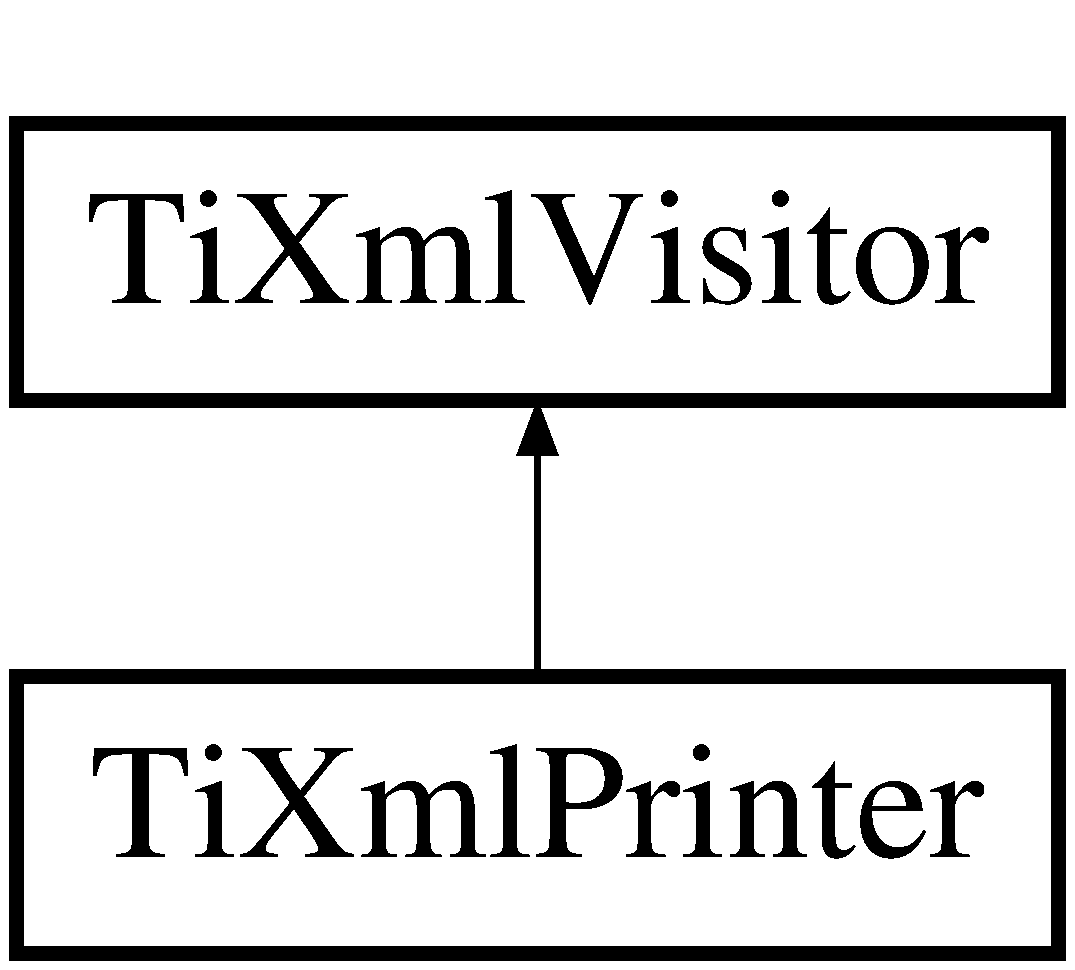
\includegraphics[height=2.000000cm]{class_ti_xml_visitor}
\end{center}
\end{figure}
\subsection*{Public Member Functions}
\begin{DoxyCompactItemize}
\item 
\hypertarget{class_ti_xml_visitor_a07baecb52dd7d8716ae2a48ad0956ee0}{}\label{class_ti_xml_visitor_a07baecb52dd7d8716ae2a48ad0956ee0} 
virtual bool \hyperlink{class_ti_xml_visitor_a07baecb52dd7d8716ae2a48ad0956ee0}{Visit\+Enter} (const \hyperlink{class_ti_xml_document}{Ti\+Xml\+Document} \&)
\begin{DoxyCompactList}\small\item\em Visit a document. \end{DoxyCompactList}\item 
\hypertarget{class_ti_xml_visitor_aa0ade4f27087447e93974e975c3246ad}{}\label{class_ti_xml_visitor_aa0ade4f27087447e93974e975c3246ad} 
virtual bool \hyperlink{class_ti_xml_visitor_aa0ade4f27087447e93974e975c3246ad}{Visit\+Exit} (const \hyperlink{class_ti_xml_document}{Ti\+Xml\+Document} \&)
\begin{DoxyCompactList}\small\item\em Visit a document. \end{DoxyCompactList}\item 
\hypertarget{class_ti_xml_visitor_af6c6178ffa517bbdba95d70490875fff}{}\label{class_ti_xml_visitor_af6c6178ffa517bbdba95d70490875fff} 
virtual bool \hyperlink{class_ti_xml_visitor_af6c6178ffa517bbdba95d70490875fff}{Visit\+Enter} (const \hyperlink{class_ti_xml_element}{Ti\+Xml\+Element} \&, const \hyperlink{class_ti_xml_attribute}{Ti\+Xml\+Attribute} $\ast$)
\begin{DoxyCompactList}\small\item\em Visit an element. \end{DoxyCompactList}\item 
\hypertarget{class_ti_xml_visitor_aec2b1f8116226d52f3a1b95dafd3a32c}{}\label{class_ti_xml_visitor_aec2b1f8116226d52f3a1b95dafd3a32c} 
virtual bool \hyperlink{class_ti_xml_visitor_aec2b1f8116226d52f3a1b95dafd3a32c}{Visit\+Exit} (const \hyperlink{class_ti_xml_element}{Ti\+Xml\+Element} \&)
\begin{DoxyCompactList}\small\item\em Visit an element. \end{DoxyCompactList}\item 
\hypertarget{class_ti_xml_visitor_afad71c71ce6473fb9b4b64cd92de4a19}{}\label{class_ti_xml_visitor_afad71c71ce6473fb9b4b64cd92de4a19} 
virtual bool \hyperlink{class_ti_xml_visitor_afad71c71ce6473fb9b4b64cd92de4a19}{Visit} (const \hyperlink{class_ti_xml_declaration}{Ti\+Xml\+Declaration} \&)
\begin{DoxyCompactList}\small\item\em Visit a declaration. \end{DoxyCompactList}\item 
\hypertarget{class_ti_xml_visitor_a399b8ebca5cd14664974a32d2ce029e5}{}\label{class_ti_xml_visitor_a399b8ebca5cd14664974a32d2ce029e5} 
virtual bool \hyperlink{class_ti_xml_visitor_a399b8ebca5cd14664974a32d2ce029e5}{Visit} (const \hyperlink{class_ti_xml_text}{Ti\+Xml\+Text} \&)
\begin{DoxyCompactList}\small\item\em Visit a text node. \end{DoxyCompactList}\item 
\hypertarget{class_ti_xml_visitor_a53a60e7a528627b31af3161972cc7fa2}{}\label{class_ti_xml_visitor_a53a60e7a528627b31af3161972cc7fa2} 
virtual bool \hyperlink{class_ti_xml_visitor_a53a60e7a528627b31af3161972cc7fa2}{Visit} (const \hyperlink{class_ti_xml_comment}{Ti\+Xml\+Comment} \&)
\begin{DoxyCompactList}\small\item\em Visit a comment node. \end{DoxyCompactList}\item 
\hypertarget{class_ti_xml_visitor_a7e284d607d275c51dac1adb58159ce28}{}\label{class_ti_xml_visitor_a7e284d607d275c51dac1adb58159ce28} 
virtual bool \hyperlink{class_ti_xml_visitor_a7e284d607d275c51dac1adb58159ce28}{Visit} (const \hyperlink{class_ti_xml_unknown}{Ti\+Xml\+Unknown} \&)
\begin{DoxyCompactList}\small\item\em Visit an unknown node. \end{DoxyCompactList}\end{DoxyCompactItemize}


\subsection{Detailed Description}
Implements the interface to the \char`\"{}\+Visitor pattern\char`\"{} (see the Accept() method.) If you call the Accept() method, it requires being passed a \hyperlink{class_ti_xml_visitor}{Ti\+Xml\+Visitor} class to handle callbacks. For nodes that contain other nodes (Document, Element) you will get called with a Visit\+Enter/\+Visit\+Exit pair. Nodes that are always leaves are simply called with \hyperlink{class_ti_xml_visitor_afad71c71ce6473fb9b4b64cd92de4a19}{Visit()}.

If you return \textquotesingle{}true\textquotesingle{} from a Visit method, recursive parsing will continue. If you return false, {\bfseries no children of this node or its sibilings} will be Visited.

All flavors of Visit methods have a default implementation that returns \textquotesingle{}true\textquotesingle{} (continue visiting). You need to only override methods that are interesting to you.

Generally Accept() is called on the \hyperlink{class_ti_xml_document}{Ti\+Xml\+Document}, although all nodes suppert Visiting.

You should never change the document from a callback.

\begin{DoxySeeAlso}{See also}
\hyperlink{class_ti_xml_node_acc0f88b7462c6cb73809d410a4f5bb86}{Ti\+Xml\+Node\+::\+Accept()} 
\end{DoxySeeAlso}


The documentation for this class was generated from the following file\+:\begin{DoxyCompactItemize}
\item 
utility/tiny\+\_\+xml/tinyxml.\+h\end{DoxyCompactItemize}

\hypertarget{class_view}{}\section{View Class Reference}
\label{class_view}\index{View@{View}}


Class controlling user interface.  




{\ttfamily \#include $<$view.\+h$>$}

Inheritance diagram for View\+:\begin{figure}[H]
\begin{center}
\leavevmode
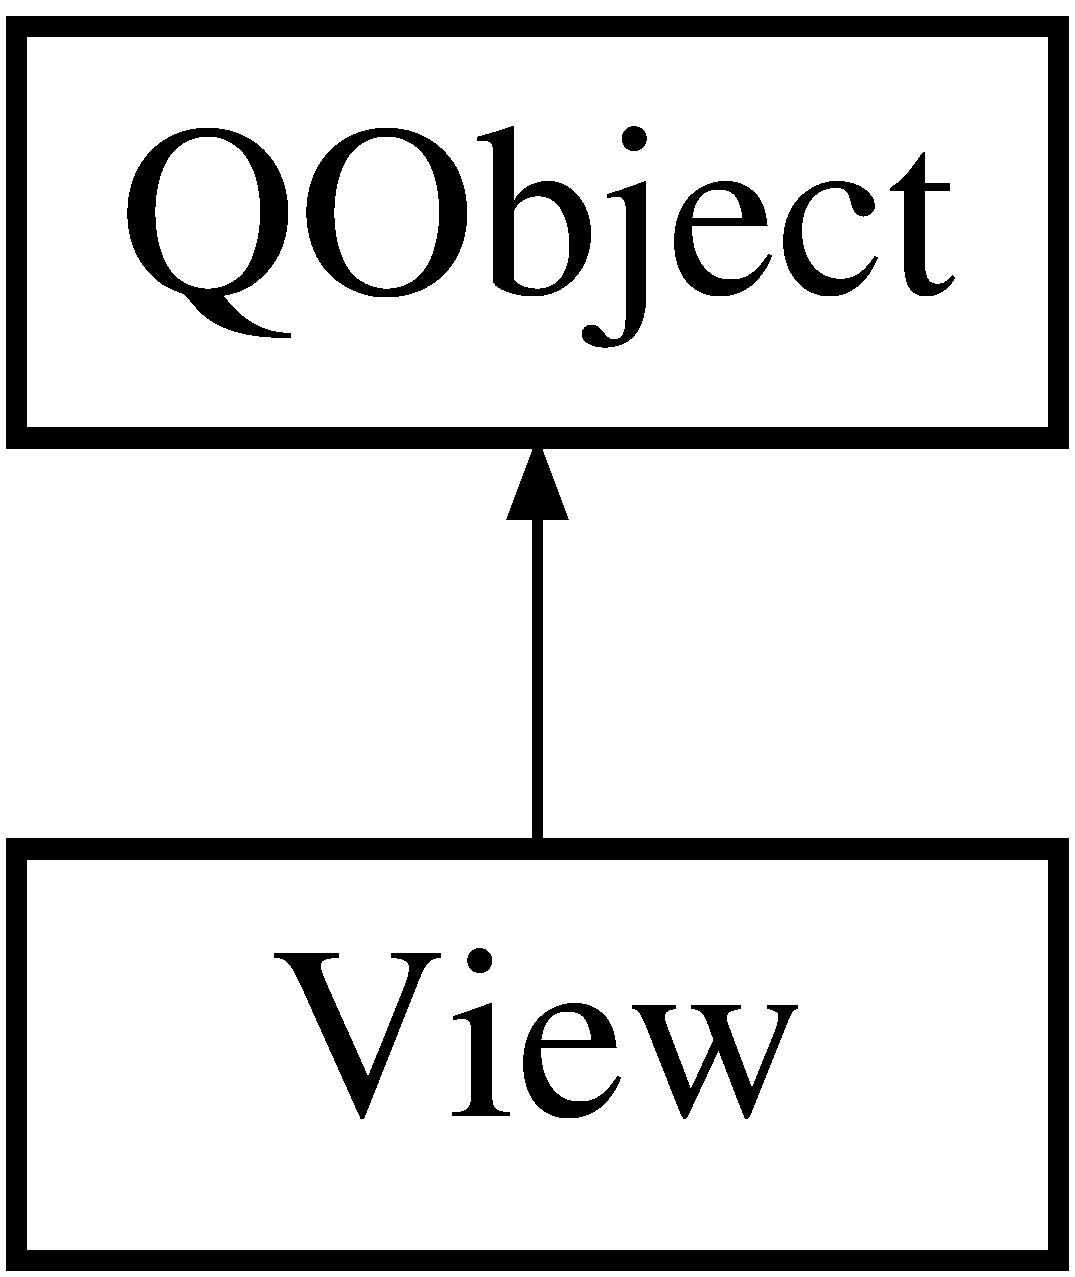
\includegraphics[height=2.000000cm]{class_view}
\end{center}
\end{figure}
\subsection*{Public Slots}
\begin{DoxyCompactItemize}
\item 
\hypertarget{class_view_ae947cd6d87306563e8827d80448c1f28}{}\label{class_view_ae947cd6d87306563e8827d80448c1f28} 
void {\bfseries draw\+Base\+Chart} (const std\+::vector$<$ double $>$ \&dataX, const std\+::vector$<$ double $>$ \&dataY)
\item 
\hypertarget{class_view_ad0df9f601ff799e4555e4662e1b0352c}{}\label{class_view_ad0df9f601ff799e4555e4662e1b0352c} 
void {\bfseries draw\+Optimized\+Chart} (const std\+::vector$<$ double $>$ \&dataX, const std\+::vector$<$ double $>$ \&dataY)
\item 
\hypertarget{class_view_a81a7e65b2a53ad30ce94b42c214dc3ef}{}\label{class_view_a81a7e65b2a53ad30ce94b42c214dc3ef} 
void {\bfseries draw\+Genetic\+Plot} (const std\+::vector$<$ double $>$ \&dataX, const std\+::vector$<$ double $>$ \&dataY)
\item 
\hypertarget{class_view_a717cea2de9e99ba58fe35a574bb56554}{}\label{class_view_a717cea2de9e99ba58fe35a574bb56554} 
void {\bfseries buttons\+Clicked} (Q\+String name)
\item 
\hypertarget{class_view_a2291d8c957e0095b57d76bb247d6a915}{}\label{class_view_a2291d8c957e0095b57d76bb247d6a915} 
void {\bfseries get\+Fitness\+Parameters\+Label} (\hyperlink{struct_aviation_profile_parameters}{Aviation\+Profile\+Parameters} data)
\item 
\hypertarget{class_view_a47d43d8644c74f17993a4ce2754e5be7}{}\label{class_view_a47d43d8644c74f17993a4ce2754e5be7} 
void {\bfseries get\+Base\+Profile\+Values} (\hyperlink{struct_aviation_profile_parameters}{Aviation\+Profile\+Parameters} data)
\item 
\hypertarget{class_view_a2556a1b48f4c638f752b5e22e6044adb}{}\label{class_view_a2556a1b48f4c638f752b5e22e6044adb} 
void {\bfseries set\+Optimizer\+Settings} ()
\end{DoxyCompactItemize}
\subsection*{Signals}
\begin{DoxyCompactItemize}
\item 
\hypertarget{class_view_a17beef462b991abf311bcaeacfe3b7d8}{}\label{class_view_a17beef462b991abf311bcaeacfe3b7d8} 
void {\bfseries set\+Target\+Profile\+Values} (\hyperlink{struct_aviation_profile_parameters}{Aviation\+Profile\+Parameters} data)
\item 
\hypertarget{class_view_a29594d0b3b97def30b5586ddaf11d288}{}\label{class_view_a29594d0b3b97def30b5586ddaf11d288} 
void {\bfseries redirect\+Path\+To\+Base\+Profile} (std\+::string path)
\item 
\hypertarget{class_view_ae3633aa70a59017a0f3728a9a7e455bd}{}\label{class_view_ae3633aa70a59017a0f3728a9a7e455bd} 
void {\bfseries stop\+Simulation} ()
\end{DoxyCompactItemize}
\subsection*{Public Member Functions}
\begin{DoxyCompactItemize}
\item 
\hypertarget{class_view_adc973dbae490e2040f813633e00b6e6f}{}\label{class_view_adc973dbae490e2040f813633e00b6e6f} 
{\bfseries View} (\hyperlink{class_model}{Model} $\ast$model)
\item 
\hypertarget{class_view_aea935ceb9d8f3d9b0153c6b9890c903f}{}\label{class_view_aea935ceb9d8f3d9b0153c6b9890c903f} 
void {\bfseries enable\+Progress\+Bar} ()
\item 
\hypertarget{class_view_a211d282520bc0d5373e3a2f57a611ffc}{}\label{class_view_a211d282520bc0d5373e3a2f57a611ffc} 
void {\bfseries disable\+Progress\+Bar} ()
\end{DoxyCompactItemize}


\subsection{Detailed Description}
Class controlling user interface. 

\hyperlink{class_view}{View} consists all components and methods responsible for communication with user and redirect information to model of application. 

The documentation for this class was generated from the following files\+:\begin{DoxyCompactItemize}
\item 
gui/\hyperlink{view_8h}{view.\+h}\item 
gui/view.\+cpp\end{DoxyCompactItemize}

\chapter{File Documentation}
\hypertarget{gui__objects_8h}{}\section{gui/gui\+\_\+objects.h File Reference}
\label{gui__objects_8h}\index{gui/gui\+\_\+objects.\+h@{gui/gui\+\_\+objects.\+h}}


This header file contains all required objects represents user interface.  


{\ttfamily \#include $<$Q\+Object$>$}\newline
{\ttfamily \#include $<$Q\+Dialog$>$}\newline
{\ttfamily \#include $<$vector$>$}\newline
\subsection*{Classes}
\begin{DoxyCompactItemize}
\item 
struct \hyperlink{struct_component}{Component}
\item 
struct \hyperlink{struct_main_window_objects}{Main\+Window\+Objects}
\item 
struct \hyperlink{struct_settings_objects}{Settings\+Objects}
\item 
struct \hyperlink{struct_plot}{Plot}
\end{DoxyCompactItemize}


\subsection{Detailed Description}
This header file contains all required objects represents user interface. 

\begin{DoxyAuthor}{Author}
Jakub Polaczek \& Hubert Buczyński 
\end{DoxyAuthor}
\begin{DoxyDate}{Date}
05/06/2017 
\end{DoxyDate}

\hypertarget{plot__dialog_8h}{}\section{gui/plot\+\_\+dialog.h File Reference}
\label{plot__dialog_8h}\index{gui/plot\+\_\+dialog.\+h@{gui/plot\+\_\+dialog.\+h}}


This header file contains all required functions to draw progress plot of genethic algorithm.  


{\ttfamily \#include $<$Q\+Qml\+Application\+Engine$>$}\newline
{\ttfamily \#include $<$Q\+Qml\+Component$>$}\newline
{\ttfamily \#include $<$vector$>$}\newline
{\ttfamily \#include $<$Q\+Object$>$}\newline
{\ttfamily \#include \char`\"{}gui/gui\+\_\+objects.\+h\char`\"{}}\newline
\subsection*{Classes}
\begin{DoxyCompactItemize}
\item 
class \hyperlink{class_plot_dialog}{Plot\+Dialog}
\begin{DoxyCompactList}\small\item\em Class provides drawing chart in external dialog. \end{DoxyCompactList}\end{DoxyCompactItemize}


\subsection{Detailed Description}
This header file contains all required functions to draw progress plot of genethic algorithm. 

\begin{DoxyAuthor}{Author}
Jakub Polaczek \& Hubert Buczyński 
\end{DoxyAuthor}
\begin{DoxyDate}{Date}
05/06/2017 
\end{DoxyDate}

\hypertarget{settings__dialog_8h}{}\section{gui/settings\+\_\+dialog.h File Reference}
\label{settings__dialog_8h}\index{gui/settings\+\_\+dialog.\+h@{gui/settings\+\_\+dialog.\+h}}


This header file consists settings dialog class.  


{\ttfamily \#include $<$Q\+Qml\+Application\+Engine$>$}\newline
{\ttfamily \#include $<$Q\+Qml\+Component$>$}\newline
{\ttfamily \#include \char`\"{}gui/gui\+\_\+objects.\+h\char`\"{}}\newline
\subsection*{Classes}
\begin{DoxyCompactItemize}
\item 
class \hyperlink{class_settings_dialog}{Settings\+Dialog}
\begin{DoxyCompactList}\small\item\em The class takes care of genetic algorithm\textquotesingle{}s settings obtain from user. \end{DoxyCompactList}\end{DoxyCompactItemize}


\subsection{Detailed Description}
This header file consists settings dialog class. 

\begin{DoxyAuthor}{Author}
Jakub Polaczek \& Hubert Buczyński 
\end{DoxyAuthor}
\begin{DoxyDate}{Date}
05/06/2017 
\end{DoxyDate}

\hypertarget{view_8h}{}\section{gui/view.h File Reference}
\label{view_8h}\index{gui/view.\+h@{gui/view.\+h}}


\hyperlink{class_view}{View} class maintains user interface.  


{\ttfamily \#include $<$Q\+Application$>$}\newline
{\ttfamily \#include $<$Q\+Qml\+Application\+Engine$>$}\newline
{\ttfamily \#include $<$Q\+Qml\+Component$>$}\newline
{\ttfamily \#include \char`\"{}model/profile\+\_\+parameters.\+h\char`\"{}}\newline
{\ttfamily \#include \char`\"{}model/model.\+h\char`\"{}}\newline
{\ttfamily \#include \char`\"{}gui/settings\+\_\+dialog.\+h\char`\"{}}\newline
{\ttfamily \#include \char`\"{}gui/plot\+\_\+dialog.\+h\char`\"{}}\newline
\subsection*{Classes}
\begin{DoxyCompactItemize}
\item 
class \hyperlink{class_view}{View}
\begin{DoxyCompactList}\small\item\em Class controlling user interface. \end{DoxyCompactList}\end{DoxyCompactItemize}


\subsection{Detailed Description}
\hyperlink{class_view}{View} class maintains user interface. 

\begin{DoxyAuthor}{Author}
Jakub Polaczek \& Hubert Buczyński 
\end{DoxyAuthor}
\begin{DoxyDate}{Date}
05/06/2017 
\end{DoxyDate}

\hypertarget{model_8h}{}\section{model/model.h File Reference}
\label{model_8h}\index{model/model.\+h@{model/model.\+h}}


The class is responsible for management of an application\textquotesingle{}s back-\/end.  


{\ttfamily \#include $<$vector$>$}\newline
{\ttfamily \#include $<$Q\+Object$>$}\newline
{\ttfamily \#include \char`\"{}utility/log\+\_\+writer.\+h\char`\"{}}\newline
{\ttfamily \#include \char`\"{}utility/configuration\+\_\+reader.\+h\char`\"{}}\newline
{\ttfamily \#include \char`\"{}utility/config.\+h\char`\"{}}\newline
{\ttfamily \#include \char`\"{}model/profile\+\_\+parameters.\+h\char`\"{}}\newline
{\ttfamily \#include \char`\"{}optimizer/genetic/genetic.\+h\char`\"{}}\newline
\subsection*{Classes}
\begin{DoxyCompactItemize}
\item 
class \hyperlink{class_model}{Model}
\begin{DoxyCompactList}\small\item\em Class manage G\+UI and genethic algorithm. \end{DoxyCompactList}\end{DoxyCompactItemize}


\subsection{Detailed Description}
The class is responsible for management of an application\textquotesingle{}s back-\/end. 

\begin{DoxyAuthor}{Author}
Jakub Polaczek \& Hubert Buczyński 
\end{DoxyAuthor}
\begin{DoxyDate}{Date}
05/06/2017 
\end{DoxyDate}

\hypertarget{profile__parameters_8h}{}\section{model/profile\+\_\+parameters.h File Reference}
\label{profile__parameters_8h}\index{model/profile\+\_\+parameters.\+h@{model/profile\+\_\+parameters.\+h}}


This header file contains structure represenets airfoil parameters.  


\subsection*{Classes}
\begin{DoxyCompactItemize}
\item 
struct \hyperlink{struct_aviation_profile_parameters}{Aviation\+Profile\+Parameters}
\begin{DoxyCompactList}\small\item\em Struct consists airfoil basic parameters. \end{DoxyCompactList}\end{DoxyCompactItemize}


\subsection{Detailed Description}
This header file contains structure represenets airfoil parameters. 

\begin{DoxyAuthor}{Author}
Jakub Polaczek \& Hubert Buczyński 
\end{DoxyAuthor}
\begin{DoxyDate}{Date}
05/06/2017 
\end{DoxyDate}

\hypertarget{airfoil__optimizer_8h}{}\section{optimizer/airfoil\+\_\+optimizer.h File Reference}
\label{airfoil__optimizer_8h}\index{optimizer/airfoil\+\_\+optimizer.\+h@{optimizer/airfoil\+\_\+optimizer.\+h}}


Interface class for various optimizers.  


{\ttfamily \#include \char`\"{}optimizer/geometry.\+h\char`\"{}}\newline
{\ttfamily \#include $<$Q\+Object$>$}\newline
\subsection*{Classes}
\begin{DoxyCompactItemize}
\item 
class \hyperlink{class_airfoil_optimizer}{Airfoil\+Optimizer}
\item 
class \hyperlink{class_dud_optimizer}{Dud\+Optimizer}
\end{DoxyCompactItemize}


\subsection{Detailed Description}
Interface class for various optimizers. 

\begin{DoxyAuthor}{Author}
Jakub Polaczek \& Hubert Buczyński 
\end{DoxyAuthor}
\begin{DoxyDate}{Date}
05/06/2017 
\end{DoxyDate}

\hypertarget{fitness_8h}{}\section{optimizer/genetic/fitness.h File Reference}
\label{fitness_8h}\index{optimizer/genetic/fitness.\+h@{optimizer/genetic/fitness.\+h}}


This header file contains function to calculate fitness od specific genome.  


{\ttfamily \#include \char`\"{}optimizer/simulation\+\_\+results.\+h\char`\"{}}\newline
{\ttfamily \#include \char`\"{}utility/config.\+h\char`\"{}}\newline
\subsection*{Classes}
\begin{DoxyCompactItemize}
\item 
class \hyperlink{class_fitness_model}{Fitness\+Model}
\begin{DoxyCompactList}\small\item\em Class maintain fitness function for genetic algorithm. \end{DoxyCompactList}\end{DoxyCompactItemize}


\subsection{Detailed Description}
This header file contains function to calculate fitness od specific genome. 

\begin{DoxyAuthor}{Author}
Jakub Polaczek \& Hubert Buczyński 
\end{DoxyAuthor}
\begin{DoxyDate}{Date}
05/06/2017 
\end{DoxyDate}

\hypertarget{genetic_8h}{}\section{optimizer/genetic/genetic.h File Reference}
\label{genetic_8h}\index{optimizer/genetic/genetic.\+h@{optimizer/genetic/genetic.\+h}}


File consists header for genetic algorithm.  


{\ttfamily \#include $<$vector$>$}\newline
{\ttfamily \#include $<$algorithm$>$}\newline
{\ttfamily \#include $<$Q\+Object$>$}\newline
{\ttfamily \#include \char`\"{}optimizer/airfoil\+\_\+optimizer.\+h\char`\"{}}\newline
{\ttfamily \#include \char`\"{}xfoil/simulation.\+h\char`\"{}}\newline
{\ttfamily \#include \char`\"{}optimizer/genetic/genome.\+h\char`\"{}}\newline
{\ttfamily \#include \char`\"{}optimizer/genetic/genome\+\_\+scrambler.\+h\char`\"{}}\newline
{\ttfamily \#include \char`\"{}utility/config.\+h\char`\"{}}\newline
{\ttfamily \#include \char`\"{}model/profile\+\_\+parameters.\+h\char`\"{}}\newline
\subsection*{Classes}
\begin{DoxyCompactItemize}
\item 
class \hyperlink{class_genetic_optimizer}{Genetic\+Optimizer}
\begin{DoxyCompactList}\small\item\em Class contains implementation of the genetic algorithm. \end{DoxyCompactList}\end{DoxyCompactItemize}


\subsection{Detailed Description}
File consists header for genetic algorithm. 

\begin{DoxyAuthor}{Author}
Jakub Polaczek \& Hubert Buczyński 
\end{DoxyAuthor}
\begin{DoxyDate}{Date}
05/06/2017 
\end{DoxyDate}

\hypertarget{genome_8h}{}\section{optimizer/genetic/genome.h File Reference}
\label{genome_8h}\index{optimizer/genetic/genome.\+h@{optimizer/genetic/genome.\+h}}


Class providing basic 2D airfoil geometry representation.  


{\ttfamily \#include \char`\"{}optimizer/geometry.\+h\char`\"{}}\newline
{\ttfamily \#include \char`\"{}optimizer/genetic/fitness.\+h\char`\"{}}\newline
{\ttfamily \#include $<$random$>$}\newline
\subsection*{Classes}
\begin{DoxyCompactItemize}
\item 
class \hyperlink{class_genome}{Genome}
\end{DoxyCompactItemize}


\subsection{Detailed Description}
Class providing basic 2D airfoil geometry representation. 

\begin{DoxyAuthor}{Author}
Jakub Polaczek \& Hubert Buczyński 
\end{DoxyAuthor}
\begin{DoxyDate}{Date}
05/06/2017 
\end{DoxyDate}

\hypertarget{genome__scrambler_8h}{}\section{optimizer/genetic/genome\+\_\+scrambler.h File Reference}
\label{genome__scrambler_8h}\index{optimizer/genetic/genome\+\_\+scrambler.\+h@{optimizer/genetic/genome\+\_\+scrambler.\+h}}


File providing methods to genome mutation and crossover.  


{\ttfamily \#include \char`\"{}optimizer/genetic/genome.\+h\char`\"{}}\newline
\subsection*{Classes}
\begin{DoxyCompactItemize}
\item 
class \hyperlink{class_genome_scrambler}{Genome\+Scrambler}
\begin{DoxyCompactList}\small\item\em Representation of abstract class. \end{DoxyCompactList}\item 
class \hyperlink{class_dud_scrambler}{Dud\+Scrambler}
\begin{DoxyCompactList}\small\item\em Class provides methods to genome reproduction. \end{DoxyCompactList}\end{DoxyCompactItemize}


\subsection{Detailed Description}
File providing methods to genome mutation and crossover. 

\begin{DoxyAuthor}{Author}
Jakub Polaczek \& Hubert Buczyński 
\end{DoxyAuthor}
\begin{DoxyDate}{Date}
05/06/2017 
\end{DoxyDate}

\hypertarget{geometry_8h}{}\section{optimizer/geometry.h File Reference}
\label{geometry_8h}\index{optimizer/geometry.\+h@{optimizer/geometry.\+h}}


File consists representation of airfoil geometry.  


{\ttfamily \#include $<$vector$>$}\newline
{\ttfamily \#include $<$fstream$>$}\newline
{\ttfamily \#include $<$iostream$>$}\newline
{\ttfamily \#include $<$iterator$>$}\newline
{\ttfamily \#include $<$string$>$}\newline
{\ttfamily \#include \char`\"{}optimizer/simulation\+\_\+results.\+h\char`\"{}}\newline
{\ttfamily \#include \char`\"{}optimizer/geometry\+\_\+structures.\+h\char`\"{}}\newline
\subsection*{Classes}
\begin{DoxyCompactItemize}
\item 
class \hyperlink{class_geometry}{Geometry}
\begin{DoxyCompactList}\small\item\em Class providing necessary attributes for geometry calculation. \end{DoxyCompactList}\end{DoxyCompactItemize}


\subsection{Detailed Description}
File consists representation of airfoil geometry. 

\begin{DoxyAuthor}{Author}
Jakub Polaczek \& Hubert Buczyński 
\end{DoxyAuthor}
\begin{DoxyDate}{Date}
05/06/2017 
\end{DoxyDate}

\hypertarget{geometry__structures_8h}{}\section{optimizer/geometry\+\_\+structures.h File Reference}
\label{geometry__structures_8h}\index{optimizer/geometry\+\_\+structures.\+h@{optimizer/geometry\+\_\+structures.\+h}}


This header file contains all required structures to represent geometry\textquotesingle{}s coefficients.  


{\ttfamily \#include $<$cmath$>$}\newline
\subsection*{Classes}
\begin{DoxyCompactItemize}
\item 
struct \hyperlink{struct_airfoil_coefficients}{Airfoil\+Coefficients}
\item 
struct \hyperlink{struct_binary_airfoil_coefficients}{Binary\+Airfoil\+Coefficients}
\item 
class \hyperlink{class_point}{Point}
\end{DoxyCompactItemize}
\subsection*{Typedefs}
\begin{DoxyCompactItemize}
\item 
\hypertarget{geometry__structures_8h_a61902b37514c53f51a2fb8423db5ee36}{}\label{geometry__structures_8h_a61902b37514c53f51a2fb8423db5ee36} 
typedef std\+::uint8\+\_\+t {\bfseries byte}
\end{DoxyCompactItemize}
\subsection*{Functions}
\begin{DoxyCompactItemize}
\item 
\hypertarget{geometry__structures_8h_ad32019380665fdd1d07e75f3482544a3}{}\label{geometry__structures_8h_ad32019380665fdd1d07e75f3482544a3} 
bool {\bfseries operator==} (const \hyperlink{class_point}{Point} \&lhs, const \hyperlink{class_point}{Point} \&rhs)
\end{DoxyCompactItemize}


\subsection{Detailed Description}
This header file contains all required structures to represent geometry\textquotesingle{}s coefficients. 

\begin{DoxyAuthor}{Author}
Jakub Polaczek \& Hubert Buczyński 
\end{DoxyAuthor}
\begin{DoxyDate}{Date}
05/06/2017 
\end{DoxyDate}

\hypertarget{simulation__results_8h}{}\section{optimizer/simulation\+\_\+results.h File Reference}
\label{simulation__results_8h}\index{optimizer/simulation\+\_\+results.\+h@{optimizer/simulation\+\_\+results.\+h}}


Class containing simulation results from xfoil.  


{\ttfamily \#include $<$vector$>$}\newline
\subsection*{Classes}
\begin{DoxyCompactItemize}
\item 
class \hyperlink{class_sim_results}{Sim\+Results}
\item 
struct \hyperlink{struct_sim_results_1_1_result_entry}{Sim\+Results\+::\+Result\+Entry}
\begin{DoxyCompactList}\small\item\em Class containing simulation results from xfoil Structure for storing simulation results from xfoil panel optimizer. \end{DoxyCompactList}\item 
struct \hyperlink{struct_sim_results_1_1_polar_point}{Sim\+Results\+::\+Polar\+Point}
\end{DoxyCompactItemize}


\subsection{Detailed Description}
Class containing simulation results from xfoil. 

\begin{DoxyAuthor}{Author}
Jakub Polaczek \& Hubert Buczyński 
\end{DoxyAuthor}
\begin{DoxyDate}{Date}
05/06/2017 
\end{DoxyDate}

\hypertarget{config_8h}{}\section{utility/config.h File Reference}
\label{config_8h}\index{utility/config.\+h@{utility/config.\+h}}


Class containing parameters for the whole application.  


{\ttfamily \#include $<$map$>$}\newline
{\ttfamily \#include $<$boost/variant.\+hpp$>$}\newline
\subsection*{Classes}
\begin{DoxyCompactItemize}
\item 
class \hyperlink{class_config}{Config}
\begin{DoxyCompactList}\small\item\em Class containing application parameters. \end{DoxyCompactList}\item 
struct \hyperlink{struct_config_1_1_application_params}{Config\+::\+Application\+Params}
\item 
struct \hyperlink{struct_config_1_1_simulation_params}{Config\+::\+Simulation\+Params}
\item 
struct \hyperlink{struct_config_1_1_optimizer_params}{Config\+::\+Optimizer\+Params}
\item 
struct \hyperlink{struct_config_1_1_optimizer_params_1_1_fitness}{Config\+::\+Optimizer\+Params\+::\+Fitness}
\item 
struct \hyperlink{struct_config_1_1_optimizer_params_1_1_genetic_optimizer_params}{Config\+::\+Optimizer\+Params\+::\+Genetic\+Optimizer\+Params}
\end{DoxyCompactItemize}
\subsection*{Typedefs}
\begin{DoxyCompactItemize}
\item 
\mbox{\Hypertarget{config_8h_a97e423ec92a2c79e7526e60e8ccf1cf9}\label{config_8h_a97e423ec92a2c79e7526e60e8ccf1cf9}} 
typedef std\+::map$<$ std\+::string, boost\+::variant$<$ double, std\+::string, int $>$ $>$ {\bfseries Parameters}
\end{DoxyCompactItemize}


\subsection{Detailed Description}
Class containing parameters for the whole application. 

\begin{DoxyAuthor}{Author}
Jakub Polaczek \& Hubert Buczyński 
\end{DoxyAuthor}
\begin{DoxyDate}{Date}
05/06/2017 
\end{DoxyDate}

\hypertarget{configuration__reader_8h}{}\section{utility/configuration\+\_\+reader.h File Reference}
\label{configuration__reader_8h}\index{utility/configuration\+\_\+reader.\+h@{utility/configuration\+\_\+reader.\+h}}


Class containing methods to generate and load parameters from xml file.  


{\ttfamily \#include $<$string$>$}\newline
{\ttfamily \#include \char`\"{}tiny\+\_\+xml/tinystr.\+h\char`\"{}}\newline
{\ttfamily \#include \char`\"{}tiny\+\_\+xml/tinyxml.\+h\char`\"{}}\newline
{\ttfamily \#include \char`\"{}log\+\_\+writer.\+h\char`\"{}}\newline
{\ttfamily \#include \char`\"{}config.\+h\char`\"{}}\newline
\subsection*{Classes}
\begin{DoxyCompactItemize}
\item 
class \hyperlink{class_configuration_reader}{Configuration\+Reader}
\begin{DoxyCompactList}\small\item\em Class containing methods to generate and load parameters from xml file. \end{DoxyCompactList}\end{DoxyCompactItemize}


\subsection{Detailed Description}
Class containing methods to generate and load parameters from xml file. 

\begin{DoxyAuthor}{Author}
Jakub Polaczek \& Hubert Buczyński 
\end{DoxyAuthor}
\begin{DoxyDate}{Date}
05/06/2017 
\end{DoxyDate}

\hypertarget{log__writer_8h}{}\section{utility/log\+\_\+writer.h File Reference}
\label{log__writer_8h}\index{utility/log\+\_\+writer.\+h@{utility/log\+\_\+writer.\+h}}


File conists logger class. Logger is implemented as singleton.  


{\ttfamily \#include $<$fstream$>$}\newline
{\ttfamily \#include $<$string$>$}\newline
{\ttfamily \#include $<$mutex$>$}\newline
\subsection*{Classes}
\begin{DoxyCompactItemize}
\item 
class \hyperlink{class_log_writer}{Log\+Writer}
\begin{DoxyCompactList}\small\item\em Class containing methods add information about current state of application. \end{DoxyCompactList}\end{DoxyCompactItemize}


\subsection{Detailed Description}
File conists logger class. Logger is implemented as singleton. 

\begin{DoxyAuthor}{Author}
Jakub Polaczek \& Hubert Buczyński 
\end{DoxyAuthor}
\begin{DoxyDate}{Date}
05/06/2017 
\end{DoxyDate}

\hypertarget{time__manager_8h}{}\section{utility/time\+\_\+manager.h File Reference}
\label{time__manager_8h}\index{utility/time\+\_\+manager.\+h@{utility/time\+\_\+manager.\+h}}


Header file consists necessary methods to measure current time in application.  


{\ttfamily \#include $<$chrono$>$}\newline
{\ttfamily \#include $<$string$>$}\newline
\subsection*{Classes}
\begin{DoxyCompactItemize}
\item 
class \hyperlink{class_time_manager}{Time\+Manager}
\begin{DoxyCompactList}\small\item\em Class containing methods to measure time. \end{DoxyCompactList}\end{DoxyCompactItemize}


\subsection{Detailed Description}
Header file consists necessary methods to measure current time in application. 

\begin{DoxyAuthor}{Author}
Jakub Polaczek \& Hubert Buczyński 
\end{DoxyAuthor}
\begin{DoxyDate}{Date}
05/06/2017 
\end{DoxyDate}

\hypertarget{utility_8h}{}\section{utility/utility.h File Reference}
\label{utility_8h}\index{utility/utility.\+h@{utility/utility.\+h}}


This header file consists exception handler. Moreover it provides utility namespace to make basic operation on files and directories.  


{\ttfamily \#include $<$string$>$}\newline
\subsection*{Classes}
\begin{DoxyCompactItemize}
\item 
struct \hyperlink{struct_exception_handler}{Exception\+Handler}
\begin{DoxyCompactList}\small\item\em Exception Handler. \end{DoxyCompactList}\end{DoxyCompactItemize}
\subsection*{Functions}
\begin{DoxyCompactItemize}
\item 
\mbox{\Hypertarget{utility_8h_a47550720c8d006b01e209813a69f8d61}\label{utility_8h_a47550720c8d006b01e209813a69f8d61}} 
bool {\bfseries utility\+::create\+Directory\+Recursively} (const std\+::string \&directory)
\item 
\mbox{\Hypertarget{utility_8h_a4145c59333583b6d77809e119e0eba0c}\label{utility_8h_a4145c59333583b6d77809e119e0eba0c}} 
bool {\bfseries utility\+::file\+Exists} (std\+::string file)
\item 
\mbox{\Hypertarget{utility_8h_a8e13215730a864991856f24c51acd18f}\label{utility_8h_a8e13215730a864991856f24c51acd18f}} 
void {\bfseries utility\+::remove\+File} (std\+::string file)
\end{DoxyCompactItemize}


\subsection{Detailed Description}
This header file consists exception handler. Moreover it provides utility namespace to make basic operation on files and directories. 

\begin{DoxyAuthor}{Author}
Jakub Polaczek \& Hubert Buczyński 
\end{DoxyAuthor}
\begin{DoxyDate}{Date}
05/06/2017 
\end{DoxyDate}

\hypertarget{qsimulation_8h}{}\section{xfoil/qsimulation.h File Reference}
\label{qsimulation_8h}\index{xfoil/qsimulation.\+h@{xfoil/qsimulation.\+h}}


QT based implementation for handling process command inputs.  


{\ttfamily \#include $<$qprocess.\+h$>$}\newline
{\ttfamily \#include $<$chrono$>$}\newline
{\ttfamily \#include \char`\"{}simulation\+\_\+proxy.\+h\char`\"{}}\newline
{\ttfamily \#include \char`\"{}utility/config.\+h\char`\"{}}\newline
\subsection*{Classes}
\begin{DoxyCompactItemize}
\item 
class \hyperlink{class_q_simulation_proxy}{Q\+Simulation\+Proxy}
\end{DoxyCompactItemize}


\subsection{Detailed Description}
QT based implementation for handling process command inputs. 

\begin{DoxyAuthor}{Author}
Jakub Polaczek \& Hubert Buczyński 
\end{DoxyAuthor}
\begin{DoxyDate}{Date}
05/06/2017 
\end{DoxyDate}

\hypertarget{simulation_8h}{}\section{xfoil/simulation.h File Reference}
\label{simulation_8h}\index{xfoil/simulation.\+h@{xfoil/simulation.\+h}}


This header file contains tools to maintain communication with external program -\/ X\+F\+O\+IL.  


{\ttfamily \#include $<$vector$>$}\newline
{\ttfamily \#include $<$iostream$>$}\newline
{\ttfamily \#include $<$string$>$}\newline
{\ttfamily \#include $<$sstream$>$}\newline
{\ttfamily \#include $<$fstream$>$}\newline
{\ttfamily \#include $<$exception$>$}\newline
{\ttfamily \#include \char`\"{}optimizer/simulation\+\_\+results.\+h\char`\"{}}\newline
{\ttfamily \#include \char`\"{}xfoil/simulation\+\_\+proxy.\+h\char`\"{}}\newline
{\ttfamily \#include \char`\"{}xfoil/qsimulation.\+h\char`\"{}}\newline
{\ttfamily \#include \char`\"{}utility/utility.\+h\char`\"{}}\newline
{\ttfamily \#include \char`\"{}utility/config.\+h\char`\"{}}\newline
{\ttfamily \#include $<$qthread.\+h$>$}\newline
{\ttfamily \#include $<$qtimer.\+h$>$}\newline
{\ttfamily \#include $<$qmutex.\+h$>$}\newline
{\ttfamily \#include $<$queue$>$}\newline
\subsection*{Classes}
\begin{DoxyCompactItemize}
\item 
class \hyperlink{class_simulation_handler}{Simulation\+Handler}
\begin{DoxyCompactList}\small\item\em Class controlling execution single simulation tool using proxy interface. \end{DoxyCompactList}\item 
struct \hyperlink{struct_task}{Task}
\begin{DoxyCompactList}\small\item\em Object encapsulating single task for \hyperlink{class_scheduler_worker}{Scheduler\+Worker}. \end{DoxyCompactList}\item 
class \hyperlink{class_scheduler_worker}{Scheduler\+Worker}
\begin{DoxyCompactList}\small\item\em Class controlling execution of multiple handlers to be deployed in a dedicated thread. \end{DoxyCompactList}\item 
class \hyperlink{class_simulation_scheduler}{Simulation\+Scheduler}
\begin{DoxyCompactList}\small\item\em Class controlling execution of external simulation tools. \end{DoxyCompactList}\end{DoxyCompactItemize}


\subsection{Detailed Description}
This header file contains tools to maintain communication with external program -\/ X\+F\+O\+IL. 

\begin{DoxyAuthor}{Author}
Jakub Polaczek \& Hubert Buczyński 
\end{DoxyAuthor}
\begin{DoxyDate}{Date}
05/06/2017 
\end{DoxyDate}

\hypertarget{simulation__proxy_8h}{}\section{xfoil/simulation\+\_\+proxy.h File Reference}
\label{simulation__proxy_8h}\index{xfoil/simulation\+\_\+proxy.\+h@{xfoil/simulation\+\_\+proxy.\+h}}


IO stream interface abstraction.  


{\ttfamily \#include \char`\"{}optimizer/simulation\+\_\+results.\+h\char`\"{}}\newline
{\ttfamily \#include \char`\"{}optimizer/geometry.\+h\char`\"{}}\newline
{\ttfamily \#include $<$string$>$}\newline
\subsection*{Classes}
\begin{DoxyCompactItemize}
\item 
class \hyperlink{class_simulation_proxy}{Simulation\+Proxy}
\begin{DoxyCompactList}\small\item\em IO stream interface abstraction. \end{DoxyCompactList}\end{DoxyCompactItemize}


\subsection{Detailed Description}
IO stream interface abstraction. 

\begin{DoxyAuthor}{Author}
Jakub Polaczek \& Hubert Buczyński 
\end{DoxyAuthor}
\begin{DoxyDate}{Date}
05/06/2017 
\end{DoxyDate}

%--- End generated contents ---

% Index
\backmatter
\newpage
\phantomsection
\clearemptydoublepage
\addcontentsline{toc}{chapter}{Index}
\printindex

\end{document}
